% /!\ No footnote for NCC or NS.
% TODO! zenodo (or code ocean); README: explain Label(), decrit(), etc.; LaTeX in official repo
%TODO? switch order of 2 paragraphs on foreign aid and check if treatmet has effect on "should aid increase" and coditios.
%4907w+337ox+42headers
% TODO! exact sample size (n) for each experimental group/condition; For null hypothesis testing, the test statistic (e.g. F, t, r) with confidence intervals, effect sizes, degrees of freedom and P value noted; 
% DONE p-value in Table (given that we remove the mention of .13 in the text)
% DONE Ipsos (2023)
% bof more raw results, sources (cf. app.tex) => after revision?
% TODO! add variables names to questionnaire => after revision
% bof Add SM on European results to SM
% bof TODO? cite Dannenberg, Underdal, leiserowitz
% DONE Cite Leiserowitz or new survey that >50% are concerned about CC for all humans, not only their family/nation
% DONE Cite Focus2030 (2017): 40% agree / 19% disagree of French that "fighting poverty in developing countries should be one of the priorities of the European Union." https://focus2030.org/Combating-poverty-in-the-world-a-priority-for-the-European-Union; French think it's HIC's responsibility to help LIC https://focus2030.org/Which-actors-are-responsible-for-helping-people-in-developing-countries; 27% of French have taken into account development in their vote https://focus2030.org/27-of-French-people-have-already-directed-their-votes-according-to-development; contact del@ucl.ac.uk
% DONE faire la distinction entre aide au développement (unilatérale, discrétionnaire, instrument d'influence) et redistribution mondiale (multilatérale, rights/rule-based, financement dédié), et vérifier l'hypothèse que les gens préfèrent la redistribution mondiale (bémol : on l'avait pas pre-registered).

% Words in text outside boxes: 4955; boxes: 665; outside text: 370

% R1: 2.2.2 followed immediately by 2.3
% R1: drop global survey?
% R1: survey flow
% R2: focus on GCS in one section; other results in other section
% R3: anchor policies in academic debates
% R3: more theorization in appendix
% R2-R3: punchy headlines + all necessary info without appendix
% LM: focus on GCS; drop global survey

% => insert 2.3 after 2.2.2; add simplified survey flow; anchor in debates
% => ask for 6k words => not yet; otherwise drop 2nd-order beliefs (202), prioritization (222), foreign aid (373), universalistic (399) => putting them in a box
% => give more credit to Dechezlepretre by saying we use their data, taking it as a motivation; then we focus on GCS because it fulfills the properties of Fig 1
% Complementary => Main

% plot maps and compare distributive effects of equal pc, contraction & convergence, greenhouse dvlpt rights, historical respo, and each country retaining its revenues
% improve net gains with SSPs

% app_desc: some more figures (e.g. detailed OECD by country)
% conjoint d: by vote for all countries; merge with r; bug PDF
% TODO appendix sources
% autres to do!: n, additional figures/tables or details
% literature: list experiment, (elite surveys)
% Extra: translate country-specific appendices

% Basel: 
% Committee contact: Jessica Brandenburger, 079 945 69 35, jessica.brandenburger@gmx.ch
% Referendum will be after March https://www.staatskanzlei.bs.ch/politische-rechte/wahlen-abstimmungen.html
% "The cantonal popular initiative "1% against global poverty", published in the cantonal gazette on April 21, 2021, has been passed with 3,224 valid signatures." https://www.kantonsblatt.ch/#!/search/publications/detail/2ecf5787-e698-40c2-ba87-8f7697bb022d 26/08/2021
% The text says 0.3-1% of tax revenues (i.e. 8.3-27.7M, up from 0.08% https://einprozent-basel.ch/, to be compared with recent 112M tax cuts / 22,5k/person of canton budget - which is twice the tax revenues) should go to foreign aid projects by Swiss NGOs, except when there is a budget deficit where it can be lower. https://www.kantonsblatt.ch/#!/search/publications/detail/822877de-5aef-4b73-aef2-02ede58a9c60 21/04/2021 They had 18 months to get signatures and it took them 4 months
% Gegenvorschlag: from 4.4M up to 7.5M https://www.regierungsrat.bs.ch/geschaefte/vernehmlassungen/abgeschlossen.html https://www.bs.ch/nm/2024-regierungsrat-praesentiert-gegenvorschlag-zur-initiative-1-gegen-globale-armut-rr.html
% Committee maintains proposal (?): https://docs.google.com/document/d/1x1t1Grm4PlkjjV1gx-N2pnmmVaL1SdwVdqSMO_QvHAg/edit
% Basel-Stadt had a surplus of 215M in 2021, of 66M in 2023, but deficit of 11M in 2022 and planned deficit of 29, 42 and 52 in 2024-26 (though the planned deficits are too pessimistic as they don't account for revenues from OECD tax reform: the canton actually foresees a surplus of 52M for 2024). https://www.regierungsrat.bs.ch/dam/jcr:72a47757-8c45-4242-bb39-da4796e64e61/Finanzplan%202024-2026.pdf (https://www.regierungsrat.bs.ch/nm/2022-budget-2023-des-kantons-basel-stadt-mit-ueberschuss-von-66-millionen-franken-rr.html) https://www.bazonline.ch/budget-2024-nur-noch-52-millionen-basel-stadt-rechnet-mit-geringerem-ueberschuss-286898538130
% structural surplus p. 8:  https://www.regierungsrat.bs.ch/dam/jcr:c2a86a1f-fb63-412c-ab5e-4a1b3d2ec15b/2021-03-18-Rechnung%202020%20Pr%C3%A4sentation.pdf for more details: https://www.regierungsrat.bs.ch/geschaefte/berichte.html#page_section3_section5
% Though over the years 2010-22, they had a cumulated surplus of 3.2G https://www.bzbasel.ch/basel/basel-stadt/kantonsfinanzen-um-32-milliarden-verschaetzt-so-konservativ-ist-das-budget-von-basel-stadt-ld.2352048
% Text of the initiative:
% Die Verfassung des Kantons Basel-Stadt erhält folgenden neuen
% §124a Mittelverwendung: (neu) Beiträge für internationale Entwicklungszusammenarbeit
% 1 Der Kanton Basel-Stadt gewährt jährlich Beiträge für internationale Entwicklungszusammenarbeit. Der Umfang der Beiträge entspricht mindestens 0,3 und höchstens 1 Prozent der kantonalen Steuererträge von natürlichen und
% juristischen Personen.
% 2 Wenn der Kanton einen Bilanzfehlbetrag aufweist oder wenn die letzten drei Rechnungsjahre insgesamt mit einem Defizit von mehr als 50 Millionen Franken abgeschlossen haben, können die jährlichen Beiträge tiefer ausfallen.
% 3 Der Kanton strebt für das Verteilungsverfahren möglichst tiefe Kosten und, wo sinnvoll, eine Koordination mit dem Bund an. Die Vergabe erfolgt an evidenzbasierte Projekte und orientiert sich dazu an der aktuellen wissenschaftlichen Forschung über Wirksamkeit und Wirtschaftlichkeit sowie an den Aspekten der Transparenz und der Ökologie/Nachhaltigkeit. Neben Projektbeiträgen im engen Sinn können auch Mittel für Wirkungsstudien zu diesen Projekten gesprochen werden.
% 4 Der Kanton berücksichtigt bei der Verteilung Nonprofit Organisationen mit Sitz in der Schweiz und schliesst keine Organisationen aufgrund der Höhe ihrer jährlichen Einnahmen/Ausgaben oder ihrer Existenzdauer aus.

% Current: 5368 words (excl. abstract, methods, appendix, legend), incl. 4.6k in Results. (incl. 153 words in the box)
% Old: 4300 words (excl. abstract, methods, appendix) + 3 medium-large figures (equivalent, I know it's 4) => correct size
% => write a 2-3 pager (1000 words with 2 figures and one-sentence abstract) on Word with Science's template, send it as submission enquiry to Nature (as one can't send full paper); then for Policy forum in Science.
% => write full paper as a 6-page (2500 words*) in LaTeX or Word so it can fit in PNAS, and even for NCC/NS it shouldn't exceed 8-9-page. (It's already too long for Science's max 5 page).
% *6-page is more 5000 than 2500 words. I've checked Steckel et al (NS, 21) and it's 5k words for 7p (excl. abstract and methods, dont 3.8k excl. the 6 medium-large figures/tables) + 2.2k in methods, data availability. Case & Deaton (PNAS, 21) is also 5k words for 5p (excl abstract and biblio, dont 4.7k excl. the 3 medium-large figures). Bruckner et al (NS, 22): 4.3k words for 6p (excl. abstract, methods, biblio, dont 3.8k excl the 5 medium-large figures) + 3.4k in methods. => about 1k per page without figure/table. 
% => Submission order: 1. Nature, 2. Science, 3. NCC, 4. Nature Sust, 5. PNAS, 6. Science Advances, 7. GEC, 8. ERL or JEEM. (or 3. NS (if: 27) and 4. NCC (if: 22)?)
% => Sample sizes should be given (only) on Figures

% Nature "abstract": Major sustainability objectives could be achieved by global approaches to mitigating climate change and inequality    . For instance, a global carbon price funding a global basic income, called the “Global Climate Scheme” (GCS), would be an effective way to jointly combat climate change and poverty. A key condition for the success of global cooperation is the support of citizens in affluent countries for such globally redistributive policies. Yet, few prior attitudinal surveys have examined support for global policies. To explore relevant public attitudes, we survey over 48,000 respondents from 20 high- and middle-income countries. The responses reveal strong support for global redistributive policies, including the GCS and a global wealth tax aimed at financing low-income countries. A list experiment shows no evidence of social desirability bias in survey responses, majorities are willing to sign a real-stake petition, and global redistribution ranks high in the prioritization of policies. Conjoint analyses reveal that a political platform is more likely to be preferred if it contains the GCS or a global tax on millionaires. In sum, our findings indicate that global redistributive policies are genuinely supported by a majority of the population, even in wealthy nations that would bear a significant burden. Public opinion is therefore not the reason that they do not prominently enter political debates. These results could help draw attention to global policies in the public debate and contribute to their increased prominence.

% Nature guidelines:
% Attention to the following details can help expedite publication if we invite a revision after external review.
% A fully referenced ~200 word summary paragraph; main text of 2,500 words and 4 modest display items (figures, tables) for a typical 6 page article and 4300 words and 5-6 modest display items for a typical 8 page article; as a guideline up to 50 references if needed and within the allocated page budget.

%%%%%%%%%%%%%%%%%%%%%%%%%%%%%%%%%%%%%%%%
%%%%% NATURE CLIMATE CHANGE FORMAT %%%%%
%%%%%%%%%%%%%%%%%%%%%%%%%%%%%%%%%%%%%%%%
%% Comment "% WPcomment" lines, uncomment "% NCCcomment" lines as well as the lines below, replace all citet/citep by cite

% \documentclass{nature}
% \usepackage{amsmath}
% \usepackage{amssymb}
% \usepackage{eurosym}
% % The following allows keeping figures within the text (otherwise nature.cls would ignore them)
% \usepackage{graphicx}
% \makeatletter
% \let\saved@includegraphics\includegraphics
% \AtBeginDocument{\let\includegraphics\saved@includegraphics}
% \renewenvironment*{figure}{\@float{figure}}{\end@float}
% \makeatother

% Nature guidelines (not NCC!)
% Sections can only be used in Articles.  Contributions should be organized in the sequence: title, text, methods, references, Supplementary Information line (if any), acknowledgements, interest declaration, corresponding author line, tables, figure legends.

% No subsubsection nor paragraph

% Spelling must be British English (Oxford English Dictionary)

%Each figure legend should begin with a brief title for the whole figure and continue with a short description of each panel and the symbols used. For contributions with methods sections, legends should not contain any details of methods, or exceed 100 words (fewer than 500 words in total for the whole paper). In contributions without methods sections, legends should be fewer than 300 words (800 words or fewer in total for the whole paper).

% Articles are restricted to 50 references,

% In addition, a cover letter needs to be written with the
% following:
% \begin{enumerate}
%  \item A 100 word or less summary indicating on scientific grounds
% why the paper should be considered for a wide-ranging journal like
% \textsl{Nature} instead of a more narrowly focussed journal.
%  \item A 100 word or less summary aimed at a non-scientific audience,
% written at the level of a national newspaper.  It may be used for
% \textsl{Nature}'s press release or other general publicity.
%  \item The cover letter should state clearly what is included as the
% submission, including number of figures, supporting manuscripts
% and any Supplementary Information (specifying number of items and
% format).
%  \item The cover letter should also state the number of
% words of text in the paper; the number of figures and parts of
% figures (for example, 4 figures, comprising 16 separate panels in
% total); a rough estimate of the desired final size of figures in
% terms of number of pages; and a full current postal address,
% telephone and fax numbers, and current e-mail address.
% \end{enumerate}

% See \textsl{Nature}'s website
% (\texttt{http://www.nature.com/nature/submit/gta/index.html}) for
% complete submission guidelines.

%%%%%%%%%%%%%%%%%%%%%%%%%%%%%%%%
%%%%% WORKING PAPER FORMAT %%%%%
%%%%%%%%%%%%%%%%%%%%%%%%%%%%%%%%
%% Comment "% NCCcomment" lines, uncomment "% WPcomment" lines as well as the lines below
\documentclass[12pt,english]{article}
\usepackage[utf8]{inputenc}
\usepackage{tgpagella} % Palatino text only
\usepackage{mathpazo}  % Palatino math & text
\usepackage[left=1.5in,right=1.5in,top=1.5in,bottom=1.5in]{geometry}
% \linespread{1.5}
\usepackage[super,compress]{natbib} % WPcomment
% \usepackage{bibunits} % To get multiple bibliography
% \usepackage[round,sort&compress]{natbib} % NCCcomment
\usepackage{url} % [hyphens]
\usepackage[hyperpageref]{backref} % back references biblio. Needs latexmk at compilation. 
\usepackage[pagebackref]{hyperref} 

% Lines below required to make pagebackref compatible with bibunits
\usepackage{etoolbox}
\makeatletter
\patchcmd\Hy@backout{\@auxout}{\@mainaux}{}{\fail}
\patchcmd\Hy@backout{\@auxout}{\@mainaux}{}{\fail} %yes twice the same line
\makeatother

% \usepackage{hyperref}
% \usepackage{multibib} % incompatible with backref
\hypersetup{
  colorlinks=true, % breaklinks=true,
  urlcolor=purple,    % color of external links
  linkcolor=blue,  % color of toc, list of figs etc.
  citecolor=violet,   % color of links to bibliography
}
\usepackage{bm}
\usepackage{indentfirst}
\usepackage{tocbibind}
\setcitestyle{aysep={}} 
\usepackage{amsmath}
\usepackage{tcolorbox}
\usepackage{amssymb}
\usepackage{eurosym}
\usepackage{amsfonts}
% \usepackage{fontspec}
\usepackage{enumerate}
\usepackage{babel}
\usepackage{graphicx}
\usepackage{caption}
\usepackage{supertabular}
\usepackage{tabularx}
\usepackage{float}
\usepackage{dsfont}
\usepackage{fancyvrb}
\usepackage{verbatim}
\usepackage{enumitem}
\usepackage{setspace}
\usepackage{comment}
\usepackage{subcaption}
\usepackage{tikz}
\usepackage{gensymb}
\usepackage{textcomp}

\usepackage{tabulary}
\usepackage{tabularx}
\usepackage{booktabs}
\usepackage{fullpage}
\usepackage{morefloats}
\usepackage{makecell}
\usepackage{lscape}
\usepackage{pdflscape}
\usepackage{longtable}
\usepackage{rotating}
\usepackage{fancyhdr}
\usepackage{tocloft}
\usepackage{titletoc}
\usepackage[export]{adjustbox}
\usepackage[anythingbreaks]{breakurl} % for links
\usepackage{multicol}
\usepackage{lineno}
\linenumbers
\newsavebox\ltmcbox % For net gain table over two columns
%\usepackage[nomarkers,figuresonly]{endfloat} % Figures at the end
%\usepackage[section,below]{placeins} % Floats placed in the section they appear in.
\renewcommand{\floatpagefraction}{.99}
\newenvironment{stretchpars}{\par\setlength{\parfillskip}{0pt}}{\par} % to justify a line

% \newcommand\citeR[1]{\citeauthor{#1} (\citeyear{#1})}
% \newcommand\citeRt[1]{\citeauthor{#1} (\citeyear{#1})}
% \newcommand\citeRp[1]{(\citeauthor{#1} \citeyear{#1})}
% \newcommand\citeRalp[1]{\citeauthor{#1} \citeyear{#1}}
% \defaultbibliographystyle{unsrtnat}
% \defaultbibliography{global_tax_attitudes}

% % Getting landscape page and page number/footer on bottom of page (instead of to the left)
% \fancypagestyle{mylandscape}{
% \fancyhf{} %Clears the header/footer
% \fancyfoot{% Footer
% \makebox[\textwidth][r]{% Right
%   \rlap{\hspace{1.5cm}% Push out of margin by \footskip
%     \smash{% Remove vertical height
%       \raisebox{13.6cm}{% Raise vertically
%         \rotatebox{90}{\thepage}}}}}}% Rotate counter-clockwise
% \renewcommand{\headrulewidth}{0pt}% No header rule
% \renewcommand{\footrulewidth}{0pt}% No footer rule
% }

% \fancypagestyle{page_left}{%
% 	\renewcommand{\headrulewidth}{0pt}
%   \fancyhf{}
%   \fancyfoot[OC]{%
%       \begin{tikzpicture}[remember picture,overlay]
%           \node[xshift=1cm] (number) at (current page.west) {\thepage};
%       \end{tikzpicture}
%   }%
% }
% \renewcommand{\thesubfigure}{\Alph{subfigure}}

% \newcites{App}{Appendix References}

% \captionsetup[table]{skip=-10pt}
% \begin{document}

% \maketitle

% \clearpage
% % \startcontents
% % \printcontents{ }{1}{\section{\contentsname}}
% % \clearpage
% \section{Introduction\label{sec:intro}}

% % \clearpage
% \renewcommand{\bibsection}{\section{\refname}}
% \bibliographystyle{naturemag}
% \bibliography{global_tax_attitudes}
% % \stopcontents

% \end{document}


\title{Majority support for global redistributive and climate policies
% International Majorities Genuinely Support\\Global Redistributive and Climate Policies
%International Attitudes Toward Global Policies %\\ Addressing Climate Change and Inequality 
% Global redistributive and climate policies are genuinely supported by majorities worldwide
} 

% \author{Adrien Fabre$^{1,2}$, Thomas Douenne$^3$ and Linus Mattauch$^{4,5,6}$} % WPcomment
\author{Adrien Fabre\footnote{CNRS, CIRED. E-mail: adrien.fabre@cnrs.fr (corresponding author).}, Thomas Douenne\footnote{University of Amsterdam}\; and Linus Mattauch\footnote{Technical University Berlin, Potsdam Institute for Climate Impact Research -- Member of the Leibniz Association and University of Oxford}
% ~~\thanks{The project is approved by Economics \& Business Ethics Committee (EBEC) at the University of Amsterdam (EB-1113) and %is approved by IRB at Harvard University (IRB21-0137), and 
% was preregistered in the Open Science Foundation registry (\href{https://osf.io/fy6gd}{osf.io/fy6gd}). \\ We are grateful for financial support from the University of Amsterdam and TU Berlin. Mattauch also thanks the Robert Bosch Foundation. %We are grateful for financial support from the OECD, the French Ministry of Foreign Affairs, the French Conseil d’Analyse Economique and the Spanish Ministry for the Ecological Transition and Demographic Challenge. We also acknowledge support from the Grantham Foundation for the Protection of the Environment and the Economic and Social Research Council through the Centre for Climate Change Economics and Policy. 
% We thank Antoine Dechezleprêtre, Tobias Kruse, Bluebery Planterose, Ana Sanchez Chico, and Stefanie Stantcheva for their invaluable inputs for the project. We thank Auriane Meilland for feedback. %We further thank Jakob Niemann, Laura Schepp, Martín Fernández-Sánchez, Samuel Gervais, Samuel Haddad, and Guadalupe Manzo for assistance. Fabre declares that he also serves as president of Global Redistribution Advocates. % TODO! put back
% }
} % NCCcomment

\date{\today} % NCCcomment

\begin{document}

\maketitle

\begin{center}
%{\textbf{\href{https://github.com/bixiou/international_attitudes_toward_global_policies/raw/main/paper/draft.pdf}{Link to most recent version}}}
\end{center}


% WPcomment
% \begin{affiliations}
% \item CNRS
% \item CIRED
% \item University of Amsterdam
% \item Technical University Berlin
% \item Potsdam Institute for Climate Impact Research 
% \item University of Oxford
% \end{affiliations}

% \begin{small} % NCCcomment
\begin{abstract}
  %A global carbon price funding a global basic income, called the ``Global Climate Scheme'' (GCS), would be an effective and progressive way to combat climate change and poverty. Yet, such policy is mostly absent from political platforms and the policy debate. Recent surveys on 40,680 respondents in 20 countries covering 72\% of global CO$_\text{2}$ emissions document majority support for this and other global policies. Using a complementary survey on 8,000 respondents in the U.S., France, Germany, Spain and the UK, we test several hypotheses that could reconcile strong stated support with a lack of salience of these issues. The complementary analyses show that the stated support is mostly sincere, as a list experiment shows no evidence of social desirability bias, majorities are willing to sign a real-stake petition, and global redistributive policies rank high in the prioritization of policies. Conjoint analyses reveal that a progressive candidate would not significantly lose voting share by endorsing the GCS in any country, and may even gain 11 p.p. in France. Likewise, a platform is more likely to be preferred if it contains the GCS or a global tax on millionaires. Accurate beliefs about the level of support for the GCS dismisses the hypothesis of pluralistic ignorance of the support. Universalistic attitudes are confirmed in more general questions, including an incentivized donation. In sum, our findings indicate that global policies are genuinely supported by a majority of the population. Public opinion is therefore not the reason that they do not prominently enter political debates.

  We document majority support for policies entailing global redistribution and climate mitigation. Surveys on 40,680 respondents in 20 countries show more than 70\% stated support for a global carbon price funding equal cash transfers, called the ``Global Climate Scheme'' (GCS). Through our %main 
  surveys on 8,000 respondents in the U.S., France, Germany, Spain, and the UK, we test several hypotheses that could reconcile strong stated support with scarce occurrences in public debates. 
  Three quarters of Europeans and half of Americans support the GCS, even as they understand its cost to them. Using several experiments, we show that the support for the GCS is sincere and that political programs that include it are preferred to programs that do not. %electoral candidates could win votes by endorsing it. More generally, w
  We document widespread support for other globally redistributive policies, such as increased foreign aid or a wealth tax funding low-income countries. In sum, global policies are genuinely supported by majorities, even in wealthy, contributing countries. 
  % Public opinion is therefore not the reason that they do not prominently enter political debates.
  % A list experiment shows no evidence of social desirability bias, majorities are willing to sign a real-stake petition, and global redistribution ranks high in the prioritization of policies. Conjoint analyses reveal that a platform is more likely to be preferred if it contains the GCS or a global tax on millionaires. Universalistic attitudes are confirmed by an incentivized donation. In sum, our findings indicate that global policies are genuinely supported by a majority of the population. Public opinion is therefore not the reason that they do not prominently enter political debates.
\end{abstract}
% Conf submissions: AFSE, EAERE, JMA, AFEP, Earth System governance, Philo Éco
% \end{small} % NCCcomment
% TODO add results 66% willing to adopt sustainable behavior under conditions

% \textbf{JEL codes:} P48, Q58, H23, Q54 % NCCcomment
% Q54 Climate • Natural Disasters and Their Management • Global Warming
% Q58 Government Policy (Q is Environmental econ)
% D78 Positive Analysis of Policy Formulation and Implementation
% H23 Externalities • Redistributive Effects • Environmental Taxes and Subsidies (H is public econ)
% P48 Political Economy • Legal Institutions • Property Rights • Natural Resources • Energy • Environment • Regional Studies (P4 is Other economic systems)
% H41 Public Goods
% H54 Infrastructures • Other Public Investment and Capital Stock

% \textbf{Keywords:} Climate change, global policies, cap-and-trade, attitudes, survey.%, inequality, wealth tax. % NCCcomment

\tableofcontents

\onehalfspacing % NCCcomment

%\clearpage
% \begin{bibunit}

\section{Introduction}% NCCcomment
% TODO!? Now at 62? 
% Inequality between countries: https://data.worldbank.org/indicator/NY.GDP.PCAP.PP.CD?contextual=default&end=2021&locations=EU-ZG-XD-XM-1W-IN-US-CD-BI-LU-CN&start=2021&view=bar (PPP current $) / https://data.worldbank.org/indicator/NY.GDP.PCAP.CD?end=2021&locations=EU-ZG-XD-XM-1W-IN-US-CD-BI-LU-CN&start=2021&view=bar (current $) / https://data.worldbank.org/indicator/NY.GDP.PCAP.PP.KD?end=2021&locations=EU-ZG-XD-XM-1W-IN-US-CD-BI-LU-CN&start=2021&view=bar (PPP 2017 $) / Pop high-income 1.2G, low-income 700M https://data.worldbank.org/indicator/SP.POP.TOTL?locations=XD-XM

% TD change the intro, e.g. Global poverty and climate change are among the most critical issues faced by the world today", and then explain that the first could be solved by transfer, the second by capping pollution, hence an effective policy to tackle these two problems is the GCS. Yet, this policy is nowhere to be seen in policy debates. Why? In this paper we provide evidence from surveys showing that people all over the world support this policy. To explain this paradox (people stated support vs absence of the policy), we further investigate the sincerity of these claims and rationales behind the support, etc.

% Catchy headlines?
% 1. Across the world, people are ready for international solidarity
% ▶ Consensus on the allocation key of emissions permits: equal per capita
% ▶ Near consensus for a global tax on millionaires or a global financial register
% ▶ Majorities support to channel 30-50% of global tax revenues to low-income countries
% ▶ Majorities support global climate policies, including with transfers detrimental to their countries
% ▶ Majorities support increased foreign aid if it really helps the poorest
% 2. The support for global redistributive policies is mostly sincere
% ▶ Majorities are willing to sign a real-stake petition for the GCS
% ▶ The global tax on millionaires is given high priority, the GCS average priority
% ▶ Progressive candidates would not lose vote by endorsing the GCS
% 3. The mismatch between support and absence of global policies in the public debate remains unexplained
% ▶ Climate change and global poverty are seen as biggest issues than national inequality
% ▶ Most people show some adherence to universalism
% ▶ No evidence of pluralistic ignorance: most people correctly guess others’ support for the GCS

Major sustainability objectives could be achieved by global approaches to mitigating climate change and poverty that woud involve transfers from high- to lower-income countries.\citep{budolfson_climate_2021,franks_mobilizing_2018,dennig_inequality_2015,soergel_combining_2021,bauer_quantification_2020,cramton_global_2017} 
%For instance, a global wealth tax could finance the Sustainable Development Goals.\citep{piketty_brief_2022} More specifically, if merely 35\% of the revenue were allocated for this purpose, a global 2\% tax on individual wealth in excess of \$5 million could significantly reduce poverty as it would mechanically increase low-income countries' national income by 50\% (as computed on the \href{https://wid.world/world-wealth-tax-simulator/}{WID wealth tax simulator}). 
Especially, global carbon pricing is widely regarded by economists as the reference climate policy, as it would efficiently correct the carbon emissions externality. Specifically, a version of global carbon pricing as a system based upon tradable permits for carbon emissions is prominently discussed in environmental economics.\citep{grubb_greenhouse_1990,hoel_carbon_1991,agarwal_global_1991,bertram_tradeable_1992,baer_equity_2000,jamieson_climate_2001,blanchard_major_2021} It would work as follows: A cap on carbon emissions to limit global warming below 2\textdegree{}C is implemented. Emissions rights compatible with the carbon budget are auctioned each year to polluting firms and fund a global basic income, alleviating extreme poverty. These emission rights would be allocated 
%on an adult per capita basis, i.e., 
equally among human adults, yielding redistribution from richer to poorer countries. It would combine long-term effectiveness, feasibility, equity, and simplicity.\citep{grubb_greenhouse_1990} We call this approach to global carbon pricing the ``Global Climate Scheme'' (GCS).

% rajan_global_2021

While international negotiations have not yet led to ambitious globally redistributive policies, % recent developments suggest that such a change might be underway
some recent prominent attempts are that the International Maritime Organization is poised to adopt a global carbon levy on maritime fuel; the 
African Union \href{https://media.africaclimatesummit.org/NAIROBI+Declaration+FURTHER+edited+060923+EN+920AM.pdf}{calls for} a global carbon taxation regime, %\cite{african_union_african_2023} 
the UN \href{https://digitallibrary.un.org/record/4032838}{is setting up} a Framework Convention on International Tax Cooperation and  %\cite{un_promotion_2023} 
% Brazil uses its presidency of the G20 in 2024 to propose 
the G20 \href{https://www.gov.br/fazenda/pt-br/assuntos/g20/declaracoes/1-g20-ministerial-declaration-international-taxation-cooperation.pdf}{seeks} global cooperation on the taxation of billionaires. %Brazil is proposing  a global wealth tax at the G20. % https://www.climatechangenews.com/2024/04/19/global-billionaires-tax-to-fight-climate-change-and-hunger-rises-up-political-agenda/
% \href{https://www.lemonde.fr/idees/article/2023/03/14/taxation-mondiale-sur-les-ultrariches-ce-que-nous-avons-reussi-pour-les-multinationales-nous-devons-le-faire-pour-les-grandes-fortunes_6165354_3232.html}{backed} by 130 Members of the European Parliament; 

A key factor for implementing global policies has remained largely unaddressed: the support of citizens. As a first piece of evidence, a global survey on 40,680 respondents from 20 high- and middle-income countries reveals substantial support for global climate policies and, in addition, for a global tax on the wealthiest aimed at financing low-income countries' development. Surprisingly, even in wealthy nations that would bear a significant burden of such globally redistributive policies, majorities of citizens express support for them. To better understand public support for global policies in high-income countries, the  main analysis of this article is conducted with surveys among 8,000 respondents from France, Germany, Spain, the UK, and the U.S. 

% By studying in depth the support for global policies, we are making an ambitious shift in the methodological approach of attitudinal surveys. In general, academic surveys focus on studying effect sizes of some treatment on political attitudes, or the socio-demographic factors that correlate with attitudes.\cite{kuziemko_how_2015,douenne_yellow_2022} The magnitude of support for a given proposal is often regarded as problematic to estimate satisfactorily. %unsuitable for satisfactory estimation. 
% The measure of support is usually left to non-academic pollsters, who rarely apply all the academic best practices: transparency, representative sampling, neutral and precise wording of questions, comparison with existing literature, use of multiple questions and complementary methods to correctly interpret the results. Although estimating the extent of support is challenging, this question seems too important not to be addressed using scientific methods. Absent large scale measurements of public opinion like referenda, surveys remain the best method to assess support or opposition to given policies. In this paper, after a worldwide assessment in the Global survey, we use our Main surveys to carefully measure the support for global policies in Western countries. We inquire the support for various policies, approach the question from diverse angles, and run a battery of pre-registered tests to check whether stated support estimates are reliable.

The focus of the Western surveys is to study how respondents react to the key trade-off between the benefits and costs of globally redistributive climate policies. In our survey respondents are made aware of the cost that the GCS entails for their country's people, that is average Westerners would incur a net loss from the policy. Our main result is that the Global Climate Scheme %GCS 
is supported by three quarters of Europeans and more than half of Americans. 

Furthermore, we test the robustness of this conclusion by a wide variety of methods. First, we control for social desirability bias using a list experiment. We find no evidence that people exaggerate their support in the direct question. Second, to assess whether the support would diminish in a context that approaches real stakes, we ask respondents whether they are willing to sign a petition in favor of the GCS, after informing them that the results of the survey question will be communicated to their head of state's office. The support is sustained in an environment that approaches real stakes. Third, we carry out conjoint analyses to neutralize experimenter demand and investigate the priority given to global policies compared to other types of policies. Conjoint analyses reveal that a political platform is more likely to be preferred if it contains the GCS or a global tax on millionaires, and that global policies rank high in the prioritization of policies. Our randomized experiments also show that a candidate would not lose vote intentions by endorsing the GCS, and might even gain up to 11 points in France. Fourth, an analysis of open-ended fields indicates that the appeal of the GCS comes from its international nature and its impacts on climate, more than on global poverty. % from addressing climate change at the international level, more than alleviating poverty. 
To put our main finding in context, we also test support for other global policies and examine whether people's values are univeralistic. Support is very strong for a global tax on millionaires (69\% in the U.S., 84\% in Europe), and the median respondent prefers to allocate 30\% of the revenues of such a tax to low-income countries. Majorities are willing to increase foreign aid, but only if some conditions are respected, such as making sure the aid is well spent and other high-income countries also increase their contribution. Questions on universalistic values, including a donation experiment, confirm the congruence of underlying values with the support for specific policies. The diverse approaches summarized also help understand what drives support for different policies. For instance, the evidence indicates that one key reason why increasing foreign aid is not as popular as global policies lies in its unilateral nature.
% We reckon that survey evidence is no panacea, as attitudes can be ambivalent and context-dependent. Nevertheless, we arguably employ the best available methods to address potential concerns, including an experiment assessing how support might be affected by a negative media campaign. 

Overall, our results %  consistently 
point out to strong and genuine support for global climate and redistributive policies, as our experiments confirm the stated support found in direct questions. 
% This suggests that carefully administered surveys can be used to measure the level of support for a given policy. 
They contribute to a body of literature on attitudes toward climate policy, which confirms that climate policy is preferred at a global level,\citep{issp_international_2010,beiser-mcgrath_could_2019,sivonen_attitudes_2022,meilland_international_2024} where it is more effective and fair. 
While 3,354 economists supported a national carbon tax financing equal cash transfers in the \href{https://www.clcouncil.org/media/EconomistsStatement.pdf}{Wall Street Journal}, numerous surveys have shown that public support for such policy is mixed.\citep{douenne_yellow_2022,dechezlepretre_fighting_nodate,carattini_overcoming_2018,maestre-andres_perceived_2019,mildenberger_limited_2022,sommer_supporting_2022} Meanwhile, the GCS --- the global version of this policy --- is largely supported, despite higher costs in high-income countries. 
% Indeed, the Global Climate Scheme is largely supported, but a similar policy at the national level is opposed by a majority in many countries,\citep{dechezlepretre_fighting_nodate} despite lower costs. 
% Noting that only 13\% of French people declared supporting a national carbon tax with cash transfers during the Yellow Vests movement,\citep{douenne_yellow_2022} surveys appear to accurately reflect the level of support. Therefore, unless support for global policies disappear once they enter the public debate, it seems unlikely that a policy such as the GCS would face major protests. % TODO? cut?
In the Discussion we offer potential explanations that could reconcile the strong support for global policies with their lack of prominence in the public debate. %behind the lack of prominence of global policies in the public debate. 
% Finally, while our findings underscore majority support for global policies, converging results from independent surveys are needed to ascertain such novel evidence. %, even in the absence of significant policy proposal. 

%%%%%%%%%%%%%%
% Major sustainability objectives could be achieved by global approaches to mitigating climate change and poverty involving transfers from high- to lower-income countries \citep{budolfson_climate_2021,franks_mobilizing_2018,dennig_inequality_2015,soergel_combining_2021,bauer_quantification_2020,cramton_global_2017}. 
% Yet international negotiations have not led to ambitious globally redistributive policies. 
% We examine a key condition for achieving sustainability objectives: the support of citizens for such global policies. %This article investigates public attitudes towards such global policies.

% Recent surveys administered to 40,680 respondents from 20 high- and middle-income countries reveal substantial support for those policies, especially global climate policies and a global tax on the wealthiest aimed at financing low-income countries (other questions from these surveys are analyzed in a companion paper, \citealp{dechezlepretre_fighting_nodate}). In particular, a global 2\% tax on individual wealth in excess of \$5 million would effectively reduce poverty as it would mechanically increase low-income countries' national income by 50\%, if merely 35\% of the revenue were allocated for this purpose.\footnote{Figures derived from \citet{chancel_world_2022}, the \href{https://wid.world/world-wealth-tax-simulator/}{WID wealth tax simulator}, and the World Bank.} Interestingly, even in wealthy nations that would bear a significant burden, majorities of citizens express support for such globally redistributive policies.% I have added the following lines. TODO? put in a footnote?
% % Using the price and emissions trajectories from the report by \cite{stern_report_2017}, %Stern-Stiglitz report,\cite{stern_report_2017} 
% % we estimate that the basic income would amount to \$30 per month for each human above 15 in 2030, enough to lift out of extreme poverty the 700 million people who live with less than PPP \$2 per day. Conversely, assuming a carbon price of \$90/tCO$_\text{2}$ in 2030, high emitters like a typical American (with median U.S. CO$_\text{2}$ emissions) would lose in net \$85 per month, as they would face \$115 per month in price increases (see details in Appendix \ref{app:gain_gcs}). 


% To gain insights into the factors shaping public support for global policies in high-income countries, we conduct complementary surveys among 8,000 respondents from France, Germany, Spain, the U.S., and the UK. The focus of our approach is a specific policy aimed at addressing both climate change and poverty, referred to as the ``Global Climate Scheme'' (GCS). It implements a cap on carbon emissions to limit global warming below 2\textdegree{}C. The emission rights are auctioned each year to polluting firms and fund a global basic income, alleviating extreme poverty.\footnote{Although the GCS may seem idealistic, we focus on this policy as its key features allow us to expose respondents in a concise and simple way with the key trade-off between the costs and benefits of globally redistributive climate policies.} 
% In the wording of the question, respondents are made aware of the cost to themselves of such global redistribution. 
% The GCS is supported by three quarters of Europeans and half of Americans. We test whether support of the expressed preference is sincere: a list experiment shows no evidence of social desirability bias in survey responses, majorities are willing to sign a real-stake petition (with the question results communicated to the heads of state), and global redistribution ranks high in the prioritization of policies. Conjoint analyses reveal that a political platform is more likely to be preferred if it contains the GCS or a global tax on millionaires. 
% Besides, we uncover strong stated support for other globally redistributive policies such as increased foreign aid or the democratization of global institutions, and most respondents express some degree of universalism in their underlying values. 
% % By employing a list experiment, a real-stake petition (with the question results communicated to the heads of state), 
% % and conjoint analyses, our study indicates genuine and robust support for the GCS among respondents. For example, the conjoint analyses provide evidence that political parties would not lose vote intention by endorsing the GCS.% https://data.worldbank.org/indicator/NY.GDP.MKTP.CD?locations=XD-XM

% % On top of addressing both global poverty and climate change, we provide evidence from surveys showing that people all over the world support this policy. Yet, the GCS is nowhere to be seen in policy debates. Why? To explain this paradox (absence of the policy despite majority stated support), we further investigate rationales behind the support for the GCS and the sincerity of these claims, as well as attitudes toward other global policies, global redistribution, and universalistic values. % TODO: rework

% These findings underscore a strong and genuine support for global climate and redistributive policies. %, even in the absence of significant policy proposal. 
% In our discussion we offer potential explanations behind the lack of prominence of global policies in the public debate despite this strong support. %policy implementation gap.


% Global cooperation is necessary to solve sustainability challenges such as poverty and climate change. Disagreements on burden-sharing, differing priorities and lack of institutional capacity are obstacles to effective global collaboration. One further obstacle, neglected in social science research so far, is the willingness of citizens in affluent countries to bear the costs of the global redistribution associated with effective poverty reduction and climate change mitigation. This article investigates public attitudes towards global policies delivering on climate change mitigation and poverty reduction.

% To explore relevant public attitudes, we use surveys administered to over 40,000 respondents from 20 high- and middle-income countries covering 72\% of global carbon emissions. The responses reveal substantial support for global policies, including global emissions trading and a global wealth tax aimed at financing low-income countries. Surprisingly, even in wealthy nations that would bear a significant burden, majorities of citizens express support for globally redistributive measures.

% To gain insights into the factors shaping public support in these countries, we conducted complementary surveys among 8,000 respondents from France, Germany, Spain, the U.S., and the UK. The focus is a specific policy aimed at addressing both climate change and extreme poverty, referred to as the ``Global Climate Scheme'' (GCS). It consists of global emissions trading, which limits total carbon emissions. The emission rights are auctioned each year to polluting firms and fund a global basic income. By employing a list experiment, a real-stake petition, and conjoint analysis, our study demonstrates the genuine and robust support for the GCS among respondents. For example, the conjoint analysis provides evidence that policymakers do not lose public support by endorsing the GCS.

% These findings underscore a strong demand for globally redistributive climate policies, even in the absence of significant policy implementation. In our discussion we offer potential explanations behind this policy implementation gap.


% Ethical theories often warrant transfers from high- to low-income people, hence from high- to low-income countries. This is the case of utilitarianism, the benchmark ethical theory used in economics. Utilitarianism assigns the same weight to each person and thus considers that a dollar is better allocated to a low-income person, which has a higher marginal utility than a high-income person.\cite{mill_utilitarianism_1861} 

% Addressing global poverty, inequalities and climate change are at the heart of the universally agreed Sustainable Development Goals (SDG). % 12 out of  17
% It has been pointed out that low-income countries generally do not have enough domestic resources to eliminate the poverty gap in the short run.\cite{bolch_arithmetics_2022} % In other words, it would hardly be possible to achieve the first SDG and end extreme poverty by 2030 without international transfers. => Careful, Bolch use a poverty line above the SDG one.

% Climate change is another issue that calls for a global response and in particular international transfers. Postulating %Assuming
% that each human has an equal right to emit CO$_\text{2}$, low emitters have a legitimate claim \textit{vis-à-vis} high emitters, that can be settled by monetary transfers. Coupling this burden-sharing principle to the carbon budget (remaining emissions that would be compatible with the Paris agreement) naturally defines a global climate policy. We call it the ``Global climate scheme'' (GCS); it consists of a global cap-and-trade system where emission rights are auctioned each year to polluting firms and the revenues finance a global basic income. Using the price and emissions trajectories from the Stern-Stiglitz report,\cite{stern_report_2017} we estimate that the basic income would amount to \$30 per month for each human above 15 in 2030, enough to lift out of extreme poverty the 700 million people who live with less than PPP \$2 per day. Conversely, high emitters like a typical American (with median U.S. CO$_\text{2}$ emissions) would lose in net \$85 per month, as they would face \$115 per month in price increases (assuming a carbon price of \$90/tCO$_\text{2}$ in 2030). % TD Give the numbers in the Results section
% % G default policy for economists, we focus on it; transfers at heart of COP; global wealth tax proposed by Piketty, Saez (fair and effective); democratisation of int'l institutions recurring topic.
% % Few studies on CC burden-sharing, all compatible with G
% % Few studies on global policies, but they show support (Ghassim, Carattini 19)
% % Here, two sets of results. First, twenty countries. Second, dig deeper using complementary survey.

% If high emitters share universalistic ethical values, we expect strong support for the GCS, even in high-income countries. On the contrary, if people defend their own financial interest, we expect low support for the GCS in high-income countries. 

% In this paper, we study attitudes toward global policies that address climate change, global poverty or inequalities, with a focus on the GCS. We measure stated support for different global policies using unpublished results from a survey\cite{dechezlepretre_fighting_nodate} on climate attitudes conducted in 2021 on 40,680 respondents from 20 countries covering 72\% of global CO$_\text{2}$ emissions. We then conduct a representative survey on 3,000 U.S. respondents to study in detail the sincerity and rationales behind the support for the GCS, the attitudes toward various global policies, global redistribution, and universalistic values.

\paragraph{Literature} 
% Although international surveys have shown widespread support for costly climate action \citep{dechezlepretre_fighting_nodate,leiserowitz_international_2022,andre_globally_2024}, few prior attitudinal surveys have examined policies for global redistribution. Exceptions include \citet{carattini_how_2019}, who study global carbon taxes with international per capita redistribution and find agreement close to 50\% in high-income countries. % TODO?  (but do not examine an emissions cap nor the sincerity of support)
% In addition, \citet{issp_international_2019} uncover near consensus that ``present economic differences between rich and poor countries are too large'' (overall, 78\% agree and 5\% disagree) in each of 29 countries. \citet{fehr_your_2022} show that, contrary to national redistribution, support for global redistribution does not depend on one's income relative to its fellow citizens but on its country's income per capita. \citet{ghassim_public_2022} examine support for global democracy in a range of countries and finds that, in countries governed by a coalition, voting shares would shift by 8 (Brazil) to 12 p.p. (Germany) from parties that are said to oppose global democracy to parties that supposedly support it. Appendix \ref{sec:literature} contains a broader literature review including further attitudinal surveys on global policies (\ref{subsubsec:literature_attitudes_policies}); prior work on attitudes toward climate burden sharing (Appendix \ref{subsubsec:literature_attitudes_burden_sharing}), attitudes toward foreign aid (Appendix \ref{subsubsec:literature_foreign_aid}); global carbon pricing (Appendix \ref{subsubsec:literature_pricing}), global redistribution (Appendix \ref{subsubsec:literature_redistribution}), basic income (Appendix \ref{subsubsec:literature_basic_income}), and global democracy (Appendix \ref{subsubsec:literature_democracy}).
% TODO? Furthermore, correcting misperceptions concerning one's position in the world's income distribution does not affect the support for global redistributive policies.\cite{fehr_your_2022}

International surveys have shown widespread support for costly climate action.\citep{dechezlepretre_fighting_nodate,leiserowitz_international_2022} For instance, representative surveys in 125 countries covering 96\% of the world's greenhouse gas emissions show that 69\% of the global population express willingness to contribute 1\% of their income to fight global warming.\cite{andre_globally_2024} International surveys have also uncovered near consensus that ``present economic differences between rich and poor countries are too large'' (overall, 78\% agree and 5\% disagree) in each of 29 countries.\citep{issp_international_2019} 

Yet, few prior attitudinal surveys have examined global redistributive policies. 
A notable exception tests the support for six variants of a global carbon tax on samples in five countries, representative along gender and age.\cite{carattini_how_2019} For a given variant, the sample size is about 167 respondents per country. They find over 80\% support for any variant in India, between 50\% and 65\% in Australia, the UK and South Africa, and 43\% to 59\% in the U.S., depending on the variant. Notably, the support for a global carbon tax funding an equal cash transfer for each human is close to 50\% in high-income countries. %These figures are consistent with our results from the \textit{Global} survey (see Figure \ref{fig:oecd}), where the support is lower for a tax that would ``only'' reduce CO$_\text{2}$ emissions than for a quota that would unambiguously achieve the climate target. 

Further evidence of the popularity of global redistribution is provided by the finding that 66\% of Americans support providing ``financial aid and technical support to developing countries that agree to limit their greenhouse gas emissions''.\cite{leiserowitz_public_2021} In addition, 90\% of Germans want some degree of global redistribution.\cite{fehr_your_2022} 
Besides, in surveys conducted in Brazil, Germany, Japan, the UK and the U.S., support ranges from 55\% to 74\% for ``a global democracy including both a global government and a global parliament, directly elected by the world population, to recommend and implement policies on global issues'', and similar support is found in surveys over 17 countries.\cite{ghassim_who_2020,ghassim_who_2024} % (for example, international peace, world poverty, and climate change)''
%Through an experiment, this paper also finds that, in countries where the government stems from a coalition, voting shares would shift by 8 (Brazil) to 12 p.p. (Germany) from parties who are said to oppose global democracy to parties that supposedly support it. For instance, when Germans respondents were told that (only) the Greens and the Left support global democracy, these parties gained respectively 9 and 3 p.p. in vote intentions. %, while the SPD and the CDU-CSU each lost 6 p.p. 

% Appendix \ref{sec:literature} contains a broader literature review including further attitudinal surveys on global policies (\ref{subsubsec:literature_attitudes_policies}); prior work on attitudes toward climate burden sharing (Appendix \ref{subsubsec:literature_attitudes_burden_sharing}), attitudes toward foreign aid (Appendix \ref{subsubsec:literature_foreign_aid}), global carbon pricing (Appendix \ref{subsubsec:literature_pricing}), global redistribution (Appendix \ref{subsubsec:literature_redistribution}), basic income (Appendix \ref{subsubsec:literature_basic_income}), and global democracy (Appendix \ref{subsubsec:literature_democracy}).
Supplementary Information contains a broader literature review including further attitudinal surveys on global policies; prior work on attitudes toward climate burden sharing, attitudes toward foreign aid, global carbon pricing, global redistribution, basic income, and global democracy.

% \paragraph{Literature.} The literature review is relegated to Appendix \ref{sec:literature}. It includes references to the few other attitudinal surveys on global policies (e.g. \citet{carattini_how_2019,issp_international_2019,ghassim_public_2022}, see Appendix \ref{subsubsec:literature_attitudes_policies}); a critical review of the literature on attitudes toward climate burden sharing (Appendix \ref{subsubsec:literature_attitudes_burden_sharing}); references to the large literature on attitudes toward foreign aid (Appendix \ref{subsubsec:literature_foreign_aid}); and introduction to the literatures on global carbon pricing (Appendix \ref{subsubsec:literature_pricing}), global redistribution (Appendix \ref{subsubsec:literature_redistribution}), basic income (Appendix \ref{subsubsec:literature_basic_income}), and global democracy (Appendix \ref{subsubsec:literature_democracy}). 


\section{Results}
% % 4 most important figures: heatmap OECD, heatmap support, prioritization or conjoint (r), list exp (table)
% The presentation of results proceeds as follows: after briefly describing the survey data, % (\ref{subsec:data}), 
% we first document broad international support for global approaches to climate policy that lead to global redistribution. % (\ref{subsubsec:global_support}). 
% We then present our Main surveys in the U.S. and Europe. After studying the stated support for the Global Climate Scheme, we test the sincerity of the support by means of a list experiment, petition, conjoint analyses, prioritization task, and by eliciting pros and cons. % (\ref{subsec:robustness_sincerity}). 
% Subsequently, we present specific findings that document support for wealth taxes, other global policies, and foreign aid. % (\ref{subsubsec:support_gcs}-\ref{subsubsec:support_foreign_aid}). 
% To understand the gap between support for global policies and their appearance in public discussion, we also test underlying universalistic values 
% % (\ref{subsec:universalistic}) TODO ref?
% and beliefs about the support of others, reported in two boxes. % (\ref{subsec:second_order_beliefs}). 



\subsection{Data}\label{subsec:data}


% Stated support for different global policies has been measured in % TD better way to sell these results?
% a survey on climate attitudes conducted in 2021 on 40,680 respondents from 20 countries covering 72\% of global CO$_\text{2}$ emissions (\citealp{dechezlepretre_fighting_nodate}, which focuses on questions related to national policies). %(the questions of this survey on national policies are analysed in another paper: \citealp{dechezlepretre_fighting_nodate}). 
% We conduct complementary surveys in the U.S. and four European countries to study in detail the sincerity and rationales behind the support for the GCS, the attitudes toward various global policies, global redistribution, and universalistic values. The U.S. survey has been divided in two waves: \textit{US1} and \textit{US2}, with respectively 3,000 and 2,000 respondents. The European survey, called \textit{Eu}, combines the two U.S. waves (just without one question of US2 that uses results from US1). The Eu survey comprises 3,000 respondents representative of France, Germany, Spain and the UK, along the dimensions of gender, income, age, highest diploma, country, and degree of urbanisation. The U.S. samples are representative along the same dimensions (with \textit{region} instead of \textit{country}) as well as along ethnicity. Tables \ref{tab:representativeness_waves}-\ref{tab:representativeness_EU} confirm that our samples closely match population frequencies. The questionnaires are given in Appendices \ref{app:questionnaire_oecd} and \ref{app:questionnaire}.

%The study relies on two sets of surveys: the \textit{Global} survey and the \textit{Main} surveys. % Table \ref{tab:survey_summary}).

% \begin{table}[h!]
% \renewcommand{\arraystretch}{1.5}
% \caption[Surveys summary]{Summary of the surveys used in the analysis.}
% \label{tab:survey_summary}
% \centering
% \footnotesize
% \begin{tabular}{ |p{2.5cm}|p{3.5cm}|p{2.5cm}|p{2.5cm}|p{3.5cm}|  }
% \cline{2-5}
% \multicolumn{1}{c|}{} & \textbf{Global survey} & \multicolumn{3}{|c|}{\textbf{Complementary surveys}} \\
% \hline
% \textbf{\textit{Name}} & \textit{Global} & \textit{US1} & \textit{US2} & \textit{Eu} \\
% \hline
% \textbf{Region} & 20 high and middle-income countries & U.S. & U.S. & France, Germany, Spain, UK \\
% \hline
% \textbf{Sample size} & 40,680 & 3,000 & 2,000 & 3,000 \\
% \hline
% \textbf{Main purpose} & Stated support for global policies & \multicolumn{3}{|p{8.5cm}|}{Focus on GCS (sincerity, rationales, etc.) + Support for global redistribution + Universalistic values} \\
% % Median duration (in min) & 28 & 20 & 14 & 11 \\ 
% % Date of administration & 03/21--03/22 & 02--03/23 & 01--03/23 & 03--04/23 \\ 
% \hline
% \end{tabular}
% \end{table}

% \renewcommand{\thetable}{S\arabic{table}}
% \begin{table}[h]
%   \caption[Surveys summary]{[For Supplementary Material] Summary of the surveys used in the analysis.}
%   % \caption[Surveys summary]{Characteristics of the different surveys.} 
%   \label{tab:survey_summary}
%   \centering
% \begin{tabular}
%   {@{\extracolsep{5pt}}lcccc} 
%   \\[-1.8ex]\hline 
%   \hline \\[-1.8ex] 
%    & \textit{Global survey} & \multicolumn{3}{c}{\textit{Main surveys}} \\
%   \\[-1.8ex] Survey & \textit{Global} & \textit{Eu} & \textit{US1} & \textit{US2} \\ 
%   \hline \\[-1.8ex]   
%   Country coverage & 20 countries & FR, DE, ES, UK & U.S. & U.S. \\ 
%   Sample size & 40,680 & 3,000 & 3,000 & 2,000 \\ 
%   Main purpose & \makecell{Stated support \\for global policies} & \multicolumn{3}{c}{\makecell{Focus on GCS (sincerity, rationales, etc.) \\+ Support for global redistribution \\+ Universalistic values}} \\
%   % Median duration (in min) & 28 & 20 & 14 & 11 \\ 
%   % Date of administration & 03/21--03/22 & 02--03/23 & 01--03/23 & 03--04/23 \\ 
%   \hline 
%   \hline \\[-1.8ex] 
% \end{tabular}
% \end{table}
% \setcounter{table}{0}
% \renewcommand{\thetable}{\arabic{table}}

%\paragraph{Global Survey}

We use unanalysed questions from a global survey conducted in 2021 that involved 40,680 respondents from 20 countries, representing approximately 72\% of global CO$_\text{2}$ emissions. 
This survey (henceforth: global survey) serves as the basis for measuring stated support for various global policies worldwide, including the GCS. 
Detailed information about the data collection process, sample representativeness, and analysis of questions on national policies can be found in that article.\cite{dechezlepretre_fighting_nodate}

%\paragraph{Main Surveys}\label{par:surveys}

To delve deeper into the sincerity and rationales behind support for the GCS and attitudes towards global policies, global redistribution, and universalistic values, we conducted further surveys  in 2023 (henceforth: Western surveys). These surveys are based on a sample of 8,000 respondents from France, Germany, Spain, the UK, and the U.S. The European survey (\textit{Eu}) comprises 3,000 respondents, while the U.S. sample was collected in two separate waves: \textit{US1} with 3,000 respondents and \textit{US2} with 2,000 respondents. The survey questions in both the European and U.S. surveys are almost identical (see Figure \ref{fig:flow_simple}), except for an additional question in \textit{US2} that uses results from \textit{US1} to assess the bandwagon effect and variations in policy designs in some questions.

[Fig1] \refstepcounter{figure}\label{fig:flow_simple}
% \begin{figure}[h!]
%   \caption[Western surveys' structure]{Structure of Western survey, cf. also Figure \ref{fig:flow_combined} for the treatment branches.}\label{fig:flow_simple}
%   \makebox[\textwidth][c]{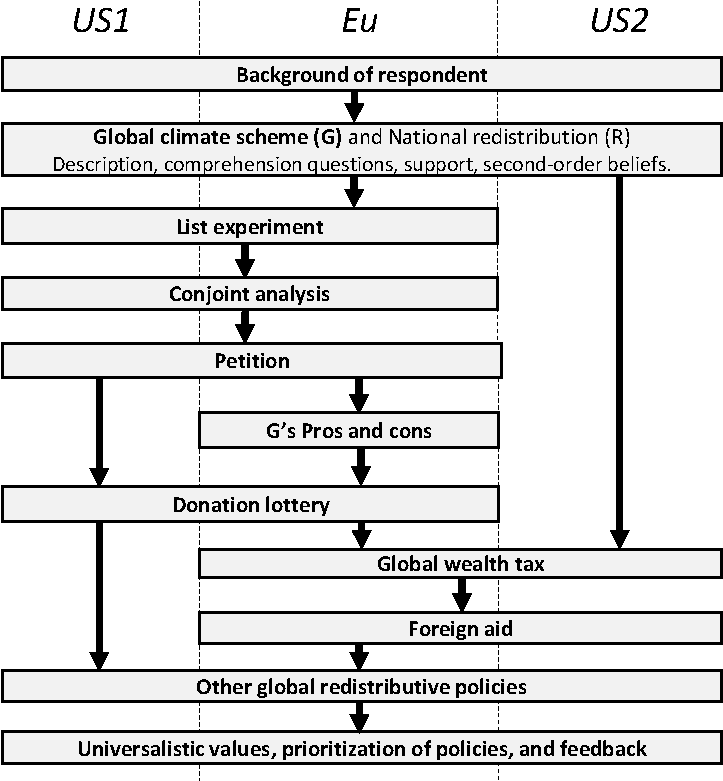
\includegraphics[width=.58\textwidth]{../questionnaire/survey_flow-simple.pdf}} 
% \end{figure}


The Western surveys ensured broad representativeness along key dimensions: gender, income, age, highest diploma, and degree of urbanization. The \textit{Eu} survey is also representative of its four countries in terms of population size, while the \textit{US1} and \textit{US2} surveys are representative in terms of region and ethnicity. 
Suppl. Tables S6-S7 %\ref{tab:representativeness_waves}-\ref{tab:representativeness_EU} 
detail how our samples match population frequencies. 
% Tables \ref{tab:representativeness_waves}-\ref{tab:representativeness_EU} confirm that our samples closely match population frequencies. 
More detail on data collection is given in Section \nameref{sec:methods}. The questionnaires used in the surveys are provided in S.I. C and D. % \ref{app:questionnaire_oecd} and \ref{app:questionnaire}.
% Details regarding the representativeness of the samples are provided in Tables \ref{tab:representativeness_waves}-\ref{tab:representativeness_EU}.



% \subsection{Stated support for global policies}\label{subsec:stated_support}

% The results from both the \textit{Global} and \textit{Complementary} surveys demonstrate robust support for global policies across all surveyed countries, with a clear preference for addressing climate action on a global scale over regional, national, or local approaches.

\subsection{Global support}\label{subsubsec:global_support}

We find strong support for climate policies enacted at the global level when analysing the global survey (Figure \ref{fig:oecd}). %, reproduced from \citealp{dechezlepretre_fighting_nodate}). 
When asked ``At which level(s) do you think public policies to tackle climate change need to be put in place?'', 70\% (in the U.S.) to 94\% (in Japan) choose the global level. The next most popular choice is the federal or continental level, favored by 52\% of Americans and less than half of European respondents. Local policies receive the least support. This preference for climate policies implemented at the global scale is in line with earlier contributions \cite{beiser-mcgrath_could_2019,bechtel_mass_2013,sivonen_attitudes_2022} %  
and consistent with individuals' concerns for the fairness and effectiveness of such policies, which have been identified as two of the three key determinants of support, besides self-interest.\citep{klenert_making_2018,douenne_yellow_2022,dechezlepretre_fighting_nodate} It could also stem from a preference for conditional cooperation,\citep{barrett_self-enforcing_1994} even if previous studies suggest that the support for climate policies does not depend on climate action abroad \citep{aklin_prisoners_2020,tingley_conditional_2014}. %


[Fig2] \refstepcounter{figure}\label{fig:oecd}
% \begin{figure}[h!]
  % MAJOR figure
%   \caption[Relative support for global climate policies]{Relative Support for global climate policies.} 
%   \makebox[\textwidth][c]{\includegraphics[width=1.2\textwidth]
%   {../figures/OECD/Heatplot_global_tax_attitudes_share.pdf}}\label{fig:oecd} % with dependence on others (absent from OECD): Heatplot_burden_share_all_share_countries
%   {\footnotesize \\ $\quad$ \\ Note 1: The numbers represent \textit{relative} support, i.e. the share of \textit{Somewhat} or \textit{Strongly support} among non-\textit{indifferent} answers (in percent, $n$ = 40,680). Shares of indifferent answers range from 11\% to 48\%, with quartiles 20\%, 27\%, and 33\%. The color blue denotes a relative majority. See Figure \ref{fig:oecd_absolute} for the absolute support. (Questions \ref{q:scale}-\ref{q:millionaire_tax}% Reproduced from \citealp{dechezlepretre_fighting_nodate}, Figure A21.
% ). \\ Note 2: *In Denmark, France and the U.S., the questions with an asterisk were asked differently, cf. Question \ref{q:burden_sharing_asterisk}. } 
% \end{figure}

Among the four global climate policies examined, three policies garner high support across all countries (Figure \ref{fig:oecd}). These policies include a global democratic assembly on climate change, a global tax on millionaires to finance low-income countries contingent on their climate action, and a global carbon budget of +2\textdegree{}C divided among countries based on tradable shares (or ``global quota''), with the allocation of country shares unspecified (see wording in S.I. C). %Appendix \ref{app:questionnaire_oecd}). 
%\footnote{The policies were all described with further details to make sure people understood them. Specifically, the policies were presented as follows: an international emissions trading system where ``countries that emit more than their national share would pay a fee to countries that emit less than their share''; ``a tax on all millionaires in dollars around the world to finance low-income countries that comply with international standards regarding climate action [which] would finance infrastructure and public services such as access to drinking water, healthcare, and education''; ``a global democratic assembly whose role would be to draft international treaties against climate change [where] each adult across the world would have one vote to elect members of the assembly''.} 
The three policies garner a majority of absolute support (i.e., ``somewhat'' or ``strong'' support) in all countries (except in the U.S. for the global assembly, 48\% absolute support). In high-income countries, the global quota policy obtains 64\% absolute support and 84\% relative support (i.e., excluding ``indifferent'' answers). %Support for this policy is even higher in middle-income countries, however their samples are only representative of the online population (young, graduated and urban people are over-represented).%due to the over-representation of young, educated, and urban populations in the online sample.
% done Several global policies obtain an absolute majority (i.e. \textit{somewhat} or \textit{strong}) %more than 70\% relative % support in all countries
% TODO? remove ", however their samples are only representative of the online population (young, graduated and urban people are over-represented)"

Following the support for the global quota, respondents are asked about their preferences for dividing the carbon budget among countries, as depicted in the third block of Figure \ref{fig:oecd}. Consistent with the existing literature (see S.I. A.1.2), %Appendix \ref{subsubsec:literature_attitudes_burden_sharing}),
an equal per capita allocation of emission rights emerges as the preferred burden-sharing principle, garnering absolute majority support in all countries and never below 84\% relative support. Taking into account historical responsibilities or vulnerability to climate damages is also popular, albeit with less consensus, while grandfathering (i.e., allocation of emission shares in proportion to current emissions) receives the least support in all countries.

A global carbon tax that funds a global basic income should produce the same distributional outcomes as a global tradable quota with equal per capita emission rights (to the extent that the carbon price is the same and provided that each country returns the revenues from emissions trading equally to its citizens). %\footnote{Similarly,  a global quota with grandfathering is equivalent to a global carbon tax where each country keeps the revenues it collects.} 
The support for the global carbon tax is also tested and its redistributive effects --  the average increase in expenditures along with the amount of the basic income -- are specified to the respondents explicitly  (see box below and S.I. D, p. 64). %Appendix \ref{app:questionnaire}, p.\pageref{subsec:questionnaire_GCS}). %: the \$30 per month basic income would lift the 700 million people who earn less than \$2/day out of extreme poverty, and fossil price increases would cost the typical person in their country a certain amount (that is provided).  % The average British person would lose a bit from this policy as they would face £42 per month in price increases, which is higher that the £22 they would receive.
The support for the carbon tax is lower than for the quota (t(34,442)=$-$76, P$<$0.001, difference=$-$.21), particularly in high-income countries (t(18,361)=$-$69, P$<$0.001, difference=$-$.28), and there is no relative majority for the tax in Anglo-Saxon countries (consistently with the levels of support found in the only previous study that tested a global carbon tax\cite{carattini_how_2019}). %\footnote{The levels of support are consistent with the findings of \citet{carattini_how_2019}, the only previous study that tested a global carbon tax.} 
Two possible reasons for this lower support are that distributive effects are specified explicitly in the case of the tax, and that people may prefer a quota, perhaps because they find it more effective than a tax to reduce emissions. The two reasons are consistent with the intermediate level of support for the GCS in the Western survey, which is based on a global quota but where the question specifies explicitly the distributive effects. %!
%The two reasons are consistent with the level of support for the global quota once we make the distributive effects salient in analysing support for the GCS in detail in the Western survey.

% One possible reason for this discrepancy is the explicit emphasis on the redistributive effects associated with the tax in the survey. The survey informs respondents that the \$30 per month basic income would lift 700 million people earning less than \$2/day out of extreme poverty, while fossil price increases would impose costs (specified in the survey) on the typical person in their country. Although other factors such as perceptions of effectiveness may also influence support for a quota versus a tax, this interpretation aligns with the level of support for the global quota when distributive effects are made salient, as we do in the complementary surveys. 

% The remainder of the paper analyzes the results from the complementary surveys in the U.S. and in Europe. This Section covers the stated support for different global redistributive policies. %the Global Climate Scheme, a global wealth tax, other global policies, and foreign aid.

%\subsubsection{Complementary surveys}

% \subsection{The Global Climate Scheme}\label{subsec:gcs}%\label{subsubsec:support_gcs}
%\paragraph{Global Climate Scheme}

\subsection{Stated support for the Global Climate Scheme}\label{subsec:gcs_stated_support}

The Western surveys (\textit{US1}, \textit{US2}, \textit{Eu}) include a comprehensive exploration of citizens' attitudes towards the GCS. We present to respondents a detailed description of the GCS and explain its distributive effects, including specific amounts at stake (as specified in the box below). Furthermore, we assess respondents' understanding of the GCS with incentivized questions to test their comprehension of the expected financial outcome for typical individuals in high-income countries (loss) and the poorest individuals globally (gain), followed by the provision of correct answers (Suppl. Figures S5-S6). % \ref{fig:understood_each}-\ref{fig:understood_score}). % TODO? That is, respondents are made aware and we find they understand that the policy will make people in their country poorer. 
% TODO? . 63\% understand the policy will make people in their country poorer, before even we indicate this as the right answer.

For comparison, %we also test support of conventional national redistribution: % 
the same approach is applied to a National Redistribution (NR) scheme targeting top incomes % the top 5\% (in the U.S.) or top 1\% (in Europe) 
with the aim of financing cash transfers to all adults, %\footnote{The wider base in the U.S. was chosen because emissions are larger in the U.S. than in Europe, and it would hardly be feasible to offset the median American's loss by taxing only the top 1\%.} 
calibrated to offset the monetary loss of the GCS for the median emitter in their country. We evaluate respondents' understanding that the richest would lose and the typical fellow citizens would gain from that policy. % done We proceed the same way for a National Redistribution Scheme (NR) that would tax the top 5\% (in the U.S.) or the top 1\% (in Europe) to finance cash transfers to all adults (calibrated to offset the monetary loss of the GCS for the median emitter), expecting people to find out at the comprehension question that the richest would lose and the typical people in their country would win.
Subsequently, we summarize both schemes to enhance respondents' recall. Additionally, we present a final incentivized comprehension question and provide the expected answer that the combined GCS and NR would result in no net gain or loss for a typical fellow citizen. Finally, respondents are directly asked to express their support for the GCS and NR using a simple \textit{Yes}/\textit{No} question.

\begin{tcolorbox}\label{box:GCS}
  \paragraph{The Global Climate Scheme} The GCS consists of global emissions trading with emission rights being auctioned each year to polluting firms, and of a global basic income, funded by the auction revenues. Using the price and emissions trajectories from the report by Stern \& Stiglitz,\cite{stern_report_2017} and in particular a carbon price of \$90/tCO$_\text{2}$ in 2030, we estimate that the basic income would amount to \$30 per month for every human adult %over the age of 15 
  (see details in S.I. E). %Appendix \ref{app:gain_gcs}). %, enough to lift out of extreme poverty the 700 million people who live with less than PPP \$2 per day. Conversely, assuming a carbon price of \$90/tCO$_\text{2}$ in 2030, high emitters like a typical American (with median U.S. CO$_\text{2}$ emissions) would lose in net \$85 per month, as they would face \$115 per month in price increases (see details in Appendix \ref{app:gain_gcs}). 
  We describe the GCS to the respondents as a ``climate club'' and we specify its redistributive effects: The 700 million people with less than \$2/day [in Purchasing Power Parity] would be lifted out of extreme poverty, and fossil fuel price increases would cost the typical person in their country a specified amount (see S.I. D %Appendix \ref{subsec:questionnaire_GCS} 
  for details). 
  The monthly median net cost is \$85 in the U.S., \euro{}10 in France, \euro{}25 in Germany, \euro{}5 in Spain, £20 in the UK.
\end{tcolorbox}

Our main result is that stated support for the GCS is 54\% in the U.S. and 76\% in Europe, while the support for NR is very similar: 56\% and 73\% respectively (Figures \ref{fig:support}, S3). %\ref{fig:support_binary}). 
% The 95\% confidence intervals are $[52.4\%, 55.9\%]$ in the U.S. and $[74.2\%, 77.2\%]$ in Europe. The average support is computed with survey weights, employing weights based on quota variables, which exclude vote. Another method to reweigh the raw results involves running a regression of the support for the GCS on sociodemographic characteristics (including vote) and multiplying each coefficient by the population frequencies. This alternative approach yields similar figures: 76\% in Europe and 52\% or 53\% in the U.S. (depending on whether individuals who did not disclose their vote are classified as non-voters or excluded). Notably, the average support excluding non-voters is 54\% in the U.S.
% Appendix \ref{app:determinants} 
S.I. F 
examines the sociodemographic determinants of support for the GCS as well as the beliefs correlated with the support for a global tax on GHG financing a global basic income. The strongest correlates are political leaning, trust in the government and perceptions that climate policies are effective at reducing emissions or in one's self-interest. 

Finding majority support for the GCS % runs counter to the conventional skepticism about the feasibility of global solidarity to addressing climate change. This % LM: I still agree with Thomas in the Overleaf comment.
motivates the subsequent analysis of robustness and sincerity. %, novel to attitudinal surveys on instrument choice for environmental policy.  %presents the sociodemographic determinants of GCS support, showing, for instance, stronger support among young people.
% Supplementary Section F examines the sociodemographic determinants of support for the GCS as well as the beliefs correlated with the support for a global tax on GHG financing a global basic income. The strongest correlates are political leaning, trust in the government and perceptions that the policy is effective at reducing emissions or in one's self-interest.

% \setcounter{figure}{0}
% \renewcommand{\thefigure}{S\arabic{figure}}
% \begin{figure}[h!]
%     \caption[Support for the Global Climate Scheme]{[For Supplementary Material, except first row to be included in Figure \ref{fig:support}] Support for the GCS, NR and the combination of GCS, NR and C (\textit{Yes}/\textit{No} questions). \\(p. \pageref{subsec:questionnaire_GCS}, Questions \ref{q:gcs_support}, \ref{q:nr_support}, \ref{q:global_tax}, \ref{q:national_tax}, and \ref{q:crg_support}).%; $n_\text{US} = n_\text{Eu} = 3,000,\, n_\text{FR} = 729,\, n_\text{DE} = 929,\, n_\text{ES} = 543,\, n_\text{UK} = 749$)
%     }\label{fig:support_binary}
%     \makebox[\textwidth][c]{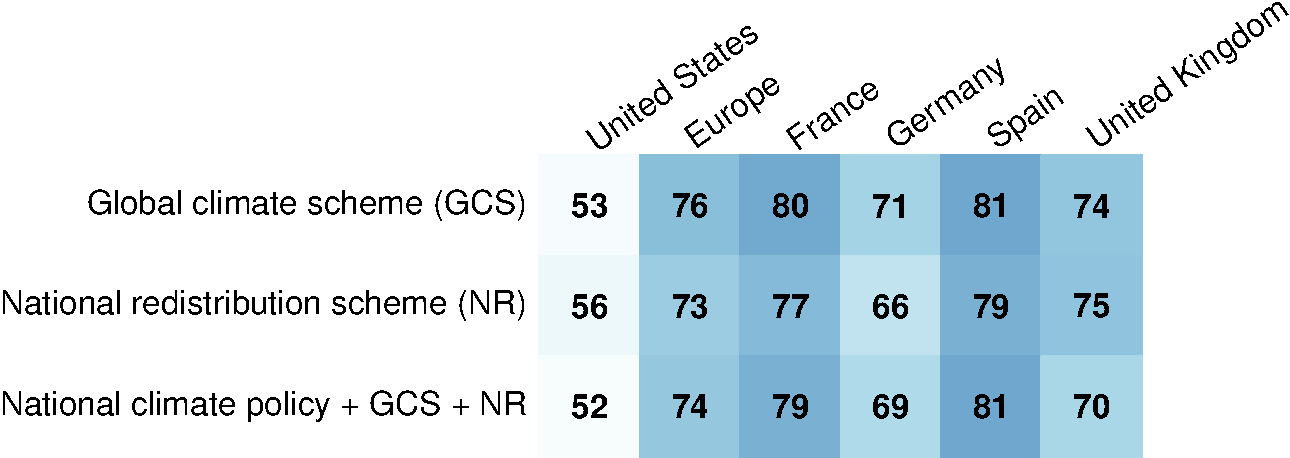
\includegraphics[width=.9\textwidth]{../figures/country_comparison/support_binary_positive.pdf}} 
% \end{figure}

\subsection{Robustness and sincerity of support for the GCS}\label{subsec:robustness_sincerity}


We use several methods to assess the sincerity of the support for the GCS: a list experiment, a real-stake petition, conjoint analyses, and an exercise involving the prioritization of policies. All methods suggest that the support is either completely sincere, or the share of insincere answers is limited. 

\subsubsection{List experiment}\label{subsubsec:list_exp} % NCCcomment

% A list experiment is employed to gauge tacit support for a specific policy of interest by asking respondents how many policies within a given list they support. By varying the list among respondents, the difference in number of policies supported can be used to estimate tacit support, revealing potential social desirability biases \citep{hainmueller_causal_2014}.
By asking \textit{how many} policies within a list respondents support and varying the list among respondents, a list experiment allows identifying the tacit support for a policy of interest. 
% The tacit support is estimated as the difference in the average number of policies supported between two groups, whose list differ only by the inclusion of that policy.\citep{hainmueller_causal_2014} % respondents who face a list containing the policy, and respondents who face the same list without it. 
For example, a first subsample faces the list of policies A, B, and C, while a second subsamples faces the list A, B, C, and GCS. We do not need to know which policies each respondent supports to estimate the average (tacit) support for the GCS, we simply need to compute the difference in the average number of supported policies between the two random subsamples.\citep{imai_multivariate_2011} 
% List experiments have been used to reveal social desirability bias, silencing either racism in the Southern U.S.\citep{kuklinski_racial_1997} or opposition to the invasion of Ukraine in Russia.\citep{chapkovski_solid_2022} % TODO? remove?
In our case, as shown in Table \ref{tab:list_exp}, the tacit support for the GCS measured through the list experiment is not significantly lower than the direct stated support. %\footnote{We utilize the difference-in-means estimator, and confidence intervals are computed using Monte Carlo simulation with the R package \textit{list}.\citep{imai_multivariate_2011}} 
Hence, we do not find a social desirability bias in our study.
% TODO? p-value?

% The tacit support for the GCS measured through the list experiment is as high as  the direct question in Eu but significantly lower by 5 p.p. in the U.S. This may be the sign of a social norm pushing some Americans to state that they support the GCS although they secretly do not. Still, if there is a social norm in favor of the GCS, there is a similar norm in favor of the National Redistribution Scheme, as the gap between the tacit and direct support for it is comparable (at 6 p.p.). %However, two observations qualify this interpretation. First, the gap between the tacit and direct support for the National Redistribution Scheme is comparable (at 7 p.p.) though we did not expect such a social norm in the case of the national redistribution, as the 95\% who would benefit from it should not feel ashamed to oppose a policy that would benefit them. Second, while we tested the questionnaire on random people in cafés, we noticed that some were confused by the question of the list experiment (asking how many policies from the list they supported), upset with the conservative societal policy (``Marriage only for opposite-sex couples in the U.S.'', ``Death penalty for major crimes'' in Europe), to the point that they did not answer attentively.

% \begin{table}[h]
%   % MAJOR figure % TODO! same table for NR in appendix
%   % TODO table by country
%   \caption[List experiment: tacit support for the GCS]{Number of supported policies in the list experiment depending on the presence of the Global Climate Scheme (GCS) in the list. %in function of the composition of the list. GCS stands for the Global Climate Scheme and NR for the National Redistribution Scheme.} % Beware, this question is quite unusual. \\ Among the policies below, how many do you support?  \\ Coal exit, Marriage only for opposite-sex couples 
%    The tacit support for the GCS is estimated by regressing the number of supported policies on the presence of the GCS in the list of policies. The social desirability is estimated as the difference between the tacit and stated support, and it is not significantly different from zero even at a 20\% threshold (see \nameref{sec:methods}).
%   }\label{tab:list_exp}
%   \makebox[\textwidth][c]{
\begin{tabular}{@{\extracolsep{5pt}}lccc} 
\\[-1.8ex]\hline 
\hline \\[-1.8ex] 
 & \multicolumn{3}{c}{Number of supported policies} \\ 
\cline{2-4} 
\\[-1.8ex] & All & US & Europe \\ 
\hline \\[-1.8ex] 
 List contains: GCS & 0.624$^{***}$ & 0.524$^{***}$ & 0.724$^{***}$ \\ 
  & (0.028) & (0.041) & (0.036) \\ 
\hline  \\[-1.8ex] \textit{Support for GCS} & 0.65  &  0.542  &  0.757 \\
\textit{Social desirability bias} & \textit{$ -0.026 $} & \textit{$ -0.018 $} & \textit{$ -0.033 $}\\
\textit{80\% C.I. for the bias} & \textit{ $[ -0.06 ; 0.01 ]$ } & \textit{ $[ -0.07 ; 0.01 ]$} & \textit{ $[ -0.08 ; 0.01 ]$}\\
 \hline \\[-1.8ex] 
Constant & 1.317 & 1.147 & 1.486 \\ 
Observations & 6,000 & 3,000 & 3,000 \\ 
R$^{2}$ & 0.089 & 0.065 & 0.125 \\ 
\hline 
\hline \\[-1.8ex] 
\textit{Note:}  & \multicolumn{3}{r}{$^{*}$p$<$0.1; $^{**}$p$<$0.05; $^{***}$p$<$0.01} \\ 
\end{tabular} 
%   }  
%   % {\footnotesize \textit{Note:} $^{*}p<0.1$; $^{**} p<0.05$; $^{***} p<0.01$.}
% \end{table}

% Donation addresses experimenter demand
\subsubsection{Petition}\label{subsubsec:petition} % Addresses hypothetical bias  % NCCcomment

% H1: Petition: Small effect against GCS: -4pp
We ask respondents whether they are willing to sign a petition in support of either the GCS or the NR policy. We inform them that the petition results will be sent to the head of state's office, highlighting the proportion of fellow citizens endorsing the respective scheme. Even when framed as a petition that might have real stakes, both policies continue to receive majority support. In the U.S., we find no significant difference between the support expressed in the %real-stake 
petitions question and the simple questions (GCS: t(3,044)=1.0, P=.297, difference=$-$.02, 95\% CI=[$-$.05, .02]; NR: t(2,952)=.3, P=.760, difference=$-$.01, 95\% CI=[$-$.04, .03]). 
%(GCS: $p=.30$; NR: $p=.76$). 
%\footnote{Paired weighted \textit{t}-tests are conducted to test the equality in support for a policy among respondents who were questioned about the policy in the petition.} 
In Europe, the petition leads to a comparable lower support for both the GCS, at $-$7 p.p. (t(3,018)=4.4, $P<0.001$, difference=$-$.07, 95\% CI=[$-$.10, $-$.04]) and NR, at $-$4 p.p. (t(2,953)=2.6, P=.008, difference=$-$.04, 95\% CI=[$-$.08, $-$.01]). 
%(7 p.p., $p=10^{-5}$) and NR (4 p.p., $p = .008$). 
While some European respondents are unwilling to sign a petition for policies they are expected to support, this phenomenon is not specific to the GCS, and the overall willingness to sign a %real-stake 
petition remains strong, with 69\% expressing support for the GCS and 67\% for NR.

\subsubsection{Conjoint analyses}\label{subsubsec:conjoint} % Addresses acquiescence bias  % NCCcomment
% H1, H2: Conjoint analysis: G|C+R 56%, G|R 59%, G 48% ~ C (|R), G+C|R 56%, C|R 64%, Left+G - Left = -3pp, A+G vs. B 59%
% => G is supported for itself, rather independently from R or C, with similar support to both, and it doesn't significantly penalize the Left, and would help a Democratic candidate

In order to assess the public support for the GCS in conjunction with other policies, we conduct a series of conjoint analyses. We ask respondents to make five choices between pairs of political platforms. Each choice is intended to test a different hypothesis about support for the GCS in relation to other policies or voting intentions.

The first conjoint analysis suggests that the GCS is supported independently of being complemented by the National Redistribution Scheme and a national climate policy (C). % (``Coal exit'' in the U.S., ``Thermal insulation plan'' in Europe, denoted C).
%\footnote{Indeed, 54\% of %($n$ = 3,000) 
% U.S. respondents and 74\% of %($n$ = 3,000) 
% European ones prefer the combination of C, NR and the GCS to the combination of C and NR alone, indicating similar support for the GCS conditional on NR and C than for the GCS alone (Figure \ref{fig:conjoint}).} % (as it does not significantly differ from the direct support of 53\%). 
% For the second analysis, we split the sample into four random branches (see \nameref{sec:methods}). 
% % \footnote{Results from the first branch show that the support for the GCS conditional on NR, at 55\% in the U.S. ($n$ = 757) and 77\% in Europe ($n$ = 746), is not significantly different from the support for the GCS alone. This suggests that rejection of the GCS is not driven by the cost of the policy on oneself. The second branch shows that the support for C conditional on NR is somewhat higher, at 62\% in the U.S. ($n$ = 751) and 84\% in Europe ($n$ = 747). However, the third one shows no significant preference for C compared to GCS (both conditional on NR), neither in Europe, where GCS is preferred by 52\% ($n$ = 741) nor in the U.S., where C is preferred by 53\% ($n$ = 721). The fourth branch shows that 55\% in the U.S. ($n$ = 771) and 77\% in Europe ($n$ = 766) prefer the combination of C, NR and the GCS to NR alone.} 
% The outcome is that there is
The second analysis indicates majority support for the GCS and for C, which are seen as neither complement nor substitute (see \nameref{sec:methods}). A minor share of respondents like a national climate policy and dislike a global one, but as many people prefer a global rather than a national policy. Besides, there is no evidence that implementing NR would increase the support for the GCS.


In the third analysis, we present two random branches of the sample with hypothetical progressive and conservative platforms that differ only by the presence (or not) of the GCS in the progressive platform. Table \ref{tab:conjoint_c} shows that a progressive candidate would not significantly lose voting share by endorsing the GCS in any country, and may even gain 11 p.p. in voting intention in France. % (t(605)=2.7, $P = .007$, 95\% CI=[.03, .19]). %The effect is also positive at 3 p.p. ($p = .13$) in the U.S., although not significant at the 5\% threshold. % France holds multiple hypotheses testing

% Though the level of support for the GCS is significantly lower in swing States (at 51\%) that are key to win U.S. elections, the electoral effect of endorsing the GCS remains non-significantly different from zero (at +1.2 p.p.) in these States.
% \footnote{We define swing states as the 8 states with less than 5 p.p. margin of victory in the 2020 election (MI, NV, PA, WI, AZ, GA, NC, FL). The results are robust to using the 3 p.p. threshold (that excludes FL) instead.}

%The third analysis suggests that a progressive candidate would not significantly lose voting share if he or she were to endorse the GCS, and that he or she may even gain 11 p.p. vote intention in France (see Table \ref{tab:conjoint_c}). To estimate this, we present to two random branches of the sample hypothetical progressive and conservative platforms that differ only by the presence (or not) of the GCS in the progressive platform. 

% \begin{table}[h]
%   % MAJOR figure
%   \caption[Influence of the GCS on electoral prospects]{Preference for a progressive platform depending on whether it includes the GCS or not. (Question \ref{q:conjoint_c}) 
%   %Imagine if the [Democratic and Republican presidential candidates in 2024] campaigned with the following policies in their platforms. [Credible Progressive and Conservative platforms] \\ % TODO See More
% % Which of these candidates would you vote for? \textit{A; B; None of them} \\
% % ~[FR: second round of presidential; DE, ES, UK: two favorite candidates in one's constituency]
% } % Beware, this question is quite unusual. \\ Among the policies below, how many do you support?  \\ Coal exit, Marriage only for opposite-sex couples 
%   \makebox[\textwidth][c]{
\begin{tabular}{@{\extracolsep{5pt}}lcccccc} 
\\[-1.8ex]\hline 
\hline \\[-1.8ex] 
 & \multicolumn{6}{c}{Prefers the Progressive platform} \\ 
\cline{2-7} 
\\[-1.8ex] & All & United States & France & Germany & UK & Spain \\ 
\hline \\[-1.8ex] 
 GCS in Progressive platform & 0.028$^{*}$ & 0.029 & 0.112$^{***}$ & 0.015 & 0.008 & $-$0.015 \\ 
  & (0.014) & (0.022) & (0.041) & (0.033) & (0.040) & (0.038) \\ 
 \hline \\[-1.8ex] 
Constant & 0.623 & 0.604 & 0.55 & 0.7 & 0.551 & 0.775 \\ 
Observations & 5,202 & 2,619 & 605 & 813 & 661 & 504 \\ 
R$^{2}$ & 0.001 & 0.001 & 0.013 & 0.0003 & 0.0001 & 0.0003 \\ 
\hline 
\hline \\[-1.8ex] 
\end{tabular} 
}\label{tab:conjoint_c}
%   {\footnotesize \textit{Note:} Simple OLS model. The 14\% of \textit{None of them} answers have been excluded from the regression samples. GCS has no significant influence on them. $^{*}p<0.1$; $^{**} p<0.05$; $^{***} p<0.01$. 
%   }
% \end{table}
% \begin{stretchpars}

Our last two analyses make respondents choose between two random platforms. In Europe, respondents are prompted to imagine that a left or center-left coalition will win the next election and asked what platform they would prefer that coalition to have campaigned on. In the U.S., the question is framed as a hypothetical duel in a Democratic primary, and asked only to non-Republicans ($n$ = 2,218), i.e. the respondents who declare as political affiliation \textit{Democrat}, \textit{Independent}, \textit{Non-Affiliated} or \textit{Other}. 

In the fourth analysis, a policy (or an absence of policy) is randomly drawn for each platform in each of five categories: \textit{economic issues}, \textit{societal issues}, \textit{climate policy}, \textit{tax system}, \textit{foreign policy} (Figure \ref{fig:ca_r}, Table \ref{tab:amce}). 
% Except for the category \textit{foreign policy}, which features the GCS 42\% of the time, the policies are prominent progressive policies and they are drawn uniformly. % except for tax1: .35 vs. tax2: .4 in EU. 
In the UK, Germany, and France, a platform is about 9 to 13 p.p. more likely to be preferred if it includes the GCS rather than no foreign policy. %\footnote{This is the Average Marginal Component Effect.\cite{hainmueller_causal_2014}} 
This effect is between 1 and 4 p.p. and no longer significant in the U.S. (among non-Republicans) and in Spain. Moreover, a platform that includes a global tax on millionaires rather than no foreign policy is 5 to 13 p.p. more likely to be preferred in all countries (the effect is significant and at least 9 p.p. in all countries but Spain). 
% Moreover, a platform that includes a global tax on millionaires rather that no foreign policy is 9 to 13 percentage points (p.p.) more likely to be preferred in all countries but Spain (not significant, at +5 p.p.). 
Similarly, a global democratic assembly on climate change has a significant effect of 8 to 12 p.p. in the U.S. (among non-Republicans), France, and Germany (this echoes earlier findings on global democracy\citep{ghassim_who_2020}). 
%In each country, a platform is more likely to be preferred if it includes the GCS rather than no foreign policy. This effect is significant in France, Germany and the UK, where a platform is about 10 p.p. more likely to be preferred. 
These effects are large, and not far from the effects of the policies most influential on the platforms, which range between 15 and 18 p.p. in most countries (27 p.p. in Spain), and all relate to improved public services (in particular healthcare, housing, and education).
% \end{stretchpars}
 
% \begin{figure}[h] 
%   \caption[Preferences for various policies in political platforms]{[For Supplementary Material] Effects of the presence of a policy (rather than none from this domain) in a random platform on the likelihood that it is preferred to another random platform. (See non-translated versions in Figure \ref{fig:ca_r_en}; Question \ref{q:conjoint_r}%; in the U.S., asked only to non-Republicans.
%   )}\label{fig:ca_r}
%   \begin{subfigure}{\textwidth}
%     \subcaption{U.S. (Asked only to non-Republicans)}
%     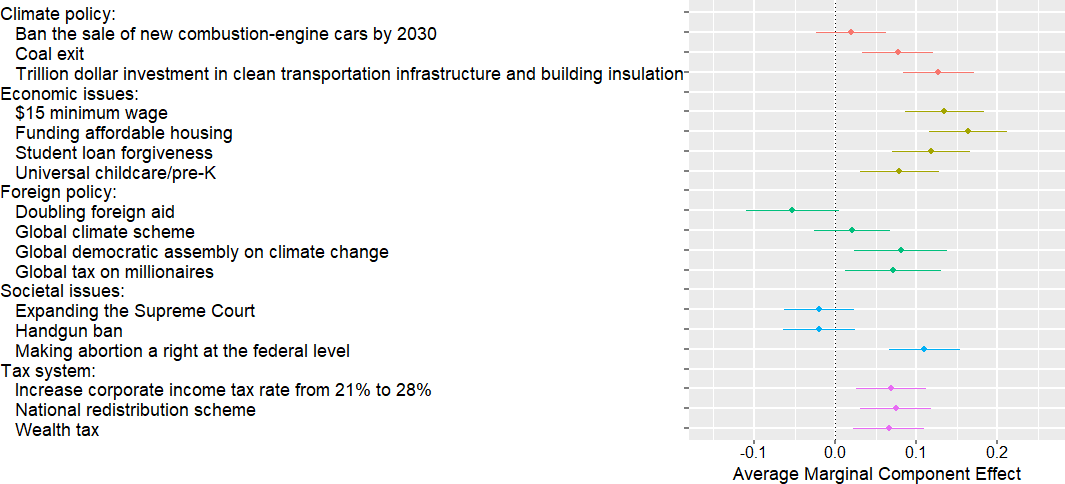
\includegraphics[width=\textwidth]{../figures/US1/ca_r.png}
%   \end{subfigure}
%   \begin{subfigure}{\textwidth}
%     \subcaption{France}
%     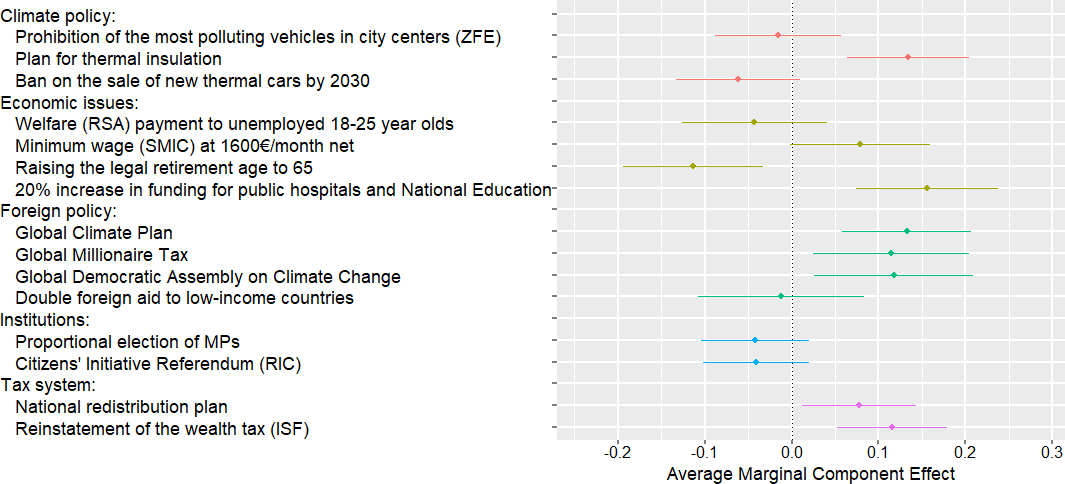
\includegraphics[width=\textwidth]{../figures/FR/ca_r_en.png}
%   \end{subfigure}
% \end{figure}%
% \clearpage
% \begin{figure}[h!]\ContinuedFloat % if bugs try b! instead of h!
%   \begin{subfigure}{\textwidth}
%     \subcaption{Germany}
%     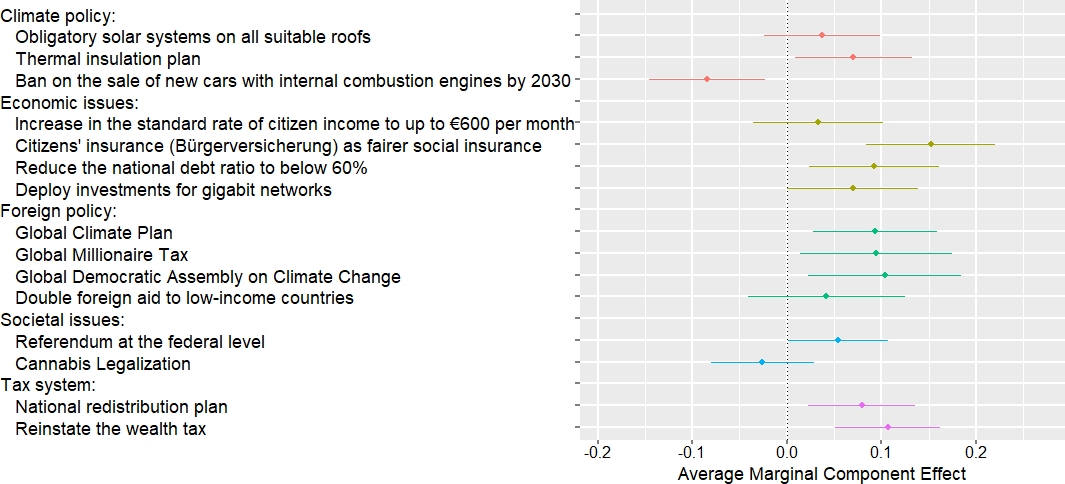
\includegraphics[width=\textwidth]{../figures/DE/ca_r_en.png}
%   \end{subfigure}
%   \begin{subfigure}{\textwidth}
%     \subcaption{Spain}
%     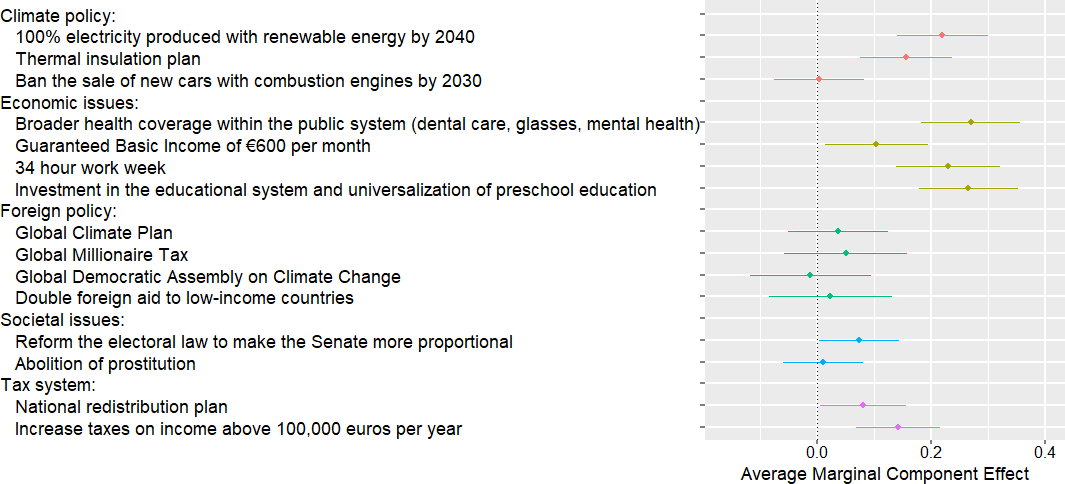
\includegraphics[width=\textwidth]{../figures/ES/ca_r_en.png}
%   \end{subfigure}
%   \begin{subfigure}{\textwidth}
%     \subcaption{UK}
%     \includegraphics[width=\textwidth]{../figures/UK/ca_r.png}
%   \end{subfigure}
%   %\makebox[\textwidth][c]{} 
% \end{figure}
% \clearpage 
% \noindent 
The fifth analysis draws random platforms similarly, except that candidate A's platform always contains the GCS while B's includes no foreign policy. In this case, A is chosen by 60\% of Europeans %($n$ = 3,000) 
and 58\% of non-Republican Americans (Figure \ref{fig:conjoint_left_ag_b}). %($n$ = 2,218). 

Overall, taking the U.S. as an example, our conjoint analyses indicate that a candidate at the Democratic primary would have more chances to obtain the nomination by endorsing the GCS, and this endorsement would not penalize her or him at the presidential election. 
%This result relates to the finding that 12\% of Germans shift their voting intention from SPD and CDU/CSU to the Greens and the Left when they are told that the latter parties support global democracy.\citep{ghassim_who_2020}


% \begin{figure}[h!]
%     \caption[Influence of the GCS on preferred platform]{[For Supplementary Material] Influence of the GCS on preferred platform:\\ Preference for a random platform A that contains the Global Climate Scheme rather than a platform B that does not (in percent). (Question \ref{q:conjoint_d}; in the U.S., asked only to non-Republicans.)}\label{fig:conjoint_left_ag_b}
%     \makebox[\textwidth][c]{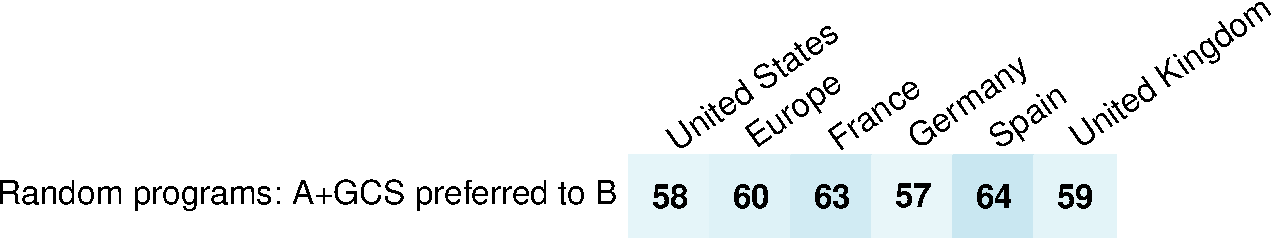
\includegraphics[width=\textwidth]{../figures/country_comparison/conjoint_left_ag_b_binary_positive.pdf}} 
% \end{figure}


% \begin{figure}
%   % Imagine that at the 2024 Democratic party presidential primaries, the two main candidates campaign with the following key policies in their platforms. \\ Which of these candidates do you prefer?

%   \caption{Conjoint analysis. Average Marginal Component Effects (relative to the baseline: an absence of policy of that category) of policies in the choice between two platforms, where policies in each platform are randomly drawn ($n$ = 6,000). In Eu, it is framed as two potential platforms of a left-wing coalition that would win the next elections; in the U.S., it is framed as a hypothetical duel in the 2024 Democratic primary and asked only to non-Republicans.}\label{fig:ca_r} % TODO: add ref to Question
%   \makebox[\textwidth][c]{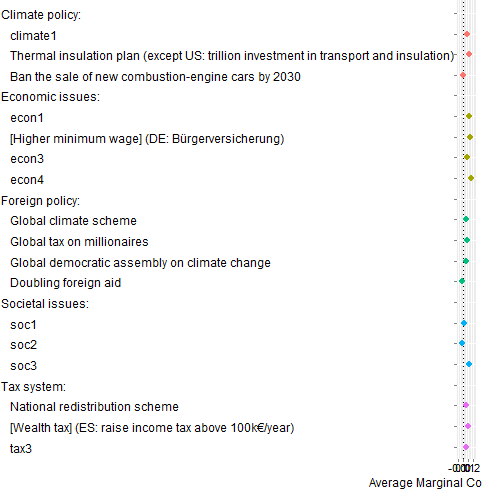
\includegraphics[width=\textwidth]{../figures/all/ca_r.png}}
% \end{figure}

\subsubsection{Prioritization}\label{subsubsec:prioritization} % Addresses acquiescence bias and social desirability bias
% H1: Prioritization: G has mean only slightly lower than average, makes better than ban of cars and coal exit; global tax on millionaires does as well as wealth tax and almost as good as $15 minimum wage

Towards the end of the survey, we ask respondents to allocate 100 points among six randomly selected policies from the previous conjoint analyses, using sliders. The instruction was to distribute the points based on their level of support, with a higher allocation indicating greater support for a policy. %At the end of the survey, we pick six policies at random (and uniformly) among the policies used in the last conjoint analyses, and ask respondents to allocate 100 points among them (using sliders), with the instruction that ``the more you give points to a policy, the more you support it''. 
As a result, the average support across policies is 16.67 points. %(Figure \ref{fig:points}). % TODO! figures for each country
In each country, the GCS ranks in the middle of all policies or above, with an average number of points from 15.4 in the U.S. to 22.9 in Germany.%The GCS ranked in the middle or higher among all policies in each country, receiving an average of 15.4 points in the U.S. and 22.9 points in Germany.

Interestingly, in Germany, the most prioritized policy is the global tax on millionaires, while the GCS is the second most prioritized policy. The global tax on millionaires consistently ranks no lower than fifth position (out of 15 or 17 policies) in every country, garnering an average of 18.9 points in Spain to 22.9 points in Germany.

% This question sheds light on a potential discrepancy between the policy priorities of the public and those enacted by legislators. For instance, while the European Union and California have enacted plans to phase out new combustion-engine cars by 2035, the proposal to ``ban the sale of new combustion-engine cars by 2030'' emerged as one of the three least prioritized policies in each country, with an average allocation of 7.8 points in France to 11.4 points in the UK.

%It is higher than to ``ban the sale of new combustion-engine cars by 2030'' (13.4) and ``coal exit'' (10.0), but lower than the third climate policy: ``trillion dollar investment in clean transportation infrastructure and building insulation'' (20.3). The support for other globally redistributive policies is variable: ``Doubling foreign aid'' is the least supported policy (8.4), while the ``Global tax on millionaires'' is one of the five policies with more than 20 points (20.2), and the ``global democratic assembly on climate change'' is just below the GCS (14.5). The most supported policies are ``Funding affordable housing'' (28.5), ``\$15 minimum wage'' (23.8), and ``Universal childcare/pre-K'' (22.1). % TODO? share that allocated at least 1

% \begin{figure}[h!]
%   \caption{Prioritization of policies. Each respondent faces six policies taken at random from the ones below and allocates 100 points among them to signal the strength of their support for each one ($n$ = 3,000).} % Imagine you have 100 points that you can allocate to different policies. The more you give points to a policy, the more you support it.  \\  How do you allocate the points among the following policies?  
  
%   \makebox[\textwidth][c]{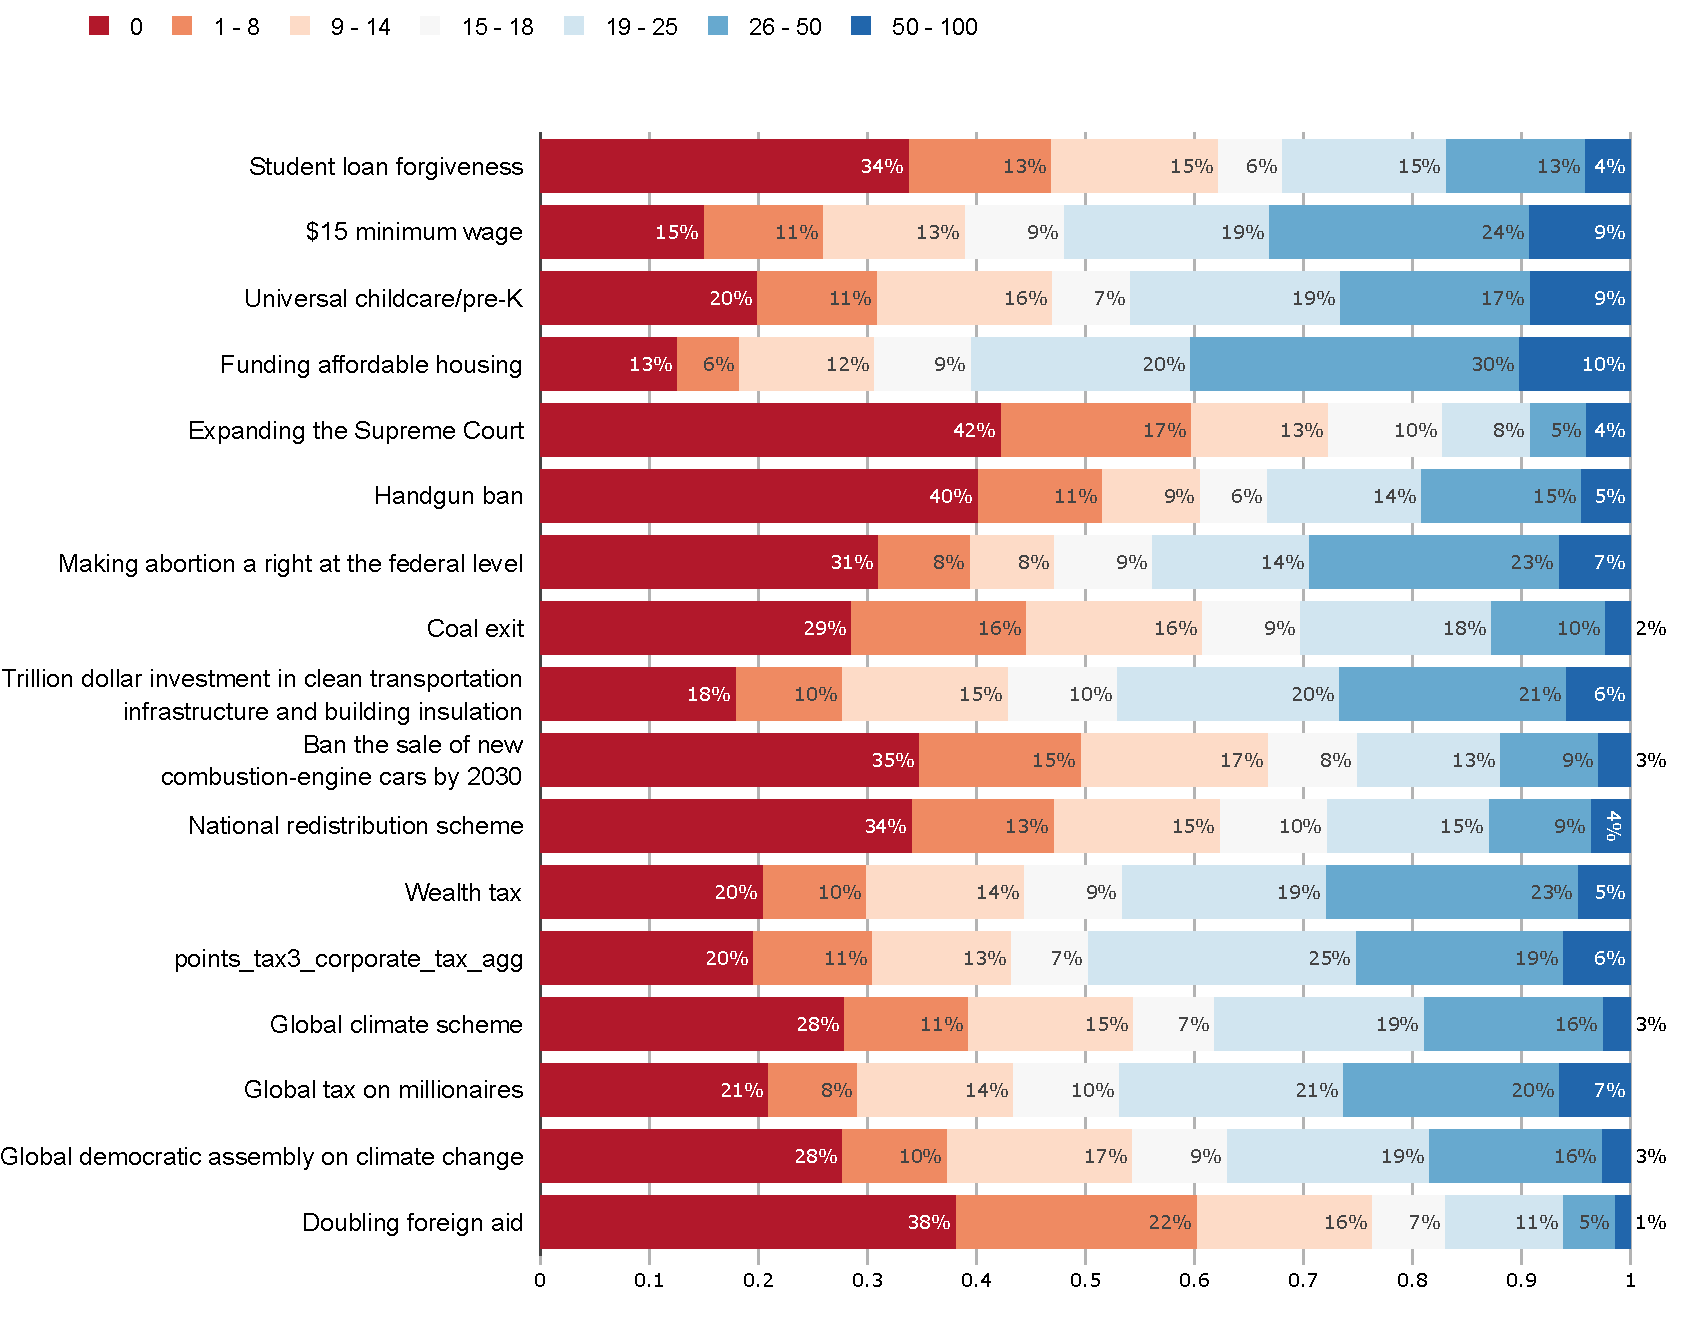
\includegraphics[width=\textwidth]{../figures/US1/points_us.pdf}}\label{fig:points}
% \end{figure}

% TODO? This slightly differs from a conjoint analysis, which only allows inferring individual-level preferences for one platform over another or collective-level preferences for one policy over another. Also, by comparing platforms, conjoint analyses may be subject to interaction effects between policies of a platform (which can be seen as Main, subsitute, or antagonistic) while the prioritization frames the policies as independent.

\subsubsection{Pros and Cons}\label{subsubsec:pros_cons}

We survey respondents to gather their perspectives on the pros and cons of the GCS, randomly utilizing an open-ended or a closed question. In the closed question format, respondents tend to consider every argument as important in determining their support or opposition to the GCS (see Suppl. Figure S10). %\ref{fig:gcs_important}). 
% Notably, the least important aspect was the negative impact on their household, with 60\% in Europe ($n$=1,505) and 75\% in the U.S. ($n$=493) finding it important. The most important elements differ between Europe and the U.S. In Europe, the key factors are the GCS's potential to limit climate change and reduce poverty in low-income countries, both deemed important by 85\% of respondents. In the U.S., having sufficient information about the scheme ranks highest at 89\%, followed by its potential to foster global cooperation at 82\%. However, d
% Due to the limited variation in the ratings for each element, the closed question format is inconclusive (Figure \ref{fig:gcs_important}). % TODO? distinguish between supporters and opponents?
% TODO? cite figure 

The open-ended question provides more insights into what people associate with the GCS when prompted to think about it. % The open-ended question gives interesting insight into ``what comes to [people's] mind'' when ``thinking of the GCS''. 
Analyzing keywords in the responses (automatically translated into English), the most frequently mentioned topics are the international dimension and the environment, each appearing in approximately one-quarter of the answers (see Suppl. Figure S12). %\ref{fig:gcs_field_contains}). 
This is followed by discussions on the effects of the GCS on poverty and prices, each mentioned by about one-tenth of the respondents. We also manually classified each answer into different categories (see Suppl. Figure S11). % \ref{fig:gcs_field}). 
This exercise confirms the findings from the automatic search: the environmental benefit of the GCS is the most commonly discussed topic, while obstacles to implementation or agreement on the proposal are relatively infrequently mentioned.%the most frequent topic is the environmental benefit of the GCS, while the obstacles to implement it or to get %people or countries agreement on it are relatively seldom mentioned.
% \footnote{Moreover, around one in four respondents explicitly cites pros or cons. Few individuals explicitly express support or opposition, and misunderstandings are rare. Only 11\% of the responses are empty or express a lack of opinion, though one-quarter are unclassifiable due to the rarity, nonsensical nature, or irrelevance of the conveyed idea.}% TODO n

% In the \textit{US2} survey, we presented these questions to random subsamples \textit{before} inquiring about support for the GCS or NR. The sample was divided into four branches: two branches with questions on pros and cons (either in closed or open form), one branch providing information on the actual level of support for the GCS and NR (estimated in \textit{US1}), and one control group without these questions.\footnote{Consistent with Americans accurately perceiving the levels of support for the GCS or NR, providing information on the actual level had no substantial effect on their support. In the closed question regarding pros and cons, we intentionally included more cons (6) than pros (3) to conservatively estimate the potential campaign effect on the GCS, which refers to the shift in opinion resulting from media coverage of the proposal. Interestingly, the support for the GCS decreased by 11 p.p. after respondents viewed a list of its pros and cons. Surprisingly, the support for National Redistribution also decreased by 7 p.p. following the closed question about the GCS. This suggests that some individuals may lack attention and confuse the two policies, or that contemplating the pros and cons alters the mood of some people, moving them away from their initial positive impression. Notably, the support also decreased by 7 p.p. after respondents were asked to consider the pros and cons in an open-ended question.} Despite some significant effects of pondering the pros and cons (see Table \ref{tab:branch_gcs}), approximately half of the Americans expressed support for the GCS across all treatment branches. If similar effects were observed in Europe, it suggests that the GCS would still enjoy strong majority support among Europeans once it enters the public debate (Table \ref{tab:branch_gcs}).


In the \textit{US2} survey, we divided the sample into four random branches. Two branches were presented the pros and cons questions (either in open or closed format) \textit{before} being asked about their support for the GCS or NR. Another branch received information on the actual level of support for the GCS and NR (estimated in \textit{US1}, see box p. \pageref{subsec:second_order_beliefs}), %Section \ref{subsec:second_order_beliefs}), 
and one control group received none of these treatments. % TODO? Clarify that the information was also before the support? Write here (rather than in second-order beliefs) that ``Consistent with Americans correctly perceiving the levels of support for the GCS or NR, providing information on the actual level has no substantial effect on their support.''
The objective of the ``pros and cons treatment'' was to mimic a ``campaign effect'', which refers to the shift in opinion resulting from media coverage of the proposal.\citep{gustafson_development_2019,anderson_can_2023} To conservatively estimate the effect of a (potentially negative) campaign, we intentionally included more cons (6) than pros (3). Interestingly, the support for the GCS decreased by 11 p.p. (t(1,996)=$-$3.5, $P<0.001$, difference=$-$.11, 95\% CI=[$-$.17, $-$.05]) after respondents viewed a list of its pros and cons. %\footnote{Surprisingly, the support for National Redistribution also decreased by 7 p.p. following the closed question about the GCS. This suggests that some individuals may lack attention and confuse the two policies, or that contemplating the pros and cons alters the mood of some people, moving them away from their initial positive impression.} 
Notably, the support also decreased by 7 p.p. (t(1,996)=$-$2.3, P=.020, difference=$-$.07, 95\% CI=[$-$.13, $-$.01]) after respondents were asked to consider the pros and cons in an open-ended question. Despite some significant effects of pondering the pros and cons, approximately half of the Americans express support for the GCS across all treatment branches (see Table \ref{tab:branch_gcs}). Although support remains significant, % relatively high (it would remain majoritarian in Europe if similar effects were observed)
these results suggest that the public success of the GCS would be sensitive to the content of the debate about it, and oriented by the discourse adopted by interest groups. %  TODO? support for the GCS is context-dependent

% where respondents are prompted to think about the advantages and drawbacks of the policy before making a decision

% On the campaign effect: Funk (16) shows that there is a survey bias of 5-6 p.p.: in post-referendum surveys, Swiss people approve left-wing policies 5 pp less. Jenning & Wlezien (18) show that between seven to one month before the election, polls mean absolute error about the result is ~4 p.p. (goes down to ~2pp the days before).




\begin{tcolorbox}\label{subsec:second_order_beliefs}
  \paragraph{Second-order Beliefs}
% \subsection{Second-order Beliefs}\label{subsec:second_order_beliefs}
% H3 belief: No pluralistic ignorance
To explain the strong support for the GCS despite its absence from political platforms and public debate, we hypothesized pluralistic ignorance, i.e. that the public and policymakers mistakenly perceive the GCS as unpopular. As a result, individuals might conceal their support for such globally redistributive policy, believing that advocating for it would be futile. 
% However, the evidence for pluralistic ignorance is limited based on an incentivized question about perceived support (Figure \ref{fig:belief}).

In the case of Americans, their beliefs about the level of support for the GCS are relatively accurate (Figure \ref{fig:belief}). The mean perceived support is 52\% (with quartiles of 36\%, 52\%, and 68\%), which closely aligns with the actual support of 54\%. Europeans, on the other hand, underestimate the support by 17 p.p. Nonetheless, 65\% of them correctly estimate that the GCS garners majority support, and the mean perceived support is 59\% (and quartiles of 43\%, 61\%, and 74\%), compared to the actual support of 76\%. % TODO? cut below?
Second-order beliefs are equally accurate for NR in the U.S. and similarly underestimated in Europe. %, with mean (resp. quartiles) perceived support of 54.7\% (resp. 40, 55, 71\%, $n$ = 3,000) vs. 56\%.
Finally, consistent with Americans accurately perceiving the levels of support for the GCS or NR, providing information on the actual level had no significant effect on their support in the \textit{US2} survey (effect=.025, t(1,998)=1.1, P=.262, 95\% CI=[$-$.02, .07]). % Consistent with Americans correctly perceiving the levels of support for the GCS or NR, providing information on the actual level has no substantial effect on their support.
\end{tcolorbox}

% \begin{figure}[h!]
%     \caption[Beliefs about support for the GCS and NR]{[For Supplementary Material] Beliefs regarding the support for the GCS and NR. (Questions \ref{q:gcs_belief} and \ref{q:nr_belief})}\label{fig:belief}
%     \makebox[\textwidth][c]{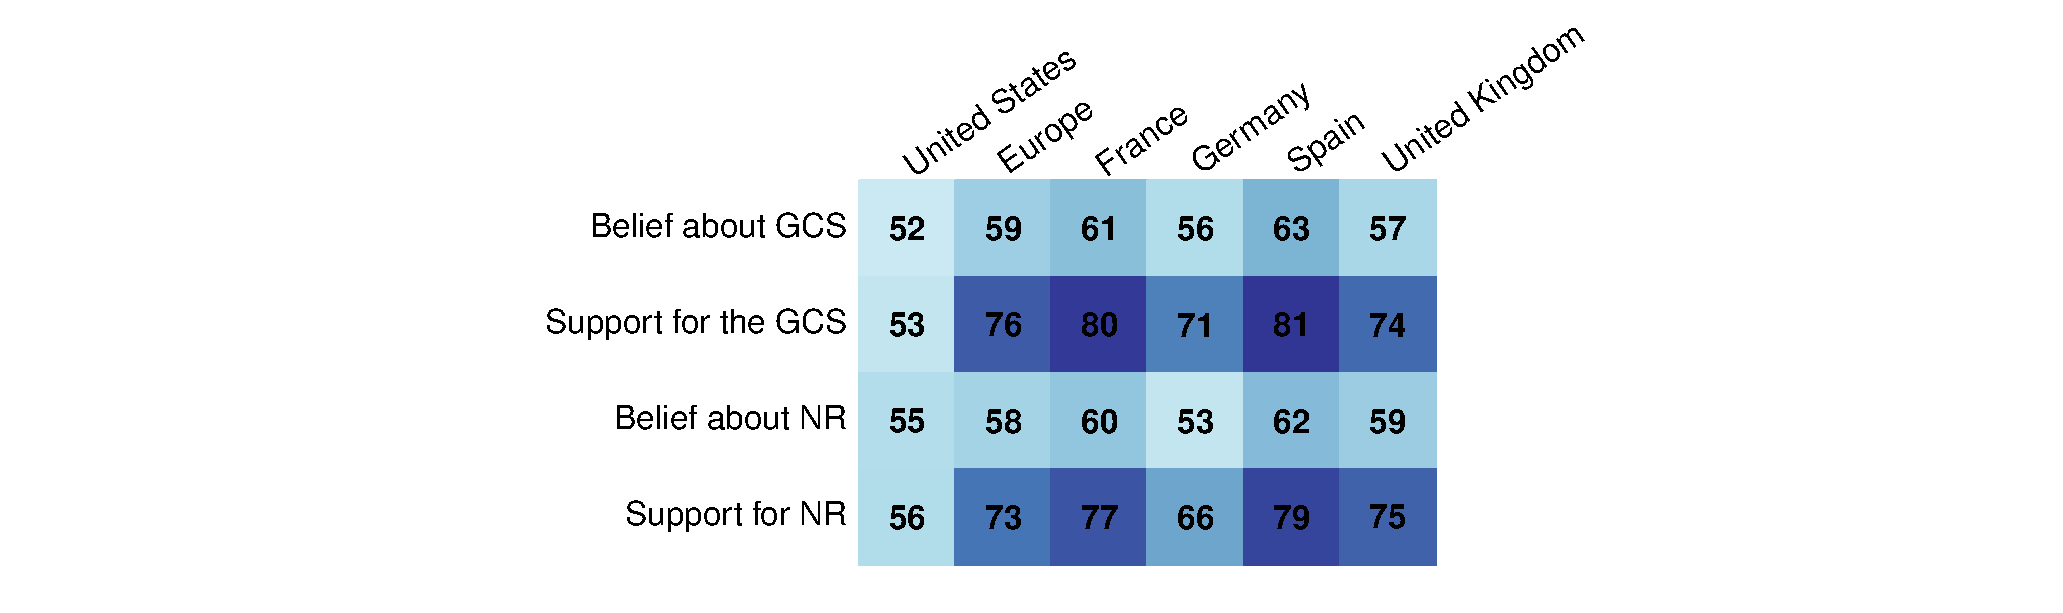
\includegraphics[width=.7\textwidth]{../figures/country_comparison/belief_all_mean.pdf}} 
% \end{figure}

\subsection{Stated support for global redistribution}\label{subsec:support_other}


We also assess support for a range of other international policies (Figure \ref{fig:support}) as well as unilateral foreign aid. %to be able to compare the support for the objectives of environmental protection and redistribution, including foreign aid, separately. 


\subsubsection{International policies}\label{subsubsec:support_other_global_policies} % NCCcomment
% \paragraph{Other global policies}

Most policies garner relative majority support in each country, with two exceptions: the ``cancellation of low-income countries' public debt'' and ``a maximum wealth limit'' for each individual (Figure \ref{fig:support}). % In US pilot (n=86), 36% relative support to cap wealth at 100M (67% in Eu)
There is relative majority support for it in Europe but not in the U.S., despite the cap being set at \$10 billion in the U.S. compared to \euro{}/£100 million in Europe. Notably, climate-related policies enjoy significant popularity, with ``high-income countries funding renewable energy in low-income countries'' receiving absolute majority support in all countries surveyed. Additionally, relative support for loss and damages compensation, as approved in principle at the international climate negotiations in 2022 (``COP27''), ranges from 55\% (U.S.) to 81\% (Spain). %, with absolute support ranging from 41\% to 62\%.

%\subsubsection{Global wealth tax}\label{subsubsec:support_global_wealth_tax}
%\paragraph{Global wealth tax}

Consistent with the results of the global survey, 
a ``tax on millionaires of all countries to finance low-income countries'' garners relative support of 69\% in the U.S. and 84\% in Europe, only 3 p.p. lower than a national millionaires tax overall (t(4,243)=$-$2.2, P=.028, difference=$-$.03, 95\% CI=[$-$.05, $-$.00]). In random subsamples, we also inquire about respondents' preferences regarding the redistribution of revenues from a global tax on individual wealth exceeding \$5 million, after providing information on the revenue raised by such a tax in their country compared to low-income countries. 
% \footnote{A 2\% tax on net wealth exceeding \$5 million would annually raise \$816 billion, leaving unaffected 99.9\% of the world population. More specifically, it would collect \euro{}5 billion in Spain, \euro{}16 billion in France, £20 billion in the UK, \euro{}44 billion in Germany, \$430 billion in the U.S., and \$1 billion collectively in all low-income countries (28 countries, home to 700 million people).%Figures come from \citet{chancel_world_2022}, the \href{https://wid.world/world-wealth-tax-simulator/}{WID wealth tax simulator}, and the World Bank. % TODO: do they?
% } 
We ask certain respondents ($n$ = 1,283) what percentage of the global tax revenues should be pooled to finance low-income countries. In each country, at least 88\% of respondents indicate a positive amount, with an average of one-third %ranging from 30\% (Germany) to 36\% (U.S., France) 
(Figure \ref{fig:global_share_mean}). To other respondents ($n$ = 1,233), we inquire whether they would prefer each country to retain all the revenues it collects or that half of the revenues be pooled to finance low-income countries. Approximately half of the respondents opt to allocate half of the tax revenues to low-income countries, consistently with the other variant of the question.

% \begin{figure}
%     \centering 
%     \caption[Preferred share of wealth tax for low-income countries]{[For Supplementary Material] Percent of global wealth tax that should finance low-income countries (\textit{mean}). \\ ``Imagine a wealth tax on households with net worth above [\$]5 million, enacted in all countries around the world.  
%     (\dots)  \\
%     What percentage should be pooled to finance low-income countries (instead of retained in the country's national budget)?'' (Question \ref{q:global_tax_global_share})} % TODO? n
%     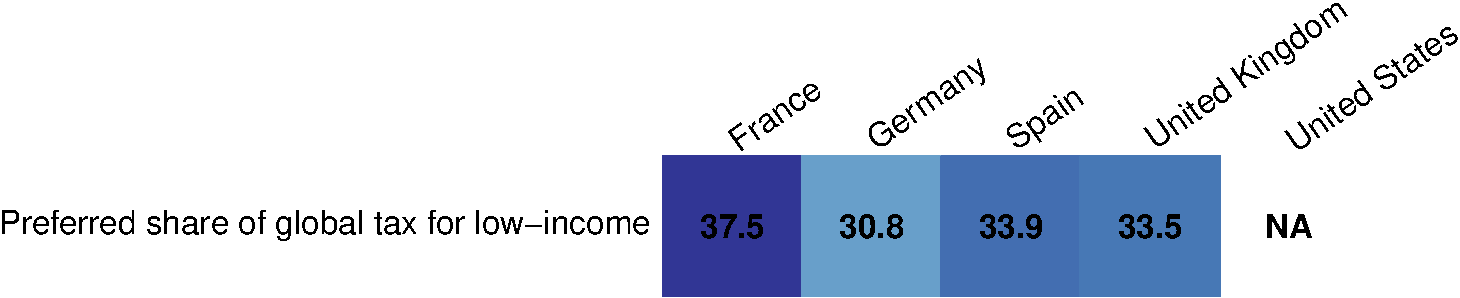
\includegraphics[width=1\textwidth]{../figures/country_comparison/global_tax_global_share_mean.pdf} \label{fig:global_share_mean}
% \end{figure}

% \setcounter{figure}{2}
% \renewcommand{\thefigure}{\arabic{figure}}
% \begin{figure}[h!]
%   % MAJOR figure
%   \caption[Relative support for other global policies]{Relative support for various global policies. (percentage of \textit{somewhat} or \textit{strong support}, after excluding \textit{indifferent} answers; *except for GCS: percentage of \textit{Yes} in a \textit{Yes}/\textit{No} question, preferred share: percentage of answers $\geq$30\%, and foreign aid: percentage of unconditional or conditional increase rather than decrease or stable aid). Shares of indifferent answers range from 10\% to 40\%, with quartiles 19\%, 25\%, and 32\%. (p. \pageref{subsec:questionnaire_GCS}, Questions \ref{q:gcs_support}, \ref{q:global_tax_global_share}, \ref{q:climate_policies}, \ref{q:other_policies}, and \ref{q:foreign_aid_raise_support}; See Figure \ref{fig:support_likert_positive} for the absolute support.)% $n_\text{US} = n_\text{Eu} = 3,000,\, n_\text{FR} = 729,\, n_\text{DE} = 929,\, n_\text{ES} = 543,\, n_\text{UK} = 749, n_\text{US, global/national wealth tax} = 2,000$
%   }
%   \makebox[\textwidth][c]{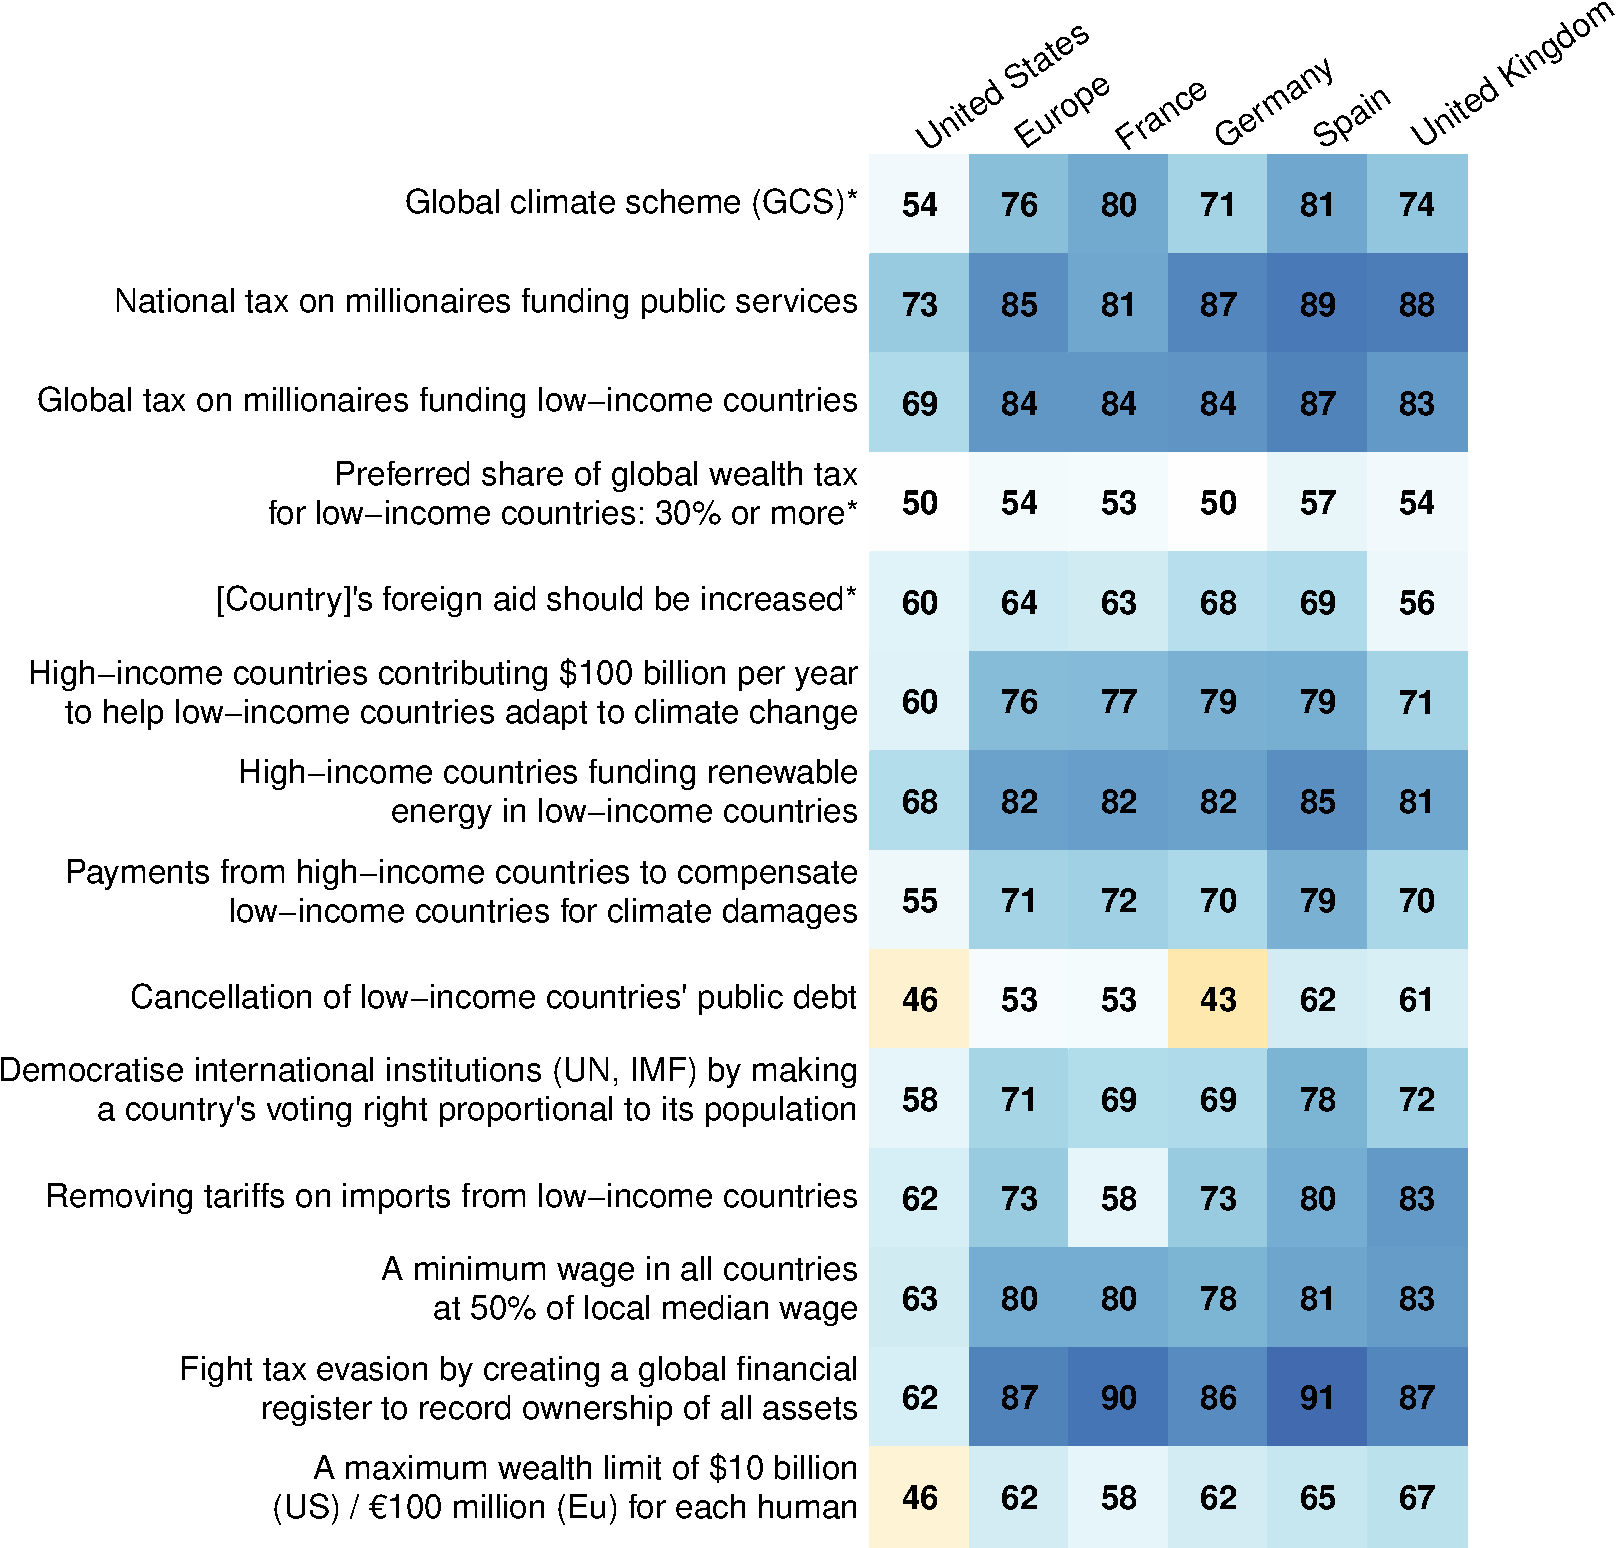
\includegraphics[width=\textwidth]{../figures/country_comparison/support_likert_all_share.pdf}}\label{fig:support}
% \end{figure} 
% \setcounter{figure}{5}
% \renewcommand{\thefigure}{S\arabic{figure}}
[Fig3] \refstepcounter{figure}\label{fig:support}

\subsubsection{Foreign aid}\label{subsubsec:support_foreign_aid} % NCCcomment
%\paragraph{Foreign aid}

In addition, we provide respondents with information about the actual amount ``spent on foreign aid to reduce poverty in low-income countries'' relative to their country's government spending and GDP. Less than 16\% of respondents state that their country's foreign aid should be reduced, while 62\% express support for increasing it, including 17\% who support an unconditional increase (Figure \ref{fig:foreign_aid_raise_support}). Among the 45\% who think aid should be increased under certain conditions, we subsequently ask them to specify the conditions they deem necessary (Figure \ref{fig:foreign_aid_condition}). The three most commonly selected conditions are that: ``we can be sure the aid reaches people in need and money is not diverted'' (73\% chose this condition), ``recipient countries comply with climate targets and human rights'' (67\%), and ``other high-income countries also increase their foreign aid'' (48\%). %\footnote{It is worth noting that these conditions align closely with the principles of the GCS.} 
On the other hand, respondents who do not wish to increase their country's foreign aid primarily justify their view by prioritizing the well-being of their fellow citizens or by perceiving each country as responsible for its own fate (Figure \ref{fig:foreign_aid_no}). In response to an open-ended question regarding measures high-income countries should take to fight extreme poverty, a large majority of Americans expressed that more help is needed (Suppl. Figure S39). % \ref{fig:poverty_field}). 
The most commonly suggested form of aid is financial support, closely followed by investments in education. 

% TODO? Explain the link between the two surveys blocks
We also inquire about the perceived amount of foreign aid. Consistent with prior research (see S.I. A.1.3), %Appendix \ref{subsubsec:literature_foreign_aid}), 
most people overestimate the actual amount of foreign aid (Suppl. Figure S18). % \ref{fig:foreign_aid_belief}). 
We then elicit respondents' preferred amount of foreign aid, after randomly presenting them with either the actual amount or no information. Most of the respondents who learn the actual amount choose a bracket at least as high as the actual one, and most of those without the information choose a bracket at least as high as the perceived one (Suppl. Figures S20-S21). %\ref{fig:foreign_aid_amount}--\ref{fig:foreign_aid_preferred_info}). 
Finally, we ask a last question to the respondents who received the information. To those who prefer an increase of foreign aid, we ask how they would finance it: by far, the preferred source of funding is higher taxes on the wealthiest (Suppl. Figure S23). %\ref{fig:foreign_aid_raise_how}). 
To those who prefer a reduction, we ask how they would use the funds becoming available: %resulting savings: 
In every country, more people choose higher spending on education or healthcare rather than lower taxes (Suppl. Figure S24). %\ref{fig:foreign_aid_reduce_how}). 


% \begin{tcolorbox}\label{subsec:universalistic}
%   \paragraph{Universalistic values}
\subsection{Universalistic values}\label{subsec:universalistic}
% H4: A strong majority is universalist/cosmopolitan (TODO: which word?), even a majority for non-Republican
% TD It is not obvious how these answers are informative of malleable opinions. So I don't think we should state the hypothesis and sell this as a test.
%Another hypothesis to explain the discrepancy between the lack of interest for global policies in the public debate despite a strong stated support is that opinions on the topic are weak and malleable. A way to test this is to

We ask broad questions on people's values to assess whether their core values are consistent with support for specific policies. 
% We elicit underlying values, to test whether broad values are consistent with people's support for specific policies. %To better understand people's support for specific policies, we also ask broad questions to study their values. %We ask broad questions on people's values to see whether their core values are consistent with universalism. 
% We also elicit underlying values, to test whether values are consistent with people's support for specific policies. Most people express some degree of universalism, consistently with the support for specific policies. 
When we ask respondents which group they defend when they vote, % ($n$ = 6,000)
20\% choose ``sentient beings (humans and animals),'' 22\% choose ``humans,'' 33\% select their ``fellow citizens'' (or ``Europeans''), 15\% choose ``My family and myself,'' and the remaining 9\% choose another group (mainly ``My State or region'' or ``People sharing my culture or religion''). 
% The first two categories, representing close to one out of two people, 
% can be described as universalist in their vote. 
Notably, a majority of left-wing voters choose \textit{humans} or \textit{sentient beings}. 
% are universalist in their vote (see Figure \ref{fig:main_by_vote}). % for main attitudes by vote).% The share of universalist even constitutes a majority of left-wing voters

Answers to this and other broad value questions are consistent with half of Americans and three quarters of Europeans supporting global policies like the GCS: people are almost as much willing to make a donation to poor Africans than to poor fellow citizens in a lottery experiment, most respondents find that global poverty and climate change are bigger problems than national inequality, and most respondents wish that their diplomats take into account global justice (see \nameref{sec:methods} for details).
%Regarding the priorities of their country's diplomats in international climate negotiations, 


% TODO! put back?
% Overall, answers to these broad value questions are consistent with half of Americans and three quarters of Europeans supporting global policies like the GCS: people are almost as much willing to give to poor Africans than to poor fellow citizens, find that global issues are among the biggest problems, almost half of them are universalist when they vote, and most of them wish that their diplomats take into account global justice.
% \end{tcolorbox}

% \begin{figure}[h!]
%   \caption[Attitudes on the evolution of foreign aid]{[For Supplementary Material] Attitudes regarding the evolution of [own country] foreign aid. (Question \ref{q:foreign_aid_raise_support})}\label{fig:foreign_aid_raise_support}
%   \makebox[\textwidth][c]{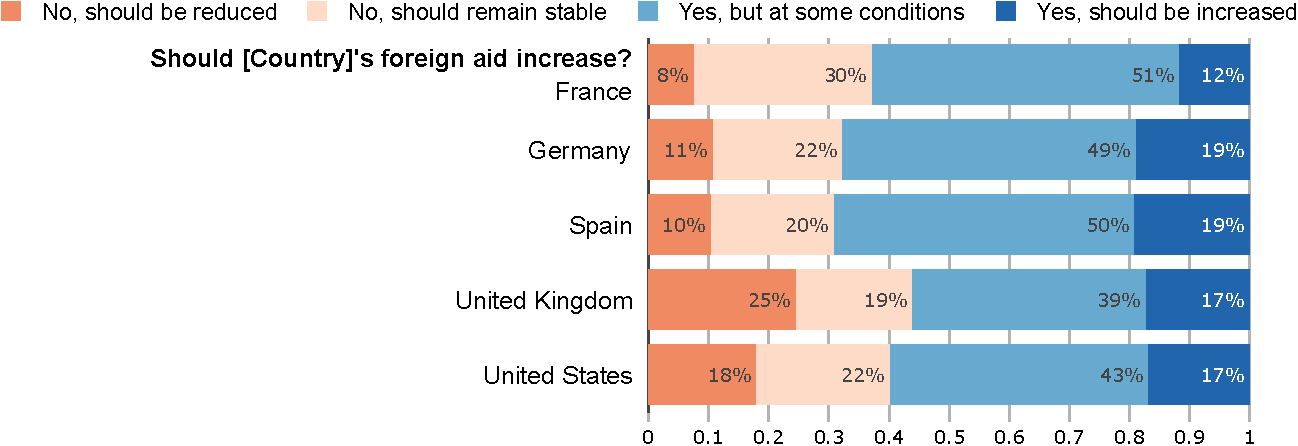
\includegraphics[width=\textwidth]{../figures/country_comparison/foreign_aid_raise_support.pdf}} 
% \end{figure}

% \begin{figure}[h!]
%   \caption[Conditions at which foreign aid should be increased]{[For Supplementary Material] Conditions at which foreign aid should be increased (in percent). [Asked to those who wish an increase of foreign aid at some conditions.] (Question \ref{q:foreign_aid_condition})}\label{fig:foreign_aid_condition}
%   \makebox[\textwidth][c]{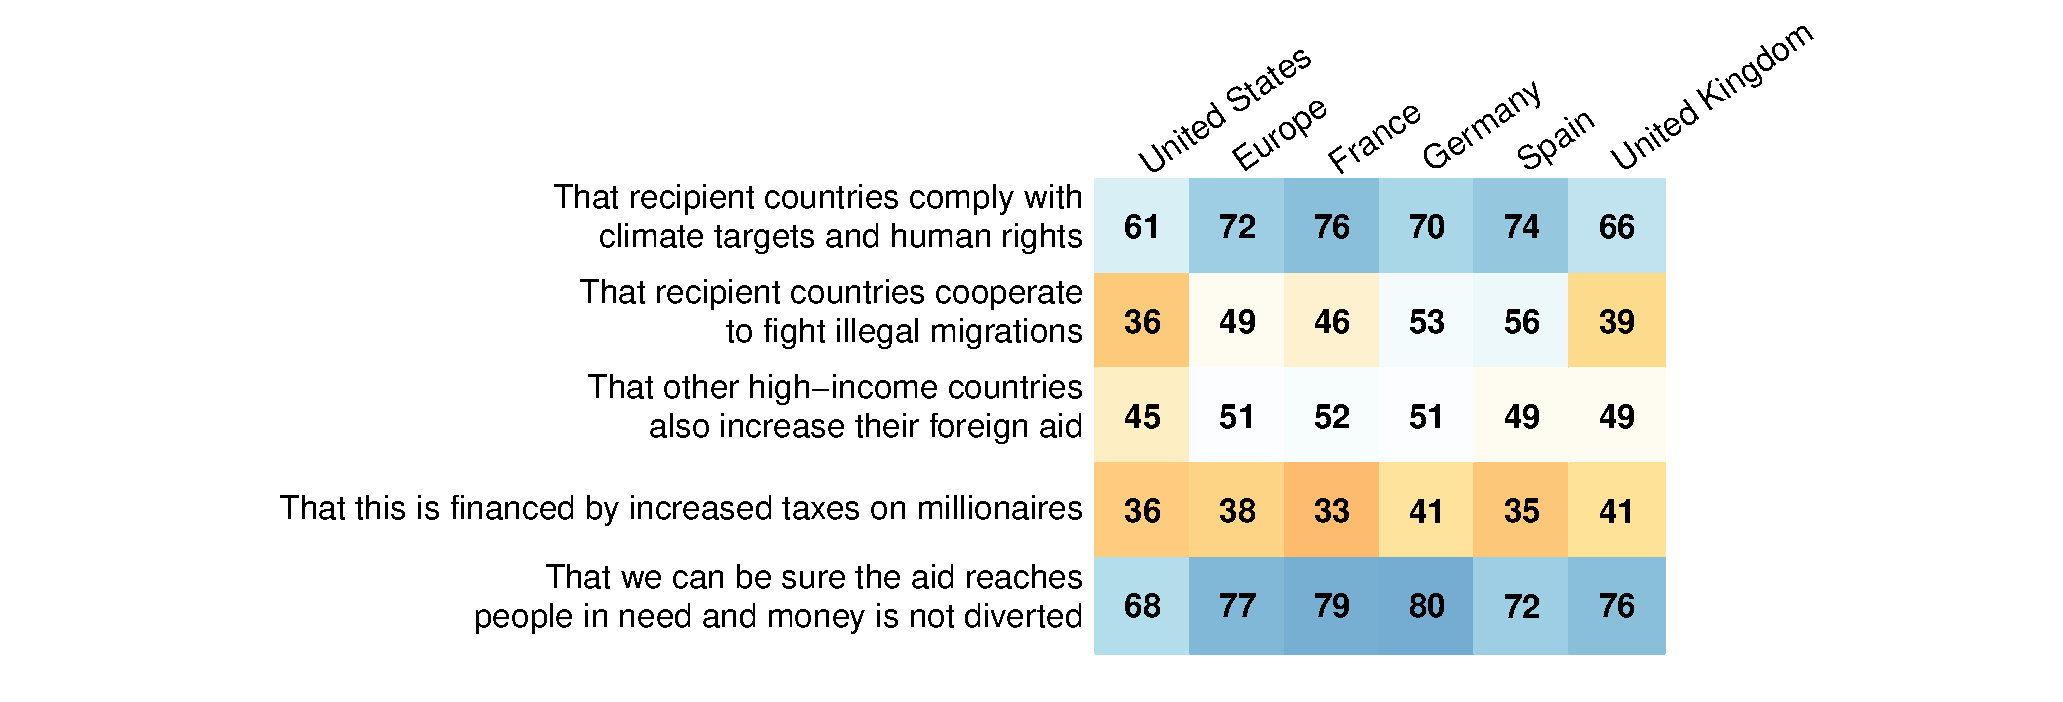
\includegraphics[width=\textwidth]{../figures/country_comparison/foreign_aid_condition_positive.pdf}} 
% \end{figure}

% \begin{figure}[h!]
%   \caption[Reasons why foreign aid should not be increased]{[For Supplementary Material] Reasons why foreign aid should not be increased (in percent). [Asked to those who wish a decrease or stability of foreign aid.] (Question \ref{q:foreign_aid_no})}\label{fig:foreign_aid_no}
%   \makebox[\textwidth][c]{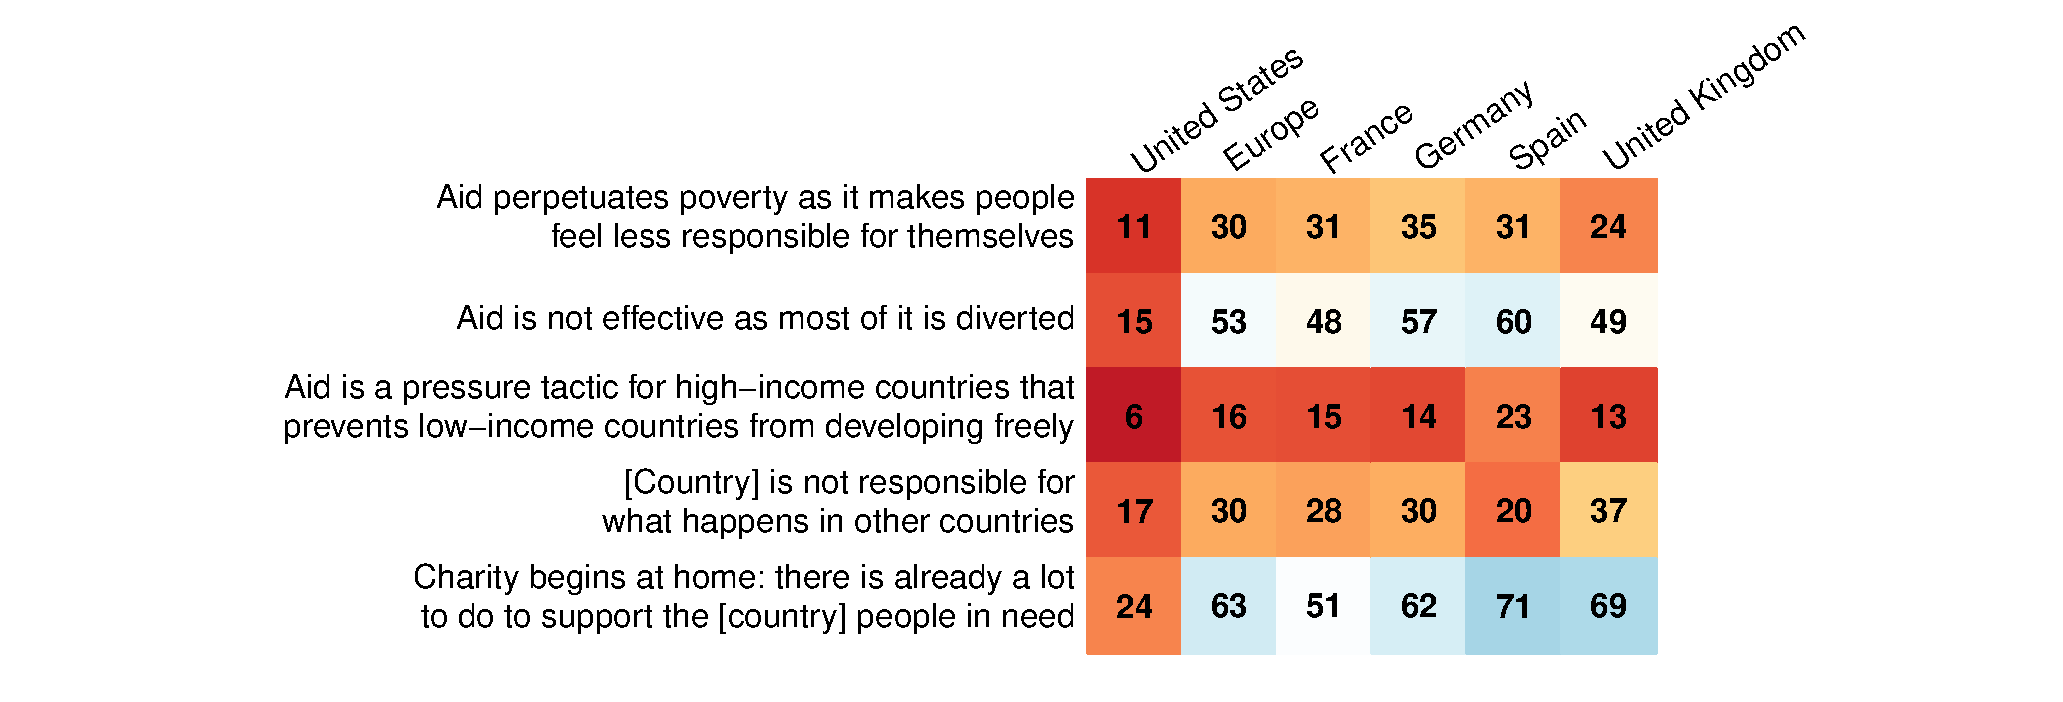
\includegraphics[width=\textwidth]{../figures/country_comparison/foreign_aid_no_positive.pdf}} 
% \end{figure}

\section{Discussion} % Summary, conclusion


% TODO? give less space to OECD paper?
% Our point of departure are recent surveys conducted %by \citet{dechezlepretre_fighting_nodate} 
% in 20 of the largest countries% \citep{dechezlepretre_fighting_nodate}
% , as they reveal strong majority support for global climate and redistributive policies, even in high-income countries that would financially lose from them.  In our main analysis, we find strong support for our main policy of interest --- the Global Climate Scheme (GCS) --- and for global taxes on the wealthiest individuals. The GCS encompasses carbon pricing at a global level through an emissions trading system, accompanied by a global basic income funded by the scheme's revenues. Additional experiments, such as a list experiment and a real-stake petition, confirm that the support for the GCS is real. 
% Such genuine support is further substantiated by the prioritization of the GCS over prominent national climate policies and aligned with a significant portion of the population holding universalistic values rather than nationalistic or egoistic ones. Moreover, the conjoint analyses indicate that a progressive candidate would not lose voting shares by endorsing the GCS, and may even gain 11 p.p. in voting shares in France. Similarly, a candidate endorsing the GCS would gain votes in a U.S. Democratic primary, while in Europe, a progressive platform that includes the GCS would be preferred over one that does not.

In our analysis, we have uncovered strong and genuine support for global redistributive policies. % One limitation to this finding, inherent to any inquiry into hypothetical policies, is that the support might change once global policies are discussed in the public debate (as explored in the paragraph on \textit{Pros and Cons}). 

We conclude by providing hypotheses to reconcile the scarcity of global policies in the public debate with our findings that they would be widely accepted. %As we ruled out all hypotheses of our registration plan,\footnote{The project was preregistered in the Open Science Foundation registry (\href{https://osf.io/fy6gd}{osf.io/fy6gd}).} we now need to study new explanations.
The first two are variations of pluralistic ignorance, and the last three represent complementary explanations. 

First, there may be pluralistic ignorance \textit{among policymakers} regarding universalistic values, support for the GCS, or the electoral advantage of endorsing it. 
Second, citizens or policymakers may believe that globally redistributive policies are politically infeasible in some key (potentially foreign) countries such as the U.S. % We intend to test these hypotheses by running a survey on Congress staffers and Members of the European Parliament.  %Second, there may be a more subtle form of pluralistic ignorance: although most people correctly predict what people would answer to a survey question, they may view globally redistributive policies as unrealistic, perhaps because they have never reflected upon the fact that many people across the world hold univeralistic values and are supportive of global solidarity. Third, most people and perhaps even most policy makers may have simply never heard of the GCS, let alone built their political ideas upon it. 
Third, political discourse centrally happens at the national level, shaped by national media and institutions such as the voting system. 
National framing by political voices may create biases and suppress universalistic values. % Third, most institutions are national: the largest scale votes take place at the national level% so political platforms are devised at this level, most media target a national audience, most commentators frame their discourse from a national perspective and portray relations to foreign countries as conflictual. 
Fourth, many individuals, including policymakers, may be unaware of specific proposals or may perceive global redistributive policies as ill-defined or technically infeasible, %or may , 
ultimately dismissing them as unrealistic. % In particular, policymakers may have insider information about the technical feasibility of such policies. Alternatively, the perception of unrealism may stem from an unawareness of specific proposals. % cautiously doubt that they are well-specified
% TODO? rewrite as a fifth hypothesis that the policies may indeed not be well specified nor implementable?
% Fourth, many individuals, including policymakers, may simply be unaware of specific global redistributive policies, let alone base their political ideas on them. This lack of awareness may lead people to % cautiously doubt that they are well-specified
% perceive such policies as ill-defined or technically infeasible, ultimately dismissing them as unrealistic. % TODO? rewrite as a fifth hypothesis that the policies may indeed not be well specified nor implementable?
% The latter hypothesis is supported by the prior ignorance of the GCS expressed in the feedback fields, where a common response is a variation of ``thank you for this interesting, thought-provoking survey.'' 
% TODO? remove?
Fifth, just as policy is disproportionately influenced by the economic elites,\citep{mccright_defeating_2003,gilens_testing_2014,persson_rich_2023} public debate may be shaped by the wealthiest, who have vested interests in preventing global redistribution.

% Also: vested interest influence on elites (a la Gilens and Page for the US, Persson & Sundell 23), cf. Boone story
% decline of support the more specific a measure gets / enters the public debate => addressed in conclusion of pros and cons
% people not believing that the policy is technically implementable => addressed
% politicians seeing defects or lack of specification of the policy that warrant opposition, while ignorant citizens would naively like it => addressed
% platform don't matter for vote

% LM This are all legtimiate and important points. For a global transfer (rather than say a EU transfer), I am really missing remarks about (lack) of quality of governance, rent creation and capture, corruption etc. To play devil's advocate, as much as I am sympathetic to the idea, I'm not sure I would currently vote in favor of such policies. Why? Not because I dislike the idea, but I am not sure that my carbon tax rent as a German would actually reach the poor population of Indonesia or Nigeria rather than the pockets of cleptocratic elites :) I'd like the draft to reflect that and could make an attempt to pre-empt that objection based on some references later in the project.
%In any case, 

Uncovering evidence to support the above hypotheses could draw attention to global policies in the public debate and contribute to their increased prominence. Their confirmation would further support the conclusion that there exists substantial public support for global policies addressing climate change and global inequality, even in high-income countries.
% Confirmation of any of these hypotheses would lead to a common conclusion: there exists substantial public support for global policies addressing climate change and global inequality, even in high-income countries. % despite the current perceived boundaries of political realism on them. % on this issue may soon shift. %Recent developments suggest that such a change might be underway: the \citet{african_union_african_2023} calls for a global carbon taxation regime, a call quickly endorsed by the President of the EU Commission;\footnote{Cf. this tweet by Ursula von der Leyen: \href{https://twitter.com/vonderleyen/status/1700416700238225659}{twitter.com/vonderleyen/status/1700416700238225659}.} the \citet{un_promotion_2023} is setting up a Framework Convention on International Tax Cooperation, where various countries want to open discussions about a global wealth tax; Brazil uses its presidency of the G20 in 2024 to propose a global tax to finance sustainable development; the International Maritime Organization is poised to adopt a global carbon levy on maritime fuel; etc. 
% Uncovering evidence to support the above hypotheses could shift the perceived boundaries of political realism on this issue. %help TODO this one?
% draw attention to global policies in the public debate and contribute to their increased prominence. % Uncovering evidence for this might actually contribute itself to garner more attention to global policies in the public debate. 

% Also: no short term outcome (before the end of the mandate) so no incentive to start it

% TODO!? alternative conclusion: strong and sincere support for global wealth tax in both continents => probable reason why it's not more discussed is that it's not the determining issue for voters. Strong and sincere support for the GCS in Europe but half-half in the U.S. (where there is a risk that support decreases in a campaign) => not endorsed by the Democrats because they seek policies more strongly supported, and not discussed in Europe probably because the U.S. won't support it.

% For warm glow and how to test it, see my 28/6, 30/6,  (2023) emails (elicit beliefs on feasibility/obstacles, ask support for Bridgetown / 100G€ with vs. without saying it may be approved at the COP, redo conjoint analysis without support question before, asking for approval of global redistr. policy costing 50€/month with/without asking for a similar one costing 20€/month before). 
% For new survey, also test one ambitious (no one with less than 7$/day), unilateral global wealth tax and GCP with partial participation

% \begin{methods}  % WPcomment
  \begin{small} % NCCcomment
%Put methods in here.  If you are going to subsection it, use \subsection commands.  Methods section should be less than 800 words and if it is less than 200 words, it can be incorporated into the main text.
\section*{\normalsize Methods}\label{sec:methods} % NCCcomment
\addcontentsline{toc}{section}{\nameref{sec:methods}}

\paragraph{\small Pre-registration.}
The project is approved by Economics \& Business Ethics Committee (EBEC) at the University of Amsterdam (EB-1113) and %is approved by IRB at Harvard University (IRB21-0137), and 
was preregistered in the Open Science Foundation registry on January 10, 2023 (\href{https://osf.io/fy6gd}{osf.io/fy6gd}). The study did not deviate from the registration: the questionnaires and the hypotheses tests used are the same as the ones \href{https://osf.io/2b6vq}{given \textit{ex ante}}. Informed consent was obtained from all respondents, randomized treatment branches were unkown to the respondents, and our research complies with all relevant ethical regulations. Respondents were compensated with gift certificates for a value of \euro{}1 after participation. No statistical methods were used to pre-determine sample sizes but our sample sizes match those reported in similar publications.\citep{dechezlepretre_fighting_nodate,issp_international_2010,beiser-mcgrath_could_2019,sivonen_attitudes_2022,douenne_yellow_2022}
% \subsection{Data collection.} % WPcomment

\paragraph{\small Data collection.} % NCCcomment
% The paper relies on two different sets of surveys. The first set of surveys was conducted between March 2021 and March 2022 on 40,680 respondents from 20 countries  (between 1,465 and 2,488 respondents per country). The first U.S. complementary, denoted \textit{US1}, was conducted on 3,000 U.S. respondents between January and March 2023, while the second, \textit{US2}, was conducted on 2,000 respondents between March and April 2023. The \textit{Eu} complementary survey was conducted on 3,000 respondents between February and March 2023. We used the survey companies \emph{Dynata} and \emph{Respondi}. Stratified quotas ensure that the samples are representative along the dimensions of gender, age (5 brackets), income (4), region (4), education level (3), as well as ethnicity (3) for the U.S. To correct for small remaining imbalances, we apply survey weights throughout the analysis, constructed using the quotas variables as well as the degree of urbanity, and trimmed between 0.25 and 4. Weights make the results fully representative of the country (or of the four European countries combined in the case of results at the European level, where different weights are used). Appendix \ref{app:representativeness} confirms that our samples are representative of the population. % TODO! and urbanity instead of education for OECD, TODO table representativeness
%\footnote{We trim weights so that no respondent receives a weight below 0.25 or above 4. Overall, trimming changes the weights for xx\% of the respondents.} 

The paper utilizes two sets of surveys (with blinding): the \textit{global} survey and the \textit{Western} surveys. The \textit{global} surveys consist of two U.S. surveys, \textit{US1} and \textit{US2}, and one European survey, \textit{Eu}. The \textit{global} survey was conducted from March 2021 to March 2022 on 40,680 respondents from 20 countries (with 1,465 to 2,488 respondents per country). \textit{US1} collected responses from 3,000 respondents between January and March 2023, while \textit{US2} gathered data from 2,000 respondents between March and April 2023. \textit{Eu} included 3,000 respondents and was conducted from February to March 2023. We used the survey companies \emph{Dynata} and \emph{Bilendi}. To ensure representative samples, we employed stratified quotas based on gender, age (5 brackets), income (4), region (4), education level (3), and ethnicity (3) for the U.S. We also incorporated survey weights throughout the analysis to account for any remaining imbalances. These weights were constructed using the quota variables as well as the degree of urbanization, and trimmed between 0.25 and 4. Stratified quotas followed by reweighting is the usual method to reduce selection bias from opt-in online panels, when better sampling methods (such as compulsory participation of random dwellings) are unavailable.\cite{scherpenzeel_how_2010} By applying weights, the results are fully representative of the respective countries along the above mentioned dimensions. %. 
Results at the European level apply different weights which ensure  representativeness of the combined four European countries. 
% Appendix \ref{app:representativeness} 
S.I. G 
shows how our samples compare to actual population frequencies. They match the actual frequencies, except for some imbalances in specific quota demographics ---such as gender in the UK (43\% of women instead of 50\%) or urbanity in Spain (15\% rural instead of 26\%)--- that are corrected through our survey weights, and in the U.S. vote (which does not affect our results, as shown by the results reweighted by vote in the \textit{Support for the GCS} section below). 
% confirms that our samples are representative of the population. %\footnote{We trim weights so that no respondent receives a weight below 0.25 or above 4. Overall, trimming changes the weights for xx\% of the respondents.} 
% TODO? that our samples closely match population frequencies in high-income countries. In middle-income countries, the samples are only representative of the online population (young, graduated and urban people are over-represented).
% Appendix \ref{app:balance} 
S.I. I 
shows that the treatment branches are balanced. 
% Appendix \ref{app:placebo} 
S.I. J 
runs placebo tests of the effects of each treatment on unrelated outcomes. We do not find effects of earlier treatments on unrelated outcomes arriving later in the survey. 
% Appendix \ref{app:extended} 


% \subsection*{\small Data quality.} % WPcomment % TODO attrition analysis
\paragraph{\small Data quality.} % NCCcomment
The median duration is 28 minutes for the \textit{global} survey, 14 min for \textit{US1}, 11 min for \textit{US2}, and 20 min for \textit{Eu}. To ensure the best possible data quality, we exclude 14\% inattentive respondents who fail an attention test or rush through the survey (i.e., answer in less than 11.5 minutes in the \textit{global} survey, 4 minutes in \textit{US1} or \textit{US2}, 6 minutes in \textit{Eu}). Indeed, responses of excluded respondents may be unreliable. S.I. K 
shows that our results are unchanged when including inattentive respondents. %All the results and analyses use survey weights, defined to make the results fully representative of the country (or of Eu in the case of results at the Eu level) along the quota variables. Weights are trimmed to be between .25 and 4. 
%\textit{Ex post}, we checked that there were only a few careless response patterns (such as choosing the same answer for all items in a matrix of questions; see Appendix \ref{app:data_quality}). 
At the end of the survey, we ask whether respondents thought that our survey was politically biased and offer to provide some feedback. 69\% of the respondents found the survey unbiased. 24\% found it left-wing biased, and 8\% found it right-wing biased.

\paragraph{\small Statistical tests.}
All t-tests are two-tailed and without adjustment for multiple comparisons. Tables report 95\% confidence intervals. 

% \subsection*{\small Questionnaires and raw results.} % WPcomment
\paragraph{\small Questionnaires and raw results.} % NCCcomment
% Possible confusion in the questionnaire: people confuse GCS with the four policies together (so support for GCS can suffer from dislike of death penalty), although this confusion is mitigating by the fact that we right after ask about NR; people may answer about revenue-use rather than the whole measure for ETS2 support; people may answer that GCS will or will not have the effects proposed rather than these effects being important or not in their attitude towards GCS; they may answer that it's important that others (not them) get more information; the minimum wage could be reduced at 50% of local median wage.
%.\cite{dechezlepretre_fighting_nodate} 
The raw results are reported in S.I. B % Appendix \ref{app:raw_results} 
while the surveys' structures and questionnaires are given in S.I. C and D. % Appendices \ref{app:questionnaire_oecd} and \ref{app:questionnaire}. 
Details on the \textit{global} survey can be found in the Appendix of Dechezleprêtre et al. (forthcoming).\citep{dechezlepretre_fighting_nodate} Country-specific raw results are also available as supplementary material files:  \href{https://github.com/bixiou/international_attitudes_toward_global_policies/raw/main/paper/app_desc_stats_US.pdf}{US}, \href{https://github.com/bixiou/international_attitudes_toward_global_policies/raw/main/paper/app_desc_stats_EU.pdf}{EU}, \href{https://github.com/bixiou/international_attitudes_toward_global_policies/raw/main/paper/app_desc_stats_FR.pdf}{FR}, \href{https://github.com/bixiou/international_attitudes_toward_global_policies/raw/main/paper/app_desc_stats_DE.pdf}{DE}, \href{https://github.com/bixiou/international_attitudes_toward_global_policies/raw/main/paper/app_desc_stats_ES.pdf}{ES}, \href{https://github.com/bixiou/international_attitudes_toward_global_policies/raw/main/paper/app_desc_stats_UK.pdf}{UK}. %The questionnaires are the same as the ones given \textit{ex ante} in the registration plan (\href{https://osf.io/fy6gd}{osf.io/fy6gd}).


% \subsection*{\small Incentives.} % WPcomment
\paragraph{\small Incentives.} % NCCcomment
To encourage accurate and truthful responses, several questions of the Western surveys use incentives. For each of the three comprehension questions that follow the policy descriptions, we randomly select and reward three respondents who provide correct answers with a \$50 gift certificate. Similarly, for questions involving estimating support shares for the GCS and NR, three respondents with the closest guesses to the actual values receive a \$50 gift certificate. In the donation lottery question, we randomly select one respondent and split the \$100 prize between the NGO GiveDirectly and the winner according to the winner's choice. In total, our incentives scheme distributes gift certificates (and donations) for a value of \$850. Finally, respondents have an incentive to answer truthfully to the petition question, as they are aware that the results for that question (the share of respondents supporting the policy) will be transmitted to the office of their head of state.

%To encourage respondents to answer accurately and truthfully, several questions of the \textit{US1} survey use incentives. For each of the three comprehension questions that follow the policies' descriptions, we reward three (randomly drawn) respondents with the correct answer with a \$50 gift certificate. For each of the questions asking respondents to guess the share of support for the GCS and NR, we reward three people who are closest to the true value with a \$50 gift certificate. For the donation lottery question, we randomly draw one respondent and split the \$100 prize between the NGO GiveDirectly and the winner according to the winner's choice. In total, our incentives scheme distributes gift certificates (and donation) for a value of \$850. Finally, respondents have an incentive to answer truthfully to the petition question, given that they know that the results to that question (the share of respondents supporting the policy) will be transmitted to the U.S. President's office.

\paragraph{\small Absolute vs. relative support.}
In most questions, support or opposition for a policy is asked using a 5-Likert scale, with compulsory response and \textit{Indifferent} as the middle option. We call \textit{absolute support} the share of \textit{Somewhat} or \textit{Strong support}. We generally favor the notion of \textit{relative support}, which reports the share of support after excluding \textit{Indifferent} answers. Indeed, the \textit{relative support} is better suited to assess whether there are more people in favor vs. against a policy.

\paragraph{\small Support for the GCS.} 
The 95\% confidence intervals are $[52.4\%, 56.0\%]$ in the U.S. and $[74.2\%, 77.2\%]$ in Europe. The average support is computed with survey weights, employing weights based on quota variables, which exclude vote. Another method to reweigh the raw results involves running a regression of the support for the GCS on sociodemographic characteristics (including vote) and multiplying each coefficient by the population frequencies. This alternative approach yields similar figures: 76\% in Europe and 52\% or 53\% in the U.S. (depending on whether individuals who did not disclose their vote are classified as non-voters or excluded). The average support among voters is 54\% in the U.S., with 74\% support among Biden voters vs. 26\% among Trump voters (see Suppl. Figure S40). % \ref{fig:main_by_vote}).

Though the level of support for the GCS is significantly lower in swing States (at 51\%) that are key to win U.S. elections, the electoral effect of endorsing the GCS remains non-significantly different from zero (at +1.2 p.p.) in these States. Note that we define swing states as the 8 states with less than 5 p.p. margin of victory in the 2020 election (MI, NV, PA, WI, AZ, GA, NC, FL). The results are unchanged if we use the 3 p.p. threshold (that excludes FL) instead. 

\paragraph{\small List experiment.} % TODO! report Bayes Factors or equivalence tests for the null result
List experiments have been used to reveal social desirability bias, silencing either racism in the Southern U.S.\citep{kuklinski_racial_1997} or opposition to the invasion of Ukraine in Russia.\citep{chapkovski_solid_2022} % TODO? remove?
In our case, the question reads: ``Beware, this question is quite unusual. Among the policies below, \textbf{how many} do you support?'' The list of policies randomly varies across respondents, and includes a subset of GCS, NR (National Redistribution scheme), C (``Coal exit'' in the U.S., ``Thermal insulation plan'' in Europe) and O (``Marriage only for opposite-sex couples in the U.S.'', ``Death penalty for major crimes'' in Europe). There are four branches: GCS/NR/C/O; GCS/C/O; NR/C/O; C/O. To estimate the tacit average support for the GCS and NR, we regress the number of supported policies on indicators that the list includes GCS and NR.
We utilize the difference-in-means estimator, and confidence intervals are computed using Monte Carlo simulation with the R package \textit{list}.\citep{imai_multivariate_2011}

\paragraph{\small Petition.}
The respondent is randomly assigned a branch where the petition relates to the GCS or the National Redistribution scheme. The question reads: ``Would you be willing to sign a petition for the [Global climate / National redistribution] scheme? \\ As soon as the survey is complete, we will send the results to [the U.S. President's office], informing him what share of [American] people are willing to endorse the [Global climate / National redistribution] scheme. (You will NOT be asked to sign, only your answer here is required and remains anonymous.)''. 

Paired weighted \textit{t}-tests are conducted to test the equality in support for a policy among respondents who were questioned about the policy in the petition. 

\paragraph{\small Conjoint analyses.}
The first conjoint analysis suggests that the GCS is supported independently of being complemented by the National Redistribution Scheme and a national climate policy (``Coal exit'' in the U.S., ``Thermal insulation plan'' in Europe, denoted C). Indeed, 55\% of %($n$ = 3,000) 
U.S. respondents and 74\% of %($n$ = 3,000) 
European ones prefer the combination of C, NR and the GCS to the combination of C and NR alone, indicating similar support for the GCS conditional on NR and C than for the GCS alone (Suppl. Figure S8). %\ref{fig:conjoint}). 

In the second conjoint analysis, results from the first branch show that the support for the GCS conditional on NR, at 55\% in the U.S. ($n$ = 757) and 77\% in Europe ($n$ = 746), is not significantly different from the support for the GCS alone. This suggests that rejection of the GCS is not driven by the cost of the policy on oneself. The second branch indicates that the GCS, C, or their combination, are all similarly supported. This branch shows that the support for C conditional on NR is somewhat higher than the support for the GCS, at 62\% in the U.S. ($n$ = 751) and 84\% in Europe ($n$ = 747). However, the third one shows no significant preference for C compared to GCS (both conditional on NR), neither in Europe, where GCS is preferred by 52\% ($n$ = 741) nor in the U.S., where C is preferred by 53\% ($n$ = 721). The fourth branch shows that 55\% in the U.S. ($n$ = 771) and 77\% in Europe ($n$ = 766) prefer the combination of C, NR and the GCS to NR alone.

The effects reported in the fourth analysis are the Average Marginal Component Effects.\cite{hainmueller_causal_2014} The policies studied are progressive policies prominent in the country. Except for the category \textit{foreign policy}, which features the GCS 42\% of the time, they are drawn uniformly.

The results from the fourth and fifth analyses, suggesting an electoral advantage for candidates who support global policies, relate to the finding by Ghassim (2020) that 12\% of Germans shift their voting intention from SPD and CDU/CSU to the Greens and the Left when they are told that the latter parties support global democracy.\citep{ghassim_who_2020}


\paragraph{\small Prioritization.}
The prioritization allows inferring individual-level preferences for one policy over another, including their intensity. This somewhat differs from a conjoint analysis, which only allows inferring individual-level preferences for one platform over another or collective-level preferences for one policy over another. Also, by comparing platforms, conjoint analyses may be subject to interaction effects between policies of a platform (which can be seen as complementary, substitute, or antagonistic) while the prioritization frames the policies as independent.

This question sheds light on a potential discrepancy between the policy priorities of the public and those enacted by legislators. For instance, while the European Union and California have enacted plans to phase out new combustion-engine cars by 2035, the proposal to ``ban the sale of new combustion-engine cars by 2030'' emerged as one of the three least prioritized policies in each country, with an average allocation of 7.8 points in France to 11.4 points in the UK.

\paragraph{\small Open-ended question on the GCS.}
Around one in four respondents explicitly cites pros or cons. Few individuals explicitly express support or opposition, and misunderstandings are rare. Only 11\% of the responses are empty or express a lack of opinion, though one-quarter are unclassifiable due to the rarity, nonsensical nature, or irrelevance of the conveyed idea.

\paragraph{\small Pros and cons.}
In the closed question, the least important aspect was the negative impact on their household, with 60\% in Europe ($n$=1,505) and 75\% in the U.S. ($n$=493) finding it important. The most important elements differ between Europe and the U.S. In Europe, the key factors are the GCS's potential to limit climate change and reduce poverty in low-income countries, both deemed important by 85\% of respondents. In the U.S., having sufficient information about the scheme ranks highest at 89\%, followed by its potential to foster global cooperation at 82\%. 

Surprisingly, the support for National Redistribution also decreased by 7 p.p. following the closed question about the GCS. This suggests that some individuals may lack attention and confuse the two policies, or that contemplating the pros and cons alters the mood of some people, moving them away from their initial positive impression.

\paragraph{\small Universalistic values.}
When asked what their country's diplomats should defend in international climate negotiations, only 11\% prefer their country's ``interests, even if it goes against global justice.'' In contrast, 30\% prefer global justice (with or without consideration of national interests), and the bulk of respondents (38\%) prefer their country's ``interests, to the extent it respects global justice.''

Furthermore, when we ask respondents to assess the extent to which climate change, global poverty, and inequality in their country are problems, climate change is generally seen as the most important problem % , followed by global poverty and national inequality.
(with a mean score of 0.58 after recoding answers between $-$2 and 2). This is followed by global poverty (0.40) and national inequality (0.35). %, $n$ = 6,000).

Finally, we conduct a lottery experiment. % to elicit. % universalistic values. 
Respondents were automatically enrolled in a lottery with a \$100 prize and had to choose the proportion of the prize they would keep for themselves versus give to a person living in poverty. The % Finally, we created a lottery, where respondents choose the proportion of the \$100 prize they would keep for themselves versus give to a person living in poverty. The 
charity donation is directed either to an African individual or a fellow citizen, depending on the respondent's random assignment. In Europe, we observe no significant variation in the willingness to donate based on the recipient's origin (in line with an earlier study\cite{cappelen_needs_2013}). In the U.S., the donations to Africans are 3 p.p. lower, %(with an average donation of 34\%), 
but the slightly lower donations to Africans are entirely driven by Trump voters and non-voters (Table \ref{tab:donation}).

\paragraph{\small Global wealth tax estimates.}
A 2\% tax on net wealth exceeding \$5 million would annually raise \$816 billion, leaving 99.9\% of the world population untaxed. More specifically, it would collect \euro{}5 billion in Spain, \euro{}16 billion in France, £20 billion in the UK, \euro{}44 billion in Germany, \$430 billion in the U.S., and \$1 billion collectively in all low-income countries (28 countries, home to 700 million people). These Figures come from Kappeler et al. (2021)\cite{kapeller_european_2021} (for European countries) and the \href{https://wid.world/world-wealth-tax-simulator/}{WID wealth tax simulator} (for the U.S. and low-income countries).\cite{chancel_world_2022}

% \paragraph{\small Swing states.}
% We define swing states as the 8 states with less than 5 p.p. margin of victory in the 2020 election (MI, NV, PA, WI, AZ, GA, NC, FL). The results are robust to using the 3 p.p. threshold (that excludes FL) instead.
% Here is a description of a specific method used.  Note that the subsection heading ends with a full stop (period) and that the command is \verb|\subsection{}| not \verb|\subsection**{}|.

\paragraph{\small Design choices.}

As global survey results indicated strong support for global redistributive policies worldwide, we conducted our Western surveys to further investigate the surprisingly high support.  %We selected five high-income countries based on their size and their level of support for global redistributive policies observed in the Global survey. 
Among the eight largest high-income countries, we selected the five ones with a relatively low level of support for global redistributive policies as observed in the global survey. We also focus on the GCS as its costs are less concentrated on the very rich, compared to other global redistributive policies, so we expected lower (or less genuine) support. By selecting countries that would lose from global redistribution, are less supportive than others, and focusing on less consensual policies, we aimed at conservatively assessing the level of support of world citizens for global redistribution. 

We split the U.S. survey into two waves to test the effect on the support of providing the information on the actual support, and merged the \textit{Eu} survey in one wave to get larger sample sizes and more power in the analyses. 

To select the policies tested, we spanned three key areas for global redistribution: climate change, inequality, and global governance. We selected policies that are either on the agenda of international negotiations (international transfers for mitigation; adaptation; or loss and damages; cancellation of public debt; reform of voting rights at the UN or IMF; global wealth tax) or advocated by prominent NGOs or scholars (\href{https://static1.squarespace.com/static/5a0c602bf43b5594845abb81/t/5c988368eef1a1538c2ae7eb/1553498989927/GAR.pdf}{global asset registry}; limits on wealth;\citep{robeyns_limitarianism_2024,piketty_brief_2022} democratic climate governance;\citep{dryzek_global_2011} global minimum wage;\citep{palley_financial_2013} fair trade;\citep{hickel_divide_2017} carbon pricing;\citep{cramton_global_2017} \href{https://concordeurope.org/wp-content/uploads/2019/11/CONCORD_AidWatch_Report_2019_web.pdf}{increased foreign aid}).



\section*{\normalsize Data availability}

All data as well as figures of the paper are available on \href{https://github.com/bixiou/international_attitudes_toward_global_policies}{github.com/bixiou/international\_attitudes\_toward\_global\_policies}. 
% Data for the \textit{global} survey will be made public upon publication. % 

\section*{\normalsize Code availability}

The paper's replication requires R and RStudio (R 4.3.1, RStudio 2024.04.1 were used). All code is available on \href{https://zenodo.org/doi/10.5281/zenodo.11202245}{10.5281/zenodo.11202245} and \href{https://github.com/bixiou/international_attitudes_toward_global_policies}{github.com/bixiou/international\_attitudes\_toward\_global\_policies}. %\\ \href{https://github.com/bixiou/international_attitudes_toward_global_policies}{github.com/bixiou/global\_tax\_attitudes}. 
% Code for the \textit{global} survey will be made public upon publication. % 

\section*{\normalsize Acknowledgements}

We are grateful for financial support from A Sustainable Future (ASF) at the University of Amsterdam, and TU Berlin. L.M. also thanks the Robert Bosch Foundation. A.F. received funding from the Agence Nationale de la Recherche (ANR-24-CE03-7110). %We are grateful for financial support from the OECD, the French Ministry of Foreign Affairs, the French Conseil d’Analyse Economique and the Spanish Ministry for the Ecological Transition and Demographic Challenge. We also acknowledge support from the Grantham Foundation for the Protection of the Environment and the Economic and Social Research Council through the Centre for Climate Change Economics and Policy. 
We thank Antoine Dechezleprêtre, Tobias Kruse, Bluebery Planterose, Ana Sanchez Chico, and Stefanie Stantcheva for their invaluable inputs for the project. We thank Auriane Meilland for feedback. We are grateful to Rafael Wildauer for graciously providing estimates on wealth tax revenues. %We further thank Jakob Niemann, Laura Schepp, Martín Fernández-Sánchez, Samuel Gervais, Samuel Haddad, and Guadalupe Manzo for assistance. Fabre declares that he also serves as president of Global Redistribution Advocates. % TODO! put back

\section*{\normalsize Author Contributions} A.F. collected and analysed the data, and drafted the questionnaire and the paper. T.D. and L.M. substantially revised the questionnaire and paper, and contributed to the conception and redaction.

\section*{\normalsize Competing interests} Fabre declares that he also serves as treasurer of Global Redistribution Advocates. The remaining authors declare no competing interests. % TODO!? maintain?

% TODO! Tables and Figures legend here

% TODO!! Figures must be uploaded individually, one figure per file.


% \end{methods} % WPcomment
\end{small}  % NCCcomment

\begin{table}[h]
  % MAJOR figure % TODO! same table for NR in appendix
  % TODO table by country
  \caption[List experiment: tacit support for the GCS]{Number of supported policies in the list experiment depending on the presence of the Global Climate Scheme (GCS) in the list. %in function of the composition of the list. GCS stands for the Global Climate Scheme and NR for the National Redistribution Scheme.} % Beware, this question is quite unusual. \\ Among the policies below, how many do you support?  \\ Coal exit, Marriage only for opposite-sex couples 
   The tacit support for the GCS is estimated by regressing the number of supported policies on the presence of the GCS in the list of policies. The social desirability is estimated as the difference-in-means between the tacit and stated support (see \nameref{sec:methods}), and it is not significantly different from zero even at a 20\% threshold (as shown by the 80\% Confidence Interval). 
  }\label{tab:list_exp}
  \makebox[\textwidth][c]{
\begin{tabular}{@{\extracolsep{5pt}}lccc} 
\\[-1.8ex]\hline 
\hline \\[-1.8ex] 
 & \multicolumn{3}{c}{Number of supported policies} \\ 
\cline{2-4} 
\\[-1.8ex] & All & U.S. & Europe \\ 
\hline \\[-1.8ex] 
 List contains: GCS & 0.624 & 0.524 & 0.724 \\ 
  & (P $<$ 0.001) & (P $<$ 0.001) & (P $<$ 0.001) \\ 
\hline  \\[-1.8ex] \textit{Support for GCS} & 0.65  &  0.542  &  0.757 \\
\textit{Social desirability bias} & \textit{$ -0.026 $} & \textit{$ -0.018 $} & \textit{$ -0.033 $}\\
\textit{80\% C.I. for the bias} & \textit{ $[ -0.06 ; 0.01 ]$ } & \textit{ $[ -0.07 ; 0.04 ]$} & \textit{ $[ -0.08 ; 0.01 ]$}\\
 \hline \\[-1.8ex] 
Constant & 1.317 & 1.147 & 1.486 \\ 
Observations & 6,000 & 3,000 & 3,000 \\ 
R$^{2}$ & 0.089 & 0.065 & 0.125 \\ 
\hline 
\hline \\[-1.8ex] 
\end{tabular} 
  %
\begin{tabular}{@{\extracolsep{5pt}}lccc} 
\\[-1.8ex]\hline 
\hline \\[-1.8ex] 
 & \multicolumn{3}{c}{Number of supported policies} \\ 
\cline{2-4} 
\\[-1.8ex] & All & US & Europe \\ 
\hline \\[-1.8ex] 
 List contains: GCS & 0.624$^{***}$ & 0.524$^{***}$ & 0.724$^{***}$ \\ 
  & (0.028) & (0.041) & (0.036) \\ 
\hline  \\[-1.8ex] \textit{Support for GCS} & 0.65  &  0.542  &  0.757 \\
\textit{Social desirability bias} & \textit{$ -0.026 $} & \textit{$ -0.018 $} & \textit{$ -0.033 $}\\
\textit{80\% C.I. for the bias} & \textit{ $[ -0.06 ; 0.01 ]$ } & \textit{ $[ -0.07 ; 0.01 ]$} & \textit{ $[ -0.08 ; 0.01 ]$}\\
 \hline \\[-1.8ex] 
Constant & 1.317 & 1.147 & 1.486 \\ 
Observations & 6,000 & 3,000 & 3,000 \\ 
R$^{2}$ & 0.089 & 0.065 & 0.125 \\ 
\hline 
\hline \\[-1.8ex] 
\textit{Note:}  & \multicolumn{3}{r}{$^{*}$p$<$0.1; $^{**}$p$<$0.05; $^{***}$p$<$0.01} \\ 
\end{tabular} 
  }  
  % {\footnotesize \textit{Note:} $^{*}p<0.1$; $^{**} p<0.05$; $^{***} p<0.01$.}
\end{table}

\begin{table}[h]
  % MAJOR figure
  \caption[Influence of the GCS on electoral prospects]{Preference for a progressive platform depending on whether it includes the GCS or not. (Question 28) %\ref{q:conjoint_c}) 
  %Imagine if the [Democratic and Republican presidential candidates in 2024] campaigned with the following policies in their platforms. [Credible Progressive and Conservative platforms] \\ % TODO See More
% Which of these candidates would you vote for? \textit{A; B; None of them} \\
% ~[FR: second round of presidential; DE, ES, UK: two favorite candidates in one's constituency]
} % Beware, this question is quite unusual. \\ Among the policies below, how many do you support?  \\ Coal exit, Marriage only for opposite-sex couples 
  \makebox[\textwidth][c]{
\begin{tabular}{@{\extracolsep{5pt}}lcccccc} 
\\[-1.8ex]\hline 
\hline \\[-1.8ex] 
 & \multicolumn{6}{c}{Prefers the Progressive platform} \\ 
\cline{2-7} 
\\[-1.8ex] & All & United States & France & Germany & UK & Spain \\ 
\hline \\[-1.8ex] 
 GCS in Progressive platform & 0.028 & 0.029 & 0.112$^{**}$ & 0.015 & 0.008 & $-$0.015 \\ 
 \textit{P-value} & \textit{0.057} & \textit{0.185} & \textit{0.007} & \textit{0.647} & \textit{0.844} & \textit{0.698} \\
 \textit{t} & \textit{1.90} & \textit{1.33} & \textit{2.73} & \textit{0.46} & \textit{0.20} & \textit{-0.39} \\
 \textit{95\% C.I.} & \textit{[$-$.00; .06]} & \textit{[$-$.01; .07]} & \textit{[.03; .19]} & \textit{[$-$.05; .08]} & \textit{[$-$.07; .09]} & \textit{[$-$.09; .06]} \\ 
 \hline \\[-1.8ex] 
Constant & 0.623 & 0.604 & 0.55 & 0.7 & 0.551 & 0.775 \\ 
Observations & 5,202 & 2,619 & 605 & 813 & 661 & 504 \\ 
R$^{2}$ & 0.001 & 0.001 & 0.013 & 0.0003 & 0.0001 & 0.0003 \\ 
\hline 
\hline \\[-1.8ex] 
\end{tabular} 
  % 
\begin{tabular}{@{\extracolsep{5pt}}lcccccc} 
\\[-1.8ex]\hline 
\hline \\[-1.8ex] 
 & \multicolumn{6}{c}{Prefers the Progressive platform} \\ 
\cline{2-7} 
\\[-1.8ex] & All & United States & France & Germany & UK & Spain \\ 
\hline \\[-1.8ex] 
 GCS in Progressive platform & 0.028$^{*}$ & 0.029 & 0.112$^{***}$ & 0.015 & 0.008 & $-$0.015 \\ 
 \textit{P-value} & \textit{0.057} & \textit{0.185} & \textit{0.007} & \textit{0.647} & \textit{0.844} & \textit{0.698} \\
 \textit{t} & \textit{1.90} & \textit{1.33} & \textit{2.73} & \textit{0.46} & \textit{0.20} & \textit{-0.39} \\
 \textit{95\% C.I.} & \textit{[$-$0.00; 0.06]} & \textit{[$-$0.01; 0.07]} & \textit{[0.03; 0.19]} & \textit{[$-$0.05; 0.08]} & \textit{[$-$0.07; 0.09]} & \textit{[$-$0.09; 0.06]} \\ 
 \hline \\[-1.8ex] 
Constant & 0.623 & 0.604 & 0.55 & 0.7 & 0.551 & 0.775 \\ 
Observations & 5,202 & 2,619 & 605 & 813 & 661 & 504 \\ 
R$^{2}$ & 0.001 & 0.001 & 0.013 & 0.0003 & 0.0001 & 0.0003 \\ 
\hline 
\hline \\[-1.8ex] 
\end{tabular} 
  }\label{tab:conjoint_c}
  {\footnotesize \textit{Note:} Simple OLS model with robust standard errors (HC1). %P-values are reported in parentheses. 
  The 14\% of \textit{None of them} answers have been excluded from the regression samples. GCS has no significant influence on them. $^{*}p<0.1$; $^{**} p<0.05$; $^{***} p<0.01$. 
  }
\end{table}

\subsection*{Figure Legends/Captions}

\begin{itemize}
  \item Fig1: Structure of Western survey.\\ Cf. also Figure S41 for the treatment branches.
  \item Fig2: Relative Support for global climate policies. \\
  Note 1: The numbers represent relative support, i.e. the share of Somewhat or Strongly support among non-indifferent answers (in percent, n = 40,680). Shares of indifferent answers range from 11\% to 48\%, with quartiles 20\%, 27\%, and 33\%. The color blue denotes a relative majority. See Figure S4 for the absolute support. (Questions A-I).\\
  Note 2: *In Denmark, France and the U.S., the questions with an asterisk were asked differently, cf. Question F.
  \item Fig3: Relative support for various global policies.\\ (Percentage of somewhat or strong support, after excluding indifferent answers; *except for GCS: percentage of Yes in a Yes/No question, preferred share: percentage of answers $\geq$30\%, and foreign aid: percentage of  unconditional or conditional increase rather than decrease or stable aid). Shares of indifferent answers range from 10\% to 40\%, with quartiles 19\%, 25\%, and 32\%. (S.I. D, %Appendix D, 
  Questions 20, 36, 43, 44, and 45; See Figure S26 for the absolute support.)
  % \item ED\_Fig0: Support for the Global Climate Scheme.\\ Support for the GCS, NR and the combination   of GCS, NR and C (Yes/No questions).  (p. 90, Questions 20, 22, 35, 34, and 26).
  \item ED\_Fig1: Preferences for various policies in political platform. \\Effects of the presence of a policy (rather than none from this domain) in a random platform on the likelihood that it is preferred to another random platform. Points represent Average Marginal Component Effect and bars 95\% C.I. (See non-translated versions in Figure S9; Question 29)
  \begin{itemize}
    \item ED\_Fig1a: U.S. (Asked only to non-Republicans)
    \item ED\_Fig1b: France
    \item ED\_Fig1c: Germany
    \item ED\_Fig1d: Spain
    \item ED\_Fig1e: UK
  \end{itemize}
  \item ED\_Fig2: Influence of the GCS on preferred platform:\\ Preference for a random platform A that contains the Global Climate Scheme rather than a platform B that does not (in percent). (Question 30; in the U.S., asked only to non-Republicans.)
  \item ED\_Fig3: Beliefs regarding the support for the GCS and NR.\\ (Questions 21 and 23)
  \item ED\_Fig4: Preferred share of wealth tax for low-income countries.\\ Percent of global wealth tax that should finance low-income countries (mean).\\
  ``Imagine a wealth tax on households with net worth above [\$]5 million, enacted in all   countries around the world. (...)   What percentage should be pooled to finance low-income countries (instead of retained  in the country's national budget)?'' (Question 36)
  \item ED\_Fig5: Attitudes regarding the evolution of [own country] foreign aid.\\ (Question 45)
  \item ED\_Fig6: Conditions at which foreign aid should be increased (in percent).\\ ~[Asked to those who wish an increase of foreign aid at some conditions.] (Question 46)
  \item ED\_Fig7: Reasons why foreign aid should not be increased (in percent).\\ ~[Asked to those who wish a decrease or stability of foreign aid.] (Question 47)
\end{itemize}





% \bibliographystyle{naturemag_noURL} % nature class works only with style naturemag or naturemag_noURL, and naturemag bugs if there are certain URLs (like .pdf). Also, nature class only works with \cite, not \citet or \citep.  % WPcomment
% \renewcommand{\url}[1]{\href{#1}{Link}} % NCCcomment
% \bibliographystyle{unsrtnat} % NCCcomment
% \bibliography{global_tax_attitudes}

\begin{thebibliography}{55}
  \providecommand{\natexlab}[1]{#1}
  \providecommand{\url}[1]{\texttt{#1}}
  \expandafter\ifx\csname urlstyle\endcsname\relax
    \providecommand{\doi}[1]{doi: #1}\else
    \providecommand{\doi}{doi: \begingroup \urlstyle{rm}\Url}\fi
  
  \bibitem[Budolfson et~al.(2021)Budolfson, Dennig, Errickson, Feindt, Ferranna,
    Fleurbaey, Klenert, Kornek, Kuruc, M{\'e}jean, Peng, Scovronick, Spears,
    Wagner, and Zuber]{budolfson_climate_2021}
  Mark Budolfson, Francis Dennig, Frank Errickson, Simon Feindt, Maddalena
    Ferranna, Marc Fleurbaey, David Klenert, Ulrike Kornek, Kevin Kuruc,
    Aur{\'e}lie M{\'e}jean, Wei Peng, Noah Scovronick, Dean Spears, Fabian
    Wagner, and St{\'e}phane Zuber.
  \newblock Climate action with revenue recycling has benefits for poverty,
    inequality and well-being.
  \newblock \emph{Nature Climate Change}, 11\penalty0 (12):\penalty0 1111--1116,
    December 2021.
  \newblock ISSN 1758-6798.
  \newblock \doi{10.1038/s41558-021-01217-0}.
  \newblock URL \url{https://www.nature.com/articles/s41558-021-01217-0}.
  
  \bibitem[Franks et~al.(2018)Franks, Lessmann, Jakob, Steckel, and
    Edenhofer]{franks_mobilizing_2018}
  Max Franks, Kai Lessmann, Michael Jakob, Jan~Christoph Steckel, and Ottmar
    Edenhofer.
  \newblock Mobilizing domestic resources for the {{Agenda}} 2030 via carbon
    pricing.
  \newblock \emph{Nature Sustainability}, 1\penalty0 (7):\penalty0 350--357, July
    2018.
  \newblock ISSN 2398-9629.
  \newblock \doi{10.1038/s41893-018-0083-3}.
  \newblock URL \url{https://www.nature.com/articles/s41893-018-0083-3}.
  
  \bibitem[Dennig et~al.(2015)Dennig, Budolfson, Fleurbaey, Siebert, and
    Socolow]{dennig_inequality_2015}
  Francis Dennig, Mark~B. Budolfson, Marc Fleurbaey, Asher Siebert, and Robert~H.
    Socolow.
  \newblock Inequality, climate impacts on the future poor, and carbon prices.
  \newblock \emph{Proceedings of the National Academy of Sciences}, 112\penalty0
    (52):\penalty0 15827--15832, December 2015.
  \newblock ISSN 0027-8424, 1091-6490.
  \newblock \doi{10.1073/pnas.1513967112}.
  \newblock URL \url{http://www.pnas.org/content/112/52/15827}.
  
  \bibitem[Soergel et~al.(2021)Soergel, Kriegler, Bodirsky, Bauer, Leimbach, and
    Popp]{soergel_combining_2021}
  Bjoern Soergel, Elmar Kriegler, Benjamin~Leon Bodirsky, Nico Bauer, Marian
    Leimbach, and Alexander Popp.
  \newblock Combining ambitious climate policies with efforts to eradicate
    poverty.
  \newblock \emph{Nature Communications}, 12\penalty0 (1):\penalty0 2342, April
    2021.
  \newblock ISSN 2041-1723.
  \newblock \doi{10.1038/s41467-021-22315-9}.
  \newblock URL \url{https://www.nature.com/articles/s41467-021-22315-9}.
  
  \bibitem[Bauer et~al.(2020)Bauer, Bertram, Schultes, Klein, Luderer, Kriegler,
    Popp, and Edenhofer]{bauer_quantification_2020}
  Nico Bauer, Christoph Bertram, Anselm Schultes, David Klein, Gunnar Luderer,
    Elmar Kriegler, Alexander Popp, and Ottmar Edenhofer.
  \newblock Quantification of an efficiency--sovereignty trade-off in climate
    policy.
  \newblock \emph{Nature}, 588\penalty0 (7837):\penalty0 261--266, December 2020.
  \newblock ISSN 1476-4687.
  \newblock \doi{10.1038/s41586-020-2982-5}.
  \newblock URL \url{https://www.nature.com/articles/s41586-020-2982-5}.
  
  \bibitem[Cramton et~al.(2017)Cramton, MacKay, and
    Ockenfels]{cramton_global_2017}
  Peter~C. Cramton, David J.~C. MacKay, and Axel Ockenfels, editors.
  \newblock \emph{Global Carbon Pricing: The Path to Climate Cooperation}.
  \newblock MIT Press, Cambridge, MA, 2017.
  \newblock ISBN 978-0-262-03626-9.
  
  \bibitem[Grubb(1990)]{grubb_greenhouse_1990}
  Michael Grubb.
  \newblock The {{Greenhouse Effect}}: {{Negotiating Targets}}.
  \newblock \emph{International Affairs (Royal Institute of International Affairs
    1944-)}, 66\penalty0 (1):\penalty0 67--89, 1990.
  \newblock ISSN 0020-5850.
  \newblock \doi{10.2307/2622190}.
  \newblock URL \url{https://www.jstor.org/stable/2622190}.
  
  \bibitem[Hoel(1991)]{hoel_carbon_1991}
  Michael Hoel.
  \newblock Carbon taxes: {{An}} international tax or harmonized domestic taxes.
  \newblock \emph{CICERO Working Paper}, 1991.
  \newblock URL
    \url{https://pub.cicero.oslo.no/cicero-xmlui/bitstream/handle/11250/192280/CICERO\_Working\_Paper\_1991-01.pdf?sequence=1}.
  
  \bibitem[Agarwal and Narain(1991)]{agarwal_global_1991}
  Anil Agarwal and Sunita Narain.
  \newblock Global {{Warming}} in an {{Unequal World}}: {{A Case}} of
    {{Environmental Colonialism}}.
  \newblock Technical report, {India Centre for Science and Environment}, 1991.
  \newblock URL \url{https://doi.org/10.1093/oso/9780199498734.003.0005}.
  
  \bibitem[Bertram(1992)]{bertram_tradeable_1992}
  Geoffrey Bertram.
  \newblock Tradeable emission permits and the control of greenhouse gases.
  \newblock \emph{The Journal of Development Studies}, 28\penalty0 (3):\penalty0
    423--446, April 1992.
  \newblock ISSN 0022-0388.
  \newblock \doi{10.1080/00220389208422240}.
  \newblock URL \url{https://doi.org/10.1080/00220389208422240}.
  
  \bibitem[Baer et~al.(2000)Baer, Harte, Haya, Herzog, Holdren, Hultman, Kammen,
    Norgaard, and Raymond]{baer_equity_2000}
  Paul Baer, John Harte, Barbara Haya, Antonia~V. Herzog, John Holdren, Nathan~E.
    Hultman, Daniel~M. Kammen, Richard~B. Norgaard, and Leigh Raymond.
  \newblock Equity and {{Greenhouse Gas Responsibility}}.
  \newblock \emph{Science}, 289\penalty0 (5488):\penalty0 2287--2287, September
    2000.
  \newblock \doi{10.1126/science.289.5488.2287}.
  \newblock URL \url{https://www.science.org/doi/10.1126/science.289.5488.2287}.
  
  \bibitem[Jamieson(2001)]{jamieson_climate_2001}
  Dale Jamieson.
  \newblock Climate {{Change}} and {{Global Environmental Justice}}.
  \newblock 2001.
  \newblock \doi{10.7551/mitpress/1789.003.0012}.
  \newblock URL
    \url{https://direct.mit.edu/books/book/2661/chapter/72114/Climate-Change-and-Global-Environmental-Justice}.
  
  \bibitem[Blanchard and Tirole(2021)]{blanchard_major_2021}
  Olivier Blanchard and Jean Tirole.
  \newblock Major {{Future Economic Challenges}}.
  \newblock page 444, 2021.
  
  \bibitem[ISSP(2010)]{issp_international_2010}
  ISSP.
  \newblock International {{Social Survey Programme}}: {{Environment III}}.
  \newblock 2010.
  \newblock \doi{10.4232/1.13271}.
  \newblock URL
    \url{https://search.gesis.org/research\_data/ZA5500?doi=10.4232/1.13271}.
  
  \bibitem[{Beiser-McGrath} and Bernauer(2019)]{beiser-mcgrath_could_2019}
  Liam~F. {Beiser-McGrath} and Thomas Bernauer.
  \newblock Could revenue recycling make effective carbon taxation politically
    feasible?
  \newblock \emph{Science Advances}, 5\penalty0 (9):\penalty0 eaax3323, September
    2019.
  \newblock ISSN 2375-2548.
  \newblock \doi{10.1126/sciadv.aax3323}.
  \newblock URL \url{https://advances.sciencemag.org/content/5/9/eaax3323}.
  
  \bibitem[Sivonen(2022)]{sivonen_attitudes_2022}
  Jukka Sivonen.
  \newblock Attitudes toward global and national climate policies in {{Finland}}
    -- {{The}} significance of climate change risk perception and
    urban/rural-domicile.
  \newblock \emph{GeoJournal}, September 2022.
  \newblock ISSN 1572-9893.
  \newblock \doi{10.1007/s10708-022-10750-0}.
  \newblock URL \url{https://doi.org/10.1007/s10708-022-10750-0}.
  
  \bibitem[Meilland et~al.(2024)Meilland, Kervinio, and
    M{\'e}jean]{meilland_international_2024}
  Auriane Meilland, Yann Kervinio, and Aur{\'e}lie M{\'e}jean.
  \newblock International {{Climate Justice}}: {{What}} the {{People Think}}.
  \newblock \emph{Environmental and Resource Economics}, October 2024.
  \newblock ISSN 1573-1502.
  \newblock \doi{10.1007/s10640-024-00931-5}.
  \newblock URL \url{https://doi.org/10.1007/s10640-024-00931-5}.
  
  \bibitem[Douenne and Fabre(2022)]{douenne_yellow_2022}
  Thomas Douenne and Adrien Fabre.
  \newblock Yellow {{Vests}}, {{Pessimistic Beliefs}}, and {{Carbon Tax
    Aversion}}.
  \newblock \emph{American Economic Journal: Economic Policy}, 2022.
  \newblock URL \url{https://www.aeaweb.org/articles?id=10.1257/pol.20200092}.
  
  \bibitem[Dechezlepr{\^e}tre et~al.(forthcoming)Dechezlepr{\^e}tre, Fabre,
    Kruse, Planterose, Sanchez~Chico, and
    Stantcheva]{dechezlepretre_fighting_nodate}
  Antoine Dechezlepr{\^e}tre, Adrien Fabre, Tobias Kruse, Bluebery Planterose,
    Ana Sanchez~Chico, and Stefanie Stantcheva.
  \newblock Fighting {{Climate Change}}: {{International Attitudes Toward Climate
    Policies}}.
  \newblock \emph{American Economic Review}, forthcoming.
  \newblock URL \url{https://papers.ssrn.com/abstract=4165337}.
  
  \bibitem[Carattini et~al.(2018)Carattini, Carvalho, and
    Fankhauser]{carattini_overcoming_2018}
  Stefano Carattini, Maria Carvalho, and Sam Fankhauser.
  \newblock Overcoming public resistance to carbon taxes.
  \newblock \emph{Wiley Interdisciplinary Reviews: Climate Change}, 9\penalty0
    (5):\penalty0 e531, 2018.
  \newblock ISSN 1757-7799.
  \newblock \doi{10.1002/wcc.531}.
  \newblock URL \url{https://onlinelibrary.wiley.com/doi/abs/10.1002/wcc.531}.
  
  \bibitem[{Maestre-Andr{\'e}s} et~al.(2019){Maestre-Andr{\'e}s}, Drews, and
    van~den Bergh]{maestre-andres_perceived_2019}
  Sara {Maestre-Andr{\'e}s}, Stefan Drews, and Jeroen van~den Bergh.
  \newblock Perceived fairness and public acceptability of carbon pricing: A
    review of the literature.
  \newblock \emph{Climate Policy}, 19\penalty0 (9):\penalty0 1186--1204, October
    2019.
  \newblock ISSN 1469-3062.
  \newblock \doi{10.1080/14693062.2019.1639490}.
  \newblock URL \url{https://doi.org/10.1080/14693062.2019.1639490}.
  
  \bibitem[Mildenberger et~al.(2022)Mildenberger, Lachapelle, Harrison, and
    {Stadelmann-Steffen}]{mildenberger_limited_2022}
  Matto Mildenberger, Erick Lachapelle, Kathryn Harrison, and Isabelle
    {Stadelmann-Steffen}.
  \newblock Limited impacts of carbon tax rebate programmes on public support for
    carbon pricing.
  \newblock \emph{Nature Climate Change}, pages 1--7, January 2022.
  \newblock ISSN 1758-6798.
  \newblock \doi{10.1038/s41558-021-01268-3}.
  \newblock URL \url{https://www.nature.com/articles/s41558-021-01268-3}.
  
  \bibitem[Sommer et~al.(2022)Sommer, Mattauch, and
    Pahle]{sommer_supporting_2022}
  Stephan Sommer, Linus Mattauch, and Michael Pahle.
  \newblock Supporting carbon taxes: {{The}} role of fairness.
  \newblock \emph{Ecological Economics}, 195:\penalty0 107359, May 2022.
  \newblock ISSN 0921-8009.
  \newblock \doi{10.1016/j.ecolecon.2022.107359}.
  \newblock URL
    \url{https://www.sciencedirect.com/science/article/pii/S0921800922000210}.
  
  \bibitem[Leiserowitz et~al.(2022)Leiserowitz, Carman, and
    Rosenthal]{leiserowitz_international_2022}
  Anthony Leiserowitz, Jennifer Carman, and Seth Rosenthal.
  \newblock International {{Public Opinion}} on {{Climate Change}}.
  \newblock Technical report, 2022.
  \newblock URL
    \url{https://climatecommunication.yale.edu/wp-content/uploads/2022/06/international-public-opinion-on-climate-change-2022a.pdf}.
  
  \bibitem[Andre et~al.(2024)Andre, Boneva, Chopra, and
    Falk]{andre_globally_2024}
  Peter Andre, Teodora Boneva, Felix Chopra, and Armin Falk.
  \newblock Globally representative evidence on the actual and perceived support
    for climate action.
  \newblock \emph{Nature Climate Change}, pages 1--7, February 2024.
  \newblock ISSN 1758-6798.
  \newblock \doi{10.1038/s41558-024-01925-3}.
  \newblock URL \url{https://www.nature.com/articles/s41558-024-01925-3}.
  
  \bibitem[ISSP(2019)]{issp_international_2019}
  ISSP.
  \newblock International {{Social Survey Programme ISSP}} 2019 - {{Social
    Inequality V}}.
  \newblock 2019.
  \newblock URL
    \url{https://www.gesis.org/en/issp/modules/issp-modules-by-topic/social-inequality/2019}.
  
  \bibitem[Carattini et~al.(2019)Carattini, Kallbekken, and
    Orlov]{carattini_how_2019}
  Stefano Carattini, Steffen Kallbekken, and Anton Orlov.
  \newblock How to win public support for a global carbon tax.
  \newblock \emph{Nature}, 565\penalty0 (7739):\penalty0 289, January 2019.
  \newblock \doi{10.1038/d41586-019-00124-x}.
  \newblock URL \url{http://www.nature.com/articles/d41586-019-00124-x}.
  
  \bibitem[Leiserowitz et~al.(2021)Leiserowitz, Maibach, Rosenthal, and
    Kotcher]{leiserowitz_public_2021}
  Anthony Leiserowitz, Edward Maibach, Seth Rosenthal, and John Kotcher.
  \newblock Public {{Support}} for {{International Climate Action}}.
  \newblock Technical report, Yale Program on Climate Change Communication, 2021.
  \newblock URL
    \url{https://climatecommunication.yale.edu/wp-content/uploads/2021/10/public-support-international-climate-action-september-2021.pdf}.
  
  \bibitem[Fehr et~al.(2022)Fehr, Mollerstrom, and
    {Perez-Truglia}]{fehr_your_2022}
  Dietmar Fehr, Johanna Mollerstrom, and Ricardo {Perez-Truglia}.
  \newblock Your {{Place}} in the {{World}}: {{Relative Income}} and {{Global
    Inequality}}.
  \newblock \emph{American Economic Journal: Economic Policy}, 14\penalty0
    (4):\penalty0 232--268, November 2022.
  \newblock ISSN 1945-7731.
  \newblock \doi{10.1257/pol.20200343}.
  \newblock URL \url{https://www.aeaweb.org/articles?id=10.1257/pol.20200343}.
  
  \bibitem[Ghassim(2020)]{ghassim_who_2020}
  Farsan Ghassim.
  \newblock \emph{Who on Earth Wants Global Democracy -- and Why (Not)? {{A}}
    Theoretical and Experimental Study of International Public Opinion}.
  \newblock PhD thesis, University of Oxford, 2020.
  \newblock URL
    \url{https://ora.ox.ac.uk/objects/uuid:5d63ad08-7e5d-4287-8d0f-9f5eab58d38d}.
  
  \bibitem[Ghassim and Pauli(2024)]{ghassim_who_2024}
  Farsan Ghassim and Markus Pauli.
  \newblock Who on {{Earth Wants}} a {{World Government}}, {{What Kind}}, and
    {{Why}}? {{An International Survey Experiment}}.
  \newblock \emph{International Studies Quarterly}, 68\penalty0 (3):\penalty0
    sqae105, September 2024.
  \newblock ISSN 0020-8833.
  \newblock \doi{10.1093/isq/sqae105}.
  \newblock URL \url{https://doi.org/10.1093/isq/sqae105}.
  
  \bibitem[Bechtel and Scheve(2013)]{bechtel_mass_2013}
  Michael~M. Bechtel and Kenneth~F. Scheve.
  \newblock Mass support for global climate agreements depends on institutional
    design.
  \newblock \emph{Proceedings of the National Academy of Sciences}, 110\penalty0
    (34):\penalty0 13763--13768, August 2013.
  \newblock \doi{10.1073/pnas.1306374110}.
  \newblock URL \url{https://www.pnas.org/doi/abs/10.1073/pnas.1306374110}.
  
  \bibitem[Klenert et~al.(2018)Klenert, Mattauch, Combet, Edenhofer, Hepburn,
    Rafaty, and Stern]{klenert_making_2018}
  David Klenert, Linus Mattauch, Emmanuel Combet, Ottmar Edenhofer, Cameron
    Hepburn, Ryan Rafaty, and Nicholas Stern.
  \newblock Making carbon pricing work for citizens.
  \newblock \emph{Nature Climate Change}, 8\penalty0 (8):\penalty0 669, August
    2018.
  \newblock ISSN 1758-6798.
  \newblock \doi{10.1038/s41558-018-0201-2}.
  \newblock URL \url{https://www.nature.com/articles/s41558-018-0201-2}.
  
  \bibitem[Barrett(1994)]{barrett_self-enforcing_1994}
  Scott Barrett.
  \newblock Self-{{Enforcing International Environmental Agreements}}.
  \newblock \emph{Oxford Economic Papers}, 46:\penalty0 878--894, 1994.
  \newblock ISSN 0030-7653.
  \newblock URL \url{https://www.jstor.org/stable/2663505}.
  
  \bibitem[Aklin and Mildenberger(2020)]{aklin_prisoners_2020}
  Micha{\"e}l Aklin and Matto Mildenberger.
  \newblock Prisoners of the {{Wrong Dilemma}}: {{Why Distributive Conflict}},
    {{Not Collective Action}}, {{Characterizes}} the {{Politics}} of {{Climate
    Change}}.
  \newblock \emph{Global Environmental Politics}, 20\penalty0 (4):\penalty0
    4--27, November 2020.
  \newblock ISSN 1526-3800.
  \newblock \doi{10.1162/glep_a_00578}.
  \newblock URL \url{https://doi.org/10.1162/glep\_a\_00578}.
  
  \bibitem[Tingley and Tomz(2014)]{tingley_conditional_2014}
  Dustin Tingley and Michael Tomz.
  \newblock Conditional {{Cooperation}} and {{Climate Change}}.
  \newblock \emph{Comparative Political Studies}, 47\penalty0 (3):\penalty0
    344--368, March 2014.
  \newblock ISSN 0010-4140.
  \newblock \doi{10.1177/0010414013509571}.
  \newblock URL \url{https://doi.org/10.1177/0010414013509571}.
  
  \bibitem[Stern and Stiglitz(2017)]{stern_report_2017}
  Nicholas Stern and Joseph~E. Stiglitz.
  \newblock Report of the {{High-Level Commission}} on {{Carbon Prices}}.
  \newblock Technical report, Carbon Pricing Leadership Coalition, 2017.
  \newblock URL
    \url{https://static1.squarespace.com/static/54ff9c5ce4b0a53decccfb4c/t/59b7f2409f8dce5316811916/1505227332748/CarbonPricing\_FullReport.pdf}.
  
  \bibitem[Imai(2011)]{imai_multivariate_2011}
  Kosuke Imai.
  \newblock Multivariate {{Regression Analysis}} for the {{Item Count
    Technique}}.
  \newblock \emph{Journal of the American Statistical Association}, 106\penalty0
    (494):\penalty0 407--416, June 2011.
  \newblock ISSN 0162-1459.
  \newblock \doi{10.1198/jasa.2011.ap10415}.
  \newblock URL \url{https://doi.org/10.1198/jasa.2011.ap10415}.
  
  \bibitem[Gustafson et~al.(2019)Gustafson, Rosenthal, Ballew, Goldberg,
    Bergquist, Kotcher, Maibach, and Leiserowitz]{gustafson_development_2019}
  Abel Gustafson, Seth~A. Rosenthal, Matthew~T. Ballew, Matthew~H. Goldberg,
    Parrish Bergquist, John~E. Kotcher, Edward~W. Maibach, and Anthony
    Leiserowitz.
  \newblock The development of partisan polarization over the {{Green New Deal}}.
  \newblock \emph{Nature Climate Change}, 9\penalty0 (12):\penalty0 940--944,
    December 2019.
  \newblock ISSN 1758-6798.
  \newblock \doi{10.1038/s41558-019-0621-7}.
  \newblock URL \url{https://www.nature.com/articles/s41558-019-0621-7}.
  
  \bibitem[Anderson et~al.(2023)Anderson, Marinescu, and Shor]{anderson_can_2023}
  Soren Anderson, Ioana Marinescu, and Boris Shor.
  \newblock Can {{Pigou}} at the {{Polls Stop Us Melting}} the {{Poles}}?
  \newblock \emph{Journal of the Association of Environmental and Resource
    Economists}, 10\penalty0 (4):\penalty0 903--945, July 2023.
  \newblock ISSN 2333-5955.
  \newblock \doi{10.1086/722970}.
  \newblock URL \url{https://www.journals.uchicago.edu/doi/full/10.1086/722970}.
  
  \bibitem[McCright and Dunlap(2003)]{mccright_defeating_2003}
  Aaron~M. McCright and Riley~E. Dunlap.
  \newblock Defeating {{Kyoto}}: {{The Conservative Movement}}'s {{Impact}} on
    {{U}}.{{S}}. {{Climate Change Policy}}.
  \newblock \emph{Social Problems}, 50\penalty0 (3):\penalty0 348--373, August
    2003.
  \newblock ISSN 0037-7791.
  \newblock \doi{10.1525/sp.2003.50.3.348}.
  \newblock URL \url{https://doi.org/10.1525/sp.2003.50.3.348}.
  
  \bibitem[Gilens and Page(2014)]{gilens_testing_2014}
  Martin Gilens and Benjamin~I. Page.
  \newblock Testing {{Theories}} of {{American Politics}}: {{Elites}}, {{Interest
    Groups}}, and {{Average Citizens}}.
  \newblock \emph{Perspectives on Politics}, 12\penalty0 (3):\penalty0 564--581,
    September 2014.
  \newblock ISSN 1537-5927, 1541-0986.
  \newblock \doi{10.1017/S1537592714001595}.
  \newblock URL
    \url{https://www.cambridge.org/core/journals/perspectives-on-politics/article/testing-theories-of-american-politics-elites-interest-groups-and-average-citizens/62327F513959D0A304D4893B382B992B}.
  
  \bibitem[Persson and Sundell(2023)]{persson_rich_2023}
  Mikael Persson and Anders Sundell.
  \newblock The {{Rich Have}} a {{Slight Edge}}: {{Evidence}} from {{Comparative
    Data}} on {{Income-Based Inequality}} in {{Policy Congruence}}.
  \newblock \emph{British Journal of Political Science}, pages 1--12, April 2023.
  \newblock ISSN 0007-1234, 1469-2112.
  \newblock \doi{10.1017/S0007123423000066}.
  \newblock URL
    \url{https://www.cambridge.org/core/journals/british-journal-of-political-science/article/rich-have-a-slight-edge-evidence-from-comparative-data-on-incomebased-inequality-in-policy-congruence/A09095FC0874B162149014212872BE86}.
  
  \bibitem[Scherpenzeel(2010)]{scherpenzeel_how_2010}
  Annette~C. Scherpenzeel.
  \newblock How {{Representative Are Online Panels}}? {{Problems}} of
    {{Coverage}} and {{Selection}} and {{Possible Solutions}}.
  \newblock In \emph{Social and {{Behavioral Research}} and the {{Internet}}}.
    Routledge, 2010.
  \newblock ISBN 978-0-203-84492-2.
  
  \bibitem[Kuklinski et~al.(1997)Kuklinski, Cobb, and
    Gilens]{kuklinski_racial_1997}
  James~H. Kuklinski, Michael~D. Cobb, and Martin Gilens.
  \newblock Racial {{Attitudes}} and the "{{New South}}".
  \newblock \emph{The Journal of Politics}, 59\penalty0 (2):\penalty0 323--349,
    May 1997.
  \newblock ISSN 0022-3816.
  \newblock \doi{10.1017/S0022381600053470}.
  \newblock URL
    \url{https://www.journals.uchicago.edu/doi/abs/10.1017/S0022381600053470}.
  
  \bibitem[Chapkovski and Schaub(2022)]{chapkovski_solid_2022}
  Philipp Chapkovski and Max Schaub.
  \newblock Solid support or secret dissent? {{A}} list experiment on preference
    falsification during the {{Russian}} war against {{Ukraine}}.
  \newblock \emph{Research \& Politics}, 9\penalty0 (2):\penalty0
    20531680221108328, April 2022.
  \newblock ISSN 2053-1680.
  \newblock \doi{10.1177/20531680221108328}.
  \newblock URL \url{https://doi.org/10.1177/20531680221108328}.
  
  \bibitem[Hainmueller et~al.(2014)Hainmueller, Hopkins, and
    Yamamoto]{hainmueller_causal_2014}
  Jens Hainmueller, Daniel~J. Hopkins, and Teppei Yamamoto.
  \newblock Causal {{Inference}} in {{Conjoint Analysis}}: {{Understanding
    Multidimensional Choices}} via {{Stated Preference Experiments}}.
  \newblock \emph{Political Analysis}, 22\penalty0 (1):\penalty0 1--30, 2014.
  \newblock ISSN 1047-1987, 1476-4989.
  \newblock \doi{10.1093/pan/mpt024}.
  \newblock URL
    \url{https://www.cambridge.org/core/journals/political-analysis/article/causal-inference-in-conjoint-analysis-understanding-multidimensional-choices-via-stated-preference-experiments/414DA03BAA2ACE060FFE005F53EFF8C8}.
  
  \bibitem[Cappelen et~al.(2013)Cappelen, Moene, S{\o}rensen, and
    Tungodden]{cappelen_needs_2013}
  Alexander~W. Cappelen, Karl~O. Moene, Erik~{\O}. S{\o}rensen, and Bertil
    Tungodden.
  \newblock Needs {{Versus Entitlements}}---{{An International Fairness
    Experiment}}.
  \newblock \emph{Journal of the European Economic Association}, 11\penalty0
    (3):\penalty0 574--598, June 2013.
  \newblock ISSN 1542-4766.
  \newblock \doi{10.1111/jeea.12000}.
  \newblock URL \url{https://doi.org/10.1111/jeea.12000}.
  
  \bibitem[Kapeller et~al.(2021)Kapeller, Leitch, and
    Wildauer]{kapeller_european_2021}
  Jakob Kapeller, Stuart Leitch, and Rafael Wildauer.
  \newblock A {{European}} wealth tax.
  \newblock 2021.
  \newblock URL
    \url{https://feps-europe.eu/wp-content/uploads/downloads/publications/a\%20european\%20wealth\%20tax\_policy\%20study.pdf}.
  
  \bibitem[Chancel et~al.(2022)Chancel, Piketty, Saez, and
    Zucman]{chancel_world_2022}
  Lucas Chancel, Thomas Piketty, Emmanuel Saez, and Gabriel Zucman.
  \newblock World {{Inequality Report}} 2022.
  \newblock page 236, 2022.
  \newblock URL
    \url{https://wir2022.wid.world/www-site/uploads/2023/03/D\_FINAL\_WIL\_RIM\_RAPPORT\_2303.pdf}.
  
  \bibitem[Robeyns(2024)]{robeyns_limitarianism_2024}
  Ingrid Robeyns.
  \newblock \emph{{Limitarianism: The Case Against Extreme Wealth}}.
  \newblock Astra House, New York, January 2024.
  \newblock ISBN 978-1-66260-184-2.
  
  \bibitem[Piketty(2022)]{piketty_brief_2022}
  Thomas Piketty.
  \newblock \emph{A {{Brief History}} of {{Equality}}}.
  \newblock Belknap Press, Cambridge, Massachusetts, harvard university press
    edition, 2022.
  \newblock ISBN 978-0-674-27355-9.
  
  \bibitem[Dryzek and Stevenson(2011)]{dryzek_global_2011}
  John~S. Dryzek and Hayley Stevenson.
  \newblock Global democracy and earth system governance.
  \newblock \emph{Ecological Economics}, 70\penalty0 (11):\penalty0 1865--1874,
    September 2011.
  \newblock ISSN 0921-8009.
  \newblock \doi{10.1016/j.ecolecon.2011.01.021}.
  \newblock URL
    \url{https://www.sciencedirect.com/science/article/pii/S0921800911000498}.
  
  \bibitem[Palley(2013)]{palley_financial_2013}
  Thomas~I. Palley.
  \newblock \emph{{From Financial Crisis to Stagnation: The Destruction Of Shared
    Prosperity And The Role Of Economics}}.
  \newblock Cambridge University Press, Cambridge, 1er {\'e}dition edition, May
    2013.
  \newblock ISBN 978-1-107-61246-4.
  
  \bibitem[Hickel(2017)]{hickel_divide_2017}
  Jason Hickel.
  \newblock \emph{The {{Divide}}: {{A Brief Guide}} to {{Global Inequality}} and
    Its {{Solutions}}}.
  \newblock Heinemann, 2017.
  \newblock ISBN 978-1-78515-112-5.
  \newblock URL
    \url{http://gen.lib.rus.ec/book/index.php?md5=f8b948356e52c3a7a963c6aeb92077ee}.
  
  \end{thebibliography}

  
% \clearpage

% \putbib
% \end{bibunit}

% \begin{bibunit}[plainnaturl_clean]

\appendix % NCCcomment
\renewcommand{\thetable}{ED\arabic{table}}
\renewcommand{\thefigure}{ED\arabic{figure}}
\setcounter{figure}{0}
\setcounter{table}{0}

\clearpage
\section*{Extended data}

\begin{table}[h]
  \caption[Campaign and bandwagon effects on the support for the GCS.]{Effects on the support for the GCS of a question on its pros and cons (either in open-ended of closed format) and on information about the actual support, in the U.S. (See Section D % \ref{subsec:questionnaire_perceptions} 
  in the \textit{US2} Questionnaire)  %\hfill (Back~to~Section~\ref{subsubsec:pros_cons})
  } \label{tab:branch_gcs}
  \makebox[\textwidth][c]{
      % 
\begin{tabular}{@{\extracolsep{5pt}}lcccc} 
\\[-1.8ex]\hline 
\hline \\[-1.8ex] 
 & \multicolumn{4}{c}{Support} \\ 
\cline{2-5} 
\\[-1.8ex] & \multicolumn{2}{c}{Global Climate Scheme} & \multicolumn{2}{c}{National Redistribution} \\ 
\\[-1.8ex] & (1) & (2) & (3) & (4)\\ 
\hline \\[-1.8ex] 
Control group mean & 0.557 & 0.557 & 0.569 & 0.569  \\ \hline \\[-1.8ex]
 Treatment: Open\mbox{-}ended field on GCS pros \& cons & $-$0.073$^{**}$ & $-$0.071$^{**}$ & $-$0.035 & $-$0.030 \\ 
  & (0.035) & (0.031) & (0.035) & (0.032) \\ 
  Treatment: Closed questions on GCS pros \& cons & $-$0.109$^{***}$ & $-$0.096$^{***}$ & $-$0.065$^{*}$ & $-$0.062$^{**}$ \\ 
  & (0.034) & (0.031) & (0.034) & (0.031) \\ 
  Treatment: Info on actual support for GCS and NR & $-$0.021 & $-$0.015 & 0.048 & 0.056$^{*}$ \\ 
  & (0.034) & (0.031) & (0.033) & (0.031) \\ 
 \hline \\[-1.8ex] 
Includes controls &  & \checkmark &  & \checkmark \\

Observations & 2,000 & 1,995 & 2,000 & 1,995 \\ 
R$^{2}$ & 0.007 & 0.170 & 0.007 & 0.154 \\ 
\hline 
\hline \\[-1.8ex] 
\end{tabular} 
      
\begin{tabular}{@{\extracolsep{5pt}}lcccc} 
\\[-1.8ex]\hline 
\hline \\[-1.8ex] 
 & \multicolumn{4}{c}{Support} \\ 
\cline{2-5} 
\\[-1.8ex] & \multicolumn{2}{c}{Global Climate Scheme} & \multicolumn{2}{c}{National Redistribution} \\ 
\\[-1.8ex] & (1) & (2) & (3) & (4)\\ 
\hline \\[-1.8ex] 
Control group mean & 0.557 & 0.557 & 0.569 & 0.569  \\ \hline \\[-1.8ex]
 Treatment: Open\mbox{-}ended field on GCS pros \& cons & $-$0.073 & $-$0.073 & $-$0.035 & $-$0.031 \\ 
  & ($-$.14, $-$.01) & ($-$.13, $-$.01) & ($-$.10, .03) & ($-$.09, .03) \\ 
  & p = 0.035 & p = 0.020 & p = 0.310 & p = 0.337 \\ 
  Treatment: Closed questions on GCS pros \& cons & $-$0.109 & $-$0.096 & $-$0.065 & $-$0.062 \\ 
  & ($-$.18, $-$.04) & ($-$.16, $-$.04) & ($-$.13, .00) & ($-$.12, $-$.00) \\ 
  & p = 0.002 & p = 0.002 & p = 0.056 & p = 0.046 \\ 
  Treatment: Info on actual support for GCS and NR & $-$0.021 & $-$0.017 & 0.048 & 0.054 \\ 
  & ($-$.09, .05) & ($-$.08, .04) & ($-$.02, .11) & ($-$0.01, 0.11) \\ 
  & p = 0.536 & p = 0.586 & p = 0.145 & p = 0.084 \\ 
 \hline \\[-1.8ex] 
Includes controls &  & \checkmark &  & \checkmark \\

Observations & 2,000 & 1,995 & 2,000 & 1,995 \\ 
R$^{2}$ & 0.007 & 0.169 & 0.007 & 0.153 \\ 
\hline 
\hline \\[-1.8ex] 
\end{tabular} 
  }
  {\footnotesize %\textit{Note}: 
  }
\end{table}

\begin{table}[h]
  \caption[Donation to Africa vs. own country]{Donation in case of lottery win, depending on the recipient's (randomly drawn) nationality. (Question 33) %\ref{q:donation}) %\hfill (Back~to~Section~\ref{subsec:universalistic})
  } \label{tab:donation}
  \makebox[\textwidth][c]{%
\begin{tabular}{@{\extracolsep{5pt}}lcccc} 
\\[-1.8ex]\hline 
\hline \\[-1.8ex] 
 & \multicolumn{4}{c}{Donation to poor people (in \%)} \\ 
\cline{2-5} 
\\[-1.8ex] & All & US & US & Eu \\ 
\hline \\[-1.8ex] 
 Poor is in own country & 0.590 & 2.509$^{**}$ & 0.046 & $-$1.349 \\ 
  & (0.799) & (1.152) & (1.691) & (1.108) \\ 
  Poor is in own country $\times$ Vote: \textit{not} Biden &  &  & 3.954$^{*}$ &  \\ 
  &  &  & (2.279) &  \\ 
 \hline \\[-1.8ex] 
Mean & 34.034 & 33.658 & 33.658 & 34.41 \\ 
Observations & 6,000 & 3,000 & 3,000 & 3,000 \\ 
R$^{2}$ & 0.0001 & 0.002 & 0.034 & 0.0005 \\ 
\hline 
\hline \\[-1.8ex] 
\end{tabular} 
  
\begin{tabular}{@{\extracolsep{5pt}}lcccc} 
\\[-1.8ex]\hline 
\hline \\[-1.8ex] 
 & \multicolumn{4}{c}{Donation to poor people (in \%)} \\ 
\cline{2-5} 
\\[-1.8ex] & All & US & US & Eu \\ 
\hline \\[-1.8ex] 
 Poor is in own country & 0.590 & 2.509$^{**}$ & 0.046 & $-$1.349 \\ 
  & (0.799) & (1.152) & (1.691) & (1.108) \\ 
  Poor is in own country $\times$ Vote: \textit{not} Biden &  &  & 3.954$^{*}$ &  \\ 
  &  &  & (2.279) &  \\ 
 \hline \\[-1.8ex] 
Mean & 34.034 & 33.658 & 33.658 & 34.41 \\ 
Observations & 6,000 & 3,000 & 3,000 & 3,000 \\ 
R$^{2}$ & 0.0001 & 0.002 & 0.034 & 0.0005 \\ 
\hline 
\hline \\[-1.8ex] 
\end{tabular} }
\end{table}

% \begin{table}[h]

\caption{\label{tab:amce}Average Marginal Component Effects of global policies.}
\makebox[\textwidth][c]{
\begin{tabular}[t]{lccccc}
\toprule
  & Effect & Obs. & t & P-value & 95\% C.I.\\
\midrule
FR; Global Climate Plan & 0.13*** & 1456 & 3.5 & $5\cdot 10^{-4}$ & {}[0.06; 0.21]\\
DE; Global Climate Plan & 0.09** & 1958 & 2.8 & 0.005 & {}[0.03; 0.16]\\
ES; Global Climate Plan & 0.04 & 1086 & 0.82 & 0.411 & {}[-0.05; 0.12]\\
UK; Global Climate Plan & 0.09* & 1498 & 2.31 & 0.021 & {}[0.01; 0.16]\\
US; Global Climate Plan & 0.01 & 4436 & 0.61 & 0.539 & {}[-0.03; 0.06]\\
FR; Global Millionaire Tax & 0.11* & 1456 & 2.49 & 0.013 & {}[0.02; 0.2]\\
DE; Global Millionaire Tax & 0.09* & 1958 & 2.3 & 0.022 & {}[0.01; 0.18]\\
ES; Global Millionaire Tax & 0.05 & 1086 & 0.91 & 0.365 & {}[-0.06; 0.16]\\
UK; Global Millionaire Tax & 0.13** & 1498 & 2.86 & 0.004 & {}[0.04; 0.22]\\
US; Global Millionaire Tax & 0.09** & 4436 & 3.16 & 0.002 & {}[0.03; 0.14]\\
FR; Global Democratic Assembly on Climate Change & 0.12* & 1456 & 2.52 & 0.012 & {}[0.03; 0.21]\\
DE; Global Democratic Assembly on Climate Change & 0.1* & 1958 & 2.52 & 0.012 & {}[0.02; 0.18]\\
ES; Global Democratic Assembly on Climate Change & -0.01 & 1086 & -0.22 & 0.829 & {}[-0.12; 0.1]\\
UK; Global Democratic Assembly on Climate Change & 0.07 & 1498 & 1.56 & 0.12 & {}[-0.02; 0.17]\\
US; Global Democratic Assembly on Climate Change & 0.08** & 4436 & 2.93 & 0.003 & {}[0.03; 0.13]\\
\bottomrule
\end{tabular}}
\end{table}
\begin{table}[h]

\caption{\label{tab:amce}Average Marginal Component Effects of global policies.}
\makebox[\textwidth][c]{
\begin{tabular}[t]{lccccc}
\toprule
  & Effect & Obs. & t & P-value & 95\% C.I.\\
\midrule
FR; Global Climate Plan & 0.13*** & 1456 & 3.5 & $5\cdot 10^{-4}$ & {}[0.06; 0.21]\\
DE; Global Climate Plan & 0.09** & 1958 & 2.8 & 0.005 & {}[0.03; 0.16]\\
ES; Global Climate Plan & 0.04 & 1086 & 0.82 & 0.411 & {}[-0.05; 0.12]\\
UK; Global Climate Plan & 0.09* & 1498 & 2.31 & 0.021 & {}[0.01; 0.16]\\
US; Global Climate Plan & 0.01 & 4436 & 0.61 & 0.539 & {}[-0.03; 0.06]\\
FR; Global Millionaire Tax & 0.11* & 1456 & 2.49 & 0.013 & {}[0.02; 0.2]\\
DE; Global Millionaire Tax & 0.09* & 1958 & 2.3 & 0.022 & {}[0.01; 0.18]\\
ES; Global Millionaire Tax & 0.05 & 1086 & 0.91 & 0.365 & {}[-0.06; 0.16]\\
UK; Global Millionaire Tax & 0.13** & 1498 & 2.86 & 0.004 & {}[0.04; 0.22]\\
US; Global Millionaire Tax & 0.09** & 4436 & 3.16 & 0.002 & {}[0.03; 0.14]\\
FR; Global Democratic Assembly on Climate Change & 0.12* & 1456 & 2.52 & 0.012 & {}[0.03; 0.21]\\
DE; Global Democratic Assembly on Climate Change & 0.1* & 1958 & 2.52 & 0.012 & {}[0.02; 0.18]\\
ES; Global Democratic Assembly on Climate Change & -0.01 & 1086 & -0.22 & 0.829 & {}[-0.12; 0.1]\\
UK; Global Democratic Assembly on Climate Change & 0.07 & 1498 & 1.56 & 0.12 & {}[-0.02; 0.17]\\
US; Global Democratic Assembly on Climate Change & 0.08** & 4436 & 2.93 & 0.003 & {}[0.03; 0.13]\\
\bottomrule
\end{tabular}}
\end{table}

% [ED\_Fig1] \refstepcounter{figure}\label{fig:support_binary}
% \begin{figure}[h!]
%     \caption[Support for the Global Climate Scheme]{[For Supplementary Material] Support for the GCS, NR and the combination of GCS, NR and C (\textit{Yes}/\textit{No} questions). \\(p. \pageref{subsec:questionnaire_GCS}, Questions \ref{q:gcs_support}, \ref{q:nr_support}, \ref{q:global_tax}, \ref{q:national_tax}, and \ref{q:crg_support}).%; $n_\text{US} = n_\text{Eu} = 3,000,\, n_\text{FR} = 729,\, n_\text{DE} = 929,\, n_\text{ES} = 543,\, n_\text{UK} = 749$)
%     }\label{fig:support_binary}
%     \makebox[\textwidth][c]{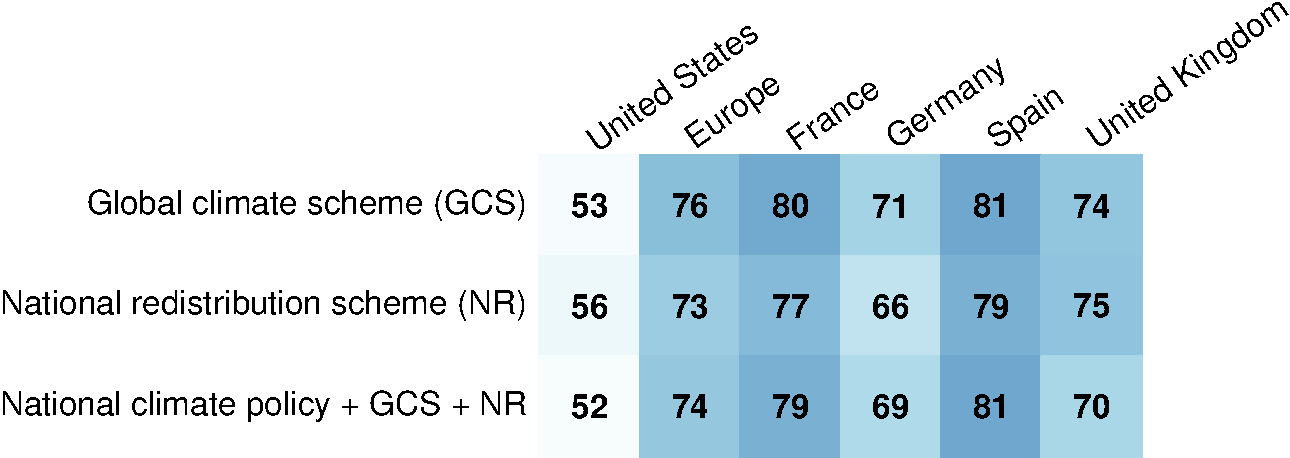
\includegraphics[width=.9\textwidth]{../figures/country_comparison/support_binary_positive.pdf}} 
% \end{figure}

% TODO?: add note to the figure above, to explain what is the national climate policy.
 
[ED\_Fig1] \refstepcounter{figure}\label{fig:ca_r}
% \begin{figure}[h] 
%   \caption[Preferences for various policies in political platforms]{Effects of the presence of a policy (rather than none from this domain) in a random platform on the likelihood that it is preferred to another random platform. (See non-translated versions in Figure \ref{fig:ca_r_en}; Question \ref{q:conjoint_r}%; in the U.S., asked only to non-Republicans.
%   )}\label{fig:ca_r}
%   \begin{subfigure}{\textwidth}
%     \subcaption{U.S. (Asked only to non-Republicans)}
%     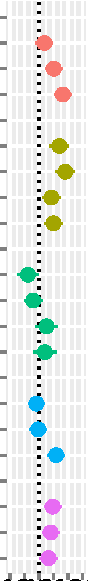
\includegraphics[width=\textwidth]{../figures/US1/ca_r.pdf}
%   \end{subfigure}
%   \begin{subfigure}{\textwidth}
%     \subcaption{France}
%     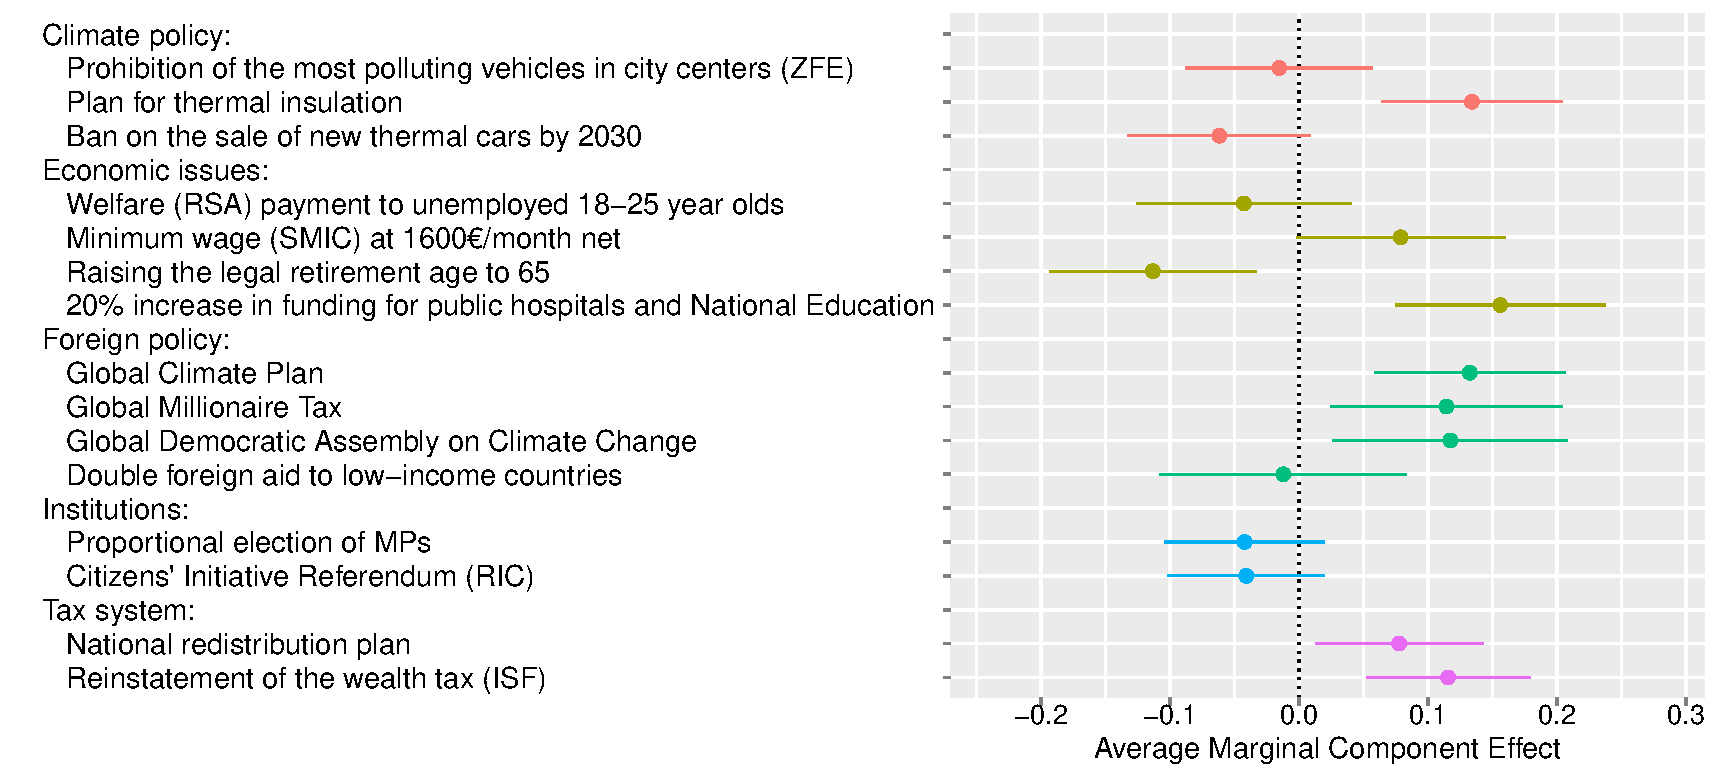
\includegraphics[width=\textwidth]{../figures/FR/ca_r_en.pdf}
%   \end{subfigure}
% \end{figure}%
% \clearpage
% \begin{figure}[h!]\ContinuedFloat % if bugs try b! instead of h!
%   \begin{subfigure}{\textwidth}
%     \subcaption{Germany}
%     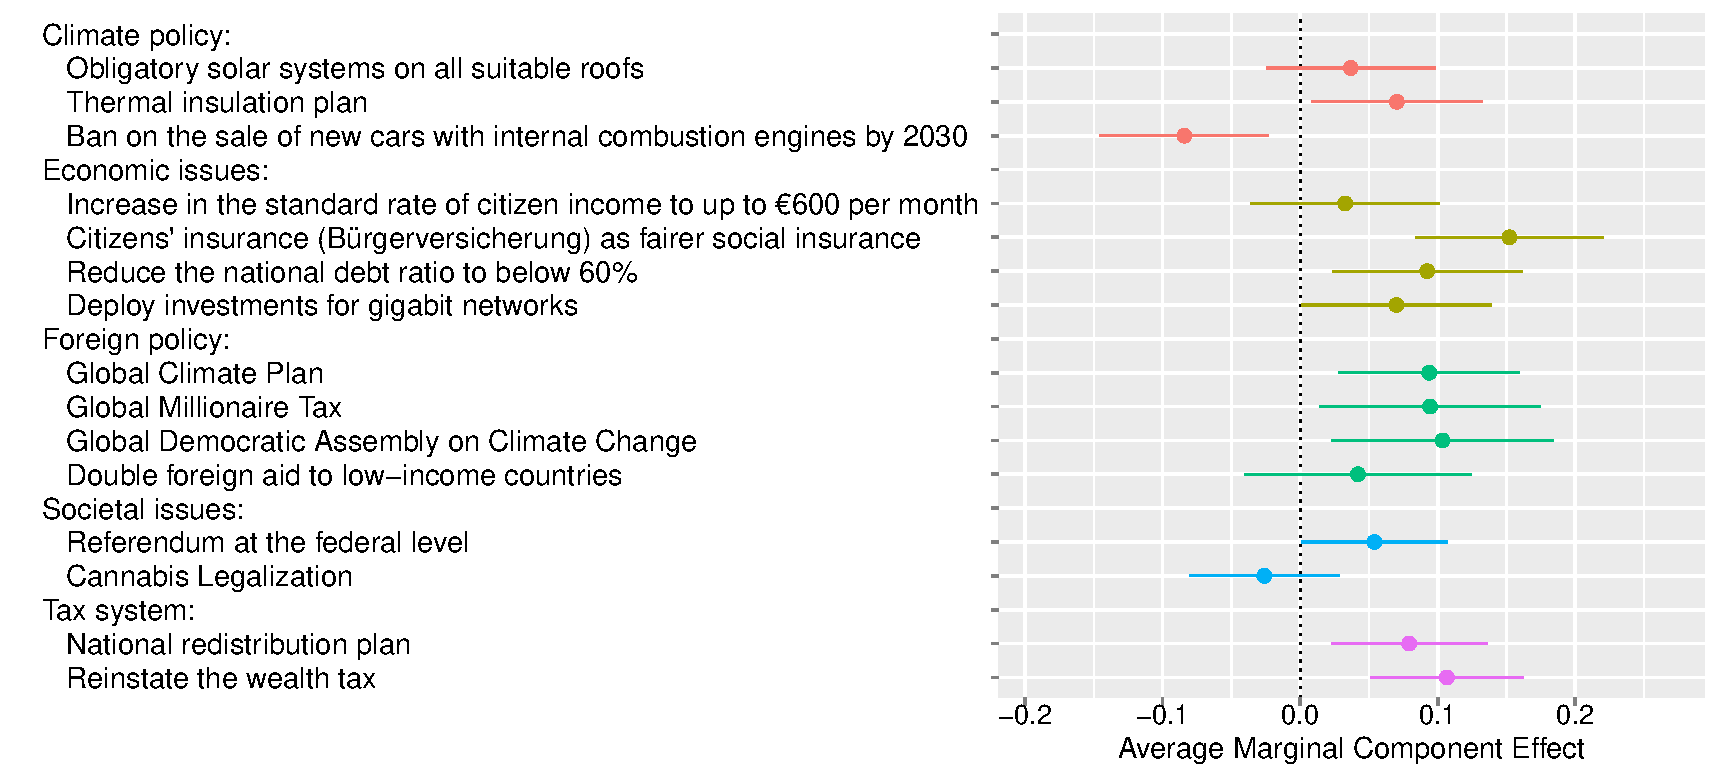
\includegraphics[width=\textwidth]{../figures/DE/ca_r_en.pdf}
%   \end{subfigure}
%   \begin{subfigure}{\textwidth}
%     \subcaption{Spain}
%     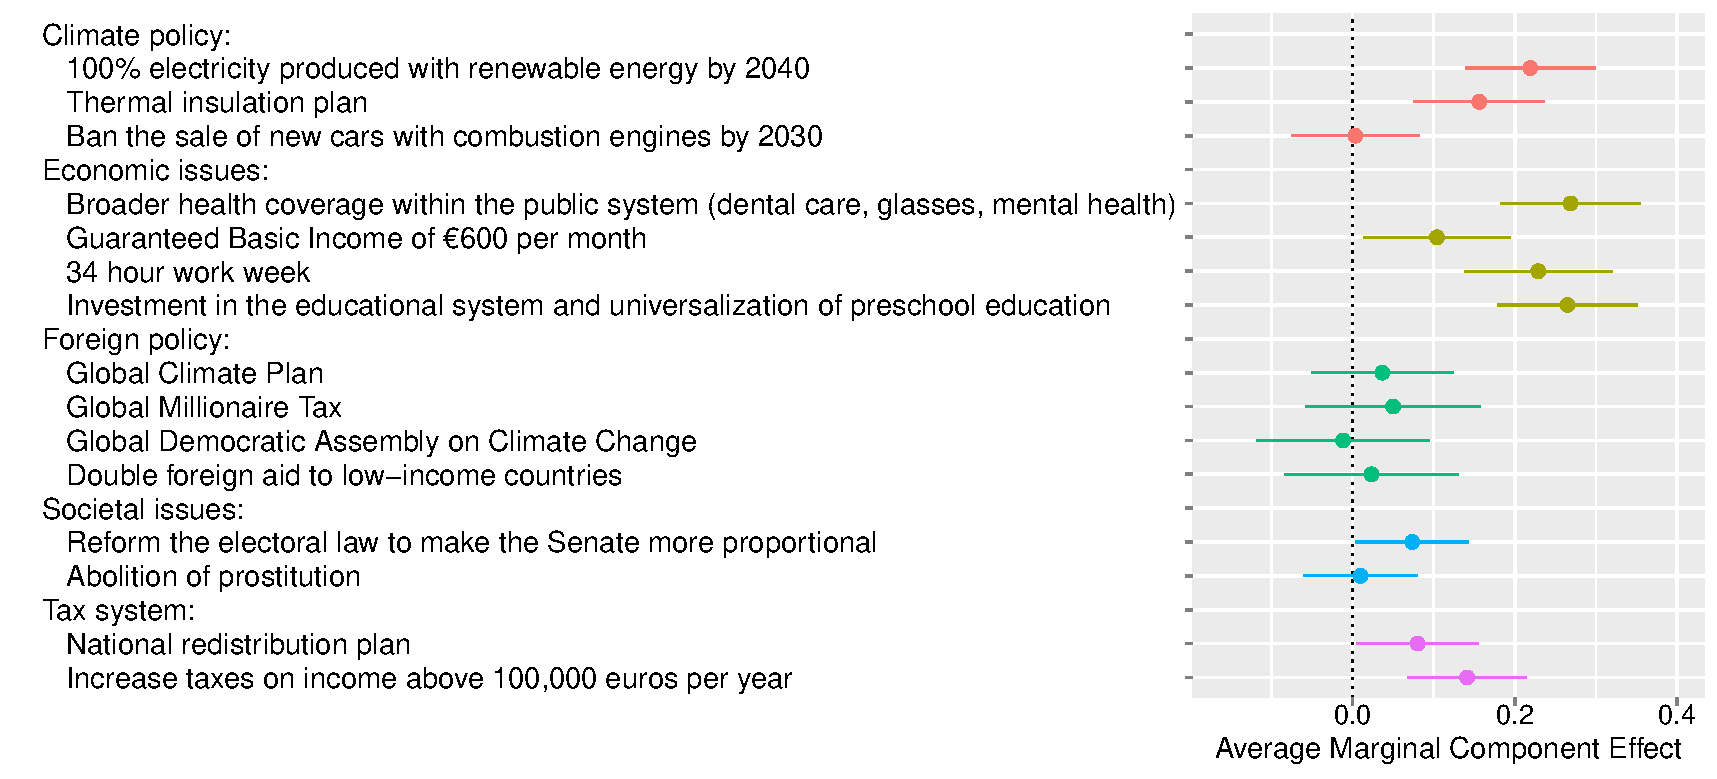
\includegraphics[width=\textwidth]{../figures/ES/ca_r_en.pdf}
%   \end{subfigure}
%   \begin{subfigure}{\textwidth}
%     \subcaption{UK}
%     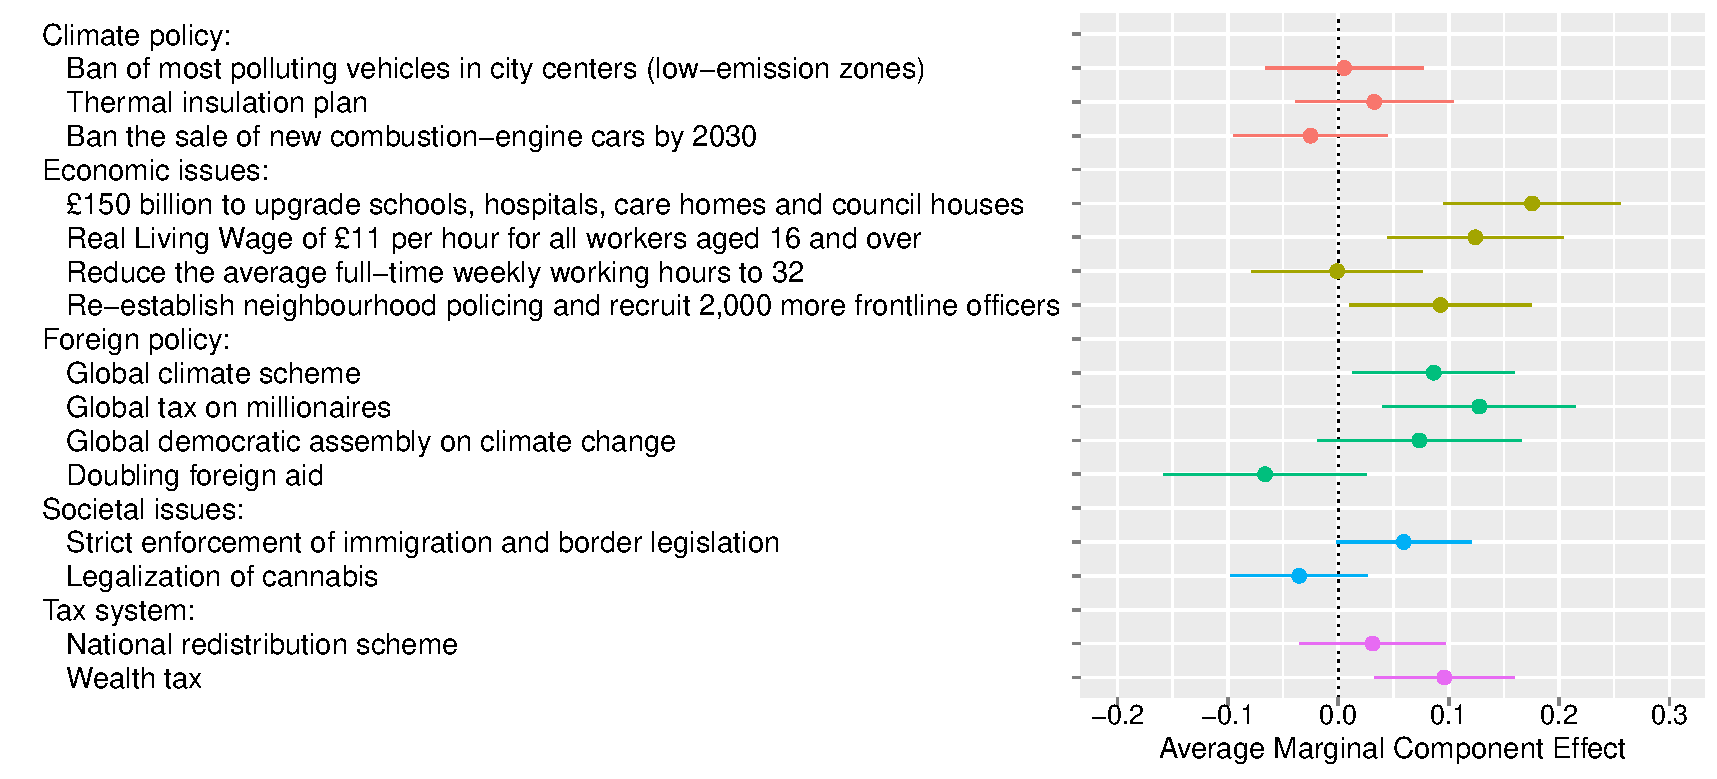
\includegraphics[width=\textwidth]{../figures/UK/ca_r.pdf}
%   \end{subfigure}
%   %\makebox[\textwidth][c]{} 
% \end{figure}

[ED\_Fig2] \refstepcounter{figure}\label{fig:conjoint_left_ag_b}
% \begin{figure}[h!]
%   \caption[Influence of the GCS on preferred platform]{Influence of the GCS on preferred platform:\\ Preference for a random platform A that contains the Global Climate Scheme rather than a platform B that does not (in percent). (Question \ref{q:conjoint_d}; in the U.S., asked only to non-Republicans.)}\label{fig:conjoint_left_ag_b}
%   \makebox[\textwidth][c]{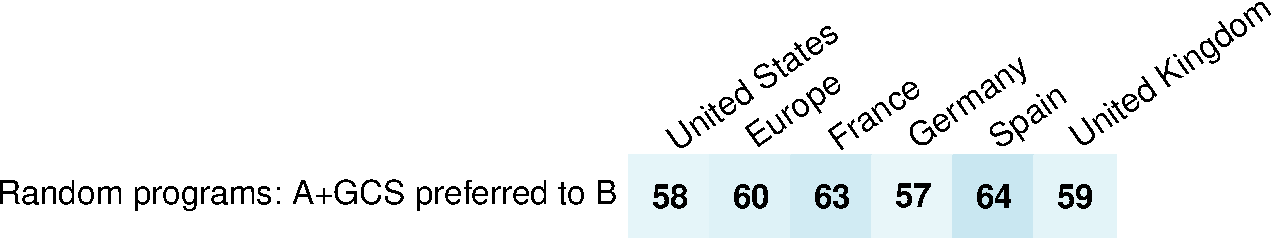
\includegraphics[width=\textwidth]{../figures/country_comparison/conjoint_left_ag_b_binary_positive.pdf}} 
% \end{figure}

[ED\_Fig3] \refstepcounter{figure}\label{fig:belief}
% \begin{figure}[h!]
%   \caption[Beliefs about support for the GCS and NR]{Beliefs regarding the support for the GCS and NR. (Questions \ref{q:gcs_belief} and \ref{q:nr_belief})}\label{fig:belief}
%   \makebox[\textwidth][c]{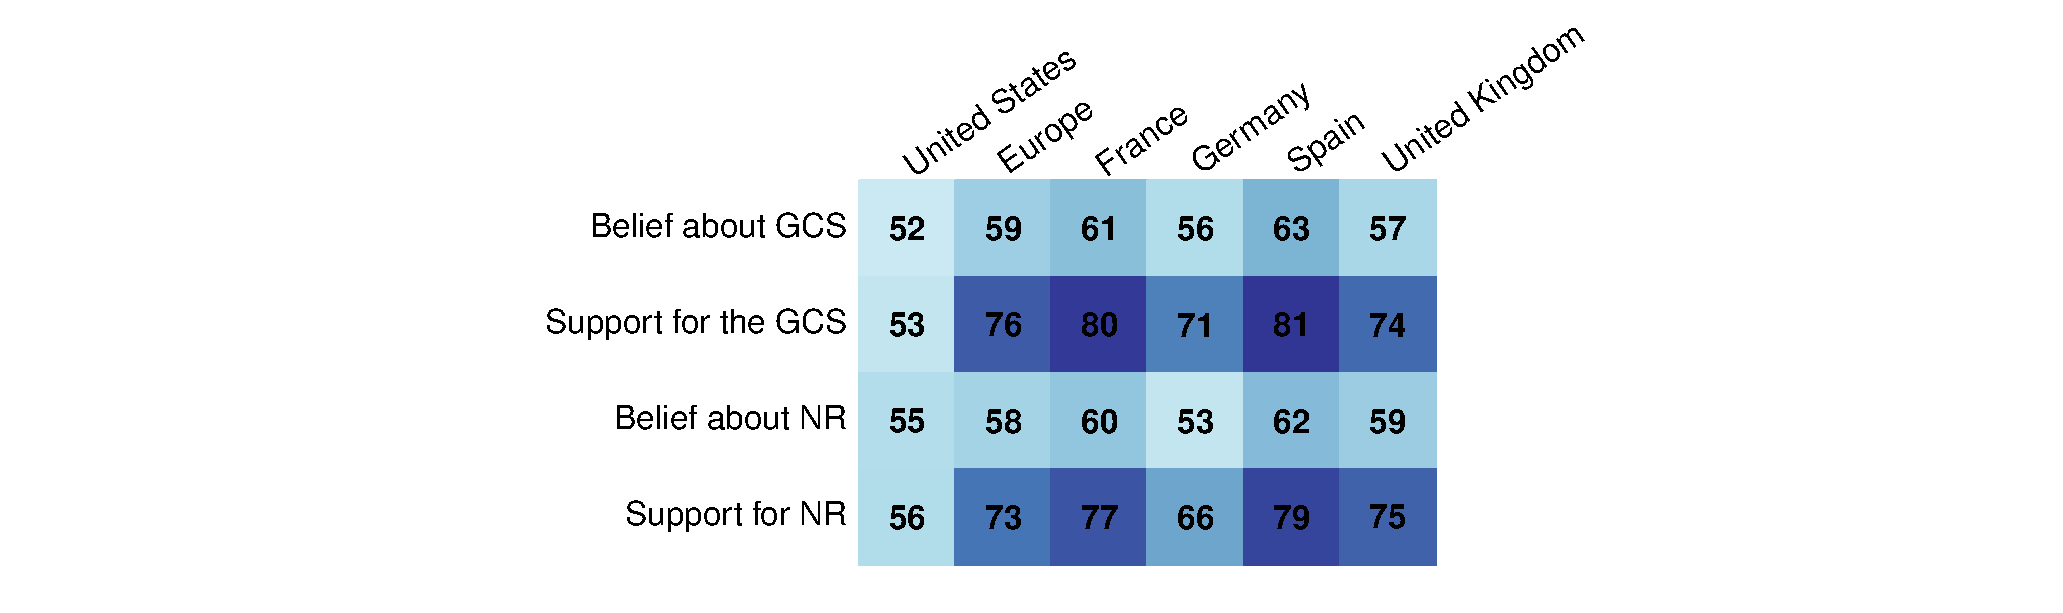
\includegraphics[width=.7\textwidth]{../figures/country_comparison/belief_all_mean.pdf}} 
% \end{figure}

[ED\_Fig4] \refstepcounter{figure}\label{fig:global_share_mean}
% \begin{figure}
%   \centering 
%   \caption[Preferred share of wealth tax for low-income countries]{Percent of global wealth tax that should finance low-income countries (\textit{mean}). \\ ``Imagine a wealth tax on households with net worth above [\$]5 million, enacted in all countries around the world.  
%   (\dots)  \\
%   What percentage should be pooled to finance low-income countries (instead of retained in the country's national budget)?'' (Question \ref{q:global_tax_global_share})} % TODO? n
%   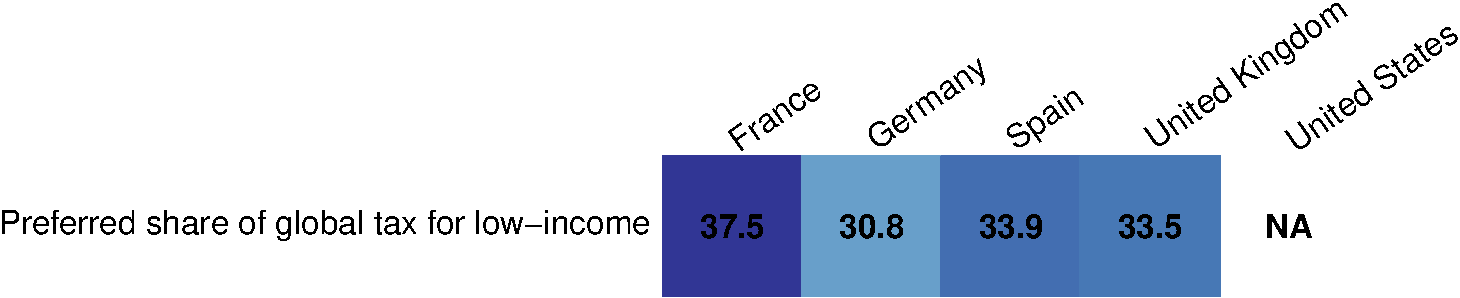
\includegraphics[width=1\textwidth]{../figures/country_comparison/global_tax_global_share_mean.pdf} \label{fig:global_share_mean}
% \end{figure}

[ED\_Fig5] \refstepcounter{figure}\label{fig:foreign_aid_raise_support}
% \begin{figure}[h!]
%   \caption[Attitudes on the evolution of foreign aid]{Attitudes regarding the evolution of [own country] foreign aid. (Question \ref{q:foreign_aid_raise_support})}\label{fig:foreign_aid_raise_support}
%   \makebox[\textwidth][c]{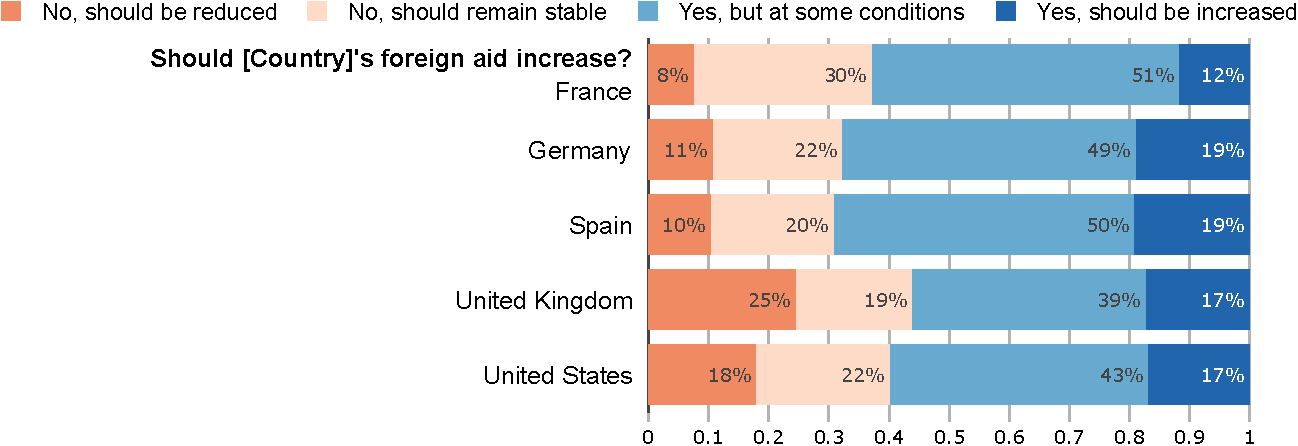
\includegraphics[width=\textwidth]{../figures/country_comparison/foreign_aid_raise_support.pdf}} 
% \end{figure}

[ED\_Fig6] \refstepcounter{figure}\label{fig:foreign_aid_condition}
% \begin{figure}[h!]
%   \caption[Conditions at which foreign aid should be increased]{Conditions at which foreign aid should be increased (in percent). [Asked to those who wish an increase of foreign aid at some conditions.] (Question \ref{q:foreign_aid_condition})}\label{fig:foreign_aid_condition}
%   \makebox[\textwidth][c]{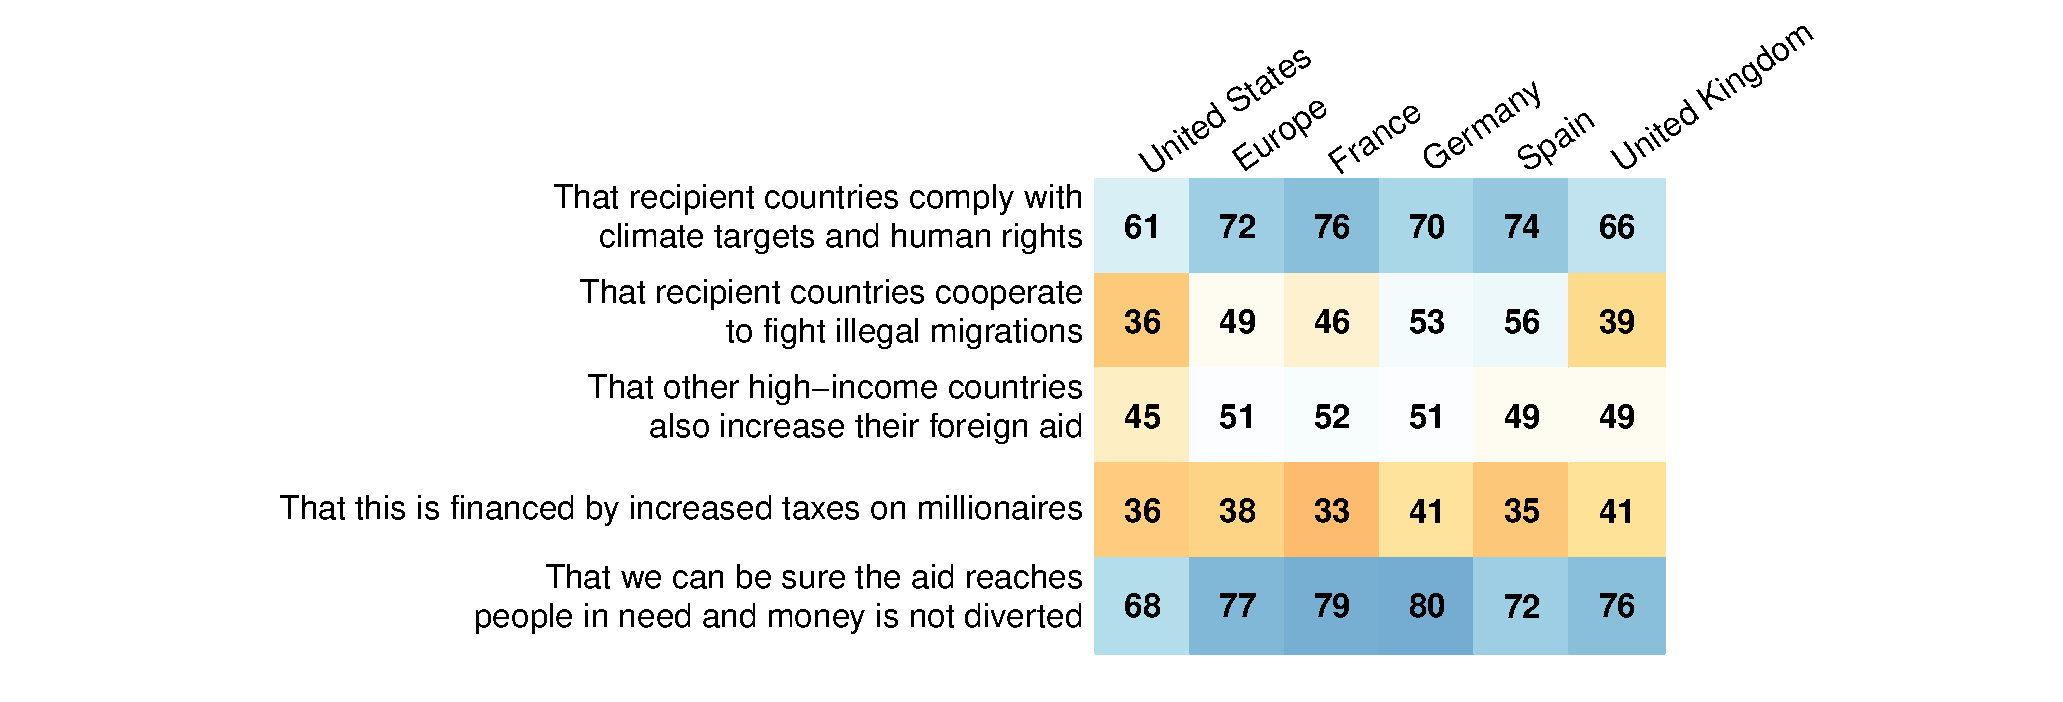
\includegraphics[width=\textwidth]{../figures/country_comparison/foreign_aid_condition_positive.pdf}} 
% \end{figure}

[ED\_Fig7] \refstepcounter{figure}\label{fig:foreign_aid_no}
% \begin{figure}[h!]
%   \caption[Reasons why foreign aid should not be increased]{Reasons why foreign aid should not be increased (in percent). [Asked to those who wish a decrease or stability of foreign aid.] (Question \ref{q:foreign_aid_no})}\label{fig:foreign_aid_no}
%   \makebox[\textwidth][c]{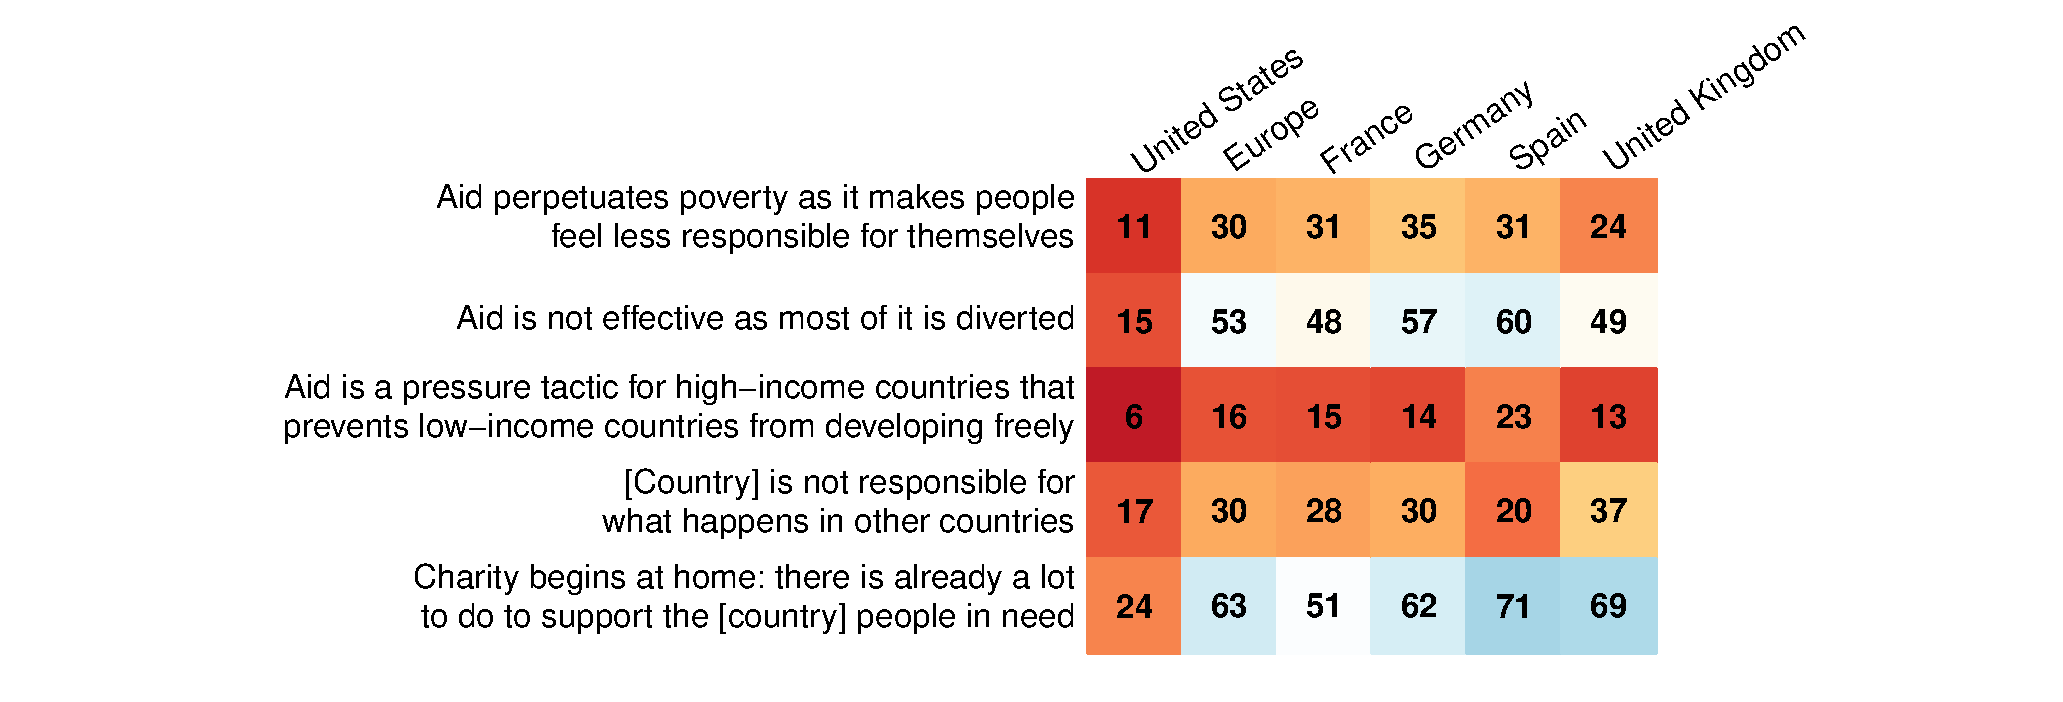
\includegraphics[width=\textwidth]{../figures/country_comparison/foreign_aid_no_positive.pdf}} 
% \end{figure}

% \renewcommand{\thetable}{S\arabic{table}}
% \renewcommand{\thefigure}{S\arabic{figure}}
% \setcounter{figure}{0}
% \setcounter{table}{0}

% % TODO! list experiment, world citizenship, elite surveys, etc.
% TODO Norway and foreign aid
\clearpage
\section{Literature review}\label{sec:literature}

\subsection{Attitudes and perceptions}\label{subsec:literature_attitudes}

\subsubsection{Population attitudes on global policies}\label{subsubsec:literature_attitudes_policies}
% Our surveys fill gaps in the knowledge of attitudes toward global policies. 
% We are not aware of any other survey on a global wealth tax. 
\citet{carattini_how_2019} test the support for different variants of a global carbon tax, but their samples are representative only along gender and age, and as respondents face only one variant, the sample size for a given variant is about 167 respondents per country. They find more than 80\% of support for any variant in India, between 50 and 65\% in Australia, the UK and South Africa, and 43 to 59\% of support in the U.S., depending on the variant. The support for a global carbon tax funding an equal dividend for each human is close to 50\% in high-income countries (e.g. at 44\% in the U.S.), consistently with what we find in the global survey (see Figure \ref{fig:oecd}). This is another piece of evidence that the support is lower for a tax that would ``only'' reduce CO$_\text{2}$ emissions than for a quota that would unambiguously achieve the climate target. %Given that \citet{carattini_how_2019} do not explain that the policy would reduce extreme poverty and test a \textit{tax} that would only reduce CO$_\text{2}$ emissions (rather than achieve the climate target), the support is consistent with the support for a tax observed in the global survey (see Figure \ref{fig:oecd}), and somewhat lower than what the support for the GCS. 
Using a conjoint analysis in the U.S. and Germany, \citet{beiser-mcgrath_could_2019} find that the support for a carbon tax increases by up to 50\% % e.g. in their Fig. 4 the DE support for $70/t jumps from 26 to 39% with extension to all industrialized countries
if it applies to all industralized countries rather than just one's own country. % Variant of carbon tax is 8 (US) - 17 (DE) p.p. more likely to be preferred if tax is extended to all industrialized countries

In surveys in Brazil, Germany, Japan, the UK and the U.S., \citet{ghassim_who_2020} finds 55 to 74\% of support for ``a global democracy including both a global government and a global parliament, directly elected by the world population, to recommend and implement policies on global issues''. % (for example, international peace, world poverty, and climate change)''
Using an experiment, he also finds that, in countries where the government stems from a coalition, voting shares would shift by 8 (Brazil) to 12 p.p. (Germany) from parties who are said to oppose global democracy to parties that supposedly support it. For example, the Greens and the Left gained respectively 9 and 3 p.p. in vote intentions while the SPD and the CDU-CSU each lost 6 p.p., when Germans respondents were told that (only) the former parties support global democracy. 
\citet{ghassim_who_2020} also document survey results which show strong majorities support in each of 18 countries for the direct election of one's country's UN representative. % same as unpa_survey_2005 % GlobeScan 2005; also: half/half (majorities or not depend on the country) for “Global Parliament, where votes are based on country population sizes, and the global parliament is able to make binding policies” (Synovate 2007); also: (GlobeScan 22, not from Ghassim) in 31 countries: 77% agree that “Rich countries must pay for poorer countries do deal with the effects of CC” 
Similarly, in each of 10 countries, there are clear majorities in favor of ``a new supranational entity [taking] enforceable global decisions in order to solve global risks'' \citep{global_challenges_foundation_attitudes_2018}. Actually, already in 1946, 54\% of Americans agreed (and 24\% disagreed) that ``the UN should be strengthened to make it a world government with the power to control the armed forces of all nations'' \citep{gallup_seventy_1946}. 
In surveys in Argentina, China, India, Russia, Spain, and the U.S., \citet{ghassim_public_2022} find support for UN reform that would make United Nations' decisions binding, give veto powers at the Security Council to a few other major countries, and complement the highest body of the UN with a chamber of directly elected representatives. 

Relatedly, \citet{meilland_international_2023} find that Americans and French people prefer an international settlement of climate justice even if it empedes on sovereignty. In a 2013 survey in China, Germany and the U.S., \citet{schleich_citizens_2016} show that more than three quarter of people think that international climate agreements reached so far are not successful and that future agreements are important. % 73\% of people find important future international climate agreements, while less than 26\% think that international reached so far are successful. 
In Finland, \citet{sivonen_attitudes_2022} finds that a carbon tax receives higher support if enacted at the global level (54\%) rather than at the national level (40\%).

These specific questions are in line with the answers to more general questions. In each of 36 countries, \citet{issp_international_2010} find near consensus that ``for environmental problems, there should be international agreements that [their country] and other countries should be made to follow'' (overall, 82\% agree and 4\% disagree). % No question like this in the next Envi wave in 2022
In each of 29 countries, \citet{issp_international_2019} uncover near consensus that ``Present economic differences between rich and poor countries are too large'' (overall, 78\% agree and 5\% disagree). 
%* Also in ISSP (19): slight minorities (in rich countries) that “People in wealthy countries should make an additional tax contribution to help people in poor countries.” p. 104, but strong majorities everywhere that “People from poor countries should be allowed to work in wealthy countries.” p. 106

%* ISSP (19): Near consensus that “Present economic differences between rich and poor countries are too large.” p. 102, slight minorities (in rich countries) that “People in wealthy countries should make an additional tax contribution to help people in poor countries.” p. 104, but strong majorities everywhere that “People from poor countries should be allowed to work in wealthy countries.” p. 106
%* Ghassim et al. (22): support for stronger UN with more direct elections.
%* Ghassim (20):  in Germany those two parties that supposedly endorse global democracy – the Greens and the Left – benefitted, gaining nine and three percentage points respectively in terms of voting intentions. Meanwhile, the traditional centrist parties – SPD and CDU – each lost six percentage points due to their supposed opposition to global democracy.
%* Beiser-McGrath & Bernauer (19): Conjoint analysis in US, DE. Variant of carbon tax is 8 (US) - 17 (DE) p.p. more likely to be preferred and 50% more likely to be supported if tax is extended to all industrialized countries (Fig 1, 4). (Unfortunately, don't test extension to global level).
%- Çarkoğlu.. (15) International Social Survey Program 2010 data reveal that people in LDCs are less supportive of international agreements forcing their country to take necessary environmental measures than are citizens in the developed world [80% instead of 85%]. (‘for environmental problems, there should be international agreements that [their country] and other countries should be made to follow.’)
%* Carattini et al. (Nature, 19): 1k in US, IA, ZA, AU, UK. Each respondent receives one variant at random of global carbon price of 40/60/80 $/t redistributed as international dividend / national dividend / mitigation in all countries / mitigation in developing countries / domestic mitigation / reduced labour tax. Immense majorities for any scheme in India, small majorities for each elsewhere except US international dividend (44%) or mitigation in developing (43%), and AU mitigation in developing (49,6%). PB: very low sample size (~167) for a given redistribution, even lower (~55) for a given variant (that also specifies the price). Appendix also contains estimation of distributive impacts. Representative only along the two quotas: gender and age. Don't give the representativeness in terms of income (the third socio-demos that they ask) so it's probably bad.

\subsubsection{Population attitudes on climate burden sharing}\label{subsubsec:literature_attitudes_burden_sharing}

Despite their differences in the description of the fairness principles, the surveys on burden-sharing rules show consistent attitudes. Or at least, their various results can be made compatible with the following interpretation: 
Concerning emissions reductions, most people want that every country engage in strong decarbonization effort together, with a global quota converging to climate neutrality in the medium run. Concerning the financial effort, most people support high-emitting countries paying and low-income countries receiving funding. The most supported rules are those that appear equitable, in particular an equal right to emit per person. 
% When the rankings between rules differ, it can be due to the difference in countries surveyed, but it is most often due to differences in definitions and wording. 

This interpretation helps understanding the apparent differences between articles, which approach burden sharing from different angles: cost sharing (i.e. in money terms), effort sharing (in terms of emissions reductions), or resource sharing (in terms of rights to emit). Extant papers adopt the cost sharing or effort sharing approaches and preclude any country being a net receiver of money. Also, by focusing on \textit{either} the financial or the decarbonization effort, these surveys miss the other half of the picture, which can explain why some papers find strong support for the ability-to-pay principle while others find strong support for grandfathering (defined as emissions reductions being the same in every country). The literature follows these approaches to stick to the terms used by the UNFCCC. Yet, we argue that the resource sharing approach is preferable to uncover attitudes, as it unambiguously describes the distributive implications of each rule while achieving an efficient location of emissions reductions and explicitly allowing for monetary gains for some countries. % TODO? say more simply that the location of emissions reductions is flexible in resource sharing
% TODO? appendix with the definitions for each author, incl. us

Now, let us summarize the different papers' results in the light of this clarification. 
\citet{schleich_citizens_2016} find an identical ranking in the support for the burden-sharing principles in China, Germany, and the U.S.: polluter-pays followed by ability-to-pay, equal emissions per capita, and grandfathering. 
% \footnote{The survey of \citet{schleich_citizens_2016} defines these rules as follows: \\
% \textit{Polluter-pays}: ``Every country has to bear costs according to the emissions it causes (hence countries causing higher emissions have a higher share of the costs).'' \\
% \textit{Ability-to-pay}: ``Every country has to bear costs according to its economic strength (hence richer countries have a higher share of the costs).''
% \textit{Egalitarianism}: ``Every country is allowed to produce the same amount of emissions per capita (hence countries with currently high emissions per capita have higher costs).''
% \textit{Sovereignty} (i.e. grandfathering): ``Every country is allowed to produce the same share of global emissions as in the past (hence the proportional reduction of emissions is the same for every country).''} 
Note that the authors do not allow for emissions trading in their description of equal \textit{emissions per capita}, which may explain its relatively low support. 
Yet, the relative support for egalitarianism also depends on how \textit{the other} rules are described. Indeed, \citet{carlsson_is_2011} find that Swedes prefer that ``all countries are allowed to emit an equal amount per capita'' rather than options where emissions are reduced in relation to current or historical emissions for which it is explicitly written that high-emitting countries ``will continue to emit more than others''. 
\citet{bechtel_mass_2013} find agreement that rich countries should pay more and historical emissions matter, but that rich countries should not be the only ones to make the efforts. More precisely, their conjoint analysis in France, Germany, the UK and the U.S. shows that a climate agreement is 15 p.p. more likely to be preferred  (to a random alternative) if it includes 160 countries rather than 20, and 5 p.p. less likely to be preferred if ``only rich countries pay'' compared to other burden-sharing rules: ``rich countries pay more than poor'', ``countries pay proportional to current emissions'' or ``countries pay proportional to historical emissions''. %=> confirms preference for global policies (rather than only partial coverage). Finds that costs is what matters most: preference decreases by 30pp if it’s 2.5\% of GDP compared to 0.5\%.
% I have sent an email on 3/3/23 to get access to desc stats of Bechtel et al (19)
Using a choice experiment, \citet{carlsson_fair_2013} find that the least preferred option in China and the U.S. is when low-emitting countries are exempted from any effort. Ability-to-pay is appreciated in both countries, though the preferred option in China is another one, which accounts for historical responsibility. %that Americans prefer capacity to pay > current responsibility > historical responsibility > equal emissions per capita while Chinese prefer historical > capacity > current > equal emissions.
%   Capacity to pay: Countries with high income levels must pay a larger share of the costs than countries with low income levels. This option says that countries with greater ability to pay should pay more
%   Current responsibility: Countries with currently high emissions levels must pay a larger share of the costs than countries with currently low emissions levels. This option says that those countries that are currently a larger part of the problem should pay more.
%   Historical responsibility: Countries with a history of high emissions levels must pay a larger share of the costs than countries with a history of lower emissions. This option recognizes that CO2 builds up in the atmosphere over many years. Thus, countries with a history of high emissions should pay more because they caused more of the problem.
%   Equal emissions pc: Countries with emissions per person greater than an agreed amount must pay, and they must pay more the higher their emissions per person are.
% > "equal emissions" is a misnomer as this is about costs (not emissions) and it's just a more progressive version of current responsibility / polluter-pay, where high-emitting pay more and low-emitting don't pay. The result for US is compatible with the other papers as Americans agree that rich countries (or high-emitting, the diff is small) should pay more. The Chinese position could also be reconciliable once we define responsibility from footprint rather than territorial and that there will be transfers from rich to poor countries.
In the U.S. and France, \citet{meilland_international_2023} find that the most favored fairness principle is that ``all countries commit to converge to the same average of total emissions per inhabitant, compatible with a controlled climate change''. Furthermore, in each country, 73\% disagree with grandfathering defined as ``countries which emitted a lot of carbon in the past have a right to continue emitting more than others in the future''. \citet{meilland_international_2023} contain many other results, for example majorities prefer to hold countries accountable for their consumption-based rather than territorial emissions, and the median choice regarding historical responsibility is to hold a country accountable for their post-1990 emissions (rather than post-1850 or just their current emissions). 
% - Meilland et al. (23) find that in US and France, most favored fairness principle is Equality in per capita emissions: "all countries commit to converge to the same average of total emissions per inhabitant, compatible with a controlled climate change" and second-most (which closely follows) is grandfathering: "all countries commit to reduce their emissions by a same proportion". 73% in each disagree with grandfathering when defined as "countries which emitted a lot of carbon in the past have a right to continue emitting more than others in the future". To rationalize these contrasted views with grandfathering, we can interpret them as: equal rights, equal emission reductions, and transfers. 
%   convergence per capita (70%): all countries commit to converge to the same average of total emissions per inhabitant, compatible with a controlled climate change
%   grandfathering (60%): all countries commit to reduce their emissions by a same proportion
%   past emissions (20% choose it among their two favorite): countries which emitted less in the past commit to reduce their emissions less than other countries
%   poor countries (20%): poorer countries commit to reduce their emissions less than richer countries
%   cost-efficiency (20%): countries where reducing emissions is more costly commit to reduce their emissions less than other countries
% - Meilland et al. (23) Other findings: people prefer international settlement on CC even if it empedes on sovereignty, a majority prefers to target footprint rather than territorial emissions, median is that countries should be held accountable for post-1990 emissions, self-serving bias when judging e.g. India vs. EU, no shared understanding of fairness when asked to coordinate between French and Americans
Finally, in each of 28 (among the largest) countries, \citet{dabla-norris_public_2023} find strong majority for ``all countries'' to the question ``Which countries do you think should be paying to reduce carbon emissions?''. Asked to choose between a cost sharing based on \textit{current} vs. \textit{accumulated historic emissions}, a majority prefers \textit{current emissions} in all countries but China and Saudi Arabia (where the two options are close to equally preferred). %In Germany and the U.S., \citet{gampfer_obtaining_2014} also find stronger support for funding climate action in low-income countries when cost is shared with other countries.

%- Gampfer (14): lab experiment (ultimatum game) to test whether preferences respect fairness principles

\subsubsection{Population attitudes on foreign aid}\label{subsubsec:literature_foreign_aid}

There is an extensive literature on attitudes toward foreign aid in donor countries. Its main insights are that most people overestimate the amount of foreign aid and that only a minority wants a cut in foreign aid compared to actual amounts, especially once they know them. 

\citet{pipa_americans_2001} shows that 83\% of Americans support a multilateral effort to cut world hunger in half. 
\citet{pipa_publics_2008} shows that in each of 20 countries, a majority thinks that developed countries ``have a moral responsibility to work to reduce hunger and severe poverty in poor countries'', with an average agreement of 81\%. In 7 OECD countries, they find that at least 75\% are willing to pay for a program to cut hunger in half (at an estimated cost of e.g. \$50 a year for each American). 

\citet{kaufmann_foreign_2012} find that in each of 24 countries, perceived aid is overestimated, on average by a factor 7. In most countries, desired aid is larger than perceived aid.\footnote{\citet{kaufmann_foreign_2012} offer the best results on desired aid because (as \citet{hudson_mile_2012} criticize), other studies did not take into acount misperceptions of actual aid.} They show that those in the top income quintile desire aid 0.13 p.p. lower than those in the bottom 40\% -- which is very close to what we find. % TODO: ref to our regression
Then, using a theoretical model as well as correlations between the level of lobbying and the actual aid (controling for desired aid), they argue that the gap between actual and desired and is due to political influence of the rich who defend their vested interests. 
In \citet{kaufmann_foreign_2012}, the U.S. is an outlier: desired aid is at the other countries' average (3\% of GNI), but as misperceptions are enormous, perceived aid is twice as large as desired aid. Indeed, \citet{gilens_political_2001} shows that even American with high political knowledge misperceive actual aid, and finds that 17\% fewer of them want to cut aid when we provide them specific information about aid amount. % same for Hurst et al
Similarly, \citet{nair_misperceptions_2018} finds that the relatively low support for aid in the U.S. is driven by information on global distribution, as people underestimate their rank by 27 centiles on average and overestimate the global median income by a factor 10. 

\citet{hudson_mile_2012} offer a critical review of the literature and show that the strong support for poverty alleviation largely stems from intrinsic altruism. Indeed, citing \citet{dfid_aid_2009} and \citet{pipa_americans_2001}, they note that 47\% of British people find that the aid is wasted (mainly due to corruption), while Americans estimate that less than a quarter of the aid reaches people who really need it and more than half ends up in the hands of corrupt government officials. And yet, most people still support aid, suggesting that they have nonutilitarian motives for doing so. Consistent with \citet{henson_public_2010}, \citet{bauhr_does_2013} find that support for aid is reduced by perception of corruption in recipient countries. However, this effect is reduced by the aid-corruption paradox: most corrupt countries need more help. \citet{bodenstein_who_2017} further show that right-wing Europeans or those who perceive strong corruption in their country are more likely to agree that recipient countries should ``follow certain rules regarding democracy, human rights and governance as a condition for receiving EU development aid.'' 
Using a 2002 Gallup survey as well as the 2006 World Values Survey, and consistently with \citet{bayram_aiding_2017}, \citet{paxton_individual_2012} show that the main determinants for wanting more aid are trust, left-wing ideology, interest in politics, and being a woman (all positively associated). %Likewise, \citet{nair_preferences_2016} shows that preferences for international redistribution in the U.S. are netter explained by worldviews rather than socio-demographic variables. 
% heinrich_voters_2018 also show that the country's interest also play a role in aid support (as support increases when the donation can be in the country's interest) 

% Reviews, determinants
%*? Milner & Tingley (13): (highly cited but no original data, don't think we need to cite it) In 2008, 44% of American wanted foreign aid cut (american elections study, 08). fraction of federal budget going to foreign aid (mean: 27%, median: 25%) / should go (mean: 13%, median: 10%) (WorldPublicOpinion, 10)
% PIPA (01): when PIPA asked respondents to estimate how much of the federal budget was devoted to foreign aid, the median estimate was 15% -- 15 times the actual amount, which was just under 1%. More dramatically, when asked what an appropriate percentage would be, the median response was 5% -- 5 times the actual amount. And when asked to imagine that they heard the real amount was only 1%, only 18% of respondents said they thought that would be too much--as compared to the 75% who had initially said that the US was spending too much. 
%- DFID (10): Priorities: 1 NHS, 2 education, 3 support to poor countries, 4 police, 5 defence (p. 19). Show majority support for increased aid until 07, then median is to support stable aid (due to crisis?). It seems they don't give the info on actual amount though.
%* Hudson & van Heerde (12):Reviews literature on foreign aid and criticizes it on a number of points (e.g. not uncovering the determinants, and not asking well the questions). Shows strong support for poverty alleviation, (at least partly) out of intrinsic altruism. Use 4 main sources: PIPA (01, 08) UK DIDP, Eurobarometer; cf. Table 1 for all surveys on foreign aid / Public support for development has been famously described as a mile wide and and inch deep (Smillie, 1996: ref impossible to find). Hard times at home have meant that public support appears to have turned against international development efforts (Henson and Lindstrom, 2010). / Monitor public support: (Fransman and Solignac Lacomte, 2004; McDonnell et al, 2003), Paxton and Knack, 2008; Chong & Gradstein 2006. Review surveys on aid. / ~75% support aid in developed countries (stable) but ‘84 per cent agreed with the assertion that ‘taking care of problems at home is more important than giving aid to foreign countries’ (PIPA, 2001:9).” / References on covariates of aid support / PIPA 2001, "On average, Americans thought just under 25 per cent of the US budget was allocated to foreign aid, and government should allocate less than 14 per cent of the national budget. However, when told that US spends approximately 1 per cent of the federal budget on foreign aid, 37 per cent of respondents thought this was too little, 44 per cent thought it was about right, and 13 per cent thought it too much."  Think that only 23% of aid really goes to the poor / “The 2009 UK survey, Public Attitudes towards Development, reports ‘public support for overseas aid’ at 72 per cent (DFID, 2009); while in the US support was a comparable 79 per cent (PIPA, 2001); and average support across the EU trends slightly higher than in the US and UK with 91 per cent saying it was either very (53%) or fairly (38%) important to provide aid to poor countries (Eurobarometer, 2005).” / “DFID has now begun asking questions that provide relative measures of the salience of development aid vis-à-vis other competing policy issues (DFID, 2009; IDC, 2009). / "high proportion (61%) of US citizens who felt that the US spends too much on foreign aid. [from another source]” / “The distinction between foreign aid, which includes military spending, and development aid/assistance is an important one” / “81 per cent of respondents believed that developed countries do have a moral responsibility to work towards reducing hunger and severe poverty (WorldPublicOpinion.org, 2008). (…)  %/ “support for development assistance is highly contingent on respondents’ perceptions of the effectiveness of aid, especially with regard to corruption (Henson et al, 2010). For example, 
%(…) international charities and NGOs are deemed best suited/most effective compared to donor countries” / UK ‘MyAid’ plan – where the public gets to vote on how a pot of money should be distributed – / "public engagement should be about ‘opening up the political and wider societal space to the possibility of deeper change’ (Darnton and Kirk, 2011:14).”
%- Chong & Gradstein (16): from WVS 95-99, 58% want that their country give more foreign aid (but misperceptions are not taken into account)
%- Williamson (19): Public Ignorance or Elitist Jargon? Reconsidering Americans’ Overestimates of Government Waste and Foreign Aid. "Foreign aid" encompasses military spending, in the mind of American.
%- McDonnell et al (03) Public Opinion and the Fight against Poverty
%- Nair (16): preferences driven by worldviews rather than self-interest
%- Scotto et al (17): We Spend How Much? Misperceptions, Innumeracy, and Support for the Foreign Aid in the United States and Great Britain. Less American and British want aid cut when information on current aid is given in % of GDP rather than in $.
%* Paxton & Knack (12): Majorities want more aid, and main determinants are trust, ideology, interest in politics, and female (all positive). Gallup 02: in US 45% want more aid (rather than stable) vs. 68-91 in DE-UK-ES. Like Chong & Gradstein, find that desired aid increases with income, contrary to Kaufmann et al. but the latter contains more datasets.
%- Wood (15): Determinants for aid support in Australia. Wood (18) Examine Australian support for aid: although there is support to help foreign poor, people back recent aid cuts.
%- Cheng & Smyth (16): Why Give it Away When You Need it Yourself? Understanding Public Support for Foreign Aid in China. Political ideology and patriotism main explaining variables for aid support. People in poorer provinces less supportive.
%- Milner & Tingley (10) theory + empirics: who supports aid and why. owners of capital in donor countries tend to gain from aid and thus are more likely to support giving aid
%- Easterly (JEP, 03) Can Foreign Aid Buy Growth? No (disproves Hansen & Tarp).
%- Hansen & Tarp (01) Aid increases growth (empirical evidence)
%- Tresch et al. (22): 66% of Swiss people want to increase their foreign aid; also Borofsky
%- Harris (17): majority of French want to decrease foreign aid when face with a trade-off with other public spending

\subsubsection{Population attitudes on rich tax}\label{subsubsec:literature_wealth_tax}

We are not aware of any previous survey on a global wealth tax,\footnote{We did not find any using the combination of ``survey'' or ``attitudes'' with ``wealth tax'' or ``global wealth tax'' in Google Scholar.} though surveys consistently show strong level of support from national wealth taxes. 
In a comprehensive survey in the UK, \citet{rowlingson_public_2021} show that a wealth tax is the preferred option to raise revenues, that only 8\% state that total net wealth should not be taxed (with little differences between Labour and Conservative voters), and find that the preferred design would be a 1\% or 3\% tax on net wealth above £1 million. 
By asking how much taxes per year should a person with a certain income and wealth level pay, \citet{fisman_americans_2017} finds that the average Americans favors a 0.8\% linear tax rate on unspecified wealth until \$2 million (the highest wealth level tested), and a 3\% linear rate on inherited wealth. %This is consistent with the findings of \citet{chirvi_preferences_2020}. 
Through a conjoint analysis in three high-income countries, \citet{schechtl_tax_2023} find widespread support for a wealth tax (from 78\% in the U.S. to 86\% in Germany and the UK), with a preference for an exemption threshold at \$/\euro{}1 million (rather than 500,000 or 2 million) and little influence of the tax rate or tax unit on the preferred design. 
In 21 OECD countries, the \citet{oecd_main_2019} uncovers strong majority support for higher taxes on the rich to support the poor (with nearly 70\% overall agreement and less than 20\% disagreement). \citet{isbell_footing_2022} finds similarly high level of support in 34 African countries. 
In the UK, \citet{patriotic_millionaires_patriotic_2022} find 69\% support (and 7\% opposition) for a 1.1\% tax on wealth in excess of £10 million. 
In the U.S., \citet{americans_for_tax_fairness_support_2021} find 67 to 71\% support to ``raise taxes for those earning more than \$400,000 a year'', ``raise the income tax rate for those earning over \$1 million a year by 10 percentage points'', or ``apply a 2\% tax on an individual's wealth above \$50 million each year, and 3\% on wealth above \$1 billion''.
%- Gallup (22), US
%- Fight Inequality Alliance India (22), IA

% PIPA (01): what percentage of their "tax dollars that go to help poor people at home and abroad...should go to help poor people in other countries." The mean response was 16% (down a bit from 22% in response to this question in a 1996 PIPA poll). Strikingly, this turns out to be a far higher percentage than is currently given. In 1999, a bit less than 4% of the total spent on the poor went to the poor abroad. Sixty percent of respondents proposed a percentage that was higher than 4%.

% TODO! list experiment

\subsubsection{Population attitudes on ethical norms}\label{subsubsec:literature_wealth_tax}
% \paragraph{World citizenship}

\paragraph{Universalism}
% No need to cite: Buntaine & Prather (18), Diederich & Goeschl (18) Willingness to act for domestic vs. international climate action
Different papers assess belonging to a global identity (see %e.g. \citet{mcfarland_all_2012}, or 
\citet{reysen_psychology_2018} for a review). In the 2005-2008 wave of the World Values Survey, \citet{bayram_what_2015} notes that ``78\% of the participants in 57 countries see themselves as citizens of the world'', though the \href{https://www.worldvaluessurvey.org/WVSDocumentationWV7.jsp}{2017-2022 wave} reveals that more people feel close to their town, region or country than to the world. 
\citet{enke_moral_2023-1} measure universalism, by asking American respondents to split \$100 between a random stranger and a random person with the same income but closer to them. They distinguish different facets of universalism, and define \textit{foreign universalism} as giving to a foreigner rather than a fellow citizen. They find a home bias for most people, which may partly be due to concerns for inequality, as the split involves two persons with the same income, with the foreigner most certainly living in a poorer country than the American and thus enjoying a higher social status. 
That being said, a home bias probably remains once removing the concern for inequality, as 84\% of Americans agree that ``taking care of problems at home is more important than giving aid to foreign countries'' \citep{pipa_americans_2001}. 
\citet{enke_moral_2023} measure universalism and analyze its correlates in 7 countries, and \citet{cappelen_universalism_2022} deploy this method in 60 countries. 
In a lab experiment with students in the U.S., \citet{cherry_accepting_2017} show that a substantial share of people prefer policies detrimental to them due to their egalitarian worldview. 
% Evidence that people are altruistic: they experience higher temperature when they learn they are doing good (Taufik et al. 15), they are sensitive to self-transcending more than self-interested reasons (Evans et al. 13), 

\paragraph{Free-riding}

Although researchers have long explained the lack of climate action by free-riding, surveys consistently show that people support climate mitigation in their country even if other countries defect. \citet{bernauer_how_2015} show this for Americans and Indians, who both overestimate their country's emissions at one third of global total. \citet{beiser-mcgrath_commitment_2019} show this in the U.S. and China using an experimental design. \citet{mcevoy_prospects_2016} show that Americans mostly invoke leadership and morality to justify unliteral climate action. Using a range of methods, \citet{aklin_prisoners_2020} show that the empirical evidence for free-riding is not compelling, and that climate inaction can be equally well explained by distributive conflicts. Finally, through a review of the literature, \citet{mcgrath_how_2017} show that climate attitudes are largely nonreciprocal, and primarily driven by values and perceptions of the policies, rather than by considerations of what other countries do.

\subsubsection{Second-order beliefs}\label{subsubsec:literature_beliefs}

\citet{allport_social_1924} introduced the concept of pluralistic ignorance: a shared misperception concerning others' beliefs. The concept became notorious when \citet{ogorman_pluralistic_1975} showed that, towards the end of the civil rights movement, 47\% of Americans believed that most white people favored segregation while only 18\% actually did so. %\citet{miller_pluralistic_1987} shows that pluralistic ignorance emerges because individuals believe that fear of embarrassment is a sufficient cause for their own behavior but not for the behavior of others. 
\citet{pipa_americans_2001} has shown that 75\% of Americans are willing to pay \$50 a year to cut world hunger in half (the cost of the program), but only 32\% think that the majority would be willing to pay.
\citet{andre_fighting_2021} have documented pluralistic ignorance of climate-friendly norms in the U.S. Similarly, \citet{sparkman_americans_2022} show that Americans underestimate the support for climate policies by nearly half, while \citet{drews_biased_2022} document pluralistic ignorance of carbon tax support in Spain. 
\citet{geiger_climate_2016} show that pluralistic ignorance about concern for climate change leads people to talk less about it as many self-silence themselves. 
% TODO READ Mildenberg & Tingley (19) and improve summary
%- Bursztyn & Yang (21): Review of the field. Misperceptions about others are widespread, asymmetric, much larger when about out-group members, and positively associated with one’s own attitudes.
%* Andre et al. (21): Respondents vastly underestimate the prevalence of climate- friendly behaviors and norms among their fellow citizens. Providing respondents with correct information causally raises individual willingness to fight climate change as well as individual support for climate policies. The effects are strongest for individuals who are skeptical about the existence and threat of global warming.
%- Di Tella et al. (AER, 15): The results of the lab experiment favor the hypothesis that people avoid altruistic actions by distorting beliefs about others' altruism
%- Allport (1924): first book on pluralistic ignorance
%- Allport (40): function of poll is to correct pluralistic ignorance
%- Studies on pluralistic ignorance: business (Buckley et al. 00), against affirmative action (Van Boven 00), political correctness (Braghieri, AER 21), alcohol (Suls & Green, 03), white support for racial segregation (O'Gorman 75), CC (Geiger & Swim 16), hooking up (Lambert et al 03, cf. note for paragraph of pluralistic ignorance), women working outside home in Saudi Arabia (Bursztyn et al. 20)

% \subsubsection{Elite attitudes}\label{subsubsec:literature_beliefs} % TODO!

% \citet{mildenberger_beliefs_2019} survey elites (Congress staffers and international relations scholars) as well as the population in U.S. and China. They document pluralistic ignorance of pro-climate attitudes, egocentric bias, and increasing support after beliefs are updated. 
% \citet{lange_importance_2007} \citet{lange_self-interested_2010}
% \citet{dannenberg_equity_2010}
% \citet{kesternich_negotiating_2021} 
% \citet{hjerpe_common_2011}

% Elite surveys 
%* Mildenberg & Tingley (19): Congress staffers, cf. second-order beliefs
%- Hertel-Fernandez et al. (2019): Survey on US Congress staffers (not on climate)
%- Milner & Tingley (10) (not sure it's a survey) owners of capital in donor countries tend to gain from aid and thus are more likely to support giving aid
%- Lange et al. (Energy Econ, 2007): climate negotiators.  Mix of self-serving bias and support for egalitarian principle.
%- Lange et al. (EER, 2010): same data as Lange et al. (10)
%- Dannenberg et al. (ERE, 2010): elicit climate negotiators’ equity preferences using Fehr & Schmidt (99) method => regional differences in addressing climate change are driven more by national interests than by different equity concerns
%- Kesternich et al. (EEPS, 2020): survey on climate negotiators about their preferred burden-sharing rules: we observe tendencies for a more harmonized view among key groups towards the ability-to-pay rule in a setting of weighted burden sharing rules
%- Lange & Schwirplies (ERE, 2017): combines Lange et al. (10) and Schleich et al.
%* Hjerpe et al. (2011): Delegates at COP2009. The results indicate that voluntary contribution, indicated as willingness to contribute, was the least preferred principle among both negotiators and observers. Three of the four principles for allocating mitigation commitments were recognized widely across the major geographical regions: historic 1990, capacity to pay, and equal per capita emissions. The difference was never below 25 percentage units, and the opponent share never exceeded 16%.
%- Scholte et al. (2020)
%- Bayram (17): cosmopolitanism of German politicians and their respect of international law

\subsection{Proposals and analyses of global policy-making}\label{subsec:literature_policies}

\subsubsection{Global carbon pricing}\label{subsubsec:literature_pricing}

Economists generally consider global carbon pricing as the benchmark climate policy, as it would efficiently correct the carbon emissions externality. For example, \citet{hoel_carbon_1991} shows that an international carbon tax can be designed so that it is both efficient and satisfies whatever distributional objectives one might have. 
Concerning the distributional objective, \citet{grubb_greenhouse_1990}, \citet{agarwal_global_1991} and \citet{bertram_tradeable_1992} were the first advocates of an equal right to emit for each human. As \citet{grubb_greenhouse_1990} states it: ``by far the best combination of long term effectiveness, feasibility, equity, and simplicity, is obtained from a system based upon tradable permits for carbon emission which are allocated on an adult per capita basis''. The support for such solution has been renewed ever since \citep{baer_equity_2000,jamieson_climate_2001,blanchard_major_2021,rajan_global_2021}. 

While many endorse the egalitarian allocation of emissions permits, economists also considered this outcome as politically irrealistic. Thus, they tweaked their (integrated assessment) models by assigning more weight to rich countries' interests to preserve the current level of inequalities between countries, precluding any transfer between them \citep{stanton_negishi_2011}. 

\citet{gollier_negotiating_2015} synthesize the distributional decision with a \textit{generosity} parameter which would allocate emissions permit to countries in proportion to their population if set to one, in proportion to their emissions (on the start date of the policy) if set to zero, and as a mixture of the egalitarian and grandfathering rules if set in between. Using a similar formula in the context of a tax, \citet{cramton_international_2015} (summarized in \citealp{mackay_price_2015}) propose that countries around the average emission per capita fix the generosity parameter, so that it is strategically chosen to maximize the tax rate, and to fix the tax rate at the minimum price proposed by participating countries. Negotiations would exclude countries with low ambition beforehand; and the treaty would impose trade sanctions on non-participating countries. %  In \citet{cramton_global_2017}, prominent economists discuss how such negotiations can succeed, and whether a tax or tradable quotas has better chances. The tax is recommended in most chapters (except in the one of Gollier \& Tirole)
\citet{bergh_dual-track_2020} propose a ``dual-track transition to global carbon pricing'': an expanding climate club that would integrate existing and new emissions trading systems, and a reorientation of UNFCCC negotiations towards a global carbon price and burden-sharing rules. 
The \citet{imf_how_2019} also supports global carbon pricing or, as a first step, a carbon price floor. They propose either differentiated prices among countries, or international transfers, and estimate that a price of \$75/tCO$_\text{2}$ in 2030 would be compatible with a 2\textdegree{}C trajectory. %Similarly, \citet{parry_proposal_2021} acknowledges that transfers could be necessary to induce climate action in low- and middle-income countries, though they mention transferring only 1\% of carbon revenues. 

Other authors have advanced more radical ideas. \citet{weitzman_world_2017} envisions a World Climate Assembly with proportional representation at the global scale, so that the median (human) voter would choose the carbon price level. % and each country retaining the revenues TODO?
To finance an adaptation fund, \citet{chancel_carbon_2015} propose a global \textit{progressive} carbon tax (or a progressive tax on air tickets as a first step), so that rich people (who are high emitters) contribute more to the public good. 
\citet{fleurbaey_climate_2013} highlight that, given that current emitters are probably richer than future victims of climate change damages, climate policies deserve a \textit{negative} discount rate. Said differently, we cannot abstract the climate issue from global inequalities, and an ethical response requires global redistribution. 
%* Cramton et al (17): Livre de pontes. Tout le monde est d'accord : un prix mondial du carbone est requis, il ne peut être obtenu que par la réciprocité des engagements (style climate club), et il faut quelques transferts des riches vers les pauvres ainsi que des sanctions commerciales pour aligner les incitations. Ch 4 (also Cramton et al 15) propose la formule suivante de transfert (positif ou négatif) à un fonds climat : générosité*émissions en excès (par rapport à la cible)*prix du carbone. Le livre argumente bcp sur prix vs. quantité (TLM préfère prix sauf Gollier & Tirole), l'argument le plus convaincant en faveur du prix c'est qu'avec la procédure proposée le prix négocié serait le plus élevé possible, alors qu'avec la quantité c'est le budget carbone qui serait le point focal et ça aboutirait à une impasse (objectif trop ambitieux). 
%* Weitzman (17) advocates for a World Climate Assembly, choosing the price level with the median voter, and each country retaining the revenues.
% Fleurbaey & Zuber (13): The discount rate converges to the worst-off (affected by the measure) to the worst-off (beneficiary of the measure) discount rate, which depends on the growth between both agents. Applied to real data, we can consider that the worst-off affected by a global tax on CO_2 is the average-earner on earth (around 75% centile i.e. ~1000€/month, cf. Chancel & Piketty, Lakner & Milanovic, Chakravorty) while the worst-off beneficiary is the worst-off person in the future (among those less affected by CC thanks to the measure), probably below 1000€/month => negative discount rate.
% Parry et al (21): Proposal for an International Carbon Price Floor Among Large Emitters. Acknowledges that transfers could be necessary to induce climate action in low/middle-income countries, talks about transferring 1% of carbon revenues.
%- Sager: distributive effects of global pricing without int'l transfers.
%- Budolfson et al. (incl. Fleurbaey, Méjean, Zuber, Dennig) (21): global carbon price with within-country per capita dividend. Acknowledge that "The overall benefits to society are even greater if total carbon tax revenues are returned on an equal per capita basis globally, which directs more of the revenues towards the poorest populations in the world (rather than the poorest within each country or region)." Very short (3p, no appendix, no suppl. info)
%- Chancel & Piketty (15): global progressive carbon tax
% Pottier et al (17): A survey of global climate justice 

\subsubsection{Climate burden sharing}\label{subsubsec:literature_burden_sharing} 

The literature has discussed different burden-sharing principles. While there is no common agreement on the definitions as different approaches are used (cost sharing, effort sharing or resource sharing, see Section \ref{subsubsec:literature_attitudes_burden_sharing}), we describe here the burden-sharing principles in a consistent manner using the resource sharing approach (i.e. allocating emissions rights). 

\paragraph{Equal per capita.} The simplest one is perhaps to allocate each year's global carbon quota according to an equal right to emit per capita, or an equal right for each adult. Granting an equal right to emit would imply large transfers from high-emitting to low-emitting countries. 

\paragraph{Grandfathering.} On the contrary, \textit{grandfathering} would grant emissions rights in proportion to current emissions. From the perspective of allocating carbon pricing revenues between countries, grandfathering amounts to each country retaining the revenues it collects. Given that nations are sovereign and have not agreed to share emissions rights, this principle can be considered as the default option to which the other ones can be compared, in terms of distributive effects.

\paragraph{Historical responsibilities.} At the opposite side of the spectrum is \textit{historical responsibilities}, which grants to countries a carbon budget proportional to their population. Countries that have emitted more than average have accumulated a carbon debt towards countries that have emitted less, which have a carbon credit.\footnote{It is not clear how these debts would be settled. Perhaps using a conventional social cost of carbon to monetize them, by crediting (positively or negatively) emissions rights to countries in an international carbon market, or by means of carbon removal from the atmosphere.} 

To fully specify this rule, one needs to define a start date for the responsibilities on past emissions, and to specify how the population size is accounted for. 1990 is often chosen as a start year as it is the date of the first IPCC assessment report and climate change was widely acknowledged around that time, though variants include 1972, 1960, 1950 or 1850.\footnote{\href{https://climateequitymonitor.in}{Climate equity monitor} uses 1850 for example.} Several solutions have been proposed to account for evolving populations, none of which is perfect. \citet{matthews_quantifying_2015} allocates emissions rights on a given year proportionally to the countries' populations in that year. An alternative is to use fixed populations, chosen either as the start year populations \citep{neumayer_defence_2000}, or at a future date like projections of populations when the global total will reach 9 billion \citep{raupach_sharing_2014}. 

The rationale for using fixed populations is to avoid the incentive for a country to grow its population to obtain more rights to emit. However, this solution treats similarly countries with different demographic trajectories, effectively penalizing countries which grow more than others (if past populations are used) or grow more than expected (if future populations are used). Using current populations like \citet{matthews_quantifying_2015} also comes with its own problems. Think of two countries having contributed very little to cumulative emissions, with the same emissions per capita but different demography: country A's population has doubled in the last 30 years while country B's has remained stable. Country B will have accumulated more carbon credit than country A, despite a similar situation in the present. In effect, compensating country B more because it was more populous in the past amounts to compensating the deads although it is future generations who will suffer. That being said, using current populations is probably a better solution than using fixed populations as in practice, demographic trajectories of countries with similar emissions per capita are not too far apart. 

\paragraph{Ability to pay.} Another prominent burden-sharing principle is the ability to pay: richer countries should contribute more to mitigation efforts. To operationalize this principle, \citet{baer_greenhouse_2008} define \textit{capacity} as the share of global income above an exemption threshold. They use the threshold of \$7,500 per year (in 2005 PPP), which corresponds to the top 28\% of the global income distribution. According to this principle, the effort of a country should be proportional to the revenues it would raise with a linear income tax on individual income above \$7,500. 

% \paragraph{Greenhouse Development Rights.} 
\paragraph{Climate Equity Reference Framework} \citet{baer_greenhouse_2008} %actually 
propose another effort-sharing method, %originally 
%dubbed the \textit{greenhouse development rights} (GDR)
%but now renamed 
the \textit{Climate Equity Reference Framework} (CERF), which blends the ability to pay with their version of historical responsibilities. They define \textit{responsibility} as follows: they determine the mitigation requirement as the emissions gap between the Business as Usual scenario from \citet{iea_world_2007} and a 2\textdegree{}C (with 68-86\% probability) scenario. They then allocate the mitigation requirement to countries in proportion to their cumulative emissions (starting in 1990). The emissions rights of a country according to their \textit{responsibility} is then given by its Business as Usual emissions minus its mitigation requirement. An country's emissions right, dubbed its \textit{greenhouse development right} (GDR), 
%The GDR of a country 
is defined similarly, except that a blend of \textit{capacity} (C) and \textit{responsibility} (R) is used to allocate the mitigation requirement between countries. This allocation key is called the \textit{Responsibility and Capacity Indicator} (RCI) and defined as $RCI = R^{a}\cdot C^{1-a}$, with $a=.4$. % TODO! canonical article is Holz et al 18

This choice of parameter appears somewhat arbitrary, but the \href{https://climateequityreference.org}{EcoEquity calculator} allows to customize all CERF %GDR 
parameters \citep{holz_climate_2019}. The Climate Action Network chose to adopt the CERF %GDR 
as its \textit{fair share} framework, though the different national chapters of the organization could not agree on a choice of parameters \citep{athanasiou_fair_2022}.% This paper is one of the best to read in this subsection
\footnote{The \href{https://usfairshare.org/}{U.S. Climate Action Network} and the think tank \href{https://www.ecoequity.org/about/}{EcoEquity} (funded by Tom Athanasiou and late Paul Baer) choose the following parameters: an equal weight for R and C ($a=.5$), their own \href{https://climateequityreference.org/calculator-information/gdp-and-emissions-baselines/}{business as usual projections} of CO$_\text{2}$ emissions based on trends of GDP growth and emissions intensity reduction,  % Given all this, our strategy is a modest one. As we mention above and explain in greater detail below, our algorithm for projecting CO2 emissions is based on combining estimates of emissions intensity reduction with estimates of GDP growth, with the values for both derived from a convergence from historical rates of change to projected long-term (through 2030) rates of change. To limit the influence of climate policies, we have elected to utilize the rates of change for GDP and emissions intensity from a set of baseline scenarios that are included in the scenario database of the IPCC’s Fifth Assessment report (the baseline scenarios of the EMF27 modelling exercise, to be precise)
a 1.5\textdegree{}C (Low Energy Demand) pathway, 1950 as the start year for responsibility, a gradual inclusion of income to compute \textit{capacity} (complexifying the above) from a full exemption of the bottom 70\% (\$7,500 per year) linearly to a full inclusion of the top 2\% (\$72,211), the inclusion of non-CO$_\text{2}$ gases but not of emissions embodied in trade (i.e. imported emissions) nor LULUCF (land-use). }

The CERF %GDR 
approach was adopted by a prominent network of climate NGOs because it operationalize the principle of \textit{common but differentiated responsibilities and respective capabilities} recognized by the UNFCCC. However, this approach suffers from three drawbacks. %important limitations. 
First, its definition of historical responsibility as an effort sharing principle is inconsistent with the principle of an equal right of cumulative emissions per capita, which is a resource sharing principle. Indeed, imagine a country that is fully decarbonized and has exhausted \textit{exactly} its cumulative carbon budget. Because it developed before the others, it has relatively high cumulative emissions, hence must highly contribute to mitigation effort according to the CERF %GDR 
notion of \textit{responsibility}. Yet, according to the usual definition based on an equal right of cumulative emissions p.c., the historical responsibility approach should leave this country with no liability as it has not exceeded its carbon budget. 
Second, a country with moderate incomes\footnote{Using the above parameters, moderate incomes means few income above the global 70th. percentile.} and low historical responsibility would have a relatively low effort, even if its emissions per capita are high. In other words, the CERF %GDR 
approach favors countries which have experienced recent growth. % , like China
Third, the poorest countries would be granted emissions rights close to the Business as Usual trajectory, as they would bear virtually none of the effort. But this trajectory carries the current (unfair) income distribution and amounts to grandfathering. As an example, the DRC's baseline trajectory for emissions\footnote{The baseline trajectory is computed as the ``product of the projected GDP and CO$_\text{2}$ emission intensity''.} is 0.8 tCO$_\text{2}$ p.c. in 2030, %(this is 16\% more than in 2020, but a lot lower than the global objective of about 4t). 
which is five times less than the world average emissions right per capita. Should the DRC grow faster than projected in the baseline, then under this framework it would actually have to pay to the rest of the world for mitigation efforts. This is what is likely to happen to countries like Mexico or Senegal, from our simulation of the net gains of CERF compared to a situation without international transfers (see Figure \ref{fig:gain_gdr_over_gdp_2030}). 
Conversely, in a resource sharing approach like the equal per capita one, low-income countries would receive emissions rights in excess of their projected trajectory, which %could 
translate into transfers coming from high-income countries. By construction, such transfers do not occur in an effort sharing approach like the CERF, implying lower transfers to low-income countries. %GDR. 
Compared to an equal right to emit per capita, this method favors countries like China (whose emissions are allowed to remain stable over 2020-2030 instead of a reduction by 35-40\%) and penalizes regions like Sub-Saharan Africa and Latin America (see Figure \ref{fig:diff_gain_gdr_gcs_over_gdp_2030}). 

\begin{figure}[h!]
    \caption[Net gains with the CERF burden-sharing rule.]{Net gains from the CERF burden-sharing rule in 2030. }\label{fig:gain_gdr_over_gdp_2030}
    \makebox[\textwidth][c]{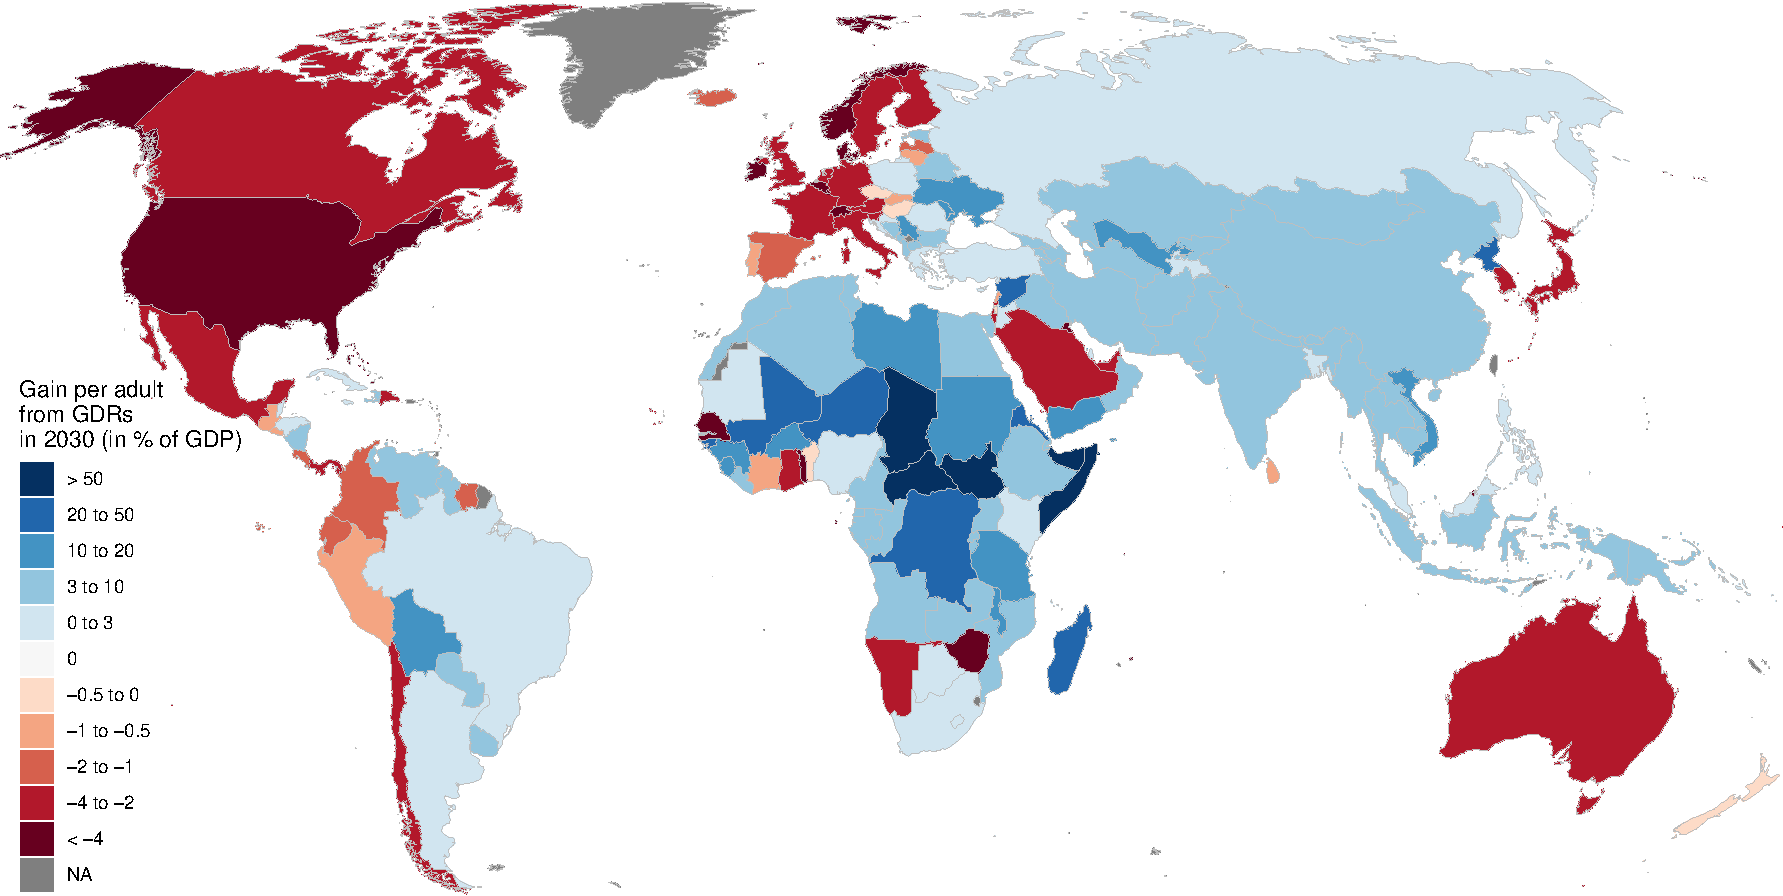
\includegraphics[width=\textwidth]{../figures/maps/gain_gdr_over_gdp_2030.pdf}} 
    {\small \textit{Note:} GDRs are calibrated with the preferred parameters of the \href{https://usfairshare.org/}{U.S. Climate Action Network} \citep{athanasiou_fair_2022} using the Efficiency scenario (2\textdegree{}C with $>$50\% chance) of the Global Energy Assessment \citep{johansson_global_2012} and a price of \$144/tCO$_\text{2}$.}
\end{figure} 

\begin{figure}[h!]
    \caption[Comparison between GDR and equal per capita burden-sharing rules.]{Difference between net gains from Greenhouse Development Rights and equal rights per capita. }\label{fig:diff_gain_gdr_gcs_over_gdp_2030}
    \makebox[\textwidth][c]{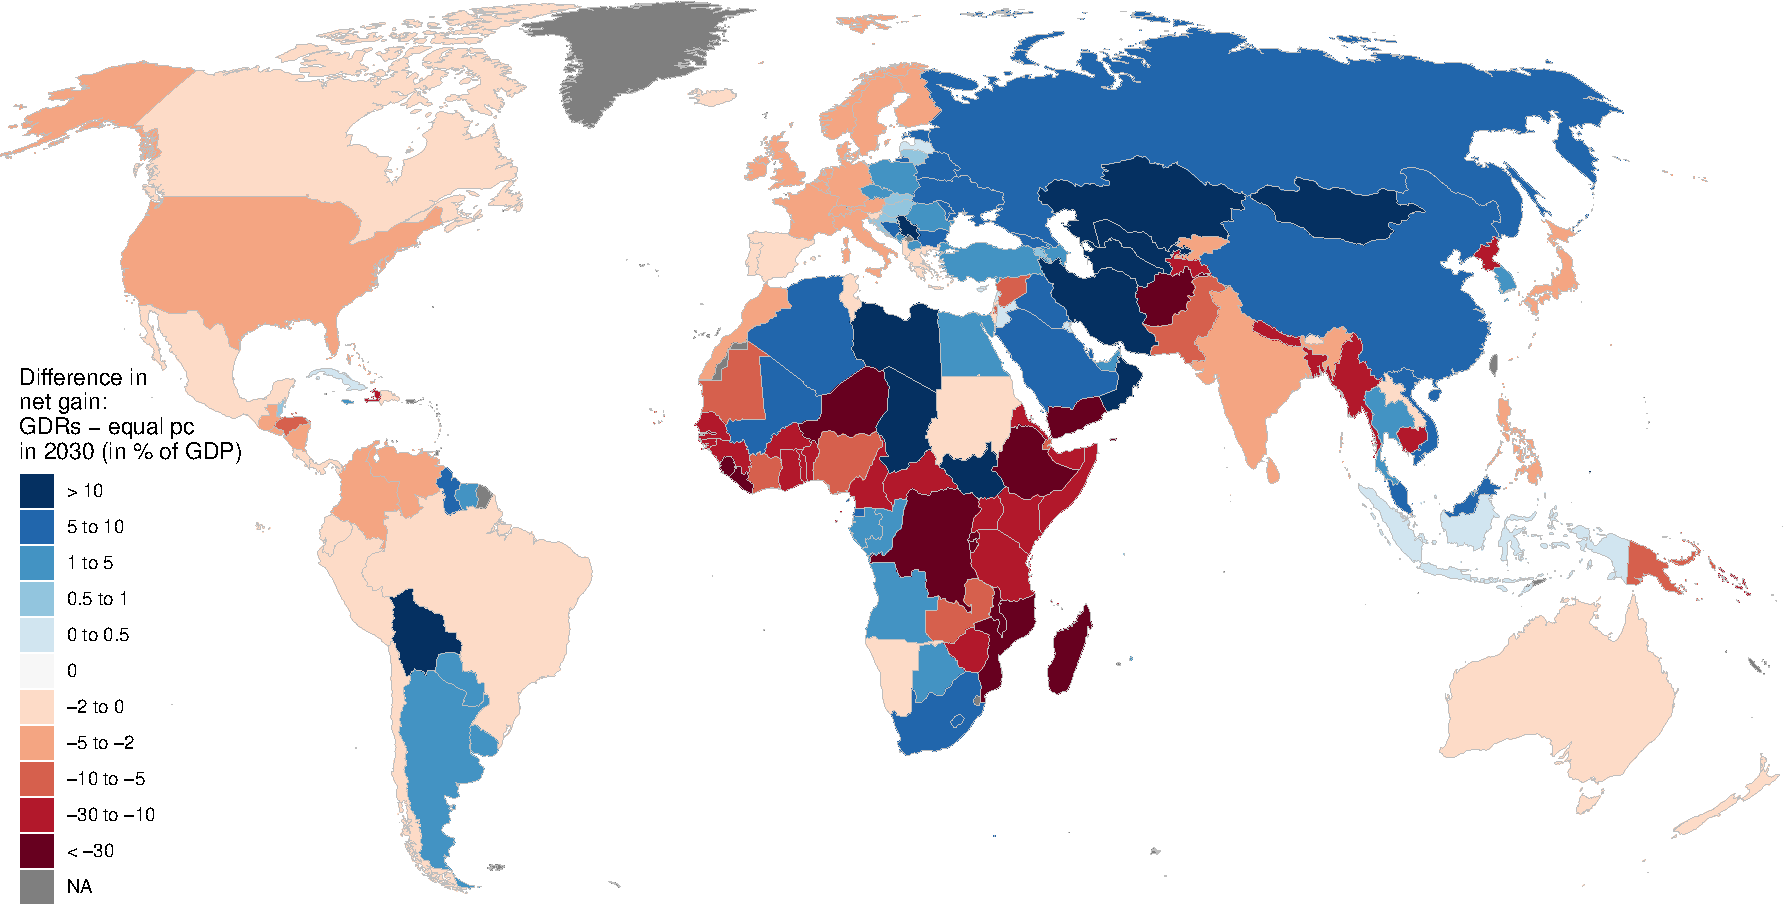
\includegraphics[width=\textwidth]{../figures/maps/diff_gain_gdr_gcs_over_gdp_2030.pdf}} 
    {\small \textit{Note:} GDRs are calibrated with the preferred parameters of the \href{https://usfairshare.org/}{U.S. Climate Action Network} \citep{athanasiou_fair_2022} using the Efficiency scenario (2\textdegree{}C with $>$50\% chance) of the Global Energy Assessment \citep{johansson_global_2012} and a price of \$144/tCO$_\text{2}$.}
\end{figure} % TODO? GDR -> CERF in figure?

\paragraph{Contraction and Convergence.} \citet{meyer_briefing_2004} defines a blend of grandfathering and equal per capita called contraction and convergence (C\&C). This rule grants (tradable) emissions rights to each country, starting at their current emission level and converging linearly to an equal per capita level at some pre-specified date. The \textit{contraction} part comes from the reduction of total emissions rights in line with the climate objective. When discussed around year 2000, the convergence date was specified between 2020 and 2050. This rule, advocated by the Global Commons Institute (a UK think tank), was on the agenda from COP2 to COP15 (in Copenhagen), including at Kyoto, and endorsed by the European Parliament in 1998. More recently, \citet{gignac_allocating_2015} show how C\&C can be made consistent with historical responsibilities, by computing carbon debts and credits until the date of convergence.

\paragraph{Assessments of the NDCs against burden-sharing principles.} 
The regime established by the 2015 Paris agreement to regulate climate change respects none of the burden-sharing principles, and relies instead on voluntary contributions of each country, known as the Nationally Determined Contributions (NDCs). Therefore, a literature (reviewed by \citealp{hohne_regional_2014}) assesses the NDCs against the emissions reduction objective and different burden-sharing principles. \citet{gao_sufficient_2019} expresses the NDCs in terms of emissions in 2030 and infers the rise in temperature implied by the NDCs. \citet{van_den_berg_implications_2020} is the most recent and complete assessment of NDCs against burden-sharing principles (see also \citealp{robiou_du_pont_national_2016,robiou_du_pont_equitable_2017,raupach_sharing_2014}). 

%- Riahi et al. (17), Bauer et al. (17), Van Vuuren et al. (SSP1, 17), Kriegler et al. (SSP5, 16), Fricko et al (SSP2, 17): SSPs => Is SSP5 compatible with RCP2.6? Apparently, according to Riahi not really (Fig. 8) but it still appears in Bauer (Fig. 2) and Yes, according to Kriegler et al (17)
% Scenarios with low emissions:
% - SSP1/2/5-2.6 (or -1.9). (RCP1.9: 1.4°C en 2100 -> 1°C 2300 / 2.6: 1.8 °C -> 1.5 / 4.5: 2.7°C -> 3.3 https://global-climat.com/2021/09/02/rapport-ar6-du-giec-le-point-sur-la-temperature-globale/)
% - Global Energy Assessment (Johansson 12), e.g. Efficiency scenario
% - Greenpeace [Advanced] [R]evolution (Teske 15) 
% - NDCs (Gao et al 19). Check difference SSP2-4.5 with NDCs in 2030. Extend the NDCs either with SSP2 or with some assumption e.g. convergence to SSP2-2.6.
% - Decent Living: Kikstra et al 21
% - Low Energy Demand (Grubler): only has Global North and South
% - IEA ETP17 2DS and B2DS: doesn't have Africa nor GDP nor population
%- https://climateequitymonitor.in/ computes carbon debt based on equal per capita cumulative emissions. contact@climateequitymonitor.in https://twitter.com/equity4climate

% money/CO2 need to meet decent living standards: Kistra et al 21, Hallegatte et al 23 (TODO: read), Millward-Hopkins et al 20, Bruckner et al 22

\subsubsection{Global redistribution}\label{subsubsec:literature_redistribution}
% TODO? Give a stat on income disparities between countries?
% SDG, need for int'l transfers
Addressing global poverty, inequalities and climate change are at the heart of the universally agreed Sustainable Development Goals (SDG). % 12 out of  17
\citet{bolch_arithmetics_2022} have pointed out that low-income countries generally do not have enough domestic resources to eliminate their poverty gap in the short run. %In other words, it would hardly be possible to achieve the first SDG and end extreme poverty by 2030 without international transfers. % Zhang (16) estimates the poverty gap in each country. Global one is at $80G/year.
This shows that international transfers would be needed to rapidly end global poverty. 
%The lack of solidarity from high-income countries has been long criticized. 
In \textit{Beyond the Welfare State}, Gunnar \citet{myrdal_beyond_1960} called for a \textit{welfare world}. He used his Nobel lecture to recommend an increase of foreign aid to low-income countries as ``The type of marginal foreign aid we have provided, is clearly not enough to meet their barest needs'' \citep{myrdal_equality_1975}.

% Unequal exchange, Hickel
Following the labor theory of value, a strand of economists have argued that global inequalities stem from unequal exchange in international trade \citep{arghiri_unequal_1972}. Indeed, the stark disparity in wages between countries implies that one unit of labor exported by an American commands five units of labor embodied in goods imported to the U.S., while Ethiopians need to export 50 units of labor to get one in their imports \citep{alsamawi_employment_2014,reyes_better_2017}.
Taking stock, \citet{hickel_divide_2017} proposes to globally establish minimum wages at 50\% of the local median wage. \citet{hickel_divide_2017} also suggests other solutions against global inequality, which inspired our questionnaire: cancellation of low-income countries' public debt, fair trade (in particular no tariffs from high-income countries, reduced patent protections, reduced farming subsidies in rich countries), measures against tax evasion (e.g. a global financial register), land reform, and a fair international climate policy. 

\citet{piketty_capital_2014} prominently defends a progressive wealth tax at the global level, though he did not specify whether the revenues should fund international transfers. %how the revenues should be used, nor whether there should fund international transfers.% and it was implicit that each country would retain the revenues it collected. 

% Unfairness of current tax rates
\citet{kopczuk_limitations_2005} compute the optimal linear income tax rates for all countries in two ways: globally centralized and decentralized (i.e. in each country, without international transfers). They show that the average decentralized rate is 41\%. The global one 62\%, which would finance a basic income of 250\$/month (higher than 73 countries' GDP per capita). From a current global Gini index of 0.695, they show that decentralized optimal taxation would barely reduce global inequality to 0.69, while global taxation would bring the Gini down to 0.25. Current foreign aid can only be rationalized if the U.S. attaches 2,000 less value to a citizen in poorest countries than to an American (or 1,000 less if half of the transfers are diverted due to corruption). 

% Carthy & Walsh (Oxfam, 22) propose various sources of funding for damages.
% Piketty (2014) "At what rate would [a global wealth tax] be levied? One might imagine a rate of 0 percent for net assets below 1 million euros, 1 percent between 1 and 5 million, and 2 percent above 5 million. Or one might prefer a much more steeply progressive tax on the largest fortunes (for example, a rate of 5 or 10 percent on assets above 1 billion euros). There might also be advantages to having a minimal rate on modest-to-average wealth (for example, 0.1 percent below 200,000 euros and 0.5 percent between 200,000 and 1 million)" He doesn't explicitly talk about revenue use, but implicitly they would be retained by each collecting country: "Le rôle principal de l'impôt sur le capital n'est pas de financer l'État social, mais de réguler le capitalisme.", "En principe, chaque pays de l'Union européenne pourrait obtenir des recettes du même ordre en appliquant seul un tel système."

\subsubsection{Basic income}\label{subsubsec:literature_basic_income}

Unconditional cash transfers (UCT) are increasingly seen as an effective way to end extreme poverty. Indeed, positive results from randomized controlled trials are accumulating: \citet{gangopadhyay_cash_2015} find that UCT outperform a food subsidy; \citet{haushofer_short-term_2016} find significant impacts on health, economic outcomes, and psychological well-being; \citet{egger_general_2022} find large positive spillovers on non-recipient people, and minimal inflation. 
Reviews of extant research confirm the positive outcomes of UCT \citep{standing_little_2014,bastagli_cash_2016}.

Although delivering cash to remote places and avoiding fraud is challenging in regions without a proper civil register, mobile phones could be used as tools for banking and biometric identification \citep{harnett_taking_2017}. While many places are still lacking internet access, progress is rapid in satellite internet access, and some argue that it could soon become cheap and ubiquitous \citep{hanson_satellite_2016}.

\subsubsection{Global democracy}\label{subsubsec:literature_democracy}

The idea of world federalism follows a long tradition, dating back at least to \citet{kant_zum_1795}, who argued that this was the necessary condition for perpetual peace. 
International organizations were eventually created to foster peace, though the League of Nations and its successor, the United Nations, never succeeded in avoiding military conflicts. 
Many have argued that we need stronger and more democratic global institutions, competent to address global challenges like extreme poverty, climate change, wars, pandemics, or financial stability. 
Before World War II, feminist and pacifist \citet{maverick_lloyd_chaos_1937} founded the \textit{Campaign for World Government}, defending direct representation at the global scale. 
\citet{einstein_general_1947} called for the subordination of the UN Security Council to the General Assembly, and the direct election of UN delegates. 
Since 2007, individuals and institutions from more than 150 countries have endorsed the appeal for a United Nations Parliamentary Assembly (UNPA), including 1,800 member of parliament, heads of state, as well the European Parliament, the Pan-African Parliament, and the Latin-American Parliament. The UNPA calls for a gradual implementation of a democratic assembly, starting with a consultative assembly composed of members of national parliaments, allowing for the direction election of its members in voluntary countries, and evolving toward a world parliament able to adopt binding regulations once all members are directly elected \citep{leinen_world_2018}. % READ Ch 13, 21, 22, 26
Besides the UNPA, various scholars have proposed different models of global democracy, ranging from deliberative spaces to a world federation \citep{archibugi_global_2011}. % TODO READ and expand, also read marchetti_global_2008
%Using surveys covering 86\% of global population, \citet{hale_could_2019} find that the world as a whole is less polarized that some countries and argue against the fear people's views would be too diverse for a functioning global democracy. 
While the most radical proposals are still out of sight, an assembly of random citizens representative of the world population has already been convened. It has produced a joint statement at the COP26 \citep{global_assembly_report_2022}, and a similar \textit{World Citizens' Assembly} should soon follow. 
% Stanford dico (kuyper_global_2016)? 

% ___________________________

% Burden-sharing
%- Agarwal & Narain (91) first to defend an equal right to emit per capita (equal to the absorbing capacity of the Earth)
%- Gampfer (14): lab experiment (ultimatum game) to test whether preferences respect fairness principles
%- Chancel & Piketty (15): global progressive carbon tax
% cf. bottom

% Global policies attitudes 
%* ISSP (19): Near consensus that “Present economic differences between rich and poor countries are too large.” p. 102, slight minorities (in rich countries) that “People in wealthy countries should make an additional tax contribution to help people in poor countries.” p. 104, but strong majorities everywhere that “People from poor countries should be allowed to work in wealthy countries.” p. 106
%* Ghassim et al. (22): support for stronger UN with more direct elections.
%* Ghassim (20):  in Germany those two parties that supposedly endorse global democracy – the Greens and the Left – benefitted, gaining nine and three percentage points respectively in terms of voting intentions. Meanwhile, the traditional centrist parties – SPD and CDU – each lost six percentage points due to their supposed opposition to global democracy.
%* Beiser-McGrath & Bernauer (19): Conjoint analysis in US, DE. Variant of carbon tax is 8 (US) - 17 (DE) p.p. more likely to be preferred and 50% more likely to be supported if tax is extended to all industrialized countries (Fig 1, 4). (Unfortunately, don't test extension to global level).
%- Çarkoğlu.. (15) International Social Survey Program 2010 data reveal that people in LDCs are less supportive of international agreements forcing their country to take necessary environmental measures than are citizens in the developed world [80% instead of 85%]. (‘for environmental problems, there should be international agreements that [their country] and other countries should be made to follow.’)
%* Carattini et al. (Nature, 19): 1k in US, IA, ZA, AU, UK. Each respondent receives one variant at random of global carbon price of 40/60/80 $/t redistributed as international dividend / national dividend / mitigation in all countries / mitigation in developing countries / domestic mitigation / reduced labour tax. Immense majorities for any scheme in India, small majorities for each elsewhere except US international dividend (44%) or mitigation in developing (43%), and AU mitigation in developing (49,6%). PB: very low sample size (~167) for a given redistribution, even lower (~55) for a given variant (that also specifies the price). Appendix also contains estimation of distributive impacts. Representative only along the two quotas: gender and age. Don't give the representativeness in terms of income (the third socio-demos that they ask) so it's probably bad.


% Global policies
%* Beyond the welfare state: Myrdal 58
% Pottier et al (17): A survey of global climate justice 
%* Hickel (17): The Divide: A Brief Guide to Global Inequality and its Solutions
%* Kopczuk et al (EER, 17) Compute optimal linear tax rate for all countries in two ways: decentralized or globally. Shows that the tax rate increases with inequality of skills (calibrated with the gini). The average decentralized rate is 0.41 The global one 0.62, with a global demogrant of 250$/month (higher than 73 countries' GDP). Show that within decentralized/country optimal taxation would not decrease global inequality by much (gini from 0.695 to 0.69, but down to 0.25 with global income tax). Show that USA don't give a damn of poor countries' people. citizens in the US (one of the richest) attach only 1/(2,000\*a) of the weight to the welfare of citizens in poorest countries, where a is the share  of transfer (supposedly) effectively arriving to the recipients. e.g. if half of aid is wasted by corrupt politicians, the weight is 1/1000.
% Carthy & Walsh (Oxfam, 22) propose various sources of funding for damages.
% Piketty (2014) "At what rate would [a global wealth tax] be levied? One might imagine a rate of 0 percent for net assets below 1 million euros, 1 percent between 1 and 5 million, and 2 percent above 5 million. Or one might prefer a much more steeply progressive tax on the largest fortunes (for example, a rate of 5 or 10 percent on assets above 1 billion euros). There might also be advantages to having a minimal rate on modest-to-average wealth (for example, 0.1 percent below 200,000 euros and 0.5 percent between 200,000 and 1 million)" He doesn't explicitly talk about revenue use, but implicitly they would be retained by each collecting country: "Le rôle principal de l'impôt sur le capital n'est pas de financer l'État social, mais de réguler le capitalisme.", "En principe, chaque pays de l'Union européenne pourrait obtenir des recettes du même ordre en appliquant seul un tel système."

% Global carbon pricing TODO find current advocates of GCS
%* Grubb (90), Betram (92) advocate for global market with equal pc right
%* Bergh et al. (20) call for a "dual-track transition to global carbon pricing": an expanding climate club, and "a reorientation of UNFCCC negotiations creates room for talking seriously about a global carbon price schedule, including redistribution-of-revenues rules." They don't specify which equity rules to use.
%* Jamieson (01) advocates of equal pc burden-sharing (after the precursors Agarwal & Narain (91))
%* Bear et al (Science, 00), Bear (02), Athanasiou & Baer (02) advocate for equal pc burden-sharing (although weirdly, Bear & Athanasiou then change mind and advocate for the Greenhouse Development Rights, accounting for capacity and responsibility)
%* Cramton et al (17): Livre de pontes. Tout le monde est d'accord : un prix mondial du carbone est requis, il ne peut être obtenu que par la réciprocité des engagements (style climate club), et il faut quelques transferts des riches vers les pauvres ainsi que des sanctions commerciales pour aligner les incitations. Ch 4 (also Cramton et al 15) propose la formule suivante de transfert (positif ou négatif) à un fonds climat : générosité*émissions en excès (par rapport à la cible)*prix du carbone. On demanderait aux États autour de la moyenne d'émission de fixer ce paramètre de générosité, pour qu'il soit fixé de sorte à maximiser le prix, puis on fixerait le prix comme le prix minimum proposé (après avoir éjecté qqs pays récalcitrants des négos). Puis, sanctions commerciales pour ceux qui ne respectent pas le prix. Ch Gollier & Tirole proposent une formule aussi simple que l'autre : quota global*((1-g)*part des émissions à t=0 + g*part de la population), où g joue le même rôle de paramètre de générosité/éthique (que je voudrais mettre à 1, mais qu'ils disent tous de mettre < 1 pour que les pays riches acceptent. Le livre argumente bcp sur prix vs. quantité (TLM préfère prix sauf Gollier & Tirole), l'argument le plus convaincant en faveur du prix c'est qu'avec la procédure proposée le prix négocié serait le plus élevé possible, alors qu'avec la quantité c'est le budget carbone qui serait le point focal et ça aboutirait à une impasse (objectif trop ambitieux).
% Blanchard & Tirole
%* MacKay et al (Nature, 15) summarizes the above
%* Weitzman (17) advocates for a World Climate Assembly, choosing the price level with the median voter, and each country retaining the revenues.
% Fleurbaey & Zuber (13): The discount rate converges to the worst-off (affected by the measure) to the worst-off (beneficiary of the measure) discount rate, which depends on the growth between both agents. Applied to real data, we can consider that the worst-off affected by a global tax on CO_2 is the average-earner on earth (around 75% centile i.e. ~1000€/month, cf. Chancel & Piketty, Lakner & Milanovic, Chakravorty) while the worst-off beneficiary is the worst-off person in the future (among those less affected by CC thanks to the measure), probably below 1000€/month => negative discount rate.
% Stanton (11): Negishi weights obviate the IAMs’ equalization of income. 4 ways to solve this problem: 1. be more transparent, 2. stop weighting, 3. take linear utility (i.e. maximize global GDP), 4. stop optimizing. 
% Hoel (91): Shows that an international tax can be designed so that it is both efficient and satisfies whatever distributional objectives one might have.
% IMF (2019): global pricing (with either differentiated prices or international transfers) or, as a first step, a carbon price floor. 25% of revenues should be rebated to the bottom 40%, the rest used to reduce distortionary taxes or for green investments. Estimate that $75/t is needed in 2030 for 2°C.
% Parry et al (21): Proposal for an International Carbon Price Floor Among Large Emitters. Acknowledges that transfers could be necessary to induce climate action in low/middle-income countries, talks about transferring 1% of carbon revenues.
%- Sager: distributive effects of global pricing without int'l transfers.
%- Budolfson et al. (incl. Fleurbaey, Méjean, Zuber, Dennig) (21): global carbon price with within-country per capita dividend. Acknowledge that "The overall benefits to society are even greater if total carbon tax revenues are returned on an equal per capita basis globally, which directs more of the revenues towards the poorest populations in the world (rather than the poorest within each country or region)." Very short (3p, no appendix, no suppl. info)

% Foreign aid 
%* Kaufmann et al (12) Shows the level of perceived and desired aid in 26 countries between 2005 and 2008 (cf. Table 1). In most countries (incl. UK, DE, FR, ES but not U.S.) desired aid is larger than perceived. Argue that this is due to political influence efforts/possibilities of the rich, as they prefer less aid due to vested interests (support this by a theoretical model + correlations between level of lobbying and actual aid level, controling for desired aid). In most countries the gap between the two is small, except in the U.S. where perceived is 7.5% of GDP and preferred is 3%.Use WVS and Gallup (like Chong & Gradstein, Paxton & Knack) but have more waves and the others don't use the question on perceived aid. Shows that richer want less aid ("those in the top income quintile favour ODA (as a share of GNI) that is 0.13 percentage points lower than the preferred share for individuals in the bottom 40\% of the income distribution" after controling for perceived aid - our regression results are sensibly the same.). from 0 to higher than 25%: threshold at 0.05; 0.15; 0.35; 0.75; 1.5; 2.5; 4; 7.5; 17.5; 25, i.e. same number of thresholds but small than ours below 2.5 and higher above. 
%*? Milner & Tingley (13): (highly cited but no original data, don't think we need to cite it) In 2008, 44% of American wanted foreign aid cut (american elections study, 08). fraction of federal budget going to foreign aid (mean: 27%, median: 25%) / should go (mean: 13%, median: 10%) (WorldPublicOpinion, 10)
% PIPA (01): Overwhelming majorities support a multilateral effort to cut hunger in half by the year 2015 and say that they would be willing to pay for the costs of such a program. However, most do not think that the average American would be as willing to pay the necessary costs. when PIPA asked respondents to estimate how much of the federal budget was devoted to foreign aid, the median estimate was 15% -- 15 times the actual amount, which was just under 1%. More dramatically, when asked what an appropriate percentage would be, the median response was 5% -- 5 times the actual amount. And when asked to imagine that they heard the real amount was only 1%, only 18% of respondents said they thought that would be too much--as compared to the 75% who had initially said that the US was spending too much. what percentage of their "tax dollars that go to help poor people at home and abroad...should go to help poor people in other countries." The mean response was 16% (down a bit from 22% in response to this question in a 1996 PIPA poll). Strikingly, this turns out to be a far higher percentage than is currently given. In 1999, a bit less than 4% of the total spent on the poor went to the poor abroad. Sixty percent of respondents proposed a percentage that was higher than 4%.
%- DFID (10): Priorities: 1 NHS, 2 education, 3 support to poor countries, 4 police, 5 defence (p. 19). Show majority support for increased aid until 07, then median is to support stable aid (due to crisis?). It seems they don't give the info on actual amount though.
%* PIPA (08): Across 20 countries, 81% support that "developed countries have a moral responsibility to help reduce hunger ansevere poverty in poor countries (majority in every country). “the World Bank (Shantayanan et al, 2002) has estimated that it will require an extra US$39-54 billion per year to meet Millennium Development Goal 1 (MDG1). (…) The per person cost of meeting MDG1 came to £25 for the UK, $56 for the US, €27 for Germany, and so on. On average 77 per cent of respondents are in favour of contributing towards meeting the goal (provided that all others do too). To take the US example, 75 per cent of people supported paying an extra $56 per year to meet MDG1. What is significant about this figure is that it is only slightly below the support for the ‘cost free’ question as to whether the US should be willing to share a  small portion of its wealth with those who are in great need (79%).” Hudson & van Heerde (12)
%* Hudson & van Heerde (12):Reviews literature on foreign aid and criticizes it on a number of points (e.g. not uncovering the determinants, and not asking well the questions). Shows strong support for poverty alleviation, (at least partly) out of intrinsic altruism. Use 4 main sources: PIPA (01, 08) UK DIDP, Eurobarometer; cf. Table 1 for all surveys on foreign aid / Public support for development has been famously described as a mile wide and and inch deep (Smillie, 1996: ref impossible to find). Hard times at home have meant that public support appears to have turned against international development efforts (Henson and Lindstrom, 2010). / Monitor public support: (Fransman and Solignac Lacomte, 2004; McDonnell et al, 2003), Paxton and Knack, 2008; Chong & Gradstein 2006. Review surveys on aid. / ~75% support aid in developed countries (stable) but ‘84 per cent agreed with the assertion that ‘taking care of problems at home is more important than giving aid to foreign countries’ (PIPA, 2001:9).” / References on covariates of aid support / PIPA 2001, "On average, Americans thought just under 25 per cent of the US budget was allocated to foreign aid, and government should allocate less than 14 per cent of the national budget. However, when told that US spends approximately 1 per cent of the federal budget on foreign aid, 37 per cent of respondents thought this was too little, 44 per cent thought it was about right, and 13 per cent thought it too much."  Think that only 23% of aid really goes to the poor / “The 2009 UK survey, Public Attitudes towards Development, reports ‘public support for overseas aid’ at 72 per cent (DFID, 2009); while in the US support was a comparable 79 per cent (PIPA, 2001); and average support across the EU trends slightly higher than in the US and UK with 91 per cent saying it was either very (53%) or fairly (38%) important to provide aid to poor countries (Eurobarometer, 2005).” / “DFID has now begun asking questions that provide relative measures of the salience of development aid vis-à-vis other competing policy issues (DFID, 2009; IDC, 2009). / "high proportion (61%) of US citizens who felt that the US spends too much on foreign aid. [from another source]” / “The distinction between foreign aid, which includes military spending, and development aid/assistance is an important one” / “81 per cent of respondents believed that developed countries do have a moral responsibility to work towards reducing hunger and severe poverty (WorldPublicOpinion.org, 2008). (…) there are a good number of people who support aid despite the fact they do not think it works. What this suggests – but cannot show in any detail – is that people have nonutilitarian motives for supporting aid.” / “support for development assistance is highly contingent on respondents’ perceptions of the effectiveness of aid, especially with regard to corruption (Henson et al, 2010). For example, in the UK, 47 per cent of respondents thought that aid was wasted, with sizable majorities citing corruption and poor management and/or delivery as primary factors (DFID, 2008). More disconcertingly, US respondents thought that only 23 per cent of US aid money that goes to poor countries ends up helping the people who really need it and 54 per cent of US aid money that goes to poor countries ends up in the pockets of corrupt government officials (PIPA, 2001). (…) international charities and NGOs are deemed best suited/most effective compared to donor countries” / UK ‘MyAid’ plan – where the public gets to vote on how a pot of money should be distributed – / "public engagement should be about ‘opening up the political and wider societal space to the possibility of deeper change’ (Darnton and Kirk, 2011:14).”
%* Gilens (01) 17% fewer American with high political knowledge want to cut foreign aid when we provide them specific information about aid amount.
%- Chong & Gradstein (16): from WVS 95-99, 58% want that their country give more foreign aid (but misperceptions are not taken into account)
%* Bauhr et al (13): Support for aid is reduced by perception of corruption in recipient countries. However, this effect is reduced by the aid-corruption paradox (and other things): most corrupt countries need more help.
%- Nair (18): (lack of) Aid support in US driven by information on global distribution, because people underestimate their rank by 27 centiles and overestimate global median income by a factor 10.
%- Williamson (19): Public Ignorance or Elitist Jargon? Reconsidering Americans’ Overestimates of Government Waste and Foreign Aid. "Foreign aid" encompasses military spending, in the mind of American.
%- McDonnell et al (03) Public Opinion and the Fight against Poverty
%- Nair (16): preferences driven by worldviews rather than self-interest
%- Bodenstein & Faust (17): Determinants of support for aid conditionality. They are: perceived corruption in donor country, right-wing.
%- Scotto et al (17): We Spend How Much? Misperceptions, Innumeracy, and Support for the Foreign Aid in the United States and Great Britain. Less American and British want aid cut when information on current aid is given in % of GDP rather than in $.
%* Paxton & Knack (12): Majorities want more aid, and main determinants are trust, ideology, interest in politics, and female (all positive). Gallup 02: in US 45% want more aid (rather than stable) vs. 68-91 in DE-UK-ES. Like Chong & Gradstein, find that desired aid increases with income, contrary to Kaufmann et al. but the latter contains more datasets.
%- Wood (15): Determinants for aid support in Australia. Wood (18) Examine Australian support for aid: although there is support to help foreign poor, people back recent aid cuts.
%- Bayram (17): Aid support associated with trust, i.e. seeing integrity and trustworthiness in others.
%- Cheng & Smyth (16): Why Give it Away When You Need it Yourself? Understanding Public Support for Foreign Aid in China. Political ideology and patriotism main explaining variables for aid support. People in poorer provinces less supportive.
%- Milner & Tingley (10) theory + empirics: who supports aid and why. owners of capital in donor countries tend to gain from aid and thus are more likely to support giving aid
%- Easterly (JEP, 03) Can Foreign Aid Buy Growth? No (disproves Hansen & Tarp).
%- Hansen & Tarp (01) Aid increases growth (empirical evidence)
%- Tresch et al. (22): 66% of Swiss people want to increase their foreign aid; also Borofsky
%- Harris (17): majority of French want to decrease foreign aid


% Universalism
%- Enke et al. (Manag. Science, 23): measures universalism by asking to split donation to domestic and foreigner of same absolute income (US).
%- Enke et al. (ReStud, 23): unviersalism more correlated to policy attitudes than income, education, religiosity or beliefs about government efficiency (West).
%- Cappelen et al. (NBER, 22): how unviversalism (as measured above) varies across countries. Comparable in Europe and US (lower in China, higher in Africa)
%- Cherry et al (17) show in the lab that some people prefer policies detrimental to them due to their worldview.


% Free-riding
%- Mildenberg (2019): people are not free riders
%- McGrath & Bernauer (17): review paper. people are not free riders. Preferences concerning climate policy tend to be driven primarily by a range of personal predispositions and cost considerations, which existing research has already explored quite extensively, rather than by considerations of what other countries do
%- Bernauer & Gampfer (15): US and IA people are not free riders. They each overestimate their country's emissions at one third of global total.


% Social norms
%- Bursztyn et al. (AER, 20): social norms can change following new public information such as unexpected election outcome. After Trump election, people express more xenophobic views and judge less severely those who do.
%- Farrow et al. (17): review of effect of social norm intervention on environmental attitudes

% Incentive compatibility
%- Danz et al


% Second-order beliefs
%* Mildenberg & Tingley (19): survey elites (Congress staffers, scholars) and public in U.S. and China and show pluralistic ignorance of pro-climate attitudes, egocentric bias, and increasing support after beliefs are updated.
%- Bursztyn & Yang (21): Review of the field. Misperceptions about others are widespread, asymmetric, much larger when about out-group members, and positively associated with one’s own attitudes.
%- Drews et al. (22): in Spain, supporters (resp. opponents) of carbon tax overestimate (resp. underestimate) support. Providing information doesn't change the overall support.
%* Falk et al. (21): Respondents vastly underestimate the prevalence of climate- friendly behaviors and norms among their fellow citizens. Providing respondents with correct information causally raises individual willingness to fight climate change as well as individual support for climate policies. The effects are strongest for individuals who are skeptical about the existence and threat of global warming.
%- Di Tella et al. (AER, 15): The results of the lab experiment favor the hypothesis that people avoid altruistic actions by distorting beliefs about others' altruism
%- Allport (1924): first book on pluralistic ignorance
%- Allport (40): function of poll is to correct pluralistic ignorance
%- Studies on pluralistic ignorance: business (Buckley et al. 00), against affirmative action (Van Boven 00), political correctness (Braghieri, AER 21), alcohol (Suls & Green, 03), white support for racial segregation (O'Gorman 75), CC (Geiger & Swim 16), hooking up (Lambert et al 03, cf. note for paragraph of pluralistic ignorance), women working outside home in Saudi Arabia (Bursztyn et al. 20)
%- Geiger & Swim (16) Shows that pluralistic ignorance of others' concern about CC leads people to talk less about CC and self-silence themselves.
%- Miller & MacFarland (87) Shows that pluralistic ignorance emerges because individuals believe that fear of embarrassment is a sufficient cause for their own behavior but not for the behavior of others.


% Elite surveys TODO find more
%* Mildenberg & Tingley (19): Congress staffers, cf. second-order beliefs
%- Hertel-Fernandez et al. (2019): Survey on US Congress staffers (not on climate)
%- Milner & Tingley (10) (not sure it's a survey) owners of capital in donor countries tend to gain from aid and thus are more likely to support giving aid
%- Lange et al. (Energy Econ, 2007): climate negotiators
%- Lange et al. (EER, 2010): same data as Lange et al. (10)
%- Dannenberg et al. (ERE, 2010): elicit climate negotiators’ equity preferences using Fehr & Schmidt (99) method => regional differences in addressing climate change are driven more by national interests than by different equity concerns
%- Kesternich et al. (EEPS, 2020): survey on climate negotiators about their preferred burden-sharing rules: we observe tendencies for a more harmonized view among key groups towards the ability-to-pay rule in a setting of weighted burden sharing rules
%- Lange & Schwirplies (ERE, 2017): combines Lange et al. (10) and Schleich et al.
%* Hjerpe et al. (2011): Delegates at COP2009. The results indicate that voluntary contribution, indicated as willingness to contribute, was the least preferred principle among both negotiators and observers. Three of the four principles for allocating mitigation commitments were recognized widely across the major geographical regions: historic 1990, capacity to pay, and equal per capita emissions. The difference was never below 25 percentage units, and the opponent share never exceeded 16%.
%- Scholte et al. (2020)
%- Bayram (17): cosmopolitanism of German politicians and their respect of international law


% Global poverty gap
%* Bolch et al. (22)
%- Zhang (16) estimates the poverty gap in each country. Global one is at $80G/year.


% Basic income 
%* Egger et al. (19): positive gen eq effects. We provided one-time cash transfers of about USD 1000 to over 10,500 poor households across 653 randomized villages in rural Kenya. The implied fiscal shock was over 15 percent of local GDP. We find large impacts on consumption and assets for recipients. Importantly, we document large positive spillovers on non-recipient households and firms, and minimal price inflation.
%* Haushofer & Shapiro (16): The Short-term Impact of Unconditional Cash Transfers to the Poor: Experimental Evidence from Kenya. Monthly transfers are more likely than lump-sum transfers to improve food security


% Unequal exchange / embodided labour
%- Reyes et al (17)
%- Sakai et al (17)
%- Alsamawi et al. 2014


% NDCs assessments or burden-sharing computations. 
%- Bourban (18): Soutient un marché du carbone avec droits en proportion des émissions cumulées depuis 1990. Et des “mesures volontaires de contrôle de la population mondiale”.
%- Raupach et al (NCC, 14): clear computations of regional carbon budget under different budget sharing
%- van den Berg et al (20): same
%- Meyer (04) Contraction and Convergence (i.e. grandfathering converging to equal pc, within an ETS)
%- AGBM 97: Contraction and Convergence proposed by France
%- >Baer et al (08)< (cite this one, others don't give more info), Baer (13), Athanasiou et al (22), Holz et al (19) https://calculator.climateequityreference.org/ Athanasiou, Greenhouse Development Rights, EcoEquity calculator, US fair share. Effort-sharing approach based on splitting emissions reductions in function of capacity to pay (~ share of global income in top 30%) and responsibility (share of emissions since 1950), weighted equally. Corresponds to UNFCCC wording. Pb of this method (applying to any choice of parameters): A country with relatively low incomes (e.g. equal distribution slightly above the p70) and that has few historical responsibility would have a relatively low effort. Even more problematic, the **poorest countries would have virtually 0% of the effort, hence they would be allowed to emit following the baseline trajectory… but this baseline is not fair; it amounts to grandfathering**. It is computed as the “product of the projected GDP and CO2 emission intensity”. ([https://climateequityreference.org/calculator-information/gdp-and-emissions-baselines/](https://climateequityreference.org/calculator-information/gdp-and-emissions-baselines/)), and give for example 0.8tCO2e/cap for RDC in 2030 (16% more than in 2020, but lot lower than the objective of ~4t). => Compared to an equal right to emit pc, this method favors countries like China (allowed to remain stable over 2020-30 vs. reduced by 35-40%) and penalizes countries like the U.S. and Africa. 
%  in Athanasiou et al (22) Justification of Greenhouse Development Rights instead of Equal per capita right is on p. 36. It is weak, and basically that historical responsibility should be taken into account. Conversely, justification against historical resp. is that the latter doesn’t take into account capacity to pay (it is not said like this, but we can think of ex-USSR).
%- Pachauri et al. (Science, 2022): "we find that distributive justice considerations in global climate mitigation will require substantial interregional finance flows" READ
%- Robiou du Pont et al. (NCC, 2017): China’s Nationally Determined Contribution (NDC) is weaker than any of the five equity approaches, India’s and the USA’s NDC are aligned with two, and the EU’s with three. … If the G8 and China adopt the average of the five approaches, the gap between conditional INDCs and 2 C-consistent pathways could be closed.
%- Robiou du Pont et al. (ERL, 2016): READ we identify global cost-optimal emissions scenarios from Integrated Assessment Models that match the G7 agreement [of reducing emissions by ~65% by 2050 compared to 2010, in line with >66% <2°C]. These scenarios have global 2030 emissions targets of 11%–43% below 2010, global net negativeCO2 emissions starting between 2056 and 2080 … G7 members’ Intended Nationally Determined Contribution (INDCs) mitigation targets are in line with a grandfathering approach but lack ambition to meet various visions of climate justice. The INDCs of China and Russia fall short of meeting the requirements of any allocation approach. Depending on how their INDCs are evaluated, the INDCs of India and Brazil can match some equity approaches evaluated in this study.
%- Höhne et al. (Climate Policy, 2014): review of 40 papers READ
%- Gao et al. (FEM, 2019): assesses NDCs
%- Gignac & Matthews (ERL, 15) READ
%- Matthews (16) Quantifying carbon debts among nations 
%- https://climateequitymonitor.in/ computes carbon debt based on equal per capita cumulative emissions. contact@climateequitymonitor.in https://twitter.com/equity4climate


% Mismatch between preferences and climate action TODO! cite
%- McCright & Dunlap (03) show that it's an organized conservative movement that succeeded in the U.S. not ratifying Kyoto, through lobbying and disinformation.


% Wealth tax attitudes
% look for surveys on global tax => I've found no result with survey or attitudes + "global tax" or "global wealth tax" in google scholar
% Fisman et al (17): Americans want a 3% tax on inherited wealth
%- Christensen et al. (Oxfam, 23) p. 32 gives references on rich tax attitudes, with always strong majority support:
%* OECD (19): 52-80% of absolute support for "government tax the rich more than they currently do in order to support the poor" in 21 OECD countries
%* Isbell (22): 34 African countries
%- Patriotic Millionaires (22), UK
%- Americans for Tax Fairness (21), US
%- Gallup (22), US
%- Fight Inequality Alliance India (22), IA

% Different framing of burden-sharing, depending on what should be split:
% - mitigation costs: this is the most used as it is easiest to explain. The issue is that it is not specified how agents pay (or if some agents receive payments) and implicitly, there is no negative costs (transfers exceeding the costs) and the carbon price is not uniform. Used in .
% - emission: this one is vague as it doesn't state at which date emissions pc converge (if they do) and whether there are side payments.
% - emission rights: this one is the most accurate as there is no need of a BAU scenario to compute the mitigation needed and its cost.

% Different fairness principles:
% - equal emission right per capita: using this as a baseline, we can call 'grandfathering' any principle that is more regressive and 'historical responsibility' any principle that is more progressive
% - equal emission reduction (in share of current emission) per capita: grandfathering
% - emission rights proportional to current emissions: grandfathering
% - costs proportional to current emissions: polluter-pay principle
% - costs proportional to cumulative emissions: so-called historical responsibility but may actually have a grandfathering component

% Surveys of population:
% - Schleich et al. (Climate Policy, 16) ask for ranking and find an identical ranking of fairness principles in China, Germany, and the US: accountability (costs according to emissions) followed by capability (according to economic strength), egalitarianism (equal emission per capita), and sovereignty (constant share of global emission) (see Lange & Schiwplies (17) for the computations). 
%   Polluter-pays: Every country has to bear costs according to the emissions it causes (hence countries causing higher emissions have a higher share of the costs).
%   Ability-to-pay: Every country has to bear costs according to its economic strength (hence richer countries have a higher share of the costs).
%   Egalitarian: Every country is allowed to produce the same amount of emissions per capita (hence countries with currently high emissions per capita have higher costs).
%   Sovereignty: Every country is allowed to produce the same share of global emissions as in the past (hence the proportional reduction of emissions is the same for every country).
% other findings: international agreements are important but current ones are unsuccessful, people find themselves poorly represented in climate negotiations
% - Bechtel & Scheve (PNAS, 13) find with a conjoint analysis on FR, DE, UK, US that a climate agreement is 5 p.p. less likely to be preferred (to a random alternative) if only rich countries pay (other burden-sharing are: pay prop. to current emissions / historical emissions / rich countries pay more than poor countries) and 15 p.p. more likely to be preferred if it includes 160 (out of 192) countries rather than 20 => confirms preference for global policies (rather than only partial coverage). Finds that costs is what matters most: preference decreases by 30pp if it’s 2.5% of GDP compared to 0.5%.
% - Carlsson et al. (REE, 13) find using a 09 choice experiment that Americans prefer capacity to pay > current responsibility > historical responsibility > equal emissions per capita while Chinese prefer historical > capacity > current > equal emissions.
%   Capacity to pay: Countries with high income levels must pay a larger share of the costs than countries with low income levels. This option says that countries with greater ability to pay should pay more
%   Current responsibility: Countries with currently high emissions levels must pay a larger share of the costs than countries with currently low emissions levels. This option says that those countries that are currently a larger part of the problem should pay more.
%   Historical responsibility: Countries with a history of high emissions levels must pay a larger share of the costs than countries with a history of lower emissions. This option recognizes that CO2 builds up in the atmosphere over many years. Thus, countries with a history of high emissions should pay more because they caused more of the problem.
%   Equal emissions pc: Countries with emissions per person greater than an agreed amount must pay, and they must pay more the higher their emissions per person area.
% > "equal emissions" is a misnomer as this is about costs (not emissions) and it's just a more progressive version of current responsibility / polluter-pay, where high-emitting pay more and low-emitting don't pay. The result for US is compatible with the other papers as Americans agree that rich countries (or high-emitting, the diff is small) should pay more. The Chinese position could also be reconciliable once we define responsibility from footprint rather than territorial and that there will be transfers from rich to poor countries.
% - Carlsson et al. (Ecol Eco, 11) find that Swedes prefer that "all countries are allowed to emit an equal amount per capita" rather than options where emissions reduce in relation to current or historical emissions and continue to be higher in high-emitting countries. 
% - Meilland et al. (23) find that in US and France, most favored fairness principle is Equality in per capita emissions: "all countries commit to converge to the same average of total emissions per inhabitant, compatible with a controlled climate change" and second-most (which closely follows) is grandfathering: "all countries commit to reduce their emissions by a same proportion". 73% in each disagree with grandfathering when defined as "countries which emitted a lot of carbon in the past have a right to continue emitting more than others in the future". To rationalize these contrasted views with grandfathering, we can interpret them as: equal rights, equal emission reductions, and transfers. 
%   convergence per capita (70%): all countries commit to converge to the same average of total emissions per inhabitant, compatible with a controlled climate change
%   grandfathering (60%): all countries commit to reduce their emissions by a same proportion
%   past emissions (20% choose it among their two favorite): countries which emitted less in the past commit to reduce their emissions less than other countries
%   poor countries (20%): poorer countries commit to reduce their emissions less than richer countries
%   cost-efficiency (20%): countries where reducing emissions is more costly commit to reduce their emissions less than other countries
% Other findings: people prefer international settlement on CC even if it empedes on sovereignty, a majority prefers to target footprint rather than territorial emissions, median is that countries should be held accountable for post-1990 emissions, self-serving bias when judging e.g. India vs. EU, no shared understanding of fairness when asked to coordinate between French and Americans
% - Dechezleprêtre et al. (WP, 22) find that equal per capita right > historical responsability, capabilities > grandfathering; that global CC policies are needed; 50% support for global T&D; strong support for global tax on millionaires; no free-riding. 
% - Dabla-Norris et al. (WP, 23) find strong majority for “all countries” everywhere in “Which countries do you think should be paying to reduce carbon emissions?”, and majority for current rather than historical in all countries but China and Saudi Arabia in “Should countries be paying to reduce carbon emissions based on their current or accumulated historic levels of emissions?”

% > Position making all this compatible: people want that every country engage in strong decarbonization effort together, with a global quota, converging to climate neutrality in the medium run, based on an equal right to emit per person, implying that rich countries pay and low-emitting countries receive funding. Where the rankings differ, it is likely because the definitions or wordings are different, and also because it involves different countries (Sweden != US != China).
% - Schleich find support for costs according to emissions and against immediate equalization of emissions (but nothing against convergence to equal emissions per capita).
% - This is just in contradiction with Carlsson (11) which finds that Swedes prefer the equalization (with a similar wording) to other reduction options. 
% - Bechtel find agreement that rich countries should pay more and historical emissions matter, but just that they should not be the only one to make the efforts. 
% - Carlsson (13) find that the least preferred option in China and US is when low-emitting countries don't participate to the effort. Ability to pay is liked in both countries.
% - Meilland find that convergence is the most preferred, followed by emission reductions of same proportion, disagreement with grandfathering expressed in terms of emission rights.
% - Dechezleprêtre find support for equal right is strongest, although historical responsibility and capabilities are also supported. The quota system is strongly supported.

% Surveys of negotiators:
% - Hjerpe et al. (WP, 11)
% - Dannenberg et al. (ERE, 10): measuring negotiators' equity preferences, regional differences in addressing climate change are driven more by national interests than by different equity concerns.
% - Lange et al. (Energy Econ, 07): Mix of self-serving bias and support for egalitarian principle.
% - Kesternich et al. (EEPS, 21): kind of convergence on ability-to-pay.

% Other papers:
% - Lange & Schwirplies (ERE, 17) develop a theoretical model (building on Buchholz et al. (05)), supported by data, justifying that climate negotiators (chosen by the citizens) have lower environmental preferences than their citizens and equity views more aligned with the other negotiators. 
% - List experiment: Kuklinski et al. 97 or https://blogs.lse.ac.uk/europpblog/2022/04/06/do-russians-tell-the-truth-when-they-say-they-support-the-war-in-ukraine-evidence-from-a-list-experiment/
% % \clearpage
% % \section{Raw results% from the complementary surveys
% % }\label{app:raw_results}
% \clearpage
\section{Raw results% from the complementary surveys
}\label{app:raw_results}
% /!\ Do not replace by app_desc_stats_US1 as the latter also contains figures that are already in the main text

Country-specific raw results are also available as supplementary material files:  \href{https://github.com/bixiou/global_tax_attitudes/raw/main/paper/app_desc_stats_US.pdf}{US}, \href{https://github.com/bixiou/global_tax_attitudes/raw/main/paper/app_desc_stats_EU.pdf}{EU}, \href{https://github.com/bixiou/global_tax_attitudes/raw/main/paper/app_desc_stats_FR.pdf}{FR}, \href{https://github.com/bixiou/global_tax_attitudes/raw/main/paper/app_desc_stats_DE.pdf}{DE}, \href{https://github.com/bixiou/global_tax_attitudes/raw/main/paper/app_desc_stats_ES.pdf}{ES}, \href{https://github.com/bixiou/global_tax_attitudes/raw/main/paper/app_desc_stats_UK.pdf}{UK}.

\begin{figure}[h!]
    \caption[Absolute support for global climate policies]{Absolute support for global climate policies. \\ Share of \textit{Somewhat} or \textit{Strongly support} (in percent, $n$ = 40,680). The color blue denotes an absolute majority. See Figure \ref{fig:oecd} for the relative support. (Questions \ref{q:scale}-\ref{q:millionaire_tax})} 
    \makebox[\textwidth][c]{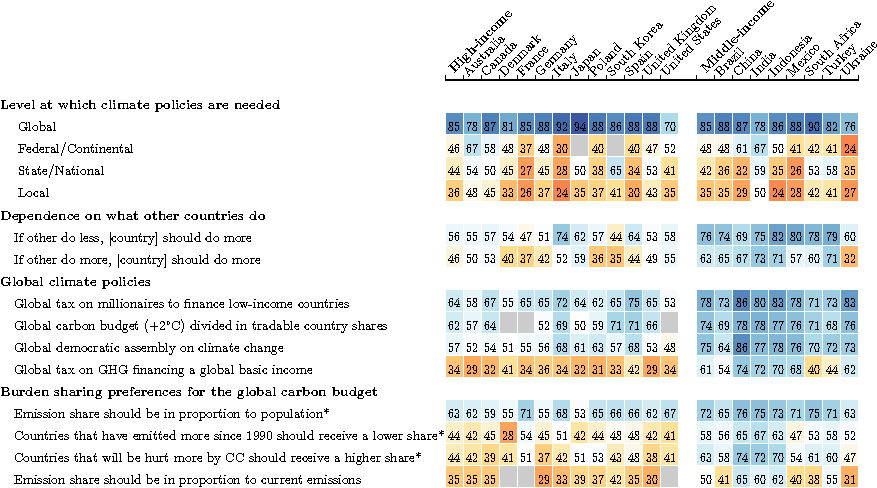
\includegraphics[width=1.2\textwidth]{../figures/OECD/Heatplot_burden_share_all_positive_countries.pdf}}\label{fig:oecd_absolute}
    {\footnotesize *In Denmark, France and the U.S., the questions with an asterisk were asked differently, cf. Question \ref{q:burden_sharing_asterisk}. } 
\end{figure}

\begin{figure}[h!]
    \caption[Comprehension]{Correct answers to comprehension questions (in percent). (Questions \ref{q:understood_gcs}-\ref{q:understood_both})}\label{fig:understood_each}
    \makebox[\textwidth][c]{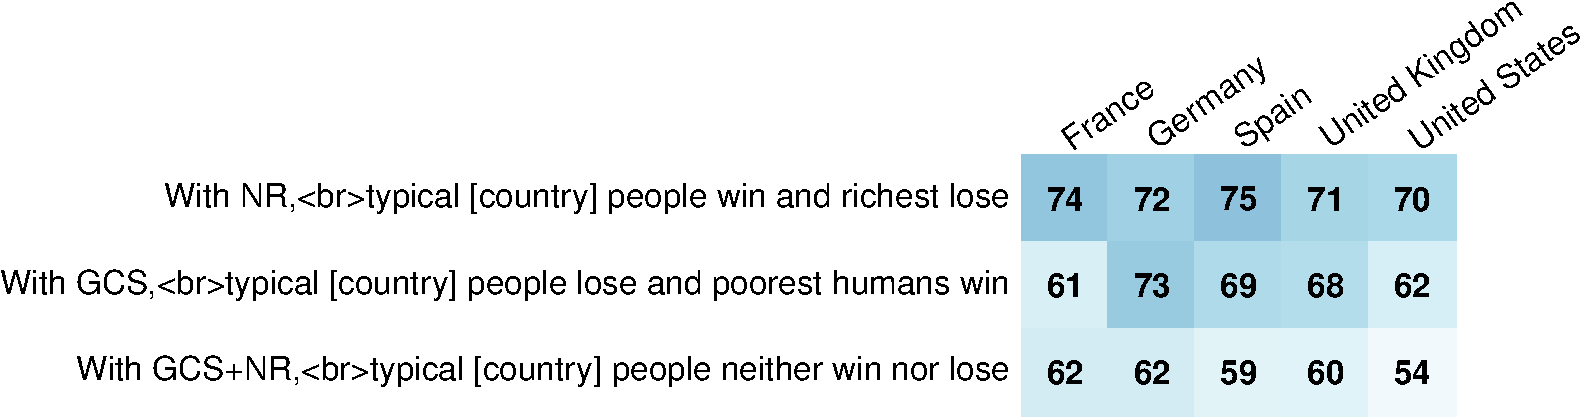
\includegraphics[width=\textwidth]{../figures/country_comparison/understood_each_positive.pdf}} 
\end{figure}

\begin{figure}[h!]
    \caption[Comprehension score]{Number of correct answers to comprehension questions (mean). (Questions \ref{q:understood_gcs}-\ref{q:understood_both})}\label{fig:understood_score}
    \makebox[\textwidth][c]{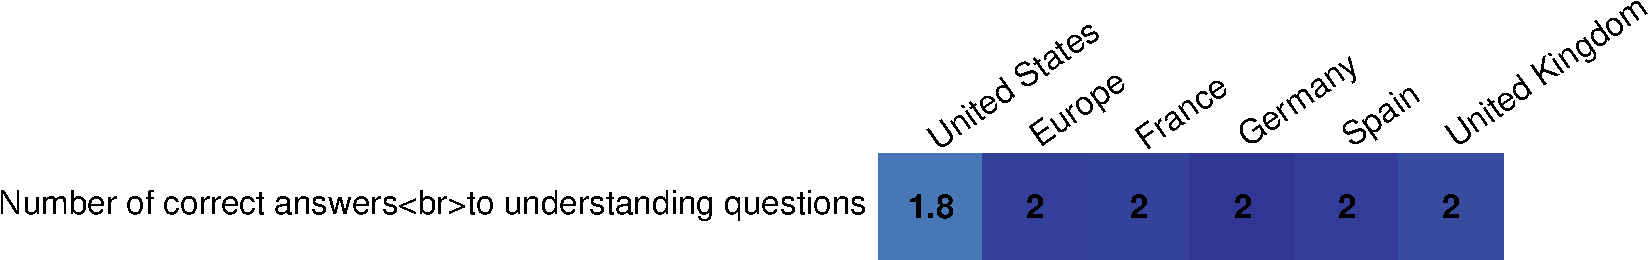
\includegraphics[width=\textwidth]{../figures/country_comparison/understood_score_mean.pdf}} 
\end{figure}

% \begin{figure}[h!]
%     \caption[Support for the Global Climate Scheme]{Support for the GCS, NR and the combination of GCS, NR and C. (Questions \ref{q:gcs_support}, \ref{q:nr_support} and \ref{q:crg_support})}\label{fig:support_binary}
%     \makebox[\textwidth][c]{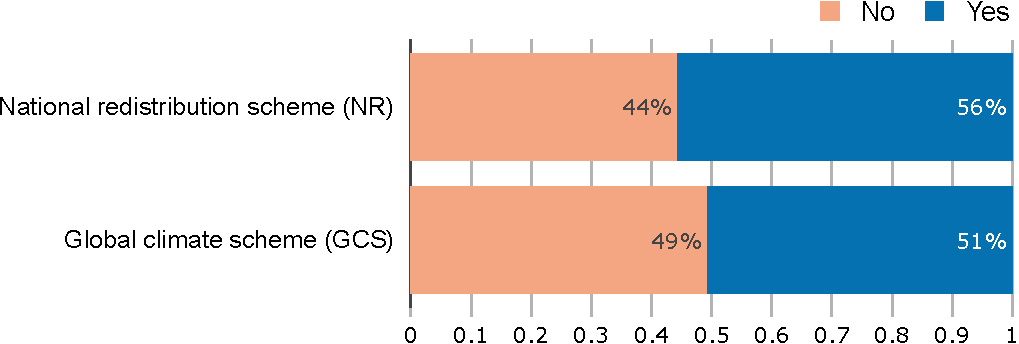
\includegraphics[width=.9\textwidth]{../figures/country_comparison/support_binary.pdf}} 
% \end{figure}

% \begin{figure}[h!]
%     \caption[Beliefs about support for the GCS and NR]{Beliefs regarding the support for the GCS and NR. (Questions \ref{q:gcs_belief} and \ref{q:nr_belief})}\label{fig:belief}
%     \makebox[\textwidth][c]{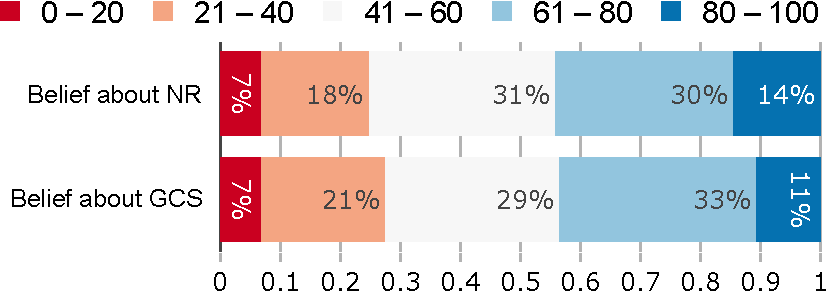
\includegraphics[width=.8\textwidth]{../figures/country_comparison/belief.pdf}} 
% \end{figure}

\begin{figure}[h!]
    \caption[List experiment]{List experiment: mean number of supported policies. (Section \ref{subsubsec:list_exp}, Question \ref{q:list_exp})}\label{fig:list_exp}
    \makebox[\textwidth][c]{
\includegraphics[width=.7\textwidth]{../figures/country_comparison/list_exp_mean.pdf}} 
\end{figure}

\begin{figure}[h!]
    \caption[Conjoint analyses 1 and 2]{Conjoint analyses 1 and 2. (Section \ref{subsubsec:conjoint}, Questions \ref{q:conjoint_a}-\ref{q:conjoint_b})}\label{fig:conjoint}
    \makebox[\textwidth][c]{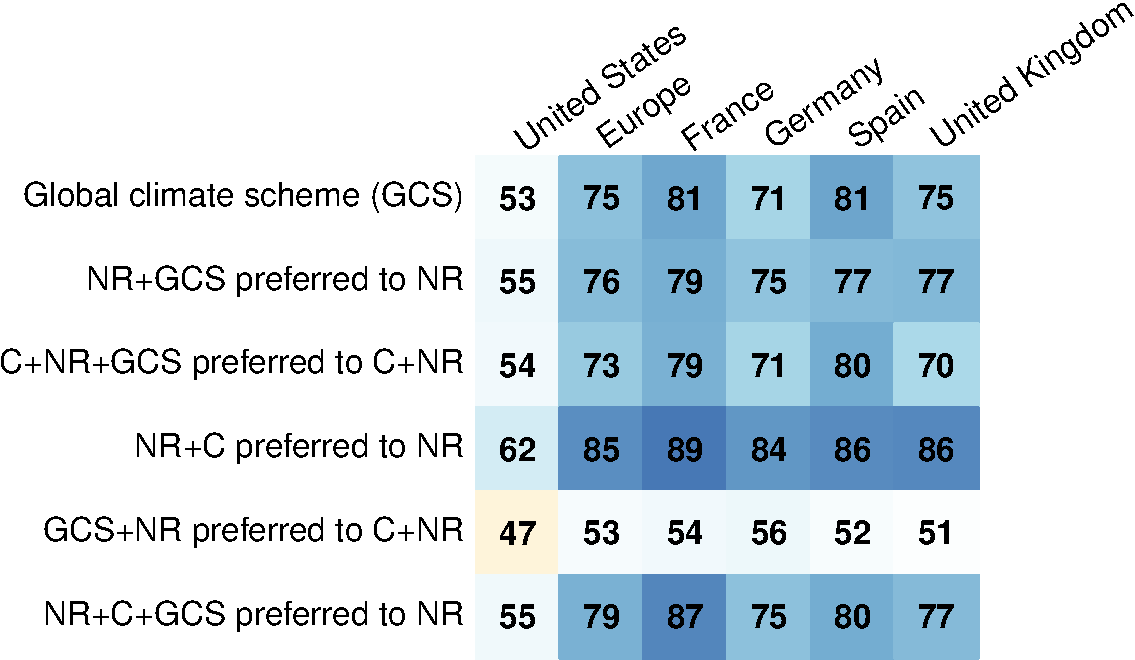
\includegraphics[width=.8\textwidth]{../figures/country_comparison/conjoint_ab_all_positive.pdf}} 
\end{figure}

% \begin{figure}[h!] % already in text
%     \caption{[Asked only to non-Republicans] Conjoint analysis n°4: random programs at the Democratic primary. (Question \ref{q:conjoint_r})}\label{fig:ca_r}
%     \makebox[\textwidth][c]{\includegraphics[width=\textwidth]{../figures/country_comparison/ca_r.png}} 
% \end{figure}

% \begin{figure}[h!]
%     \caption[Influence of the GCS on preferred platform]{Influence of the GCS on preferred platform:\\ Preference for a random platform A that contains the Global Climate Scheme rather than a platform B that does not (in percent). (Question \ref{q:conjoint_d}; in the U.S., asked only to non-Republicans.)}\label{fig:conjoint_left_ag_b}
%     \makebox[\textwidth][c]{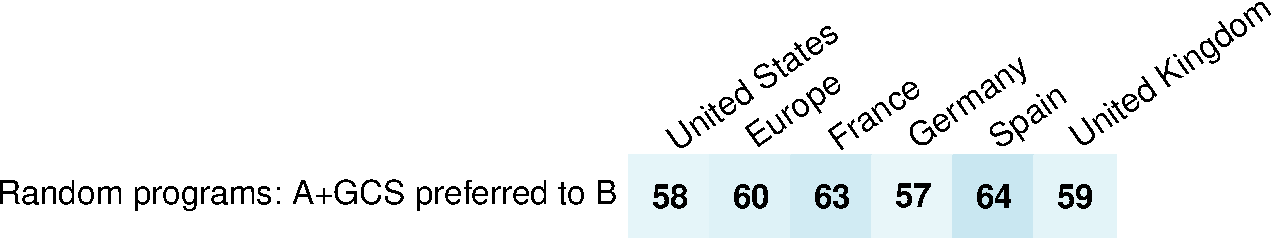
\includegraphics[width=\textwidth]{../figures/country_comparison/conjoint_left_ag_b_binary_positive.pdf}} 
% \end{figure}

\begin{figure}[h!]
    \caption[Perceptions of the GCS]{Perceptions of the GCS. Elements seen as important for supporting the GCS in a 4-Likert scale (in percent). (Question \ref{q:gcs_important})}\label{fig:gcs_important}
    \makebox[\textwidth][c]{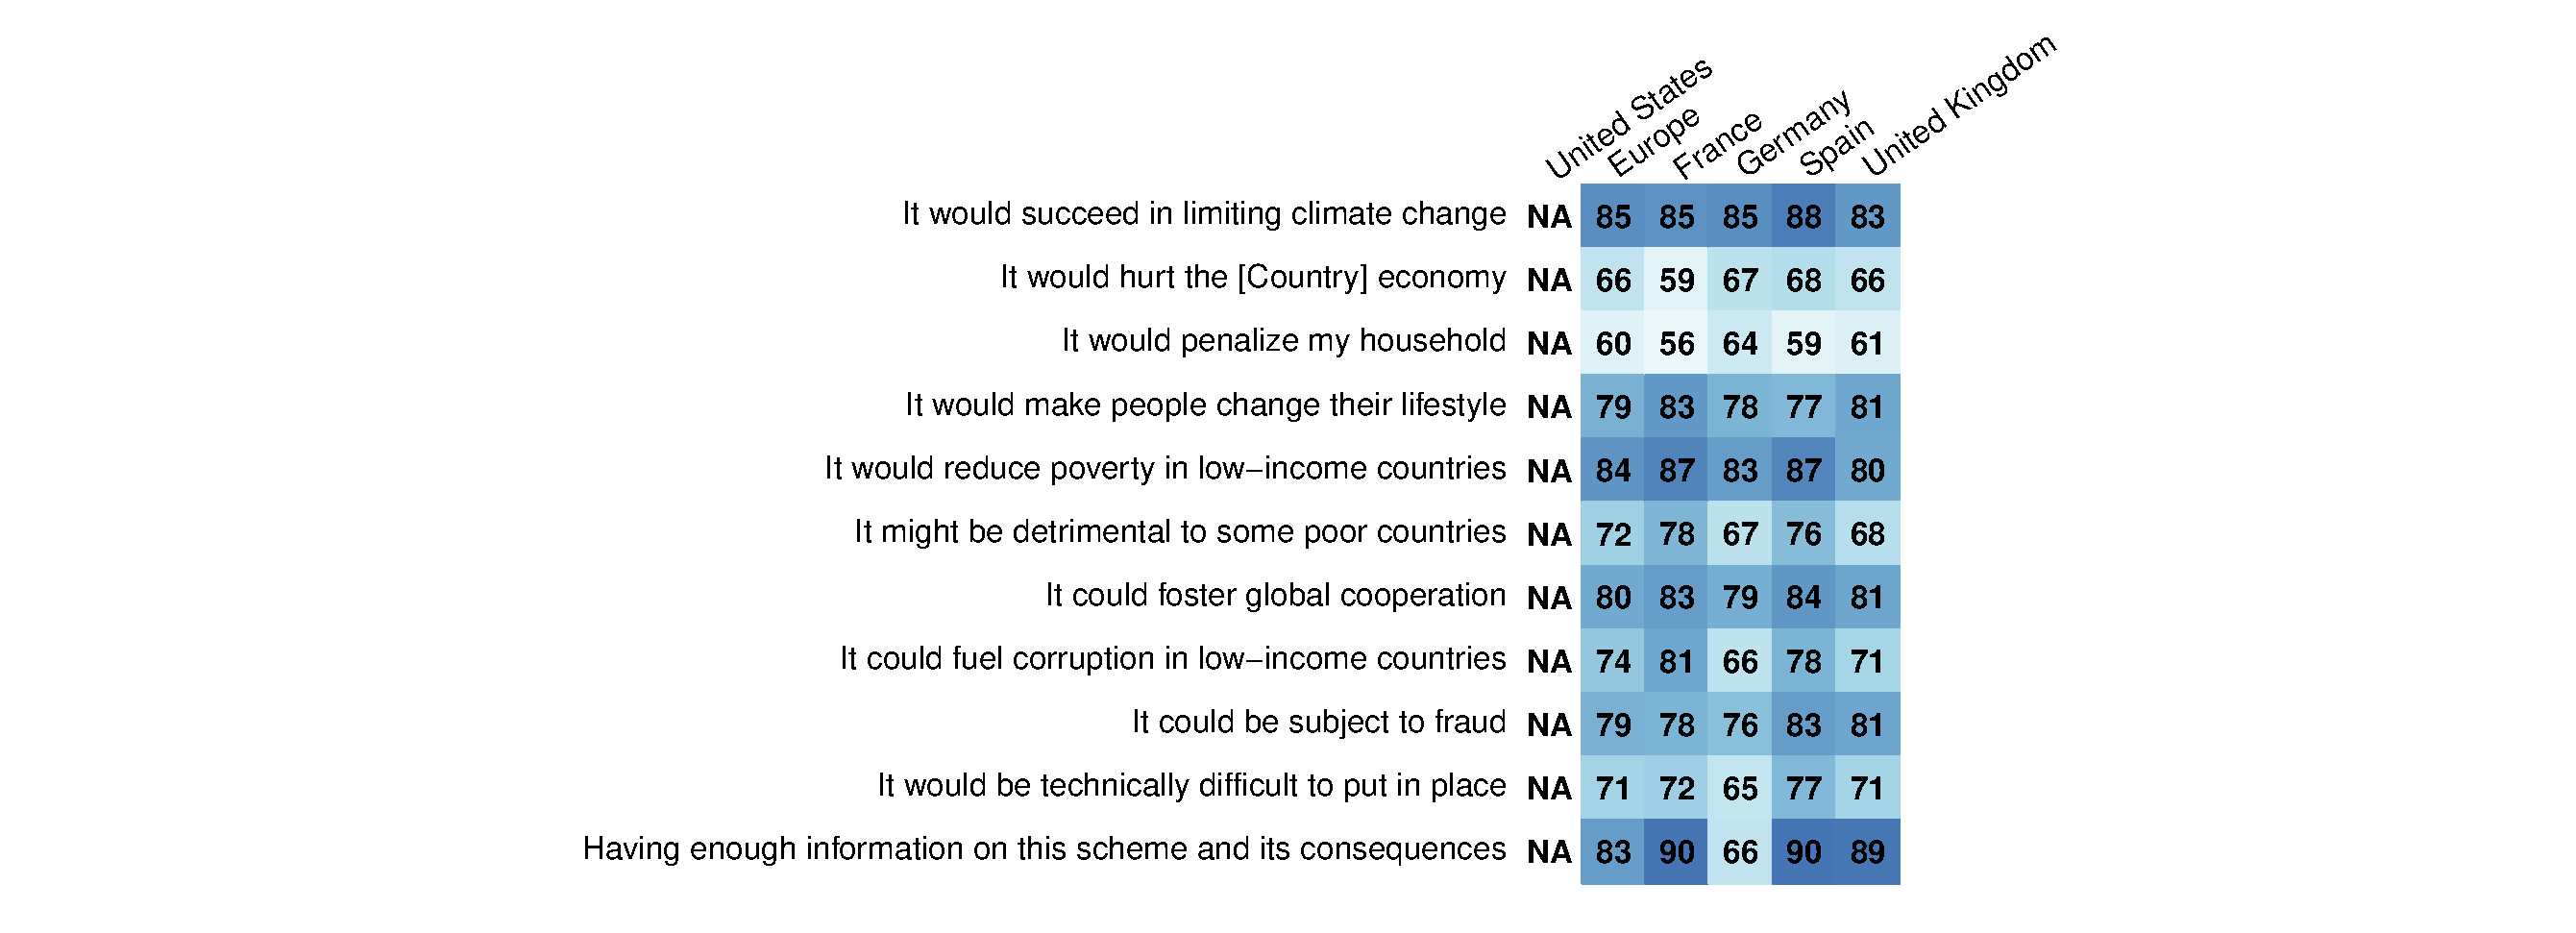
\includegraphics[width=\textwidth]{../figures/country_comparison/gcs_important_positive.pdf}} 
\end{figure}

\begin{figure}[h!]
    \caption[Classification of open-ended field on the GCS]{Perceptions of the GCS. Elements found in the open-ended field on the GCS (manually recoded, in percent). (Question \ref{q:gcs_field})}\label{fig:gcs_field}
    \makebox[\textwidth][c]{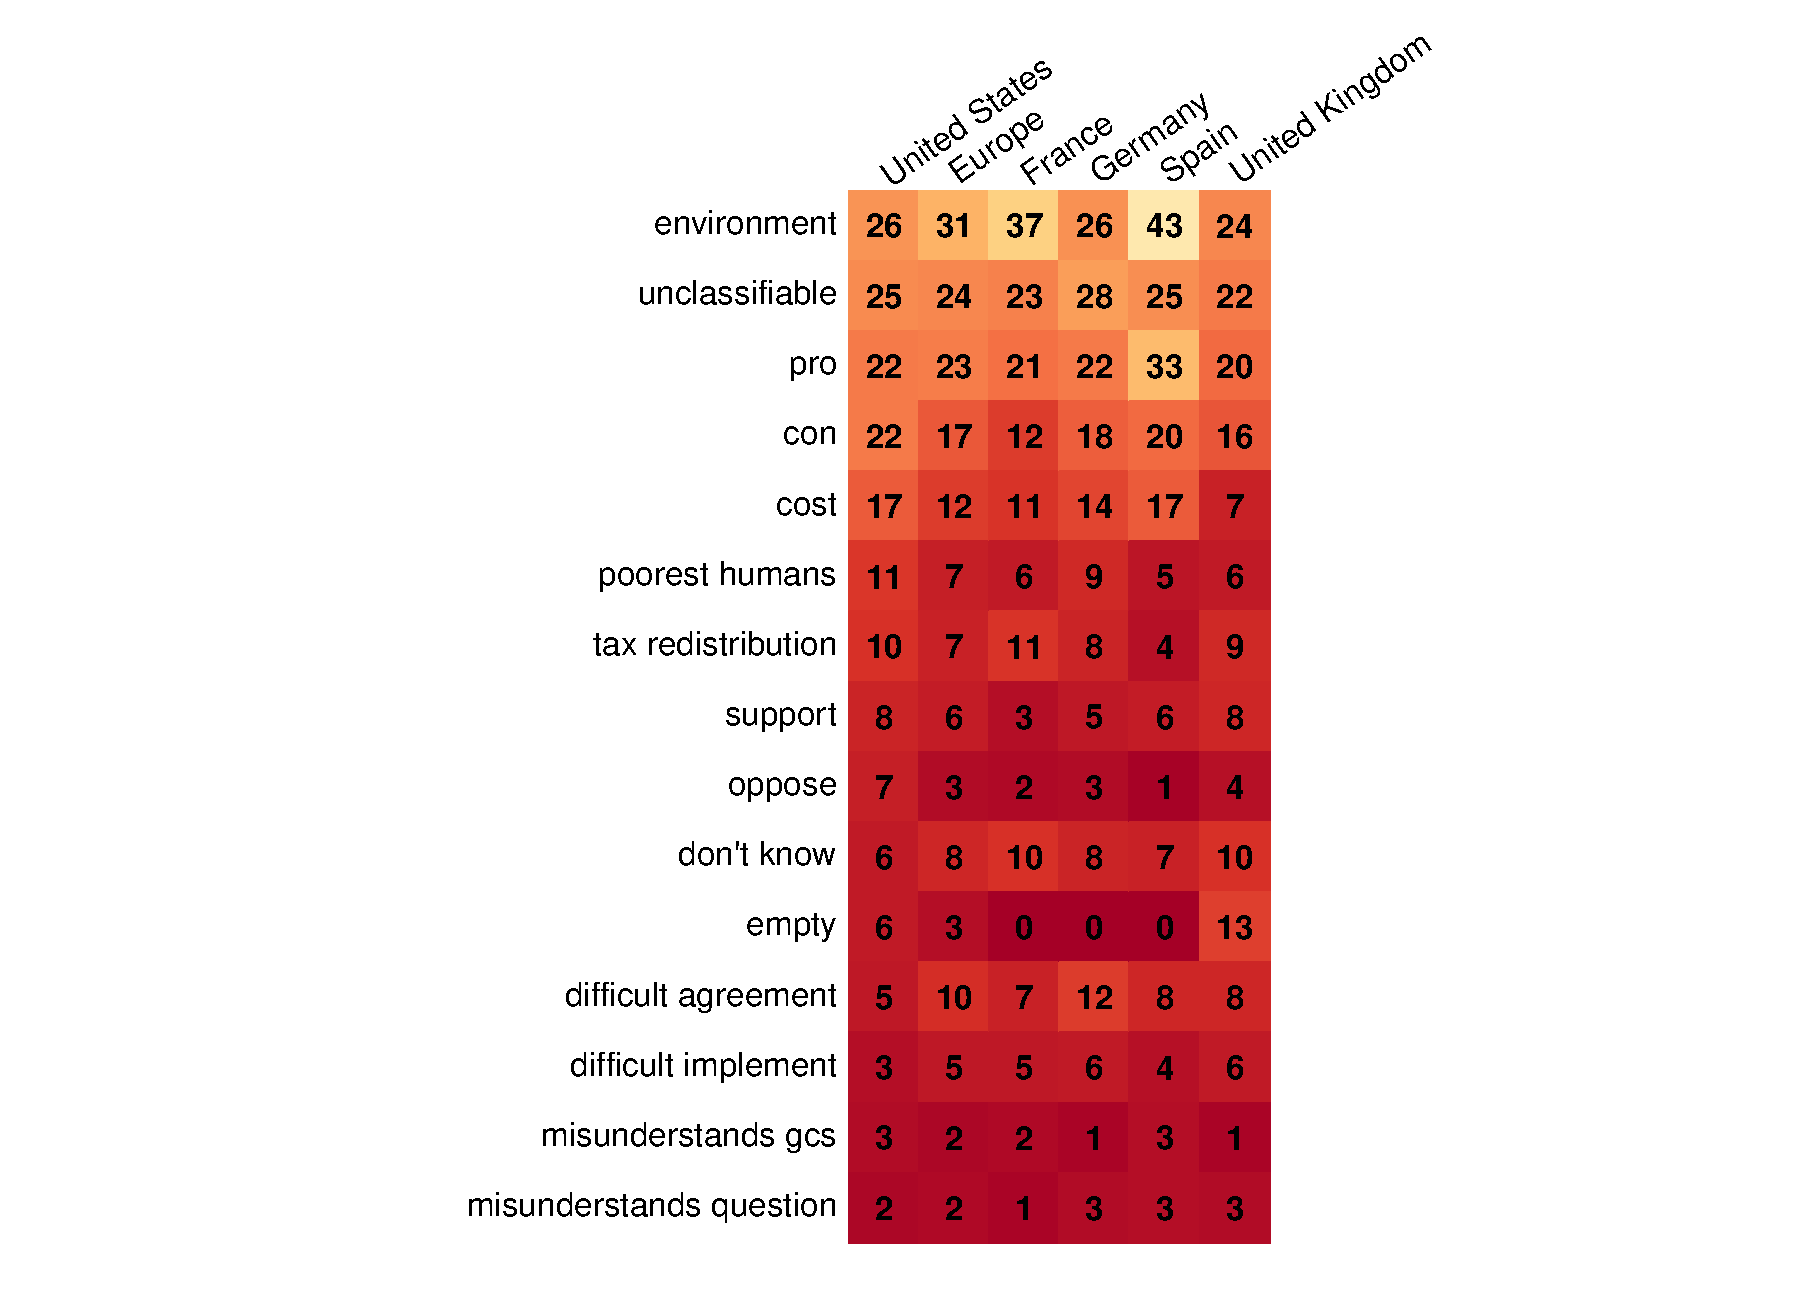
\includegraphics[width=.75\textwidth]{../figures/country_comparison/gcs_field_positive.pdf}} 
\end{figure}

\begin{figure}[h!]
    \caption[Topics of open-ended field on the GCS]{Perceptions of the GCS. Keywords found in the open-ended field on the GCS (automatic search ignoring case, in percent). (Question \ref{q:gcs_field})}\label{fig:gcs_field_contains}
    \makebox[\textwidth][c]{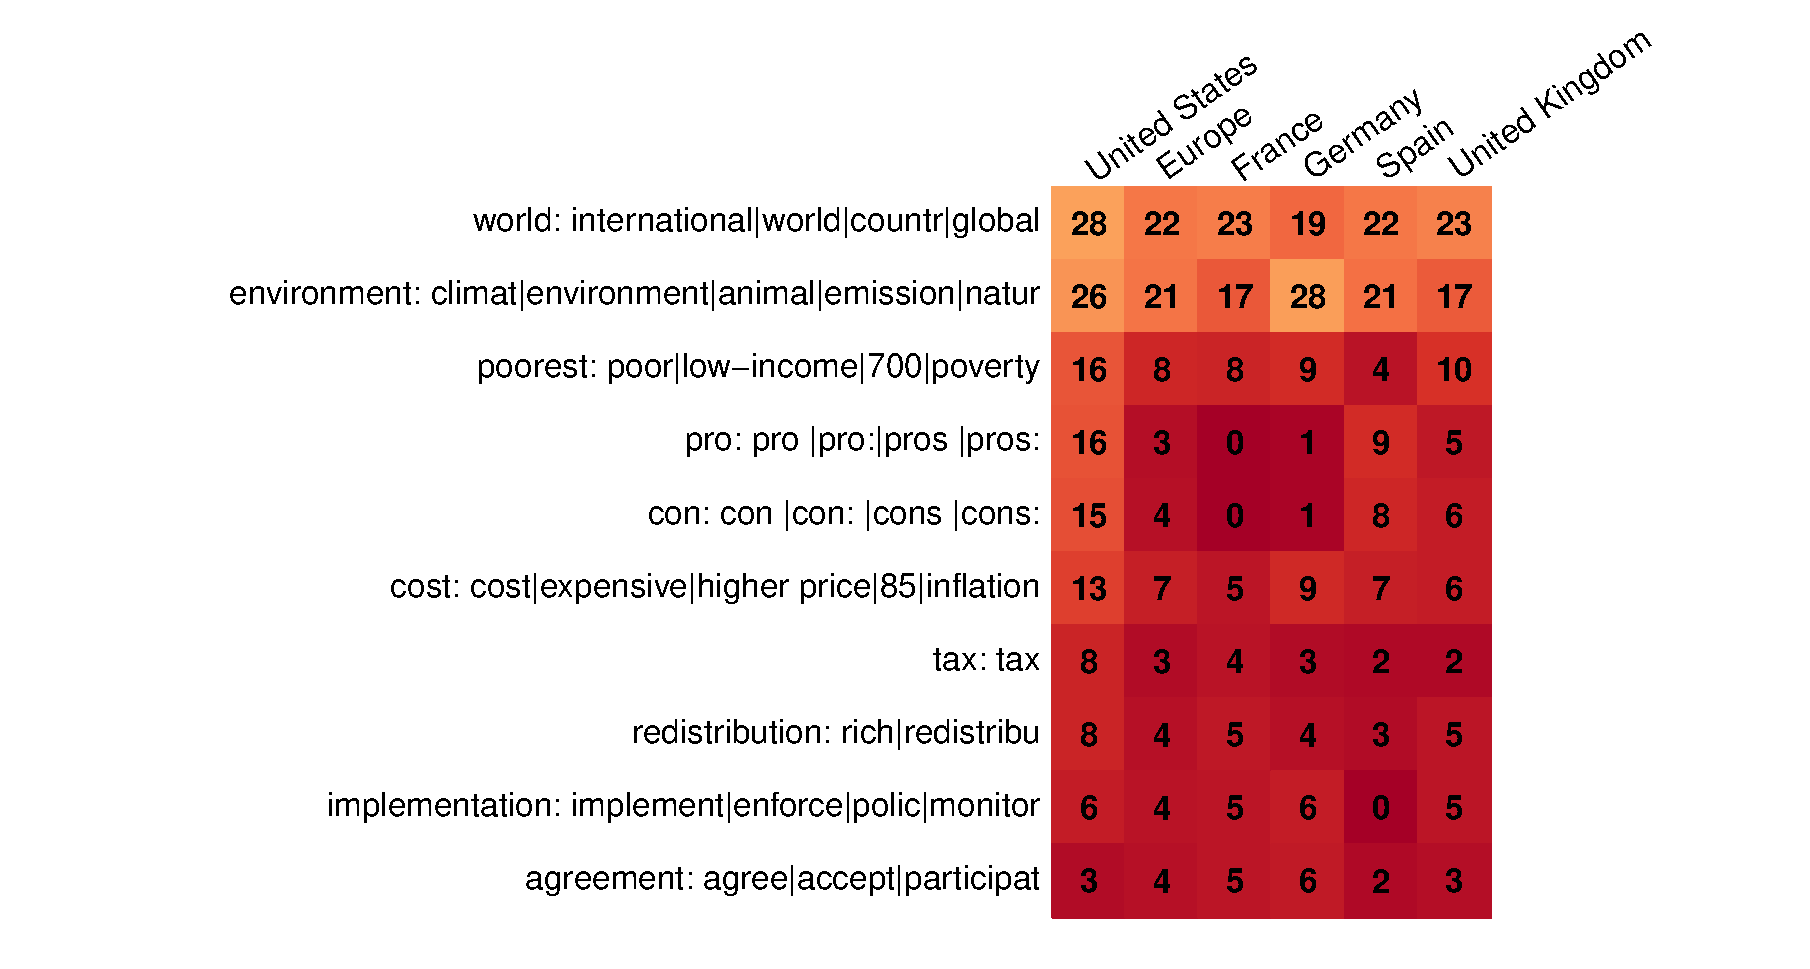
\includegraphics[width=\textwidth]{../figures/country_comparison/gcs_field_contains_positive.pdf}} 
\end{figure}

\begin{table}[h]\label{tab:branch_gcs}
    \caption[Campaign and bandwagon effects on the support for the GCS.]{Effects on the support for the GCS of a question on its pros and cons and on information about the actual support, in the U.S. (See Section \ref{subsec:questionnaire_perceptions} in the US2 Questionnaire)} 
    \makebox[\textwidth][c]{
        
\begin{tabular}{@{\extracolsep{5pt}}lcccc} 
\\[-1.8ex]\hline 
\hline \\[-1.8ex] 
 & \multicolumn{4}{c}{Support} \\ 
\cline{2-5} 
\\[-1.8ex] & \multicolumn{2}{c}{Global Climate Scheme} & \multicolumn{2}{c}{National Redistribution} \\ 
\\[-1.8ex] & (1) & (2) & (3) & (4)\\ 
\hline \\[-1.8ex] 
Control group mean & 0.557 & 0.557 & 0.569 & 0.569  \\ \hline \\[-1.8ex]
 Treatment: Open\mbox{-}ended field on GCS pros \& cons & $-$0.073$^{**}$ & $-$0.071$^{**}$ & $-$0.035 & $-$0.030 \\ 
  & (0.035) & (0.031) & (0.035) & (0.032) \\ 
  Treatment: Closed questions on GCS pros \& cons & $-$0.109$^{***}$ & $-$0.096$^{***}$ & $-$0.065$^{*}$ & $-$0.062$^{**}$ \\ 
  & (0.034) & (0.031) & (0.034) & (0.031) \\ 
  Treatment: Info on actual support for GCS and NR & $-$0.021 & $-$0.015 & 0.048 & 0.056$^{*}$ \\ 
  & (0.034) & (0.031) & (0.033) & (0.031) \\ 
 \hline \\[-1.8ex] 
Includes controls &  & \checkmark &  & \checkmark \\

Observations & 2,000 & 1,995 & 2,000 & 1,995 \\ 
R$^{2}$ & 0.007 & 0.170 & 0.007 & 0.154 \\ 
\hline 
\hline \\[-1.8ex] 
\end{tabular} 
    }
    {\footnotesize %\textit{Note}: 
    }
\end{table}

\begin{figure}[h!]
    \caption[Donation to Africa vs. own country]{Donation in case of lottery win, depending on the recipient's (randomly drawn) nationality (mean). (Question \ref{q:donation})}\label{fig:donation}
    \makebox[\textwidth][c]{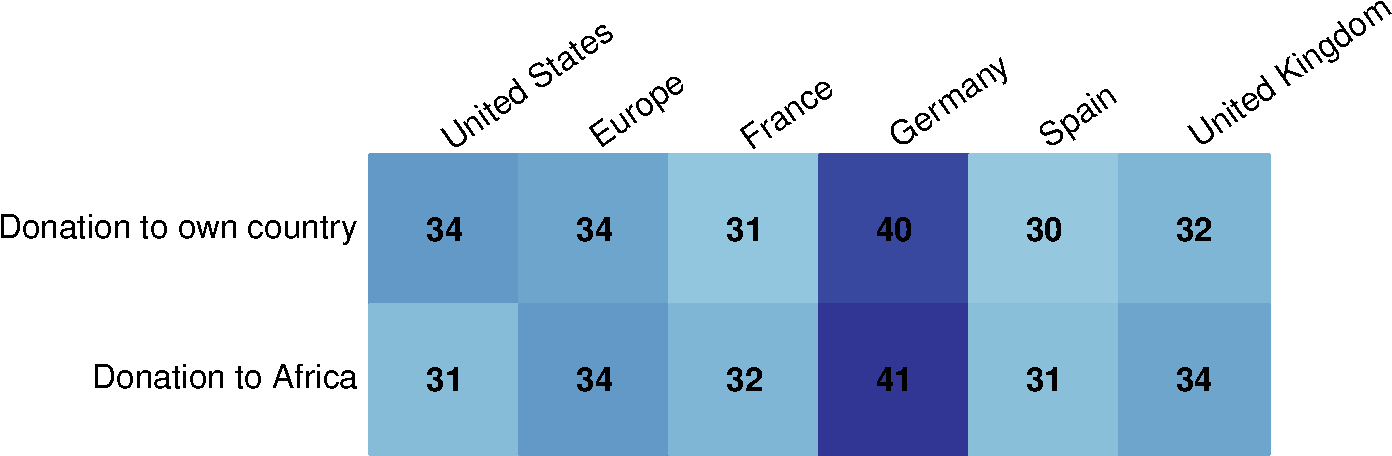
\includegraphics[width=.8\textwidth]{../figures/country_comparison/donation_mean.pdf}} 
\end{figure}

\begin{figure}[h!]
    \caption[Support for a global wealth tax]{Support for a global wealth tax. \\
    ``Do you support or oppose a tax on millionaires of all countries to finance low-
    income countries? \\
    Such tax would finance infrastructure and public services such as access to drinking water, healthcare, and education.'' (Question \ref{q:global_tax})}\label{fig:global_tax}
    \makebox[\textwidth][c]{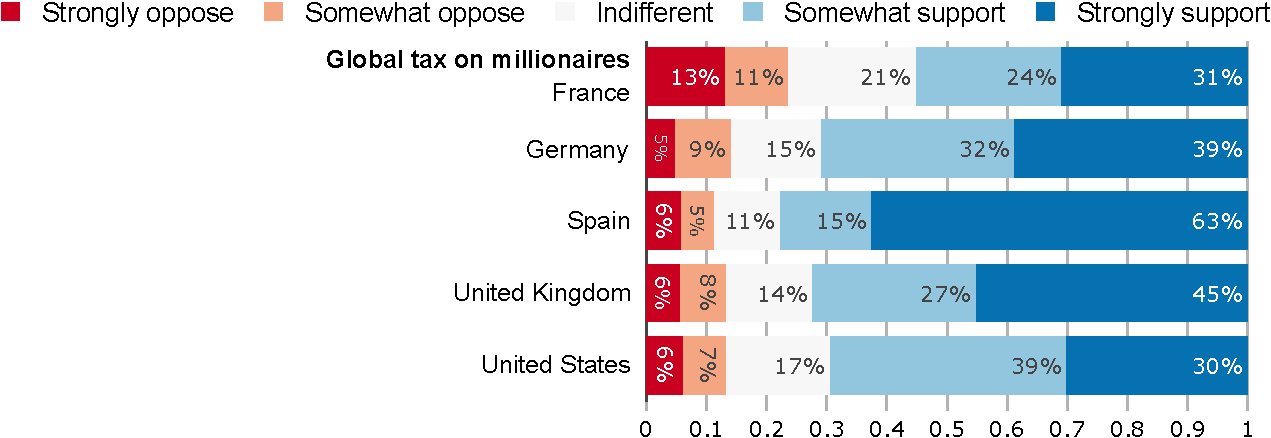
\includegraphics[width=\textwidth]{../figures/country_comparison/global_tax_support.pdf}} 
\end{figure}

\begin{figure}[h!]
    \caption[Support for a national wealth tax]{Support for a national wealth tax financing public services like healthcare, education, and social housing. (Question \ref{q:national_tax})}\label{fig:national_tax}
    \makebox[\textwidth][c]{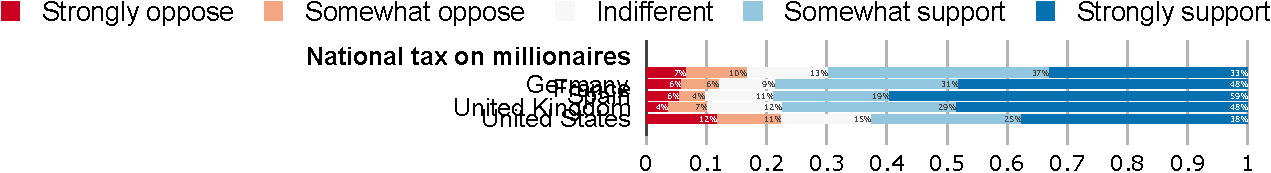
\includegraphics[width=\textwidth]{../figures/country_comparison/national_tax_support.pdf}} 
\end{figure}

\begin{figure}[h!]
    \caption[Preferred share of global tax for low-income countries]{Preferred share of global wealth tax revenues that should be pooled to finance low-income countries. (Question \ref{q:global_tax_global_share})}\label{fig:global_tax_global_share}
    \makebox[\textwidth][c]{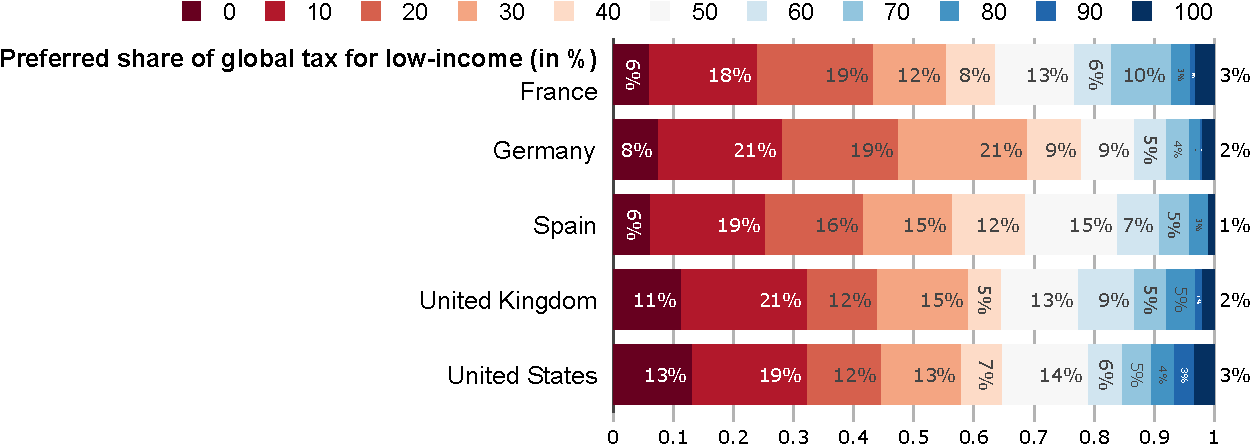
\includegraphics[width=\textwidth]{../figures/country_comparison/global_tax_global_share.pdf}} 
\end{figure}

\begin{figure}[h!]
    \caption[Support for sharing half of global tax revenues with low-income countries]{Support for sharing half of global tax revenues with low-income countries, rather that each country retaining all the revenues it collects (in percent). (Question \ref{q:global_tax_sharing})}\label{fig:global_tax_sharing}
    \makebox[\textwidth][c]{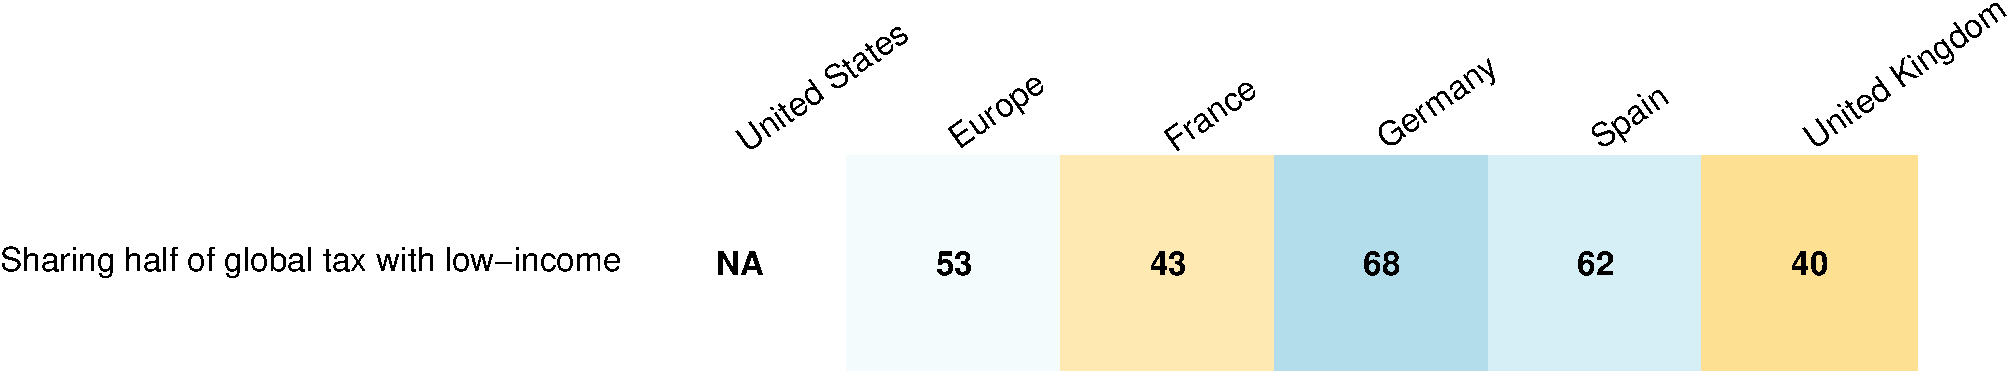
\includegraphics[width=\textwidth]{../figures/country_comparison/global_tax_sharing_positive.pdf}} 
\end{figure}

\begin{figure}[h!]
    \caption[Perceived foreign aid]{Perceived foreign aid. ``From your best guess, what percentage of [own country] government spending is allocated to foreign aid (that is, to reduce poverty in low-income countries)?'' (Question \ref{q:foreign_aid_belief})}\label{fig:foreign_aid_belief}
    \makebox[\textwidth][c]{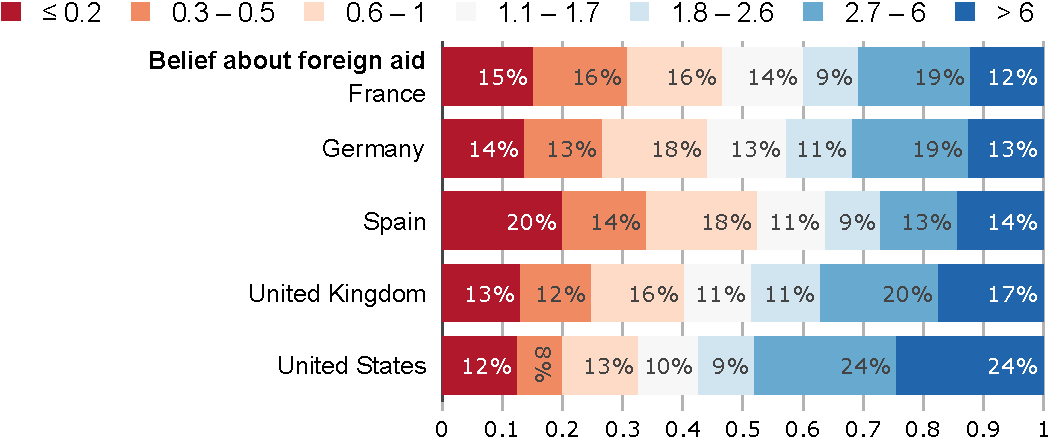
\includegraphics[width=\textwidth]{../figures/country_comparison/foreign_aid_belief_agg.pdf}} 
\end{figure}

\begin{figure}[h!]
    \caption[Preferred foreign aid (without info on actual amount)]{Preferred foreign aid (without info on actual amount). \\ ``If you could choose the government spending, what percentage would you allocate
    to foreign aid?'' (Question \ref{q:foreign_aid_preferred})}\label{fig:foreign_aid_preferred_no_info}
    \makebox[\textwidth][c]{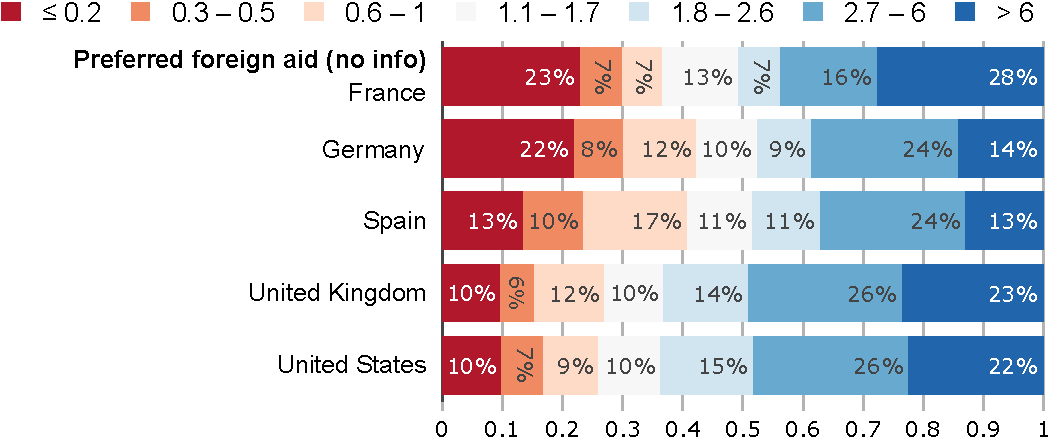
\includegraphics[width=\textwidth]{../figures/country_comparison/foreign_aid_preferred_no_info_agg.pdf}} 
\end{figure}

\begin{figure}[h!]
    \caption[Preferred foreign aid (after info on actual amount)]{Preferred foreign aid (after info on actual amount). \\ ``Actually,
    [US1: 0.4\%; FR: 0.8\%; DE: 1.3\%; ES: 0.5\%; UK: 1.7\%] of [own country] government spending is allocated to foreign aid. \\
    If you could choose the government spending, what percentage would you allocate
    to foreign aid?'' (Question \ref{q:foreign_aid_preferred})}\label{fig:foreign_aid_preferred_info}
    \makebox[\textwidth][c]{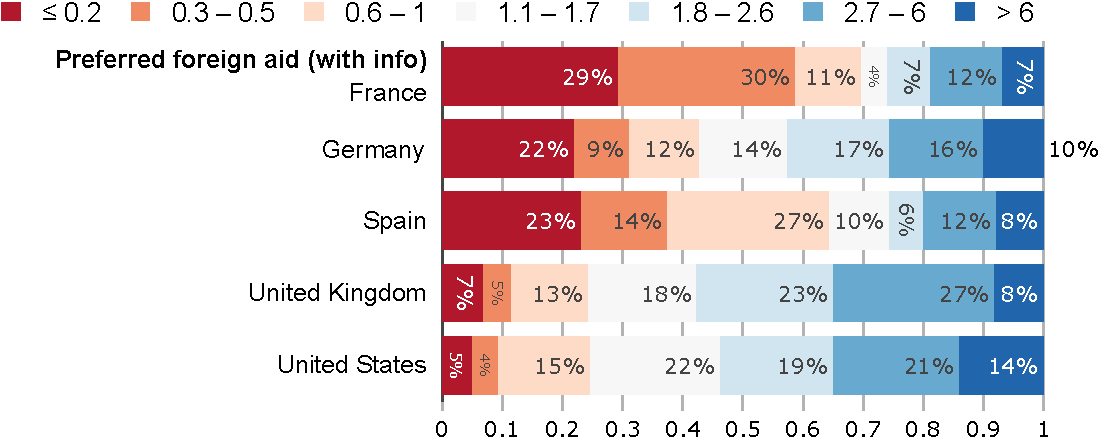
\includegraphics[width=\textwidth]{../figures/country_comparison/foreign_aid_preferred_info_agg.pdf}} 
\end{figure}

\begin{figure}[h!]
    \caption[Preferences for funding increased foreign aid]{Preferences for funding increased foreign aid. [Asked iff preferred foreign aid is strictly greater than [Info: actual; No info: perceived] foreign aid] \\ ``How would you like to finance such increase in foreign aid? (Multiple answers possible)'' (in percent) (Question \ref{q:foreign_aid_raise_how})}\label{fig:foreign_aid_raise_how}
    \makebox[\textwidth][c]{\includegraphics[width=.75\textwidth]{../figures/country_comparison/foreign_aid_raise_positive.pdf}} 
\end{figure}

\begin{figure}[h!]
    \caption[Preferences of spending following reduced foreign aid]{Preferences of spending following reduced foreign aid. [Asked iff preferred foreign aid is strictly lower than [Info: actual; No info: perceived] foreign aid] \\ ``How would you like to use the freed budget? (Multiple answers possible)'' (in percent) (Question \ref{q:foreign_aid_reduce_how})}\label{fig:foreign_aid_reduce_how}
    \makebox[\textwidth][c]{\includegraphics[width=.75\textwidth]{../figures/country_comparison/foreign_aid_reduce_positive.pdf}} 
\end{figure}

% \begin{figure}[h!]
%     \caption[Attitudes on the evolution of foreign aid]{Attitudes regarding the evolution of [own country] foreign aid. (Question \ref{q:foreign_aid_raise_support})}\label{fig:foreign_aid_raise_support}
%     \makebox[\textwidth][c]{\includegraphics[width=\textwidth]{../figures/country_comparison/foreign_aid_raise_support.pdf}} 
% \end{figure}

% \begin{figure}[h!]
%     \caption[Conditions at which foreign aid should be increased]{Conditions at which foreign aid should be increased (in percent). [Asked to those who wish an increase of foreign aid at some conditions.] (Question \ref{q:foreign_aid_condition})}\label{fig:foreign_aid_condition}
%     \makebox[\textwidth][c]{\includegraphics[width=\textwidth]{../figures/country_comparison/foreign_aid_condition_positive.pdf}} 
% \end{figure}

% \begin{figure}[h!]
%     \caption[Reasons why foreign aid should not be increased]{Reasons why foreign aid should not be increased (in percent). [Asked to those who wish a decrease or stability of foreign aid.] (Question \ref{q:foreign_aid_no})}\label{fig:foreign_aid_no}
%     \makebox[\textwidth][c]{\includegraphics[width=\textwidth]{../figures/country_comparison/foreign_aid_no_positive.pdf}} 
% \end{figure}

% \begin{figure}[h!]
%     \caption[Willingness to sign a real-stake petition]{Willingness to sign real-stake petition for the Global Climate Scheme or National Redistribution. (Question \ref{q:petition})}\label{fig:petition}
%     \makebox[\textwidth][c]{\includegraphics[width=.8\textwidth]{../figures/country_comparison/petition_only_positive.pdf}} 
% \end{figure}

\begin{figure}[h!]
    \caption[Willingness to sign a real-stake petition]{Willingness to sign real-stake petition for the Global Climate Scheme or National Redistribution, compared to stated support in corresponding subsamples (e.g. support for the GCS in the branch where the petition was about the GCS). (Question \ref{q:petition})}\label{fig:petition}
    \makebox[\textwidth][c]{\includegraphics[width=.8\textwidth]{../figures/country_comparison/petition_comparable_positive.pdf}} 
\end{figure}

\begin{figure}[h!] % TODO? More details?
    \caption[Absolute support for various global policies]{Absolute support for various global policies (Percent of (\textit{somewhat} or \textit{strong}) support). (Questions \ref{q:climate_policies} and \ref{q:other_policies}. See Figure \ref{fig:support} for the relative support.)}\label{fig:support_likert_positive}
    \makebox[\textwidth][c]{\includegraphics[width=\textwidth]{../figures/country_comparison/support_likert_positive.pdf}} 
\end{figure}

% \begin{figure}[h!]
%     \caption{label}\label{fig:climate_policies}
%     \makebox[\textwidth][c]{\includegraphics[width=\textwidth]{../figures/country_comparison/climate_policies.pdf}} 
% \end{figure}

% \begin{figure}[h!]
%     \caption{label}\label{fig:global_policies}
%     \makebox[\textwidth][c]{\includegraphics[width=\textwidth]{../figures/country_comparison/global_policies.pdf}} 
% \end{figure}

\begin{figure}[h!]
    \caption[Preferred approach for international climate negotiations]{Preferred approach of diplomats at international climate negotiations. \\ In international climate negotiations, would you prefer [U.S.] diplomats to defend [own country] interests or global justice? (Question \ref{q:negotiation})}\label{fig:negotiation}
    \makebox[\textwidth][c]{\includegraphics[width=\textwidth]{../figures/country_comparison/negotiation.pdf}} 
\end{figure}

\begin{figure}[h!]
    \caption[Importance of selected issues]{Percent of selected issues viewed as important.\\ ``To what extent do you think the following issues are a problem?'' (Question \ref{q:problem})}\label{fig:problem}
    \makebox[\textwidth][c]{\includegraphics[width=.75\textwidth]{../figures/country_comparison/problem_positive.pdf}} 
\end{figure}

\begin{figure}[h!]
    \caption[Group defended when voting]{Group defended when voting. \\ ``What group do you defend when you vote?'' (Question \ref{q:group_defended})}\label{fig:group_defended}
    \makebox[\textwidth][c]{\includegraphics[width=\textwidth]{../figures/country_comparison/group_defended_agg2.pdf}} 
\end{figure}

% \begin{figure}[h!]
%     \caption{label}\label{fig:group_defended}
%     \makebox[\textwidth][c]{\includegraphics[width=\textwidth]{../figures/country_comparison/group_defended.pdf}} 
% \end{figure}

\begin{figure}[h!] 
    \caption[Mean prioritization of policies]{Mean prioritization of policies. \\Mean number of points allocated policies to express intensity of support (among six policies chosen at random). Blue color means that the policy has been awarded more points than the average policy. (Question \ref{q:points})}\label{fig:points}
    \makebox[\textwidth][c]{\includegraphics[width=\textwidth]{../figures/country_comparison/points_mean.pdf}} 
\end{figure}

\begin{figure}[h!] 
    \caption[Positive prioritization of policies]{Positive prioritization of policies. \\ Percent of people allocating a positive number of points to policies, expressing their support (among six policies chosen at random). (Question \ref{q:points})}\label{fig:points_positive}
    \makebox[\textwidth][c]{\includegraphics[width=\textwidth]{../figures/country_comparison/points_positive.pdf}} 
\end{figure}

\begin{figure}[h!]
    \caption[Charity donation]{Charity donation. \\ ``How much did you give to charities in 2022?'' (Question \ref{q:donation_charities})}\label{fig:donation_charities}
    \makebox[\textwidth][c]{\includegraphics[width=.8\textwidth]{../figures/country_comparison/donation_charities.pdf}} 
\end{figure}

\begin{figure}[h!] 
    \caption[Interest in politics]{Interest in politics. \\ ``To what extent are you interested in politics?'' (Question \ref{q:interested_politics})}\label{fig:interested_politics}
    \makebox[\textwidth][c]{\includegraphics[width=.8\textwidth]{../figures/country_comparison/interested_politics.pdf}} 
\end{figure}

\begin{figure}[h!] 
    \caption[Desired involvement of government]{Desired involvement of government (from 1 to 5). (Question \ref{q:involvement_govt})}\label{fig:involvement_govt}
    \makebox[\textwidth][c]{\includegraphics[width=.9\textwidth]{../figures/country_comparison/involvement_govt.pdf}} 
\end{figure}

\begin{figure}[h!] 
    \caption[Political leaning]{Political leaning on economics (from 1: Left to 5: Right). (Question \ref{q:left_right})}\label{fig:left_right}
    \makebox[\textwidth][c]{\includegraphics[width=.8\textwidth]{../figures/country_comparison/left_right.pdf}} 
\end{figure}

\begin{figure}[h!] 
    \caption[Voted in last election]{Voted in last election. (Question \ref{q:vote_participation})}\label{fig:vote_participation}
    \makebox[\textwidth][c]{\includegraphics[width=.8\textwidth]{../figures/country_comparison/vote_participation.pdf}} 
\end{figure}

\begin{figure}[h!] 
    \caption[Vote in last election]{Vote in last election (aggregated). \textit{PNR} includes people who did not vote or prefer not to answer. (Question \ref{q:vote})}\label{fig:vote}
    \makebox[\textwidth][c]{\includegraphics[width=.75\textwidth]{../figures/country_comparison/vote.pdf}} 
\end{figure}

\begin{figure}[h!] 
    \caption[Perception that survey was biased]{Perception that survey was biased. \\ ``Do you feel that this survey was politically biased?'' (Question \ref{q:survey_biased})}\label{fig:survey_biased}
    \makebox[\textwidth][c]{\includegraphics[width=.7\textwidth]{../figures/country_comparison/survey_biased.pdf}} 
\end{figure}

% \begin{columns}
% \begin{column}{.5\textwidth}
% \begin{multicols}{2}
    \begin{figure}[h!]
        \caption[Classification of open-ended field on extreme poverty]{Opinion on the fight against extreme poverty. \\ ``According to you, what should high-income countries do to fight extreme poverty in low-income countries?'' (Question \ref{q:poverty_field})}\label{fig:poverty_field}
    \begin{subfigure}{.34\textwidth}
        \caption{Elements found in the open-ended field on the question (manually recoded, in percent)}.
        \includegraphics[width=\textwidth]{../figures/country_comparison/poverty_field_positive.pdf}        
    \end{subfigure}
    \hspace{.02\textwidth}
    \begin{subfigure}{.64\textwidth}
        \caption{Keywords found in the open-ended field on the GCS (automatic search ignoring case, in percent).}
        \includegraphics[width=\textwidth]{../figures/country_comparison/poverty_field_contains_positive.pdf}    
    \end{subfigure}
    \end{figure}
% \end{column}
% \begin{column}{.5\textwidth}
    % \begin{figure}[h!]
    %     \caption[Topics of open-ended field on extreme poverty]{Opinion on the fight against extreme poverty. \\ ``According to you, what should high-income countries do to fight extreme poverty in low-income countries?'' \\ Keywords found in the open-ended field on the GCS (automatic search ignoring case, in percent). (Question \ref{q:poverty_field})}\label{fig:poverty_field_contains}
    %     \makebox[\textwidth][c]{\includegraphics[width=\columnwidth]{../figures/country_comparison/poverty_field_contains_positive.pdf}} 
    % \end{figure}
% \end{multicols}
% \end{column}
% \end{columns}


% \begin{figure}[h!] 
%     \caption[Interested to be interviewed]{Interested to be interviewed by a researcher for 30 min through videoconference. (Question \ref{q:interview})}\label{fig:interview}
%     \makebox[\textwidth][c]{\includegraphics[width=\textwidth]{../figures/country_comparison/interview.pdf}} 
% \end{figure}    

% \begin{figure}[h!]
%     \caption{label}\label{fig:share_policies_supported}
%     \makebox[\textwidth][c]{\includegraphics[width=\textwidth]{../figures/country_comparison/share_policies_supported.pdf}} 
% \end{figure} % TODO? uncomment?

% \begin{figure}[h!]
%     \caption{label}\label{fig:vars}
%     \makebox[\textwidth][c]{\includegraphics[width=\textwidth]{../figures/country_comparison/vars.pdf}} 
% \end{figure}

% In Denmark, France and the U.S., the questions with an asterisk were asked differently, asking ``To achieve a given reduction of greenhouse gas emissions globally, costly investments are needed. Ideally, how should countries bear the costs of fighting climate change?''. Instead of the equal right per capita, the item was ``Countries should pay in proportion to their current emissions'', historical responsibilities was worded as ``Countries should pay in proportion to their past emissions (from 1990 onwards)'', then there was an item ``The richest countries should pay it all'', and compensating vulnerable countries was worded as ``The richest countries should pay even more, to help vulnerable countries face adverse consequences: vulnerable countries would then receive money instead of paying''.

\clearpage 
\section{Questionnaire of the global survey (section on global policies)}\label{app:questionnaire_oecd}
%\subsection*{International burden-sharing}
\renewcommand{\theenumi}{\Alph{enumi}}
\begin{enumerate} \item \label{q:scale} At which level(s) do you think public policies to tackle climate change need to be put in place? (Multiple answers are possible) [\textit{Figures \ref{fig:oecd} and \ref{fig:oecd_absolute}}]
\\ \textit{Global; [Federal / European / ...]; [State / National]; Local}
\item Do you agree or disagree with the following statement: ``[country] should take measures to fight climate change.''% TODO! figure
	\\ \textit{Strongly disagree; Somewhat disagree; Neither agree nor disagree; Somewhat agree; Strongly agree}
\item How should [country] climate policies depend on what other countries do?% TODO! figure
 \begin{itemize}
\item If other countries do more, [country] should do...
\item If other countries do less, [country] should do...
\end{itemize}
\textit{Much less; Less; About the same; More; Much more}
\item ~[In all countries but the U.S., Denmark and France]  All countries have signed the Paris agreement that aims to contain global warming ``well below +2 \textdegree{}C\''. To limit global warming to this level, there is a maximum amount of greenhouse gases we can emit globally, called the carbon budget. Each country could aim to emit less than a share of the carbon budget. To respect the global carbon budget, countries that emit more than their national share would pay a fee to countries that emit less than their share. \\ 
Do you support such a policy? [\textit{Figures \ref{fig:oecd} and \ref{fig:oecd_absolute}}]
\\ \textit{Strongly oppose; Somewhat oppose; Neither support nor oppose; Somewhat support; Strongly support}
\item ~[In all countries but the U.S., Denmark and France] Suppose the above policy is in place. How should the carbon budget be divided among countries? [\textit{Figures \ref{fig:oecd} and \ref{fig:oecd_absolute}}]
\\ \textit{The emission share of a country should be proportional to its population, so that each human has an equal right to emit.; The emission share of a country should be proportional to its current emissions, so that those who already emit more have more rights to emit.; Countries that have emitted more over the past decades (from 1990 onwards) should receive a lower emission share, because they have already used some of their fair share.; Countries that will be hurt more by climate change should receive a higher emission share, to compensate them for the damages.}
\item \label{q:burden_sharing_asterisk} ~[In the U.S., Denmark, and France only] To achieve a given reduction of greenhouse gas emissions globally, costly investments are needed. % TODO! figure
Ideally, how should countries bear the costs of fighting climate change?
 \begin{itemize}
\item Countries should pay in proportion to their income
\item Countries should pay in proportion to their current emissions [Used as a substitute to the equal right per capita in Figure \ref{fig:oecd}]
\item Countries should pay in proportion to their past emissions (from 1990 onwards) [Used as a substitute to historical responsibilities in Figure \ref{fig:oecd}]
\item The richest countries should pay it all, so that the poorest countries do not have to pay anything
\item The richest countries should pay even more, to help vulnerable countries face adverse consequences: vulnerable countries would then receive money instead of paying [Used as a substitute to compensating vulnerable countries in Figures \ref{fig:oecd} and \ref{fig:oecd_absolute}]
\end{itemize} 
\textit{Strongly disagree; Somewhat disagree; Neither agree nor disagree; Somewhat agree; Strongly agree}
\item Do you support or oppose establishing a global democratic assembly whose role would be to draft international treaties against climate change? Each adult across the world would have one vote to elect members of the assembly. [\textit{Figures \ref{fig:oecd} and \ref{fig:oecd_absolute}}]
\\ \textit{Strongly oppose; Somewhat oppose; Neither support nor oppose; Somewhat support; Strongly support}
\item Imagine the following policy: a global tax on greenhouse gas emissions funding a global basic income. 
Such a policy would progressively raise the price of fossil fuels (for example, the price of gasoline would increase by [40 cents per gallon] in the first years). Higher prices would encourage people and companies to use less fossil fuels, reducing greenhouse gas emissions. Revenues from the tax would be used to finance a basic income of [\$30] per month to each human adult, thereby lifting the 700 million people who earn less than \$2/day out of extreme poverty. 
The average British person would lose a bit from this policy as they would face [\$130] per month in price increases, which is higher than the [\$30] they would receive.

Do you support or oppose such a policy?  [\textit{Figures \ref{fig:oecd} and \ref{fig:oecd_absolute}}]
\\ \textit{Strongly oppose; Somewhat oppose; Neither support nor oppose; Somewhat support; Strongly support}
\item \label{q:millionaire_tax} Do you support or oppose a tax on all millionaires around the world to finance low-income countries that comply with international standards regarding climate action? 
This would finance infrastructure and public services such as access to drinking water, healthcare, and education. [\textit{Figures \ref{fig:oecd} and \ref{fig:oecd_absolute}}]
\\ \textit{Strongly oppose; Somewhat oppose; Neither support nor oppose; Somewhat support; Strongly support}
\end{enumerate}

% \clearpage
% \section{Questionnaire of US1 %the first U.S. complementary 
% survey}\label{app:questionnaire_US1}

% \begin{figure}[h!]
%     \caption{US1 survey structure}\label{fig:flow_US1}
%     \makebox[\textwidth][c]{\includegraphics[width=\textwidth]{../questionnaire/survey_flow_US1.pdf}} 
% \end{figure}

\renewcommand{\theenumi}{\arabic{enumi}}
\clearpage
\section{Questionnaire of the complementary surveys}\label{app:questionnaire}
% /!\ Ctrl+H "\item ~[" / "\\ ["=> "\item ~[" / "\\ ~["
% TODO!? put in italic the "didascalies" in []
% TODO? give policies options here instead of referring to "this spreadsheet"
Below, we provide the generic questionnaire (based on the U.S. version), which roughly corresponds to the \textit{Eu} questionnaire as well as the combination of the \textit{US1} and \textit{US2} questionnaire. The main difference between Europe and the U.S. is that we split the \textit{US2} sample into four random branches to include some treatments before the Section \ref{subsec:questionnaire_GCS} on the GCS. Besides the control group, the treatments are: information regarding the support of Americans for the GCS and NR, an open-ended field, and a closed question on the pros and cons of the GCS. The pros and cons of the GCS are also asked in \textit{Eu} (likewise, either as an open-ended field or a question), but only in Section \ref{subsec:questionnaire_perceptions}, after the support. 

At each section or question, square brackets specify in which questionnaires it is present (\textit{US1}, \textit{US2} and/or \textit{Eu}) as well as country specificities. Figures \ref{fig:flow_Eu}-\ref{fig:flow_US2} display the structure of each questionnaire. Each treatment randomization is independent. Qualtrics and Word versions of the questionnaires in each language are available on our \href{https://github.com/bixiou/international_attitudes_toward_global_policies/tree/main/questionnaire}{public repository}, together with a spreadsheet that summarizes country specificities and our sources.

\begin{figure}[h!]
    \caption{\textit{Eu} survey structure}\label{fig:flow_Eu}
    \makebox[\textwidth][c]{\includegraphics[width=\textwidth]{../questionnaire/survey_flow_EU.pdf}} 
\end{figure}

\begin{figure}[h!]
    \caption{\textit{US1} survey structure}\label{fig:flow_US1}
    \makebox[\textwidth][c]{\includegraphics[width=\textwidth]{../questionnaire/survey_flow_US1.pdf}} 
\end{figure}

\begin{figure}[h!]
    \caption{\textit{US2} survey structure}\label{fig:flow_US2}
    \makebox[\textwidth][c]{\includegraphics[width=\textwidth]{../questionnaire/survey_flow_US2.pdf}} 
\end{figure}

\clearpage
\subsection*{[\textit{Eu}, \textit{US1}, \textit{US2}] Socio-demographic characteristics}
\begin{enumerate}
\item Welcome to this survey!\\
\\
This survey is \textbf{anonymous} and is conducted \textbf{for research} purposes on a representative sample of [1,000 British people].\\
 \\
It takes [\textit{US1}, \textit{US2}: 10 to 15 min; \textit{Eu}: around \textbf{20 min}] to complete.  \\
 \\
The survey contains lotteries and awards for those who get the correct answer to some understanding questions.\\
If you are attentive and lucky, \textbf{you can win up to }[\textit{US1}, \textit{Eu}: \textbf{\$350}; \textit{US2}: \textbf{\$150}] in points. (\href{https://uvafeb.eu.qualtrics.com/WRQualtricsControlPanel/File.php?F=F_cBZAXTgNktGZbee&download=1}{See terms and conditions}).    \\
Please answer every question carefully.  \\
 \\
\textbf{Do you agree to participate in the survey?}
\\ \textit{Yes; No}
\item What is your gender?
\\ \textit{Woman; Man; Other}
\item How old are you?
\\ \textit{Below 18; 18 to 20; 21 to 24; 25 to 29; 30 to 34; 35 to 39; 40 to 44; 45 to 49; 50 to 54; 55 to 59; 60 to 64; 65 to 69; 70 to 74; 75 to 79; 80 to 84; 85 to 89; 90 to 99; 100 or above}
\item ~[\textit{Eu}] In which country do you live?
\\ \textit{France; Germany; Spain; United Kingdom; Other}
\item What is your ZIP code? [UK: What is your Outcode (the left part of your postcode, e.g. if your postcode is N7 8H7, just enter N7)?]
\item \label{q:partner} Do you live with your partner (if you have one)?
\\ \textit{Yes; No}
\item How many people are in your household? The household includes: you, the members of your family who live with you, and your dependants. %This excludes flatmates.
\\ \textit{1; 2; 3; 4; 5 or more}
\item \label{q:children} [\textit{Eu}] How many children below 14 live with you?
\\ \textit{1; 2; 3; 4 or more}
\item ~[\textit{US1}, \textit{US2}] What race or ethnicity do you identify with? (Multiple answers are possible) 
\\ \textit{White; Black or African American; Hispanic; Asian; American Indian or Alaskan Native; Natice Hawaiian or Pacific Islander; Other: \{open field\}; Prefer not to say}
\item What is the [\textit{US1}, \textit{US2}: \textit{annual}; \textit{Eu}: \textit{monthly}] gross income of your household (before withholding tax)? This includes all income: wages, self-employment earnings, Social Security benefits, pensions, investment income, welfare payments, and income from other sources. % ~[quartiles thresholds are given for the U.S. ] 
\\ ~[\textit{US1}, \textit{US2}: Items based on household total income deciles and quartiles, namely: \textit{Less than \$20,000; between \$20,001 and \$35,000; between \$35,001 and \$42,000; between \$42,001 and \$50,000; between \$50,001 and \$65,000; between \$65,001 and \$82,000; between \$82,001 and \$103,000; between \$103,001 and \$130,000; between \$130,001 and \$145,000; between \$145,001 and \$165,000; between \$165,001 and \$250,000; More than \$250,000; I prefer not to answer}; \\ \textit{Eu}: custom thresholds, taking into account household composition Questions \ref{q:partner}-\ref{q:children}, and corresponding to the country's deciles and quartiles of standard of living, cf. the sheet ``Income'' in \href{https://github.com/bixiou/international_attitudes_toward_global_policies/raw/main/questionnaire/specificities.xlsx}{this spreadsheet}]
\item What is the highest level of education you have completed? 
\\ ~[\textit{Below upper secondary}, \textit{Upper secondary}, and \textit{Post secondary} are coded as the first two, middle three, and last three items, respectively. \\ \textit{US1}, \textit{US2}: \textit{Primary school or less; Eigth grade; Some high school; Regular high school diploma/GED or alternative credential; Some college, no degree; 2-year college degree or associates degree (for example: AA, AS); Bachelor's degree (for example: BA, BS); Master’s degree or above (MA, MS, MEng, MEd, MSW, MBA, MD, DDS, DVM, LLB, JD, PhD); } \\FR: \textit{École primaire / Aucun; Brevet; CAP ou BEP; Baccalauréat professionnel ou technologique; Baccalauréat général; Bac +2 (BTS, DUT, DEUG…); Bac +3 (licence…); Bac +5 ou plus (master, école d'ingénieur ou de commerce, doctorat, médecine, maîtrise, DEA, DESS...)} \\DE: \textit{Keine abgeschlossene Schulbildung / Grundschule; Untere Sekundarstufe (z.B. Haupt- oder Realschulabschluss); Erstausbildung; Beruflicher Abschluss / Ausbildung; Abitur; Zweitausbildung; Bachelor oder Fachhochschulabschluss; Master-Abschluss oder höher} \\ ES: \textit{Educación primaria / No he completado la enseñanza básica; Educación secundaria obligatoria (ESO); Formación profesional básica (FP); Formación profesional de grado medio; Bachillerato; Formación profesional de grado superior; Grado universitario; Máster/doctorado}\\ UK: \textit{Primary education or less; Some secondary school; GSCE; Vocational Upper secondary (Level 3 award, level 3 certificate, level 3 diploma, advanced apprenticeship, etc.); High school degree (A level); Higher vocational education (Level 4+ award, level 4+ certificate, level 4+ diploma, higher apprenticeship, etc.); Bachelor's Degree (BA, BSc, BEng, etc.); Postgraduate diploma or certificate, Master's Degree (MSc, MA, MBA, etc.) or Ph.D.}]
\item What is your employment status? \label{item:employment}
\\ \textit{Full-time employed; Part-time employed; Self-employed; Student; Retired; Unemployed (searching for a job); Inactive (not searching for a job)}
\item Are you a homeowner or a tenant? (Multiple answers are possible) 
\\ \textit{Tenant; Owner; Landlord renting out property; Hosted free of charge}
\item ~[If lives with partner: What is the estimated value of your household's assets (in U.S. dollars)?  \\
 If does not live with partner: What is the estimated value of your assets (in U.S. dollars)?]
   \\
Include here all your possessions (home, car, savings, etc.) net of debt. For example, if you own a house worth [\$]300,000 and you have [\$]100,000 left to repay on your mortgage, your assets are [\$]200,000.  \\
  \\
I estimate my [If lives with partner: household's] assets net of debt to be:  \\% ~[Quintiles thresholds are given for the U.S. ]
% \\ ~[Items based on wealth quintiles. US1, \textit{US2}: \textit{Less than \$0 (I have a net debt); Close to \$0; Between \$4,000 and \$120,000; Between \$120,000 and \$380,000; More than \$380,000}; For Eu, the thresholds are: FR: \euro{}10/100/300/600k; DE: \euro{}0/70/260/560k; ES: \euro{}0/100/200/400k; UK: £6/90/230/530k] 
\\ ~[Items based on the following individual wealth quintiles, doubled if lives with partner. \textit{US1}, \textit{US2}: \textit{Less than \$0 (I have a net debt); Close to \$0; Between \$4,000 and \$60,000; Between \$60,000 and \$190,000; More than \$190,000}; For \textit{Eu}, the thresholds are: FR: \euro{}5/50/150/300k; DE: \euro{}0/35/130/280k; ES: \euro{}0/50/100/200k; UK: £3/45/115/270k] 
% \item ~[Asked if does not live with partner] What is the estimated value of your assets (in U.S. dollars)?   \\
%    \\
% Include here all your possessions (home, car, savings, etc.) net of debt. For example, if you own a house worth [\$]300,000 and you have [\$]100,000 left to repay on your mortgage, your assets are [\$]200,000.  \\
%   \\
%   I estimate my assets net of debt to be: \\% ~[Quintiles thresholds are given for the U.S. ]
% \\ ~[Items based on wealth quintiles. US1, \textit{US2}: \textit{Less than \$0 (I have a net debt); Close to \$0; Between \$4,000 and \$60,000; Between \$60,000 and \$190,000; More than \$190,000}; For Eu, the thresholds are: FR: \euro{}5/50/150/300k; DE: \euro{}0/35/130/280k; ES: \euro{}0/50/100/200k; UK: £3/45/115/270k] 
\item \label{q:political_affiliation} ~[\textit{US1}, \textit{US2} (where it is instead asked toward the end, after the vote question)] What do you consider to be your political affiliation, as of today?
\\ \textit{Republican; Democrat; Independent; Other; Non-Affiliated}
\end{enumerate}

\subsection*{[\textit{Eu}, \textit{US1}, \textit{US2}] Global climate scheme}\label{subsec:questionnaire_GCS}
\begin{enumerate}[resume] \item[] In the following, we describe two policies, on which we will survey your opinion. To check that you have attentively read the descriptions,~\textbf{we will ask some understanding questions afterwards: those who get correct answers can win up to \$150}. \\
\textbf{\underbar{Global climate scheme:}}~ At the Paris agreement in 2015, all countries have agreed to contain global warming ``well below +2 $\mathrm{{}^\circ}$C''. To limit global warming to this level,~\textbf{there is a maximum amount of greenhouse gases we can emit globally}.\\
To meet the climate target, a limited number of permits to emit greenhouse gases can be created globally. Polluting firms would be required to buy permits to cover their emissions. Such a policy would~\textbf{make fossil fuel companies pay}~for their emissions and progressively raise the price of fossil fuels.~\textbf{Higher prices would encourage people and companies to use less fossil fuels, reducing greenhouse gas emissions.}\\
In accordance with the principle that each human has an equal right to pollute, the revenues generated by the sale of permits could finance a global basic income.~\textbf{Each adult in the world would receive } [\textit{US1}, \textit{US2}: \textbf{\$30/month}; UK: \textbf{\$30 (that is £25) per month}; FR, DE, ES:  \textbf{\euro{}30/month}], thereby lifting out of extreme poverty the 700 million people who earn less than \$2/day.\\
\textbf{The typical }[\textbf{American}]\textbf{ would lose out financially }[\textit{US1}, \textit{US2}: \textbf{\$85}, FR: \textbf{\euro{}10}, DE: \textbf{\euro{}25}, ES: \textbf{\euro{}5}, UK: \textbf{£20}]\textbf{ per month}~(as he or she would face [\$115] per month in price increases, which is higher than the [\$30] they would receive). 
\\The policy could be put in place as soon as countries totaling more than 60\% of global emissions agree on it. Countries that would refuse to take part in the policy could face sanctions (like tariffs) from the rest of the World and would be excluded from the basic income. \hfill (Back~to~Section~\ref{subsubsec:global_support})
\item \label{q:understood_gcs} Who would win or lose financially in the Global climate scheme? [\textit{Figure \ref{fig:understood_each}}] \\
\\
Three respondents with the expected answer will get [\$]50 in points.
\\ \textit{Typical [Americans] would win and the 700 million poorest humans would win.; \\Typical [Americans] would win and the 700 million poorest humans would lose.; \\Typical [Americans] would lose and the 700 million poorest humans would win.; \\Typical [Americans] would lose and the 700 million poorest humans would lose.}
\item[[new page\!\!\!]] For your information, the expected answer was \textit{Typical [Americans] would lose and the 700 million poorest humans would win} from the Global climate scheme. Now, here is the second policy: \\ 
\\
\textbf{\underbar{National redistribution scheme:}}\\ This policy would \textbf{increase taxes on the top} [\textit{US1}, \textit{US2}: \textbf{5\%}; 
\textit{Eu}: \textbf{1\%}] and provide cash transfers to all adults. More precisely, \textbf{each }[\textbf{American}]\textbf{ adult would receive }[\textbf{\$85}]\textbf{ per month} (that is [\$1,000] per year). 
This would be financed by an increase of the federal income tax on household income in excess of [\textit{US1}, \textit{US2}: \$315,000 per year; FR: \euro{}15,000 per month; DE: \euro{}20,000 per month; ES: \euro{}10,000 per month; UK: £15,000 per month], leaving taxes unchanged for income below [\$315,000]. [\textit{US1}, \textit{US2}: \underbar{See more details}.]
\footnote{8\% of U.S. respondents click. They then see the following text, based on \href{https://taxjusticenow.org/\#makeYourOwnTaxPlan}{taxjusticenow.org} by \citet{saez_triumph_2019}: \textit{The marginal income taxe rates would evolve as follows:\\Below \$315,000: unchanged \\ ~\$315,000 - \$400,000: current rate 32\% =$>$ new rate 41\% \\ ~\$400,000 - \$600,000: 35\% =$>$ 50\% \\ ~\$600,000 - \$2.5 million: 37\% =$>$ 60\% \\ ~\$2.5 - \$5 million: 37\% =$>$ 65\% \\ Above \$5 million: 37\% =$>$ 70\%}}
\item \label{q:understood_nr} Who would win or lose financially in the National redistribution? [\textit{Figure \ref{fig:understood_each}}] ~\\
\\
Three respondents with the expected answer will get [\$]50 in points.
\\ \textit{Typical [Americans] would win and the richest [Americans] would win.; Typical [Americans] would win and the richest [Americans] would lose.; Typical [Americans] would lose and the richest [Americans] would win.; Typical [Americans] would lose and the richest [Americans] would lose.}
\item[[new page\!\!\!]] For your information, the expected answer was \textit{Typical [Americans] would win and the richest [Americans] would lose} from the National redistribution scheme. \\ 
\\
To help you with the next question, here is a reminder of the policies:\\
\\
\textbf{\underbar{Global Climate scheme:}}\\ 
To limit global warming and reach the international climate objective, the Global climate scheme would \textbf{impose a maximum amount of greenhouse gases we can emit globally}.\\
It would \textbf{make polluters pay} for their emissions, which in turn would increase fossil fuel prices and discourage polluting activities.\\
The revenues would finance a \textbf{global basic income} of [\$30] per month for all humans, lifting out of extreme poverty the poorest billion people.\\
Considering the basic income and the fuel price increases, \textbf{the typical }[\textbf{American}]\textbf{ would lose out financially }[\textbf{\$85}]\textbf{ per month}.\\
\\
\textbf{\underbar{National redistribution scheme:}} \\This policy would \textbf{increase taxes on the top }[\textbf{5\%}] and provide cash transfers to all adults. More precisely, \textbf{each }[\textbf{American}]\textbf{ would receive }[\textbf{\$85}]\textbf{ per month}. This would be financed by an increase of the federal income tax on household income in excess of [\$315,000 per year], leaving taxes unchanged for income below [\$315,000 per year].
\item \label{q:understood_both} If both the Global climate scheme and the National redistribution scheme are implemented, how would a typical [American] be financially affected? [\textit{Figure \ref{fig:understood_each}}] \\
Three respondents with the expected answer will get [\$]50 in points.
\\ \textit{A typical [American] would lose out financially.; A typical [American] would neither gain nor lose.; A typical [American] would gain financially.}
\item[[new page\!\!\!]] For your information, the expected answer was that \textit{A typical [American] would neither gain nor lose} from both schemes combined. [\textit{US1}, \textit{Eu}: Now, here are the last two policies:]~ \\
\\
~[\textit{US1}: \textbf{\underbar{Coal exit:}} \\To reduce CO$_\text{2}$~emissions, this policy would require all U.S. coal power plants to be phased out by 2030. Coal would be replaced by renewable sources like wind and solar panels as well as stronger reliance on gas power plants.\\
\textit{Eu}: \textbf{\underbar{Thermal insulation plan:}}\\ To reduce CO$_\text{2}$ emissions and energy insecurity, this policy would require that all buildings meet energy efficiency targets: at least rating E in 2030 and rating C in 2040. 
The [UK] government would subsidise half the cost of insulation for all households, and up to 90\% for the poorest households. Insulation work would cost [FR, DE: \euro{}25; ES: \euro{}20; UK: £25] billion a year, but would deliver energy savings greater than this cost.
]~\\
\\
~[\textit{US1}: \textbf{\underbar{Marriage only for opposite-sex couples:}}\\
This policy is a proposed amendment to the U.S. Constitution that would legally define marriage as a union of one man and one woman. \\
\textit{Eu}: \textbf{\underbar{Death penalty for major crimes:}} \\This measure would reintroduce capital punishment for major crimes such as terrorism and mass shootings.]~\\
\\
Now, we will ask your opinion on the [\textit{US1}, \textit{Eu}: four] policies.\\
\underbar{Click here for the reminder of the [\textit{US1}, \textit{Eu}: first] two policies.} [\textit{Clicking displays the previous summarized descriptions.}]
\item ~[\textit{US2}] [4 Random branches: control (\textit{nothing}); Question \ref{q:gcs_field} (\textit{field}); Question \ref{q:gcs_important} (\textit{important}); or the following question (\textit{info}).] \label{q:info_support} For information, a recent survey has shown that:
\begin{itemize} 
    \item 64\% of Americans support the Global climate scheme. 	
    \item 72\% of Americans support the National redistribution scheme. 
\end{itemize}
\item \label{q:gcs_support} Do you support the Global climate scheme? [\textit{Figure \ref{fig:support_binary}}]
\\ \textit{Yes; No}
\item ~[\textit{Eu}, \textit{US1}] \label{q:gcs_belief} According to you, what percentage of [Americans] answer Yes to the previous question? [\textit{Figure \ref{fig:belief}}]\\
The three people who are closest to the true value get [\$]50 in panel points.
\\ \textit{Percentage of [Americans] in favor of Global climate scheme} [slider from 0 to 100]
\item \label{q:nr_support} Do you support the National redistribution scheme? [\textit{Figure \ref{fig:support_binary}}]
\\ \textit{Yes; No}
\item ~[\textit{Eu}, \textit{US1}] \label{q:nr_belief} According to you, what percentage of [Americans] answer Yes to the previous question? [\textit{Figure \ref{fig:belief}}]\\
The three people who are closest to the true value get [\$]50 in panel points.
\\ \textit{Percentage of [Americans] in favor of National redistribution } [slider from 0 to 100]
% \item ~[Random branch (list\_exp)] \label{q:list_exp_1} Beware, this question is quite unusual. Among the policies below, \textbf{how many} do you support?
% \begin{itemize} 
%     \item Global climate scheme 
%     \item Coal exit  
%     \item Marriage only for opposite-sex couples
% \end{itemize}
% \textit{0; 1; 2; 3}
% \item ~[Random branch (list\_exp)] Beware, this question is quite unusual. Among the policies below, \textbf{how many} do you support?
% \begin{itemize} 
%     \item Global climate scheme 
%     \item National redistribution scheme
%     \item Coal exit  
%     \item Marriage only for opposite-sex couples
% \end{itemize}
% \textit{0; 1; 2; 3; 4}
% \item ~[Random branch (list\_exp)] Beware, this question is quite unusual. Among the policies below, \textbf{how many} do you support?
% \begin{itemize} 
%     \item Coal exit  
%     \item Marriage only for opposite-sex couples
% \end{itemize}
% \textit{0; 1; 2}
% \item ~[Random branch (list\_exp)] \label{q:list_exp_4} Beware, this question is quite unusual. Among the policies below, \textbf{how many} do you support?
% \begin{itemize} 
%     \item National redistribution scheme 
%     \item Coal exit  
%     \item Marriage only for opposite-sex couples
% \end{itemize}
% \textit{0; 1; 2; 3}
\item ~[\textit{Eu}, \textit{US1}] \label{q:list_exp} Beware, this question is quite unusual. Among the policies below, \textbf{how many} do you support? [\textit{Figure \ref{fig:list_exp}, Table \ref{tab:list_exp}}]\\
~[\textit{Four random branches. Branch GCS/NR/C/O}] \\
\begin{itemize} \vspace{-1em}
    \item Global climate scheme 
    \item National redistribution scheme
    \item ~[Coal exit]  
    \item ~[Marriage only for opposite-sex couples]
\end{itemize}
\textit{0; 1; 2; 3; 4}\\
\\
~[\textit{Branch GCS/C/O}] \\
\begin{itemize}  \vspace{-1em}
    \item Global climate scheme 
    \item ~[Coal exit]  
    \item ~[Marriage only for opposite-sex couples]
\end{itemize}
\textit{0; 1; 2; 3}\\
\\
~[\textit{Branch NR/C/O}] \\
\begin{itemize}  \vspace{-1em}
    \item National redistribution scheme 
    \item ~[Coal exit]  
    \item ~[Marriage only for opposite-sex couples]
\end{itemize}
\textit{0; 1; 2; 3}
\\
~[\textit{Branch C/O}] \\
\begin{itemize}  \vspace{-1em}
    \item ~[Coal exit]  
    \item ~[Marriage only for opposite-sex couples]
\end{itemize}
\textit{0; 1; 2}\\
\end{enumerate}

\subsection*{[\textit{Eu}, \textit{US1}] Conjoint analyses}
\begin{enumerate}[resume]
\item \label{q:conjoint_a} Among the two following bundles of policies, which one would you prefer? [\textit{Figure \ref{fig:conjoint}}] \\ 
Note that for each bundle, all policies of the bundle would be implemented at the same time.\\
    \begin{tabular}{@{\extracolsep{5pt}}|c|c|} 
        \hline \\[-1.8ex] 
        \textbf{Bundle A} & \textbf{Bundle B}  \\ \hline \\[-1.8ex]
        [Coal exit] & [Coal exit] \\ 
        National redistribution scheme & National redistribution scheme \\ 
        Global climate scheme &  \\ 
        \hline
    \end{tabular}\\ 
\\ \textit{Bundle A; Bundle B}
\item \label{q:crg_support} Do you support Bundle A (combining [Coal exit], the National redistribution scheme, and the Global climate scheme)?[\textit{Figure \ref{fig:support_binary}}]
\\ \textit{Yes; No}
% \item ~[new page] [Random branch (conjoint analysis b.)] \label{q:conjoint_b_1} Among the two following bundles of policies, which one would you prefer? \\ 
% Note that for each bundle, all policies of the bundle would be implemented at the same time.\\
%     \begin{tabular}{@{\extracolsep{5pt}}|c|c|} 
%         \hline \\[-1.8ex] 
%         \textbf{Bundle A} & \textbf{Bundle B}  \\ \hline \\[-1.8ex]
%         Coal exit & Global climate scheme \\ 
%         National redistribution scheme & National redistribution scheme \\ 
%         \hline 
%     \end{tabular}\\ 
% \\ \textit{Bundle A; Bundle B}
% \item ~[new page] [Random branch (conjoint analysis b.)] Among the two following bundles of policies, which one would you prefer? \\ 
% Note that for each bundle, all policies of the bundle would be implemented at the same time.\\
%     \begin{tabular}{@{\extracolsep{5pt}}|c|c|} 
%         \hline \\[-1.8ex] 
%         \textbf{Bundle A} & \textbf{Bundle B}  \\ \hline \\[-1.8ex]
%         National redistribution scheme & National redistribution scheme \\ 
%          & Coal exit \\ 
%          & Global climate scheme \\ 
%         \hline
%     \end{tabular}\\ 
% \\ \textit{Bundle A; Bundle B}
% \item ~[new page] [Random branch (conjoint analysis b.)] Among the two following bundles of policies, which one would you prefer? \\ 
% Note that for each bundle, all policies of the bundle would be implemented at the same time.\\
%     \begin{tabular}{@{\extracolsep{5pt}}|c|c|} 
%         \hline \\[-1.8ex] 
%         \textbf{Bundle A} & \textbf{Bundle B}  \\ \hline \\[-1.8ex]
%         National redistribution scheme & National redistribution scheme \\ 
%         Global climate scheme &  \\ 
%         \hline 
%     \end{tabular}\\ 
% \\ \textit{Bundle A; Bundle B}
% \item ~[new page] [Random branch (conjoint analysis b.)] \label{q:conjoint_b_4} Among the two following bundles of policies, which one would you prefer? \\ 
% Note that for each bundle, all policies of the bundle would be implemented at the same time.\\
%     \begin{tabular}{@{\extracolsep{5pt}}|c|c|} 
%         \hline \\[-1.8ex] 
%         \textbf{Bundle A} & \textbf{Bundle B}  \\ \hline \\[-1.8ex]
%         National redistribution scheme & National redistribution scheme \\ 
%         Coal exit &  \\ 
%         \hline
%     \end{tabular}\\ 
% \\ \textit{Bundle A; Bundle B} 
\item ~[new page] \label{q:conjoint_b} Among the two following bundles of policies, which one would you prefer? [\textit{Figure \ref{fig:conjoint}}]\\ 
Note that for each bundle, all policies of the bundle would be implemented at the same time.\\
~[\textit{Four random branches. Branch C + NR vs. GCS + NR}]\\
\begin{tabular}{@{\extracolsep{5pt}}|c|c|} 
    \hline \\[-1.8ex] 
    \textbf{Bundle A} & \textbf{Bundle B}  \\ \hline \\[-1.8ex]
    [Coal exit] & Global climate scheme \\ 
    National redistribution scheme & National redistribution scheme \\ 
    \hline 
\end{tabular}\\ 
\\
~[\textit{Branch NR vs. NR + C + GCS}]\\
\begin{tabular}{@{\extracolsep{5pt}}|c|c|} 
    \hline \\[-1.8ex] 
    \textbf{Bundle A} & \textbf{Bundle B}  \\ \hline \\[-1.8ex]
    National redistribution scheme & National redistribution scheme \\ 
     & [Coal exit] \\ 
     & Global climate scheme \\ 
    \hline
\end{tabular}\\ 
\\
~[\textit{Branch NR + GCS vs. NR}]\\
\begin{tabular}{@{\extracolsep{5pt}}|c|c|} 
    \hline \\[-1.8ex] 
    \textbf{Bundle A} & \textbf{Bundle B}  \\ \hline \\[-1.8ex]
    National redistribution scheme & National redistribution scheme \\ 
    Global climate scheme &  \\ 
    \hline 
\end{tabular}\\ 
\\
~[\textit{Branch NR + C vs. NR}]\\
    \begin{tabular}{@{\extracolsep{5pt}}|c|c|} 
        \hline \\[-1.8ex] 
        \textbf{Bundle A} & \textbf{Bundle B}  \\ \hline \\[-1.8ex]
        National redistribution scheme & National redistribution scheme \\ 
        ~[Coal exit] &  \\ 
        \hline
    \end{tabular}\\ 
\\ \textit{Bundle A; Bundle B} 
\item ~[new page] \label{q:conjoint_c} [\textit{US1}: [Asked only to non-Republicans] Imagine if the Democratic and Republican presidential candidates in 2024 campaigned with the following policies in their platforms. \\ \textit{Eu}: Imagine if [DE, ES, UK: the two favorite candidates in your constituency in the next general election; FR: the two candidates in the second round of the next presidential election] campaigned with the following policies in their party's platforms.]\\
\\
Which of these candidates would you vote for? [\textit{Table \ref{tab:conjoint_c}, Figure \ref{fig:conjoint}}]\\
    ~[\textit{Table \ref{tab:conjoint_c}. Two random branches: with and without the final row. The \textit{US1} version of the policies is given below, see the sheet ``Policies'' in \href{https://github.com/bixiou/international_attitudes_toward_global_policies/raw/main/questionnaire/specificities.xlsx}{this spreadsheet} for the European versions.}] \\
    \begin{tabular}{|>{\centering\arraybackslash}p{7cm}|>{\centering\arraybackslash}p{7cm}|}
    \hline \\[-1.8ex] 
        \textbf{Democrat} & \textbf{Republican}  \\ \hline \\[-1.8ex]
        Increase corporate income tax rate from 21\% to 28\% & Decrease the payroll tax \\ 
        Coal exit & Permit completion of the Keystone pipeline \\ 
        Trillion dollar investment in childcare, healthcare, education and housing & Withdrawal of the Paris agreement \\ 
        \$15 minimum wage & Marriage only for opposite-sex couples \\ 
        National redistribution scheme & Strict enforcement of immigration and border legislation \\ 
        ~[Global climate scheme / \textit{no row}] & [ / \textit{no row}]\\ 
        \hline
    \end{tabular}\\ 
\\ ~[\textit{US1}: \textit{Democrat; Republican; None of them}; \textit{Eu}: \textit{Candidate A; Candidate B; None of them}]
\item ~[new page] \label{q:conjoint_r} [\textit{US1}: [Asked only to non-Republicans] Imagine if the Democratic and Republican presidential candidates in 2024 campaigned with the following policies in their platforms. \\ \textit{Eu} (\textit{where it is instead asked toward the end, after the Section ``Values and politics''}): Imagine that [FR: the left or center-left; DE: a red-red-green coalition; ES: the PSOE; UK: the Labour Party] wins the next [general] elections. Here are two possible platforms on which it may campaign (the policies in each platform are randomly drawn from a pool of credible [FR: left or center-left, DE: left-wing parties'; ES: PSOE; UK: Labour] policies).]\\
\\
~[\textit{US1}: Which of these candidates do you prefer? \\
\textit{Eu}: Even if you [FR: are not from the left or center-left; DE: do not support the left-wing parties; ES: do not support the PSOE; UK: do not support the Labour Party], which of these platforms do you prefer?] 
\\ ~[\textit{Figures \ref{fig:ca_r}, \ref{fig:ca_r_en}; see also the sheet ``Policies'' in \href{https://github.com/bixiou/international_attitudes_toward_global_policies/raw/main/questionnaire/specificities.xlsx}{this spreadsheet} for the possible policies.}]\\ 
\begin{tabular}{@{\extracolsep{5pt}}|c|c|c|} 
    \hline \\[-1.8ex] 
    & [\textbf{Candidate A}] & [\textbf{Candidate B}]  \\ \hline \\[-1.8ex]
    ~[Policy field in random order] & [Random policy] & [Random policy] \\ 
    ~[Policy field in random order] & [Random policy] & [Random policy] \\ 
    ~[Policy field in random order] & [Random policy] & [Random policy] \\ 
    ~[Policy field in random order] & [Random policy] & [Random policy] \\ 
    ~[Policy field in random order] & [Random policy] & [Random policy] \\ 
    \hline 
\end{tabular} 
\\ ~[\textit{US1}: \textit{Candidate A; Candidate B}; \textit{Eu}: \textit{Platform A; Platform B}]
\item ~[new page] \label{q:conjoint_d} [\textit{Same wording and conditions as above. For brevity, only the UK version is given here.}] \label{q:conjoint_d} Imagine that the Labour Party wins the next general elections. Here are two possible platforms on which it may campaign (the policies in each platform are randomly drawn from a pool of credible Labour policies).\\
\\
Even if you do not support the Labour Party, which of these platforms do you prefer?
 [\textit{Figure \ref{fig:ca_r}}]\\
\begin{tabular}{@{\extracolsep{5pt}}|c|c|c|} 
    \hline \\[-1.8ex] 
     & \textbf{Platform A} & \textbf{Platform B}  \\ \hline \\[-1.8ex]
    ~[Policy field in random order] & [Random policy] & [Random policy] \\ 
    ~[Policy field in random order] & [Random policy] & [Random policy] \\ 
    ~[Policy field in random order] & [Random policy] & [Random policy] \\ 
    ~[Policy field in random order] & [Random policy] & [Random policy] \\ 
    \textbf{Foreign policy} & Global climate scheme & - \\ 
    \hline 
\end{tabular} 
\\ \textit{Platform A; Platform B}
\end{enumerate}

\subsection*{[\textit{Eu}, \textit{US2}] Perceptions of the GCS}\label{subsec:questionnaire_perceptions}
[\textit{Eu: two random branches. \textit{US2}: four random branches and the question is asked (if asked) before Question \ref{q:gcs_support}}]
\begin{enumerate}[resume] \item ~[Branch: field] \label{q:gcs_field} When thinking about the Global climate scheme, what comes to your mind? \\ Please list pros and cons of the Global climate scheme. [\textit{Figures \ref{fig:gcs_field}, \ref{fig:gcs_field_contains}}]
\\ \textit{\{Open field\}} 
\item ~[Branch: important] \label{q:gcs_important} When determining your support or opposition to the Global climate scheme, which points are important to you? [\textit{Figure \ref{fig:gcs_important}}]
\begin{itemize}
    \item It would succeed in limiting climate change. 
    \item It would hurt the [U.S.] economy. 
    \item It would penalize my household. 
    \item It would make people change their lifestyle. 
    \item It would reduce poverty in low-income countries. 
    \item It might be detrimental to some poor countries. 
    \item It could foster global cooperation. 
    \item It could fuel corruption in low-income countries. 
    \item It could be subject to fraud. 
    \item It would be technically difficult to put in place. 
    \item Having enough information on this scheme and its consequences. 
\end{itemize}
\textit{Not at all important; Not so important; Quite important; Very important}
\end{enumerate}

\subsection*{[\textit{Eu}, \textit{US1}] Donation lottery}
\begin{enumerate}[resume] \item Please select ``A little'' (this is a test to see if you are paying attention).
\\ \textit{Not at all; A little; A lot; A great deal}
\item ~[\textit{Two random branches}] \label{q:donation} By taking this survey, you are automatically entered into a lottery to win [\$]100 in panel points. This lottery is unrelated to the previous ones that rewarded answers' accuracy. In a few days you will know whether you have been selected in the lottery. The payment will be made to you in the same way as your compensation for this survey, so no further action is required on your part.\\
\\
Should you be selected in the lottery, you can also donate a part of this additional compensation to [[American] / African] people living in poverty through [\textit{US1}: the charity GiveDirectly. The charity GiveDirectly; \textit{Eu}: a charity. We would channel this donation to a charity that] provides small amounts of cash to people in need in [[the U.S] / Africa].\\
\\
\textbf{In case you are winner of the lottery, what share of the [\$]100 would you donate to} [[\textbf{American}] / \textbf{African}] \textbf{people living in poverty} [\textit{US1}: \textbf{through GiveDirectly}]\textbf{?}  [\textit{Figure \ref{fig:donation}, Table \ref{tab:donation}}]
\\ \textit{Amount donated to [[American] / African] people in need (in [\$])} [slider from 0 to 100]
% \item ~[Random branch (donation)] \label{q:donation_2} By taking this survey, you are automatically entered into a lottery to win \$100 in panel points. This lottery is unrelated to the previous ones that rewarded answers' accuracy. In a few days you will know whether you have been selected in the lottery. The payment will be made to you in the same way as your compensation for this survey, so no further action is required on your part.\\
% \\
% Should you be selected in the lottery, you can also donate a part of this additional compensation to African people living in poverty through the charity GiveDirectly. The charity GiveDirectly provides small amounts of cash to people in need in Africa.\\
% \\
% \textbf{In case you are winner of the lottery, what share of the \$100 would you donate to African people living in poverty through GiveDirectly?}
% \\ \textit{Amount donated to African people in need (in \$)} [slider from 0 to 100]
\end{enumerate}

\subsection*{[\textit{Eu}, \textit{US2}] Wealth tax}
[\textit{Four random branches: Question \ref{q:global_tax} then Question \ref{q:national_tax} (global\_first); Question \ref{q:national_tax} then Question \ref{q:global_tax} (national\_first); Question \ref{q:global_tax_global_share} (global\_share); Question \ref{q:global_tax_sharing} (sharing)}]
\begin{enumerate}[resume] 
    \item \label{q:global_tax} Do you support or oppose a tax on millionaires of all countries to finance low-income countries? \\
    Such tax would finance infrastructure and public services such as access to drinking water, healthcare, and education. [\textit{Figures \ref{fig:support_binary}, \ref{fig:global_tax}}]
   \\ \textit{Strongly oppose; Somewhat oppose; Neither support nor oppose; Somewhat support; Strongly support}
   \item \label{q:national_tax} Do you support or oppose a tax on millionaires in [the U.S.] to finance [\textit{US2}: affordable housing and universal childcare/pre-K; \textit{Eu}: finance government hospitals and schools]?  [\textit{Figures \ref{fig:support_binary},  \ref{fig:national_tax}}]
  \\ \textit{Strongly oppose; Somewhat oppose; Neither support nor oppose; Somewhat support; Strongly support}
  \item \label{q:global_tax_global_share} Imagine a wealth tax on households with net worth above [\$]5 million, enacted in all countries around the world.  
  In [the U.S.], the tax revenues collected would amount to [US2: \$430; FR: \euro{}16; DE: \euro{}44; ES: \euro{}5; UK: £20] billion per year (that is, [US2: 2\%; FR: 0.7\%; DE: 1.3\%; ES: 0.7\%; UK: 0.9\%] of [U.S.] GDP), while it would amount to [\$]1 billion in all low-income countries taken together (28 countries, home to 700 million people, most of them in Africa).  \\
  Each country would retain part of the revenues it collects, and the remaining part would be pooled at the global level to finance infrastructure and public services in low-income countries.  \\
     \\
  What percentage should be pooled to finance low-income countries (instead of retained in the country's national budget)?  [\textit{Figure \ref{fig:global_tax_global_share}}]
  \\ \textit{Percent of global wealth tax that should go to low-income countries} [slider from 0 to 100]
  \item \label{q:global_tax_sharing} Imagine a wealth tax on households with net worth above [\$]5 million, enacted in all countries around the world.  \\
  In [the U.S.], the tax revenues collected would amount to [\textit{US2}: \$430; FR: \euro{}16; DE: \euro{}44; ES: \euro{}5; UK: £20] billion per year (that is, [\textit{US2}: 2\%; FR: 0.7\%; DE: 1.3\%; ES: 0.7\%; UK: 0.9\%] of [U.S.] GDP), while it would amount to [\$]1 billion in all low-income countries taken together (28 countries, home to 700 million people, most of them in Africa).  \\ Which of the following options would you prefer?  [\textit{Figure \ref{fig:global_tax_sharing}}]
  \begin{itemize}
    \item The whole wealth tax financing national budgets in each country. For example, in [\textit{US2}: the U.S., it could finance affordable housing and universal childcare/pre-K.; \textit{Eu}-UK: the UK, it could finance the National Health Service and state-funded schools].
    \item Half of the wealth tax financing national budgets in each country, half of it financing low-income countries. For example, it could finance [\textit{US2}: universal childcare/pre-K in the U.S.; \textit{Eu}-UK: state-funded schools in the UK] and access to drinking water, healthcare, and education in Africa. 
  \end{itemize}
\end{enumerate}

\subsection*{[\textit{Eu}, \textit{US2}] Foreign aid}
\begin{enumerate}[resume] 
    \item [\textit{US2}] Please select ``A little'' (this is a test to see if you are paying attention).
    \\ \textit{Not at all; A little; A lot; A great deal}
    \item \label{q:foreign_aid_belief} From your best guess, what percentage of [U.S.] government spending is allocated to foreign aid (that is, to reduce poverty in low-income countries)?\\
 \\
    For your information, government spending totals [US2: 38\%; FR: 55\%; DE: 45\%; ES: 42\%; UK: 41\%] of [U.S.] GDP, it includes [\textit{US2}: federal, State; \textit{Eu}: national] and local government spending, and apart from foreign aid, it covers the following items: defense, social security (retirement pensions), health [\textit{US2}: (including Medicare and Medicaid)], welfare benefits [\textit{US2}: (including food stamps and EITC)], education, roads, justice, other programs [\textit{US2}: and federal agencies (including in energy, science...)]. [\textit{Figure \ref{fig:foreign_aid_belief}}]
   \\ \textit{Less than 0.1\%; 0.1\% to 0.2\%; 0.3\% to 0.5\%; 0.6\% to 1.0\%; 1.1\% to 1.7\%; 1.8\% to 2.6\%; 2.7\% to 4\%; 4.1\% to 6\%; 6.1\% to 9\%; 9.1\% to 13\%; 13.1\% to 25\%; More than 25\%}
   \item \label{q:foreign_aid_preferred} ~[\textit{Two random branches: with or without information on actual amount}] [\textit{Info}: Actually, [US1: 0.4\%; FR: 0.8\%; DE: 1.3\%; ES: 0.5\%; UK: 1.7\%] of [the U.S.] government spending is allocated to foreign aid.]\\
 \\
   If you could choose the government spending, what percentage would you allocate to foreign aid? [\textit{Figures \ref{fig:foreign_aid_amount}, \ref{fig:foreign_aid_no_less_all}, \ref{fig:foreign_aid_preferred_no_info} and \ref{fig:foreign_aid_preferred_info}}]
  \item \label{q:foreign_aid_raise_how} ~[Asked iff branch: \textit{Info} and preferred foreign aid is strictly greater than actual foreign aid]  Your previous answer shows that you would like to increase [U.S.] foreign aid.\\
\\
  How would you like to finance such increase in foreign aid? (Multiple answers possible) [\textit{Figure \ref{fig:foreign_aid_raise_how}}]
  \\ \textit{Lower spending on defense; Lower spending on retirement pensions; Lower spending on healthcare [US2: (Medicare and Medicaid)]; Lower spending on welfare benefits [US2: (like EITC or food stamps)]; Lower spending on education; Lower spending on other programs [US2: and federal agencies]; Higher taxes on the wealthiest; Higher corporate income tax rate; Higher personal income tax rates; Higher public deficit}
  \item \label{q:foreign_aid_reduce_how} ~[Asked iff branch: \textit{Info} and preferred foreign aid is strictly lower than actual foreign aid] Your previous answer shows that you would like to reduce [U.S.] foreign aid.\\
\\
  How would you like to use the freed budget? (Multiple answers possible) [\textit{Figure \ref{fig:foreign_aid_reduce_how}}]
  \\ \textit{Higher spending on defense; Higher spending on retirement pensions; Higher spending on healthcare [US2: (Medicare and Medicaid)]; Higher spending on welfare benefits [US2: (like EITC or food stamps)]; Higher spending on education; ower spending on other programs [US2: and federal agencies]; Lower taxes on the wealthiest; Lower corporate income tax rate; Lower personal income tax rates; Lower public deficit}
\end{enumerate}

\subsection*{[\textit{Eu}, \textit{US1}] Petition}
\begin{enumerate}[resume] \item ~[\textit{Two random branches}] \label{q:petition} Would you be willing to sign a petition for the [Global climate / National redistribution] scheme?  [\textit{Figure \ref{fig:petition}}]\\
\\
As soon as the survey is complete, we will send the results to [the U.S. President's office], informing him what share of American people are willing to endorse the [Global climate / National redistribution] scheme. (You will NOT be asked to sign, only your answer here is required and remains anonymous.) 
\textit{Yes; No}
% \item Would you be willing to sign a petition for the Global climate scheme? \\
% \\
% As soon as the survey is complete, we will send the results to the U.S. President's office, informing him what share of American people are willing to endorse the Global climate scheme. (You will NOT be asked to sign, only your answer here is required and remains anonymous.) 
% \textit{Yes; No}
% \item Would you be willing to sign a petition for the National redistribution scheme? \\
% \\
% As soon as the survey is complete, we will send the results to the U.S. President's office, informing him what share of American people are willing to endorse the National redistribution scheme. (You will NOT be asked to sign, only your answer here is required and remains anonymous.) 
% \textit{Yes; No}
\end{enumerate}

\subsection*{[\textit{Eu}, \textit{US1}] Other policies}
\begin{enumerate}[resume] \item \label{q:climate_policies} The following policies are discussed  at international negotiations on how to deal with climate change. [\textit{Figures \ref{fig:support} and \ref{fig:support_likert_positive}}]\\
\\
Do you support or oppose the following policies?
\begin{itemize}
    \item Payments from high-income countries to compensate low-income countries for climate damages 
    \item High-income countries funding renewable energy in low-income countries
    \item High-income countries contributing \$100 billion per year to help low-income countries adapt to climate change
\end{itemize}
\textit{Strongly oppose; Somewhat oppose; Neither support nor oppose; Somewhat support; Strongly support}
\item \label{q:other_policies} Do you support or oppose the following global policies? [\textit{Figures \ref{fig:support} and \ref{fig:support_likert_positive}}]
\begin{itemize}
    \item Cancellation of low-income countries' public debt 
    \item Democratise international institutions (UN, IMF) by making a country's voting right proportional to its population 
    \item Removing tariffs on imports from low-income countries
    \item A minimum wage in all countries at 50\% of local median wage
    \item Fight tax evasion by creating a global financial register to record ownership of all assets
    \item A maximum wealth limit of [\textit{US1}: \$10 billion; \textit{Eu}: [\euro{}]100 million] for each human 
\end{itemize}
\textit{Strongly oppose; Somewhat oppose; Neither support nor oppose; Somewhat support; Strongly support}
\item \label{q:foreign_aid_raise_support} Currently, [US1: 0.4\%; FR: 0.8\%; DE: 1.3\%; ES: 0.5\%; UK: 1.7\%] of [U.S.] government spending (that is, [US1: 0.2\%; FR: 0.4\%; DE: 0.6\%; ES: 0.2\%; UK: 0.7\%] of [U.S.] GDP) is spent on foreign aid to reduce poverty in low-income countries. [\textit{Figure \ref{fig:foreign_aid_raise_support}}]\\
\\
Do you support [the U.S.] transferring more money to low-income countries?
\\ \textit{Yes, [U.S.] foreign aid should be increased.; Yes, but only if some conditions are met.; No, [U.S.] foreign aid should remain stable.; No, [U.S.] foreign aid should be reduced.}
\item ~[Asked only if \textit{Yes, but only if some conditions are met.} is chosen] \label{q:foreign_aid_condition} What conditions should be required for [the U.S.] to increase its foreign aid? (Multiple answers possible) [\textit{Figures \ref{fig:foreign_aid_condition}, \ref{fig:foreign_aid_amount}}]
\\ \textit{That recipient countries comply with climate targets and human rights.; That recipient countries cooperate to fight illegal migrations.; That other high-income countries also increase their foreign aid.; That this is financed by increased taxes on millionaires.; That we can be sure the aid reaches people in need and money is not diverted.; Other: [open field]}
\item ~[Asked only if \textit{No, [U.S.] foreign aid should remain stable.} or \textit{No, [U.S.] foreign aid should be reduced.} is chosen] \label{q:foreign_aid_no} Why do you oppose [the U.S.] increasing its foreign aid? (Multiple answers possible) [\textit{Figure \ref{fig:foreign_aid_no}}]
\\ \textit{Aid perpetuates poverty as it makes people feel less responsible for themselves.; Aid is not effective as most of it is diverted.; Aid is a pressure tactic for high-income countries that prevents low-income countries from developing freely.; [The U.S.] is not responsible for what happens in other countries.; Charity begins at home: there is already a lot to do to support the American people in need.; Other: [open field]}
\end{enumerate}

\subsection*{[\textit{Eu}, \textit{US1}, \textit{US2}] Values and politics}
\begin{enumerate}[resume] \item ~[\textit{Eu} (where it is instead asked at the beginning of Section ``Other Policies''), \textit{US1}] \label{q:negotiation} In international climate negotiations, would you prefer [U.S.] diplomats to defend [U.S.] interests or global justice? [\textit{Figure \ref{fig:negotiation}}]
\\ \textit{[U.S.] interests, even if it goes against global justice; [U.S.] interests, to the extent it respects global justice; ndifferent or don't know; Global justice, to the extent it respects [U.S.] interests; Global justice, even if it goes against [U.S.] interests}
\item \label{q:donation_charities} How much did you give to charities in 2022? [\textit{Figure \ref{fig:donation_charities}}]
\\ \textit{I did not make donations to charities last year.; Less than [\$]100.; Between [\$]101 and [\$]500.; Between [\$]501 and [\$]1,000.; Between [\$]1,001 and [\$]5,000.; More than [\$]5,000.}
\item \label{q:interested_politics} To what extent are you interested in politics? [\textit{Figure \ref{fig:interested_politics}}]
\\ \textit{Not at all; A little; Moderately; A lot; A great deal}
\item \label{q:involvement_govt} Where would you rate yourself on a scale of 1 to 5, where 1 means you think the government should do only those things necessary to provide the most basic government functions, and 5 means you think the government should take active steps in every area it can to try and improve the lives of its citizens? [\textit{Figure \ref{fig:involvement_govt}}]
\\ \textit{Desired involvement of government} [slider from 1 to 5]
\item \label{q:left_right} \textbf{On economic policy matters}, where do you see yourself on a scale of 1 to 5, where 1 is Left (favoring equality and government interventions) and 5 is Right (favoring free competition and little government intervention)? [\textit{Figure \ref{fig:left_right}}]
\\ \textit{Left (1) to Right (5) on economic issues} [slider from 1 to 5]
\item \label{q:vote_participation} Did you vote in the [2020 U.S. presidential] election?  [\textit{Figure \ref{fig:vote_participation}}]
\\ \textit{Yes; No: I didn't have the right to vote in the U.S.; Prefer not to say}
\item \label{q:vote} ~[If voted: Which candidate did you vote for in the [2020 U.S. presidential] election? \\ If did not vote: Even if you did not vote in the [2020 U.S. presidential] election, please indicate the candidate that you were most likely to have voted for or who represents your views more closely.] [\textit{Figure \ref{fig:vote}}]
\\ ~[\textit{US1}, \textit{US2}: \textit{Biden; Trump; Jorgensen; Hawkins; Prefer not to say}\\ FR: candidates at the 2022 presidential election\\ DE: parties with more than 1\% of votes at the 2021 federal election and \textit{Other}\\ ES: lists with more than 0.9\% at the November 2019 general election and \textit{Other}\\ UK: parties with more than 0.5\% of votes at the 2019 general election and \textit{Other}]
% \item ~[Asked if did not vote] Even if you did not vote in the [2020 U.S. presidential] election, please indicate the candidate that you were most likely to have voted for or who represents your views more closely.
% \\ \textit{Biden; Trump; Jorgensen; Hawkins; Prefer not to say}
\item \label{q:problem} To what extent do you think the following issues are a problem? [\textit{Figure \ref{fig:problem}}]
\begin{itemize}
    \item Income inequality in [the U.S.] 
    \item Climate change
    \item Global poverty
\end{itemize}
\textit{Not an important issue for me; An issue but there are other priorities; An issue but we already do what we can; An important issue, we should do more; One of the most pressing issue of our time}
\item \label{q:group_defended} What group do you defend when you vote? [\textit{Figure \ref{fig:group_defended}}]
\\ \textit{Sentient beings (humans and animals); Humans; [\textit{Eu}: Europeans]; [Americans]; People sharing my culture or religion; [\textit{US1}, US2: My State]; [\textit{US1}, US2: My town; \textit{Eu}: My country, region or town]; My relatives and/or colleagues; My family and myself}
\end{enumerate}

\subsection*{[\textit{Eu}, \textit{US1}] Prioritization}
\begin{enumerate}[resume] \item \label{q:points} In this question, you have 100 points that you can allocate to different policies. The more you give points to a policy, the more you support it.\\ 
   \\
    How do you allocate the points among the following policies? [\textit{Figures \ref{fig:points} and \ref{fig:points_positive}}]  \\
    \\
    You can adjust the number of points either using the slider or entering the number of your choice on the right-hand-side. \textbf{The sum of points must equal exactly 100}. By pushing the last slider to the right, the total will automatically adjust to 100. Please read the 6 options before making your choice.
    \\ \textit{See the sheet ``Policies'' in \href{https://github.com/bixiou/international_attitudes_toward_global_policies/raw/main/questionnaire/specificities.xlsx}{this spreadsheet} for the pool of policies in each country.}
% \begin{itemize}
%     \item Student loan forgiveness
%     \item \$15 minimum wage 
%     \item Universal childcare/pre-K 
%     \item Funding affordable housing 
%     \item Expanding the Supreme Court 
%     \item Handgun ban 
%     \item Making abortion a right at the federal level 
%     \item Coal exit 
%     \item Trillion dollar investment in clean transportation infrastructure and building insulation 
%     \item Ban the sale of new combustion-engine cars by 2030 
%     \item National redistribution scheme 
%     \item Wealth tax 
%     \item Increase corporate income tax rate from 21\% to 28\% 
%     \item Global climate scheme 
%     \item Global tax on millionaires 
%     \item Global democratic assembly on climate change 
%     \item Doubling foreign aid 
% \end{itemize}
\\ ~[sliders from 0 to 100]
\end{enumerate}

\subsection*{[FR, DE, ES] ETS2}
\begin{enumerate}[resume] 
    \item Similar to the Global Climate Scheme, the European Climate Scheme would impose a maximum amount of greenhouse gases we can emit across the EU in the buildings and transport sectors. It would make polluters pay for their emissions, which in turn would increase fossil fuel prices and discourage polluting activities. Several options are possible regarding the use of the scheme's revenues:
    \begin{itemize}
        \item Provide an equal cash transfer of \euro{}105 per year to each European.
        \item Provide a country-specific cash transfer to each European, proportional to their country's emissions: people in countries with higher emissions per person (like Germany) would receive more than people in countries with lower emissions (like Romania). For information, people in [Germany] would receive \euro{}[FR: 110; DE: 130; ES: 90]/year.
        \item Finance low-carbon investments: thermal insulation of buildings, switch to clean sources of heating, public transportation, and charging stations for electric vehicles.
        \item Provide cash transfers to the most vulnerable half of Europeans and finance low-carbon investments. 
    \end{itemize}     	 	 	 
    Do you support or oppose the European Climate Scheme in case the revenue is used to... ?
    \begin{itemize}
        \item Provide an equal cash transfer to each European 
        \item Provide a country-specific cash transfer to each European 
        \item Finance low-carbon investments 
        \item Provide cash transfers for the most vulnerable Europeans and low-carbon investments 
    \end{itemize}
    \textit{Strongly oppose; Somewhat oppose; Neither support nor oppose; Somewhat support; Strongly support}
    \item ~[\textit{Asked iff none of the four variants of the European Climate Scheme is (somewhat or strongly) supported}] Why do you not support a European Climate Scheme? (Multiple answers possible)
    \\ \textit{I am opposed to climate policy being decided at the EU level, it should be decided at the national level; \\I would prefer if the revenues were used in a different way (beyond the four suggestions above) than previously suggested; \\I would prefer if decreasing carbon emissions were regulated by other climate policies; \\I am generally opposed to additional, or more ambitious, climate policies; \\I do not fully understand how the European Climate Scheme is supposed to work; \\I don't know}
\end{enumerate}

\subsection*{[\textit{Eu}, \textit{US1}, \textit{US2}] Feedback}
\begin{enumerate}[resume]
\item \label{q:survey_biased} Do you feel that this survey was politically biased? [\textit{Figure \ref{fig:survey_biased}}]
\\ \textit{Yes, left-wing biased; Yes, right-wing biased; No, I do not feel it was biased}
\item \label{q:poverty_field} ~[\textit{US2} \textit{Asked only to one random third of the respondents, instead of the feedback Question \ref{q:feedback}}] According to you, what should high-income countries do to fight extreme poverty in low-income countries? [\textit{Figure \ref{fig:poverty_field}}]
\\ ~\textit{\{Open field\}}
\item \label{q:feedback} The survey is nearing completion. You can now enter any comments, thoughts or suggestions in the field below.
\\ ~\textit{\{Open field\}}
\item Lastly, are you interested to be interviewed by a researcher (through videoconferencing) for 30 min? \\
\\
This is totally optional and will not be rewarded.
\\ \textit{Yes; No}
\end{enumerate}



\clearpage
\section{Net gains from the Global Climate Scheme}\label{app:gain_gcs}

To specify the GCS, we use the IEA's 2DS scenario \citep{iea_energy_2017}, which is consistent with limiting the global average temperature increase to 2\textdegree{}C with a probability of at least 50\%. The paper by \citet{hood_input_2017} contributing to the Report of the High-Level Commission on Carbon Prices \citep{stern_report_2017} presents a price corridor compatible with this emissions scenario, from which we take the midpoint. The product of these two series provides an estimate of the revenues expected from a global carbon price. We then use the UN median scenario of future population aged over 15 years (\textit{adults}, for short). We derive the basic income that could be paid to all adults by recycling the revenues from the global carbon price: evolving between \$20 and \$30 per month, with a peak in 2030. Accounting for the lower price levels in low-income countries, an additional income of \$30 per month would allow \href{https://data.worldbank.org/indicator/SI.POV.DDAY}{670 million people} to escape extreme poverty, defined with the threshold of \$2.15 per day in purchasing power parity.\footnote{By taking the \href{https://data.worldbank.org/indicator/PA.NUS.PPPC.RF}{ratio} of the World Bank series relating the GDP per capita of Sub-Saharan Africa in \href{https://data.worldbank.org/indicator/NY.GDP.PCAP.PP.KD?locations=ZG&year_high_desc=true}{PPP} and \href{https://data.worldbank.org/indicator/NY.GDP.PCAP.KD?locations=ZG&year_high_desc=true}{nominal}, we obtain the purchasing power of \$1 in this region: \$2.4 in 2019. %See also the price level ratio of PPP conversion factor to market exchange rate.
} 

To estimate the increase in fossil fuel expenditures (or ``cost'') in each country by 2030, we make a key assumption concerning the evolution of the carbon footprints per adult: that they will decrease by the same proportion %$\rho$ 
in each country. We use data from the Global Carbon Project \citep{peters_synthesis_2012}. 
% Noting $e_c$ (resp. $e_c^b$) the carbon footprint per adult of a country $c$ in 2030 (resp. in baseline year $b$), we have $e_c = \rho e_c^b$. Noting $a_c$ (resp. $a_c^b$) the adult population of a country $c$ in 2030 (resp. in baseline year $b$) and $E = \sum_c e_c a_c$ global emissions in 2030, we find $\rho = \frac{E}{\sum_c e_c^b a_c}$. Finally, the average cost per adult in year $y$ is $p \cdot e_c \frac{a_c}{a^y_c}$. %Multiplying country $c$'s carbon footprint per capita with the carbon price $p$ yields its average cost per adult: $p \cdot e_c$. %$\frac{s_c^y}{p^y_c} R$. 
In 2030, the average carbon footprint of a country $c$, $e_c$, evolves from baseline year $b$ proportionally to the evolution of its adult population $\Delta p_c = p^{2030}_c/p^b_c$. Thus, the global share of country $c$'s carbon footprint, $s_c$, is proportional to $\sigma_c = e_c \Delta p_c$, and as countries' shares sum to 1, $s_c = \frac{\sigma_c}{\sum_k \sigma_k}$. Multiplying country $c$'s emission share with global revenues in 2030, $R$, and dividing by $c$'s adult population in year $y$, yields its average cost per adult: $R \cdot s_c / p^y_c$. %$\frac{s_c^y}{p^y_c} R$. 
Using findings from \citet{ivanova_unequal_2020} for Europe and \citet{fremstad_impact_2019} for the U.S., we approximate the median cost as 90\% of the average cost. Finally, the net gain is given by the basic income (\$30 per month) minus the cost. We provided consistent estimates of net gains in all surveys (using $y = b = 2015$), though in the global survey we gave the average net gains vs. the median ones in the complementary surveys. The latter are shown in Figure \ref{fig:median_gain_2015}. 
For the record, Table \ref{tab:gain_gcs.tex} also provides an estimate of \textit{average} net gains (computed with $b = 2019$ and $y = 2030$).\footnote{2015 was the last year of data available when the global questionnaire was conceived (\href{https://stats.oecd.org/Index.aspx?DataSetCode=IO_GHG_2019}{OECD data} was then used -- it does not cover all countries but give identical rounded estimates than those recomputed from the Global Carbon Project data for our complementary surveys). 2030 was chosen as the reference year as it is the date at which global carbon price revenues are expected to peak (and the GCS redistributive effects would be largest), and the GCS could not realistically enter into force before that date. In the surveys, we chose $y = b = 2015$ rather than $b = 2019$ and $y = 2030$ to get more conservative estimates of the monthly cost in the U.S. (\$20 higher than the other option) and in Europe (\euro{5} or £10 higher).}% TODO? remove footnote?
%  ((e/E)*(f/a)*A/F)*R/a

Estimates of the net gains from the Global Climate Scheme are necessarily imprecise, given the uncertainties surrounding the carbon price required to achieve emissions reductions as well as each country's trajectory in terms of emissions and population. These values are highly dependent on future (non-price) climate policies, technical progress, and economic growth of each country, which are only partially known. Integrated Assessment Models have been used to derive a Global Energy Assessment \citep{johansson_global_2012}, a 100\% renewable scenario \citep{greenpeace_energy_2015} as well as Shared Socioeconomic Pathways (SSPs), which include consistent trajectories of population, emissions, and carbon price \citep{riahi_shared_2017,bauer_shared_2017,van_vuuren_energy_2017,fricko_marker_2017}. Instead of using some of these modelling trajectories, we relied on a simple and transparent formula, for a number of reasons. First and foremost, those trajectories describe territorial emissions while we need consumption-based emissions to compute the incidence of the GCS. Second, the carbon price is relatively low in trajectories of SSPs that contain global warming below 2\textdegree{}C (less than \$35/tCO$_\text{2}$ in 2030), so we conservatively chose a method yielding a higher carbon price (\$90 in 2030). Third, modelling results are available only for a few macro regions, while we wanted country by country estimates. Finally, we have checked that the emissions per capita given by our method are broadly in line with alternative methods, even if it tends to overestimate net gains in countries which will decarbonize less rapidly than average.\footnote{Computations with alternative methods can be found on \href{https://github.com/bixiou/global_tax_attitudes/blob/main/code_global/map_GCS_incidence.R}{our public repository}.} For example, although countries' decarbonization plans should realign with the GCS in place, India might still decarbonize less quickly than the European Union, so India's gain and the EU's loss might be overestimated in our computations. For a more sophisticated version of the Global Climate Scheme which includes participation mechanisms preventing middle-income countries (like China) to lose from it and estimations of the Net Present Value by country, see \citet{fabre_global_2023}.

\begin{figure}[h!]
    \caption{Net gains from the Global Climate Scheme.}\label{fig:median_gain_2015}
    \makebox[\textwidth][c]{\includegraphics[width=\textwidth]{../figures/maps/median_gain_2015.pdf}} 
\end{figure}

% \begin{table}[h]\label{tab:gain_gcs}
%     \caption{Net gains from the Global Climate Scheme.} 
%     \makebox[\textwidth][c]{
        % \resizebox*{!}{.7\textheight}{
\clearpage
\begin{multicols}{2}
    \setbox\ltmcbox\vbox{
    \makeatletter\col@number\@ne
        
\begin{longtable}[t]{lrr}
\caption{\label{tab:gain_gcs.tex}Estimated net gain from the GCS in 2030 and carbon footprint by country.}\\
\toprule
  & \makecell{Mean\\net gain\\from\\the GCS\\(\$/month)} & \makecell{CO$_\text{2}$\\footprint\\per adult\\in 2019\\(tCO$_\text{2}$/y)}\\
\midrule
Saudi Arabia & -93 & 24.0\\
United States & -77 & 21.0\\
Australia & -60 & 17.6\\
Canada & -56 & 16.7\\
South Korea & -50 & 15.6\\
Germany & -30 & 11.7\\
Russia & -29 & 11.5\\
Japan & -28 & 11.3\\
Malaysia & -21 & 10.0\\
Iran & -19 & 9.5\\
Poland & -19 & 9.5\\
United Kingdom & -18 & 9.4\\
China & -14 & 8.6\\
Italy & -13 & 8.4\\
South Africa & -11 & 8.0\\
France & -10 & 7.8\\
Iraq* & -8 & 7.4\\
Spain & -6 & 7.0\\
Turkey & -2 & 6.2\\
Algeria* & -1 & 6.0\\
Mexico & 2 & 5.6\\
Ukraine & 2 & 5.6\\
Uzbekistan* & 4 & 5.1\\
Argentina & 5 & 4.9\\
Thailand & 6 & 4.6\\
Egypt & 12 & 3.6\\
Indonesia & 13 & 3.3\\
Colombia & 15 & 3.0\\
Brazil & 15 & 2.9\\
Vietnam & 15 & 2.9\\
Peru & 16 & 2.8\\
Morocco & 16 & 2.7\\
North Korea* & 17 & 2.5\\
India & 18 & 2.4\\
Philippines & 18 & 2.3\\
Pakistan & 22 & 1.6\\
Bangladesh & 24 & 1.1\\
Nigeria & 25 & 1.0\\
Kenya & 25 & 0.9\\
Myanmar* & 26 & 0.9\\
Sudan* & 26 & 0.9\\
Tanzania & 27 & 0.5\\
Afghanistan* & 27 & 0.5\\
Uganda & 28 & 0.4\\
Ethiopia & 28 & 0.3\\
Venezuela & 29 & 0.3\\
DRC* & 30 & 0.1\\
\bottomrule
\end{longtable}
    \unskip
    \unpenalty
    \unpenalty}
    \unvbox\ltmcbox
\end{multicols}
        % }
%     }
    {\footnotesize \textit{Note}: %Emission data is from \cite{peters_synthesis_2012}. 
    Asterisks denote countries where footprint is missing and territorial emissions is used instead. %Estimation of net gains is described in the text. 
    Values differ from Figure \ref{fig:median_gain_2015} as this table present estimates of \textit{mean} net gain per adult in \textit{2030}, not at the present. Only the countries with more than 20 million adults (covering 87\% of the global total) are shown. 
    }
% \end{table}

% \clearpage
% \section{Sources}\label{app:sources}

\clearpage
\section{Determinants of support}\label{app:determinants}

\begin{table}[h]\label{tab:gcs_determinant}
    \caption[Determinants of support for the GCS]{Determinants of support for the Global Climate Scheme.} 
    \makebox[\textwidth][c]{
\resizebox*{!}{.73\textheight}{ % 73 is the max when there is a title
        
\begin{tabular}{@{\extracolsep{5pt}}lcccccc} 
\\[-1.8ex]\hline 
\hline \\[-1.8ex] 
 & \multicolumn{6}{c}{\makecell{Supports the Global Climate Scheme}} \\ 
\cline{2-7} 
\\[-1.8ex] & All & United States & France & Germany & United Kingdom & Spain \\ 
\hline \\[-1.8ex] 
 Country: ES & 0.113$^{***}$ &  &  &  &  &  \\ 
  & (0.023) &  &  &  &  &  \\ 
  Country: FR & 0.157$^{***}$ &  &  &  &  &  \\ 
  & (0.022) &  &  &  &  &  \\ 
  Country: UK & 0.078$^{***}$ &  &  &  &  &  \\ 
  & (0.023) &  &  &  &  &  \\ 
  Country: US & $-$0.218$^{***}$ &  &  &  &  &  \\ 
  & (0.017) &  &  &  &  &  \\ 
  Income quartile: 2 & 0.037$^{**}$ & 0.031 & 0.058 & 0.047 & 0.013 & 0.023 \\ 
  & (0.017) & (0.022) & (0.049) & (0.043) & (0.053) & (0.043) \\ 
  Income quartile: 3 & 0.042$^{**}$ & 0.033 & 0.059 & 0.080$^{**}$ & 0.074 & $-$0.052 \\ 
  & (0.017) & (0.024) & (0.052) & (0.040) & (0.056) & (0.052) \\ 
  Income quartile: 4 & 0.056$^{***}$ & 0.062$^{**}$ & $-$0.015 & 0.018 & $-$0.001 & $-$0.005 \\ 
  & (0.018) & (0.026) & (0.055) & (0.047) & (0.056) & (0.057) \\ 
  Diploma: Post secondary & 0.023$^{*}$ & 0.032$^{*}$ & 0.045 & 0.007 & 0.007 & $-$0.010 \\ 
  & (0.012) & (0.017) & (0.039) & (0.029) & (0.039) & (0.039) \\ 
  Age: 25-34 & $-$0.076$^{***}$ & $-$0.084$^{***}$ & $-$0.077 & $-$0.031 & $-$0.050 & $-$0.103 \\ 
  & (0.025) & (0.031) & (0.083) & (0.057) & (0.066) & (0.091) \\ 
  Age: 35-49 & $-$0.101$^{***}$ & $-$0.109$^{***}$ & $-$0.009 & $-$0.094$^{*}$ & $-$0.168$^{**}$ & $-$0.050 \\ 
  & (0.024) & (0.030) & (0.077) & (0.055) & (0.070) & (0.090) \\ 
  Age: 50-64 & $-$0.137$^{***}$ & $-$0.165$^{***}$ & $-$0.020 & $-$0.039 & $-$0.146$^{**}$ & $-$0.017 \\ 
  & (0.024) & (0.030) & (0.082) & (0.056) & (0.067) & (0.087) \\ 
  Age: 65+ & $-$0.116$^{***}$ & $-$0.142$^{***}$ & $-$0.045 & 0.003 & $-$0.258$^{***}$ & 0.011 \\ 
  & (0.028) & (0.034) & (0.094) & (0.076) & (0.091) & (0.105) \\ 
  Gender: Man & 0.019$^{*}$ & 0.022 & $-$0.018 & $-$0.014 & 0.042 & $-$0.005 \\ 
  & (0.011) & (0.015) & (0.033) & (0.029) & (0.038) & (0.034) \\ 
  Lives with partner & 0.029$^{**}$ & 0.023 & 0.082$^{**}$ & 0.070$^{**}$ & 0.017 & 0.040 \\ 
  & (0.013) & (0.017) & (0.038) & (0.033) & (0.038) & (0.039) \\ 
  Employment status: Retired & $-$0.020 & $-$0.046 & 0.096 & 0.087 & 0.040 & 0.001 \\ 
  & (0.024) & (0.030) & (0.075) & (0.081) & (0.082) & (0.073) \\ 
  Employment status: Student & 0.045 & 0.062 & 0.192$^{**}$ & 0.165$^{*}$ & 0.116 & $-$0.021 \\ 
  & (0.033) & (0.048) & (0.087) & (0.085) & (0.074) & (0.107) \\ 
  Employment status: Working & $-$0.016 & $-$0.020 & 0.006 & 0.082 & $-$0.050 & 0.036 \\ 
  & (0.019) & (0.024) & (0.056) & (0.064) & (0.056) & (0.051) \\ 
  Vote: Center-right or Right & $-$0.331$^{***}$ & $-$0.435$^{***}$ & $-$0.004 & $-$0.131$^{***}$ & $-$0.114$^{***}$ & $-$0.081$^{**}$ \\ 
  & (0.013) & (0.017) & (0.044) & (0.035) & (0.038) & (0.041) \\ 
  Vote: PNR/Non-voter & $-$0.184$^{***}$ & $-$0.198$^{***}$ & $-$0.034 & $-$0.196$^{***}$ & $-$0.116$^{**}$ & $-$0.108$^{***}$ \\ 
  & (0.016) & (0.022) & (0.043) & (0.039) & (0.046) & (0.040) \\ 
  Vote: Far right & $-$0.396$^{***}$ &  & $-$0.168$^{***}$ & $-$0.493$^{***}$ & $-$0.130 & $-$0.314$^{***}$ \\ 
  & (0.032) &  & (0.051) & (0.064) & (0.102) & (0.080) \\ 
  Urban & 0.049$^{***}$ & 0.072$^{***}$ & 0.019 & $-$0.002 & $-$0.014 & 0.017 \\ 
  & (0.012) & (0.018) & (0.032) & (0.029) & (0.036) & (0.033) \\ 
  Race: White &  & $-$0.030 &  &  &  &  \\ 
  &  & (0.019) &  &  &  &  \\ 
  Region: Northeast &  & 0.010 &  &  &  &  \\ 
  &  & (0.023) &  &  &  &  \\ 
  Region: South &  & 0.006 &  &  &  &  \\ 
  &  & (0.020) &  &  &  &  \\ 
  Region: West &  & 0.010 &  &  &  &  \\ 
  &  & (0.022) &  &  &  &  \\ 
  Swing State &  & $-$0.038$^{**}$ &  &  &  &  \\ 
  &  & (0.019) &  &  &  &  \\ 
 \hline \\[-1.8ex] 
Constant & 0.891 & 0.736 & 0.732 & 0.7 & 0.935 & 0.886 \\ 
Observations & 7,986 & 4,992 & 727 & 977 & 748 & 542 \\ 
R$^{2}$ & 0.160 & 0.181 & 0.067 & 0.116 & 0.043 & 0.063 \\ 
\hline 
\hline \\[-1.8ex] 
\textit{Note:}  & \multicolumn{6}{r}{$^{*}$p$<$0.1; $^{**}$p$<$0.05; $^{***}$p$<$0.01} \\ 
\end{tabular} 
        }
    }
    {\footnotesize %\textit{Note}: 
    }
\end{table}


\clearpage
\section{Representativeness of the surveys}\label{app:representativeness}


\begin{table}[h!]
    \caption[Sample representativeness of US1, US2, Eu]{Sample representativeness of the complementary surveys.} \label{tab:representativeness_waves}
    \makebox[\textwidth][c]{
        \resizebox*{!}{.80\textheight}{% 73 without notes cf. https://tex.stackexchange.com/questions/13809/resizing-a-table-by-textheight 
        
\begin{tabular}[t]{llllllllll}
\toprule
\multicolumn{1}{c}{} & \multicolumn{3}{c}{US1} & \multicolumn{3}{c}{US2} & \multicolumn{3}{c}{EU} \\
\cmidrule(l{3pt}r{3pt}){2-4} \cmidrule(l{3pt}r{3pt}){5-7} \cmidrule(l{3pt}r{3pt}){8-10}
  & Pop. & Sample & \makecell{Weighted\\sample} & Pop. & Sample & \makecell{Weighted\\sample} & Pop. & Sample & \makecell{Weighted\\sample}\\
\midrule
Sample size &  & 3,000 & 3,000 &  & 516 & 516 &  & 2,979 & 2,979\\
\addlinespace
Gender: Woman & 0.51 & 0.52 & 0.51 & 0.51 & 0.65 & 0.56 & 0.51 & 0.49 & 0.51\\
Gender: Man & 0.49 & 0.47 & 0.49 & 0.49 & 0.34 & 0.44 & 0.49 & 0.51 & 0.49\\
\addlinespace
Income\_quartile: 1 & 0.25 & 0.27 & 0.25 & 0.25 & 0.53 & 0.35 & 0.25 & 0.28 & 0.25\\
Income\_quartile: 2 & 0.25 & 0.24 & 0.25 & 0.25 & 0.31 & 0.31 & 0.25 & 0.23 & 0.25\\
Income\_quartile: 3 & 0.25 & 0.25 & 0.25 & 0.25 & 0.13 & 0.23 & 0.25 & 0.25 & 0.25\\
Income\_quartile: 4 & 0.25 & 0.23 & 0.25 & 0.25 & 0.04 & 0.11 & 0.25 & 0.24 & 0.25\\
\addlinespace
Age: 18-24 & 0.12 & 0.12 & 0.12 & 0.12 & 0.09 & 0.11 & 0.10 & 0.11 & 0.10\\
Age: 25-34 & 0.18 & 0.15 & 0.18 & 0.18 & 0.19 & 0.19 & 0.15 & 0.17 & 0.15\\
Age: 35-49 & 0.24 & 0.25 & 0.24 & 0.24 & 0.29 & 0.25 & 0.24 & 0.25 & 0.24\\
Age: 50-64 & 0.25 & 0.27 & 0.25 & 0.25 & 0.27 & 0.27 & 0.26 & 0.25 & 0.26\\
Age: 65+ & 0.21 & 0.21 & 0.21 & 0.21 & 0.16 & 0.18 & 0.25 & 0.23 & 0.25\\
\addlinespace
Diploma\_25\_64: Below upper secondary & 0.06 & 0.02 & 0.05 & 0.06 & 0.06 & 0.06 & 0.13 & 0.14 & 0.13\\
Diploma\_25\_64: Upper secondary & 0.28 & 0.25 & 0.28 & 0.28 & 0.41 & 0.33 & 0.23 & 0.19 & 0.23\\
Diploma\_25\_64: Post secondary & 0.34 & 0.40 & 0.34 & 0.34 & 0.30 & 0.32 & 0.29 & 0.33 & 0.29\\
\addlinespace
Race: White only & 0.60 & 0.67 & 0.61 & 0.60 & 0.14 & 0.40 &  &  & \\
Race: Hispanic & 0.18 & 0.15 & 0.19 & 0.18 & 0.46 & 0.30 &  &  & \\
Race: Black & 0.13 & 0.16 & 0.14 & 0.13 & 0.37 & 0.22 &  &  & \\
\addlinespace
Region: Northeast & 0.17 & 0.20 & 0.17 & 0.17 & 0.16 & 0.18 &  &  & \\
Region: Midwest & 0.21 & 0.22 & 0.21 & 0.21 & 0.15 & 0.19 &  &  & \\
Region: South & 0.38 & 0.39 & 0.38 & 0.38 & 0.47 & 0.45 &  &  & \\
Region: West & 0.24 & 0.20 & 0.24 & 0.24 & 0.22 & 0.18 &  &  & \\
\addlinespace
Urban: TRUE & 0.73 & 0.78 & 0.74 & 0.73 & 0.83 & 0.74 &  &  & \\
\addlinespace
Employment\_18\_64: Inactive & 0.20 & 0.16 & 0.16 & 0.20 & 0.19 & 0.15 & 0.17 & 0.15 & 0.15\\
Employment\_18\_64: Unemployed & 0.02 & 0.07 & 0.08 & 0.02 & 0.15 & 0.11 & 0.03 & 0.05 & 0.05\\
\addlinespace
Vote: Left & 0.32 & 0.47 & 0.45 & 0.32 & 0.53 & 0.48 & 0.30 & 0.32 & 0.32\\
Vote: Center-right or Right & 0.30 & 0.31 & 0.31 & 0.30 & 0.15 & 0.23 & 0.28 & 0.32 & 0.32\\
Vote: Far right &  &  &  &  &  &  & 0.10 & 0.10 & 0.10\\
\addlinespace
Country: FR &  &  &  &  &  &  & 0.24 & 0.24 & 0.24\\
Country: DE &  &  &  &  &  &  & 0.33 & 0.33 & 0.33\\
Country: ES &  &  &  &  &  &  & 0.18 & 0.18 & 0.18\\
Country: UK &  &  &  &  &  &  & 0.25 & 0.25 & 0.25\\
\addlinespace
Urbanity: Cities &  &  &  &  &  &  & 0.43 & 0.49 & 0.43\\
Urbanity: Towns and suburbs &  &  &  &  &  &  & 0.33 & 0.32 & 0.33\\
Urbanity: Rural &  &  &  &  &  &  & 0.25 & 0.19 & 0.25\\
\bottomrule
\end{tabular}
        }
    }
    {\footnotesize \textit{Note}: This table displays summary statistics of the samples alongside actual population frequencies. %For \textit{Vote}, we regroup candidates or parties into three broad categories and we take abstention into account (but omit this category). 
    %For \textit{Inactivity rate (15-64)}, the sample statistics include the share of respondents aged between 15 and 64 years old who indicated being either ``\textit{Inactive (not searching for a job)},'' a ``\textit{Student},'' or ``\textit{Retired}.'' For \textit{Unemployment rate (15-64)}, the sample statistics include the share of respondents aged between 15 and 64 years old who indicated being ``\textit{Unemployed (searching for a job)}'', (`\textit{Unemployed (searching for a job)},'' ``\textit{Full-time employed},'' ``\textit{Part-time employed},'' or ``\textit{Self-employed}''). For	\textit{Employment rate (15-64)}, the sample statistics include the share of respondents aged between 15 and 64 years old who indicated being either ``\textit{Full-time employed},'' ``\textit{Part-time employed},'' or ``\textit{Self-employed}.'' 
    Detailed sources for each variable and country population frequencies, as well as the definitions of regions, diploma, urbanity, employment, and vote are available in % TODO Appendix \ref{app:sources}.
    } % TODO add hline before Urbanity, move Country/Urbanity above and add in Notes that quotas are those above the line
\end{table}

\begin{table}[h]
    \caption[Sample representativeness of each European country]{Sample representativeness for each European country.} \label{tab:representativeness_EU}
    \makebox[\textwidth][c]{
        \resizebox*{!}{.50\textheight}{% 73 without notes cf. https://tex.stackexchange.com/questions/13809/resizing-a-table-by-textheight 
        
\begin{tabular}[t]{lllllllllllll}
\toprule
\multicolumn{1}{c}{} & \multicolumn{3}{c}{FR} & \multicolumn{3}{c}{DE} & \multicolumn{3}{c}{ES} & \multicolumn{3}{c}{UK} \\
\cmidrule(l{3pt}r{3pt}){2-4} \cmidrule(l{3pt}r{3pt}){5-7} \cmidrule(l{3pt}r{3pt}){8-10} \cmidrule(l{3pt}r{3pt}){11-13}
  & Pop. & Sam. & \makecell{Wght.\\sam.} & Pop. & Sam. & \makecell{Wght.\\sam.} & Pop. & Sam. & \makecell{Wght.\\sam.} & Pop. & Sam. & \makecell{Wght.\\sam.}\\
\midrule
Sample size &  & 729 & 729 &  & 979 & 979 &  & 543 & 543 &  & 749 & 749\\
\addlinespace
Gender: Woman & 0.52 & 0.50 & 0.52 & 0.51 & 0.52 & 0.51 & 0.51 & 0.53 & 0.51 & 0.50 & 0.43 & 0.50\\
Gender: Man & 0.48 & 0.50 & 0.48 & 0.49 & 0.48 & 0.49 & 0.49 & 0.47 & 0.49 & 0.50 & 0.57 & 0.50\\
\addlinespace
Income\_quartile: 1 & 0.25 & 0.31 & 0.25 & 0.25 & 0.29 & 0.25 & 0.25 & 0.27 & 0.25 & 0.25 & 0.26 & 0.25\\
Income\_quartile: 2 & 0.25 & 0.17 & 0.25 & 0.25 & 0.25 & 0.25 & 0.25 & 0.31 & 0.25 & 0.25 & 0.19 & 0.25\\
Income\_quartile: 3 & 0.25 & 0.19 & 0.25 & 0.25 & 0.28 & 0.25 & 0.25 & 0.26 & 0.25 & 0.25 & 0.26 & 0.25\\
Income\_quartile: 4 & 0.25 & 0.33 & 0.25 & 0.25 & 0.18 & 0.25 & 0.25 & 0.17 & 0.25 & 0.25 & 0.28 & 0.25\\
\addlinespace
Age: 18-24 & 0.12 & 0.12 & 0.12 & 0.09 & 0.14 & 0.09 & 0.08 & 0.09 & 0.08 & 0.10 & 0.07 & 0.10\\
Age: 25-34 & 0.15 & 0.14 & 0.15 & 0.15 & 0.17 & 0.15 & 0.12 & 0.16 & 0.12 & 0.17 & 0.20 & 0.17\\
Age: 35-49 & 0.24 & 0.31 & 0.24 & 0.22 & 0.26 & 0.22 & 0.28 & 0.25 & 0.28 & 0.24 & 0.18 & 0.24\\
Age: 50-64 & 0.24 & 0.19 & 0.24 & 0.28 & 0.23 & 0.28 & 0.27 & 0.28 & 0.27 & 0.25 & 0.30 & 0.25\\
Age: 65+ & 0.25 & 0.24 & 0.25 & 0.26 & 0.21 & 0.26 & 0.25 & 0.22 & 0.25 & 0.24 & 0.25 & 0.24\\
\addlinespace
Diploma\_25\_64: Below upper secondary & 0.11 & 0.19 & 0.11 & 0.10 & 0.14 & 0.10 & 0.24 & 0.16 & 0.25 & 0.12 & 0.09 & 0.12\\
Diploma\_25\_64: Upper secondary & 0.26 & 0.16 & 0.26 & 0.27 & 0.20 & 0.27 & 0.16 & 0.15 & 0.16 & 0.21 & 0.23 & 0.21\\
Diploma\_25\_64: Post secondary & 0.26 & 0.30 & 0.26 & 0.29 & 0.31 & 0.29 & 0.28 & 0.38 & 0.27 & 0.33 & 0.36 & 0.33\\
\addlinespace
Urbanity: Cities & 0.47 & 0.52 & 0.47 & 0.37 & 0.47 & 0.37 & 0.52 & 0.58 & 0.52 & 0.40 & 0.41 & 0.40\\
Urbanity: Towns and suburbs & 0.19 & 0.19 & 0.19 & 0.40 & 0.35 & 0.40 & 0.22 & 0.27 & 0.22 & 0.42 & 0.43 & 0.42\\
Urbanity: Rural & 0.34 & 0.29 & 0.34 & 0.23 & 0.18 & 0.23 & 0.26 & 0.15 & 0.26 & 0.18 & 0.16 & 0.18\\
\addlinespace
Employment\_18\_64: Inactive & 0.20 & 0.19 & 0.18 & 0.15 & 0.14 & 0.11 & 0.20 & 0.13 & 0.12 & 0.16 & 0.16 & 0.17\\
Employment\_18\_64: Unemployed & 0.04 & 0.05 & 0.05 & 0.02 & 0.04 & 0.03 & 0.07 & 0.11 & 0.12 & 0.02 & 0.03 & 0.04\\
\addlinespace
Vote: Left & 0.23 & 0.19 & 0.21 & 0.37 & 0.44 & 0.44 & 0.33 & 0.37 & 0.38 & 0.25 & 0.28 & 0.29\\
Vote: Center-right or Right & 0.26 & 0.30 & 0.29 & 0.28 & 0.27 & 0.29 & 0.18 & 0.24 & 0.24 & 0.36 & 0.44 & 0.41\\
Vote: Far right & 0.23 & 0.22 & 0.22 & 0.08 & 0.07 & 0.07 & 0.09 & 0.08 & 0.09 & 0.01 & 0.03 & 0.03\\
\bottomrule
\end{tabular}
        }
    }
    % TODO add explanatory note
    {\footnotesize \textit{Note}: This table displays summary statistics of the samples alongside actual population frequencies. In this Table, weights are defined at the country level.  %For \textit{Vote}, we regroup candidates or parties into three broad categories and we take abstention into account (but omit this category). 
    %For \textit{Inactivity rate (15-64)}, the sample statistics include the share of respondents aged between 15 and 64 years old who indicated being either ``\textit{Inactive (not searching for a job)},'' a ``\textit{Student},'' or ``\textit{Retired}.'' For \textit{Unemployment rate (15-64)}, the sample statistics include the share of respondents aged between 15 and 64 years old who indicated being ``\textit{Unemployed (searching for a job)}'', (`\textit{Unemployed (searching for a job)},'' ``\textit{Full-time employed},'' ``\textit{Part-time employed},'' or ``\textit{Self-employed}''). For	\textit{Employment rate (15-64)}, the sample statistics include the share of respondents aged between 15 and 64 years old who indicated being either ``\textit{Full-time employed},'' ``\textit{Part-time employed},'' or ``\textit{Self-employed}.'' 
    Detailed sources for each variable and country population frequencies, as well as the definitions of regions, diploma, urbanity, employment, and vote are available in % TODO Appendix \ref{app:sources}.
    }
\end{table}

Similar tables for the global surveys can be found in \citet{dechezlepretre_fighting_2022}.

\clearpage
\section{Attrition analysis}\label{app:attrition}

\begin{table}[h]\label{tab:attrition_US1}
    \caption[Attrition analysis: US1]{Attrition analysis for the US1 survey.} 
    \makebox[\textwidth][c]{
\resizebox*{!}{.73\textheight}{ % 73 is the max when there is a title
        \begin{tabular}{@{\extracolsep{5pt}}lccccc} 
\\[-1.8ex]\hline 
\hline \\[-1.8ex] 
\\[-1.8ex] & \makecell{Dropped out} & \makecell{Dropped out\\after\\socio-eco} & \makecell{Failed\\attention test} & \makecell{Duration\\(in min)} & \makecell{Duration\\below\\4 min} \\ 
\\[-1.8ex] & (1) & (2) & (3) & (4) & (5)\\ 
\hline \\[-1.8ex] 
Mean & 0.091 & 0.074 & 0.073 & 21.595 & 0.018  \\ \hline \\[-1.8ex]
 Income quartile: 2 & $-$0.006 & $-$0.006 & $-$0.015 & $-$0.896 & $-$0.008 \\ 
  & (0.012) & (0.012) & (0.012) & (3.255) & (0.006) \\ 
  Income quartile: 3 & 0.0004 & 0.0004 & $-$0.023$^{**}$ & 0.424 & $-$0.002 \\ 
  & (0.014) & (0.014) & (0.011) & (2.872) & (0.007) \\ 
  Income quartile: 4 & $-$0.003 & $-$0.003 & $-$0.003 & $-$3.557 & 0.004 \\ 
  & (0.016) & (0.016) & (0.014) & (3.326) & (0.010) \\ 
  Diploma: Post secondary & $-$0.001 & $-$0.001 & 0.002 & 1.765 & 0.004 \\ 
  & (0.011) & (0.011) & (0.009) & (2.759) & (0.006) \\ 
  Age: 25-34 & $-$0.037$^{**}$ & $-$0.037$^{**}$ & 0.017 & $-$0.980 & $-$0.031$^{**}$ \\ 
  & (0.017) & (0.017) & (0.019) & (2.712) & (0.014) \\ 
  Age: 35-49 & $-$0.019 & $-$0.019 & $-$0.003 & 3.429 & $-$0.032$^{**}$ \\ 
  & (0.016) & (0.016) & (0.017) & (3.147) & (0.014) \\ 
  Age: 50-64 & $-$0.012 & $-$0.012 & $-$0.041$^{***}$ & 4.482 & $-$0.043$^{***}$ \\ 
  & (0.016) & (0.016) & (0.016) & (2.746) & (0.013) \\ 
  Age: 65+ & 0.068$^{***}$ & 0.068$^{***}$ & $-$0.047$^{***}$ & 7.702$^{*}$ & $-$0.051$^{***}$ \\ 
  & (0.020) & (0.020) & (0.016) & (4.623) & (0.013) \\ 
  Race: Hispanic & 0.004 & 0.004 & 0.004 & $-$5.499 & $-$0.009 \\ 
  & (0.017) & (0.017) & (0.018) & (3.541) & (0.010) \\ 
  Race: Other & $-$0.030 & $-$0.030 & 0.136$^{**}$ & $-$10.741$^{***}$ & 0.041 \\ 
  & (0.034) & (0.034) & (0.056) & (3.117) & (0.039) \\ 
  Race: White only & $-$0.037$^{***}$ & $-$0.037$^{***}$ & $-$0.011 & $-$7.882$^{**}$ & $-$0.005 \\ 
  & (0.013) & (0.013) & (0.014) & (3.131) & (0.009) \\ 
  Gender: Man & $-$0.051$^{***}$ & $-$0.051$^{***}$ & 0.022$^{**}$ & 0.314 & 0.003 \\ 
  & (0.009) & (0.009) & (0.009) & (2.580) & (0.005) \\ 
  Region: Northeast & $-$0.003 & $-$0.003 & 0.002 & $-$5.448 & $-$0.005 \\ 
  & (0.014) & (0.014) & (0.013) & (5.347) & (0.008) \\ 
  Region: South & $-$0.010 & $-$0.010 & 0.007 & $-$0.929 & $-$0.005 \\ 
  & (0.012) & (0.012) & (0.012) & (5.031) & (0.007) \\ 
  Region: West & 0.003 & 0.003 & $-$0.024$^{*}$ & $-$5.211 & $-$0.001 \\ 
  & (0.015) & (0.015) & (0.013) & (5.030) & (0.009) \\ 
  urbanTRUE & $-$0.004 & $-$0.004 & 0.011 & 5.009$^{**}$ & $-$0.006 \\ 
  & (0.011) & (0.011) & (0.010) & (2.451) & (0.007) \\ 
 \hline \\[-1.8ex] 

Observations & 4,226 & 4,226 & 2,817 & 2,661 & 2,661 \\ 
R$^{2}$ & 0.020 & 0.020 & 0.028 & 0.005 & 0.017 \\ 
\hline 
\hline \\[-1.8ex] 
\end{tabular} 
        }
    }
    {\footnotesize %\textit{Note}: 
    }
\end{table}

\begin{table}[h]\label{tab:attrition_US2}
    \caption[Attrition analysis: US2]{Attrition analysis for the US2 survey.} 
    \makebox[\textwidth][c]{
\resizebox*{!}{.73\textheight}{ % 73 is the max when there is a title
        
\begin{tabular}{@{\extracolsep{5pt}}lccccc} 
\\[-1.8ex]\hline 
\hline \\[-1.8ex] 
\\[-1.8ex] & \makecell{Dropped out} & \makecell{Dropped out\\after\\socio-eco} & \makecell{Failed\\attention test} & \makecell{Duration\\(in min)} & \makecell{Duration\\below\\4 min} \\ 
\\[-1.8ex] & (1) & (2) & (3) & (4) & (5)\\ 
\hline \\[-1.8ex] 
Mean & 0.105 & 0.08 & 0.112 & 21.78 & 0.041  \\ \hline \\[-1.8ex]
 Income quartile: 3 & 0.007 & 0.007 & $-$0.053$^{***}$ & 1.441 & $-$0.043$^{***}$ \\ 
  & (0.022) & (0.022) & (0.020) & (3.244) & (0.015) \\ 
  Income quartile: 4 & 0.020 & 0.020 & $-$0.011 & 45.106 & $-$0.033 \\ 
  & (0.030) & (0.030) & (0.034) & (46.289) & (0.025) \\ 
  Diploma: Post secondary & $-$0.002 & $-$0.002 & $-$0.003 & 1.041 & $-$0.079$^{***}$ \\ 
  & (0.043) & (0.043) & (0.061) & (10.058) & (0.019) \\ 
  Age: 25-34 & $-$0.043$^{**}$ & $-$0.043$^{**}$ & $-$0.043$^{**}$ & 9.394 & 0.026 \\ 
  & (0.021) & (0.021) & (0.020) & (9.764) & (0.016) \\ 
  Age: 35-49 & 0.053$^{*}$ & 0.053$^{*}$ & $-$0.045 & $-$7.393 & 0.017 \\ 
  & (0.030) & (0.030) & (0.042) & (6.961) & (0.033) \\ 
  Age: 50-64 & 0.052$^{**}$ & 0.052$^{**}$ & $-$0.042 & 17.468 & 0.006 \\ 
  & (0.026) & (0.026) & (0.039) & (16.385) & (0.029) \\ 
  Age: 65+ & 0.066$^{**}$ & 0.066$^{**}$ & $-$0.071$^{*}$ & $-$7.421 & $-$0.042$^{*}$ \\ 
  & (0.029) & (0.029) & (0.040) & (9.109) & (0.025) \\ 
  Race: Black & 0.057$^{*}$ & 0.057$^{*}$ & $-$0.107$^{***}$ & $-$1.734 & $-$0.052$^{**}$ \\ 
  & (0.030) & (0.030) & (0.037) & (9.343) & (0.025) \\ 
  Race: Hispanic & 0.100$^{***}$ & 0.100$^{***}$ & $-$0.011 & 20.168 & $-$0.016 \\ 
  & (0.021) & (0.021) & (0.033) & (14.147) & (0.023) \\ 
  Gender: Man & 0.100$^{*}$ & 0.100$^{*}$ & 0.009 & $-$2.843 & 0.071 \\ 
  & (0.056) & (0.056) & (0.069) & (15.202) & (0.070) \\ 
  Region: Northeast & $-$0.050$^{***}$ & $-$0.050$^{***}$ & 0.015 & 13.563 & 0.017 \\ 
  & (0.018) & (0.018) & (0.023) & (16.255) & (0.017) \\ 
  Region: South & $-$0.018 & $-$0.018 & 0.030 & $-$4.964 & 0.014 \\ 
  & (0.030) & (0.030) & (0.043) & (4.837) & (0.029) \\ 
  Region: West & 0.013 & 0.013 & $-$0.029 & 10.628 & 0.007 \\ 
  & (0.024) & (0.024) & (0.034) & (13.411) & (0.022) \\ 
  Urban & 0.006 & 0.006 & $-$0.023 & 0.452 & 0.010 \\ 
  & (0.029) & (0.029) & (0.038) & (5.076) & (0.027) \\ 
  urban & 0.050$^{**}$ & 0.050$^{**}$ & 0.007 & 8.278 & 0.001 \\ 
  & (0.019) & (0.019) & (0.026) & (6.513) & (0.018) \\ 
 \hline \\[-1.8ex] 

Observations & 946 & 946 & 777 & 706 & 706 \\ 
R$^{2}$ & 0.042 & 0.042 & 0.046 & 0.023 & 0.043 \\ 
\hline 
\hline \\[-1.8ex] 
\end{tabular} 
        }
    }
    {\footnotesize %\textit{Note}: 
    }
\end{table}

\begin{table}[h]\label{tab:attrition_EU}
    \caption[Attrition analysis: Eu]{Attrition analysis for the Eu survey.} 
    \makebox[\textwidth][c]{
\resizebox*{!}{.73\textheight}{ % 73 is the max when there is a title
        
\begin{tabular}{@{\extracolsep{5pt}}lccccc} 
\\[-1.8ex]\hline 
\hline \\[-1.8ex] 
\\[-1.8ex] & \makecell{Dropped out} & \makecell{Dropped out\\after\\socio-eco} & \makecell{Failed\\attention test} & \makecell{Duration\\(in min)} & \makecell{Duration\\below\\6 min} \\ 
\\[-1.8ex] & (1) & (2) & (3) & (4) & (5)\\ 
\hline \\[-1.8ex] 
Mean & 0.067 & 0.044 & 0.151 & 54.602 & 0.039  \\ \hline \\[-1.8ex]
 Country: ES & $-$0.055$^{***}$ & $-$0.050$^{***}$ & 0.006 & $-$35.375$^{*}$ & $-$0.006 \\ 
  & (0.011) & (0.011) & (0.011) & (18.649) & (0.010) \\ 
  Country: FR & $-$0.020 & $-$0.016 & 0.031$^{***}$ & $-$5.377 & $-$0.012 \\ 
  & (0.012) & (0.012) & (0.012) & (20.286) & (0.009) \\ 
  Country: UK & 0.039$^{***}$ & 0.043$^{***}$ & 0.027$^{**}$ & $-$19.224 & $-$0.006 \\ 
  & (0.014) & (0.014) & (0.011) & (17.882) & (0.009) \\ 
  Income quartile: 2 & 0.003 & 0.001 & $-$0.028$^{**}$ & 29.027 & $-$0.016 \\ 
  & (0.012) & (0.012) & (0.013) & (20.302) & (0.010) \\ 
  Income quartile: 3 & $-$0.001 & $-$0.002 & $-$0.059$^{***}$ & 0.678 & $-$0.023$^{**}$ \\ 
  & (0.013) & (0.013) & (0.011) & (12.284) & (0.010) \\ 
  Income quartile: 4 & $-$0.028$^{*}$ & $-$0.029$^{**}$ & $-$0.045$^{***}$ & 11.603 & $-$0.019$^{*}$ \\ 
  & (0.014) & (0.014) & (0.013) & (18.776) & (0.010) \\ 
  Diploma: Post secondary & $-$0.007 & $-$0.007 & $-$0.033$^{***}$ & 7.918 & $-$0.008 \\ 
  & (0.011) & (0.010) & (0.009) & (12.848) & (0.007) \\ 
  Age: 25-34 & 0.022$^{*}$ & 0.019 & 0.031$^{*}$ & 36.191$^{*}$ & $-$0.004 \\ 
  & (0.013) & (0.013) & (0.019) & (21.496) & (0.018) \\ 
  Age: 35-49 & 0.049$^{***}$ & 0.047$^{***}$ & $-$0.008 & 34.108$^{**}$ & $-$0.013 \\ 
  & (0.013) & (0.013) & (0.016) & (15.221) & (0.016) \\ 
  Age: 50-64 & 0.070$^{***}$ & 0.068$^{***}$ & $-$0.011 & 45.820$^{**}$ & $-$0.063$^{***}$ \\ 
  & (0.014) & (0.014) & (0.017) & (21.671) & (0.015) \\ 
  Age: 65+ & 0.137$^{***}$ & 0.135$^{***}$ & $-$0.013 & 29.582$^{**}$ & $-$0.062$^{***}$ \\ 
  & (0.016) & (0.016) & (0.017) & (13.099) & (0.015) \\ 
  Gender: Man & $-$0.034$^{***}$ & $-$0.034$^{***}$ & 0.012 & $-$25.172$^{*}$ & 0.010 \\ 
  & (0.009) & (0.009) & (0.009) & (14.587) & (0.007) \\ 
  Degree of urbanization: Towns and suburbs & 0.004 & 0.002 & $-$0.017$^{*}$ & $-$15.348 & 0.007 \\ 
  & (0.010) & (0.010) & (0.010) & (17.562) & (0.008) \\ 
  Degree of urbanization: Rural & $-$0.001 & $-$0.001 & $-$0.017 & $-$14.010 & 0.001 \\ 
  & (0.013) & (0.013) & (0.011) & (20.315) & (0.009) \\ 
 \hline \\[-1.8ex] 

Observations & 3,963 & 3,963 & 3,326 & 3,115 & 3,115 \\ 
R$^{2}$ & 0.038 & 0.038 & 0.024 & 0.004 & 0.024 \\ 
\hline 
\hline \\[-1.8ex] 
\end{tabular} 
        }
    }
    {\footnotesize %\textit{Note}: 
    }
\end{table} 

% \renewcommand{\url}[1]{\href{#1}{Link}} 
% \putbib
% \end{bibunit}

% \clearpage
% \listoftables
% \listoffigures
% WPcomment
%% Here is the endmatter stuff: Supplementary Info, etc.
%% Use \item's to separate, default label is "Acknowledgements"
% \begin{addendum} % 177 words
%  \item We are grateful for financial support from the University of Amsterdam and TU Berlin. We are grateful for financial support from the OECD, the French Ministry of Foreign Affairs, the French Conseil d’Analyse Economique and the Spanish Ministry for the Ecological Transition and Demographic Challenge. We also acknowledge support from the Grantham Foundation for the Protection of the Environment and the Economic and Social Research Council through the Centre for Climate Change Economics and Policy. We thank Antoine Dechezleprêtre, Tobias Kruse, Bluebery Planterose, % particularly Bluebery and Ana who helped for the figures
% Ana Sanchez Chico, and Stefanie Stantcheva for their invaluable inputs for the project. We thank Auriane Meilland for feedback. We thank Laura Schepp, Martín Fernández-Sánchez, Samuel Gervais, Samuel Haddad, and Guadalupe Manzo for assistance in the translation. 
%  \item[Registration] The project %is approved by IRB at Harvard University (IRB21-0137), and 
%  was preregistered in the Open Science Foundation registry (osf.io/fy6gd).
%  \item[Competing Interests] The authors declare that they have no
% competing interests.
% \item[JEL codes] P48, Q58, H23, Q54.
% \item[Keywords] Climate change, global policies, cap-and-trade, perceptions, survey, inequality, wealth tax.
%  \item[Correspondence] Correspondence and requests for materials
% should be addressed to Adrien Fabre~(email: fabre.adri1@gmail.com).
% \end{addendum}

%%
%% TABLES
%%
%% If there are any tables, put them here.
%%

% \begin{table}
% \centering
% \caption{This is a table with scientific results.}
% \medskip
% \begin{tabular}{ccccc}
% \hline
% 1 & 2 & 3 & 4 & 5\\
% \hline
% aaa & bbb & ccc & ddd & eee\\
% aaaa & bbbb & cccc & dddd & eeee\\
% aaaaa & bbbbb & ccccc & ddddd & eeeee\\
% aaaaaa & bbbbbb & cccccc & dddddd & eeeeee\\
% 1.000 & 2.000 & 3.000 & 4.000 & 5.000\\
% \hline
% \end{tabular}
% \end{table}

\end{document}


% General comments:
% I prefer my version of the intro
% I prefer to keep all graphs
% The new wording is often less direct/simple and more sophisticated/formal. e.g. "a large majority of Americans expressed that more help is needed" vs. "a significant majority of Americans emphasized the need for increased assistance". Not sure it's always better to be too formal. It is often less clear, and I think it add lengths. e.g. "In our conjoint analyses, we ask respondents to make five choices between pairs of political platforms." vs. "In order to assess the public support for the GCS in conjunction with other policies, we conducted a series of conjoint analyses. We asked respondents to make five choices between pairs of political platforms."
% Subsubsections, not paragraphs, for complementary survey results.
% Lacks results on how to finance more foreign aid. 
% present vs. past tense
% Influence of pros & cons
% Concluding paragraph in universalistic values?